\documentclass[phd,cisa]{infthesis}

\usepackage{attrib}
\usepackage{proof}
\usepackage{amssymb}
\usepackage{amsmath}
\usepackage{graphicx}
\usepackage{framed}
\usepackage{subfigure}
\usepackage{float}
\usepackage{url}
\usepackage{multirow}
\usepackage{amsthm}
\usepackage{graphics}
\usepackage{color}
\usepackage{fancybox}

\definecolor{gray}{rgb}{0.9,0.9,0.9}

\floatstyle{boxed}
\newfloat{boxedfigure}{p}{lobf}
\floatname{boxedfigure}{Figure}
\restylefloat{plain}
\makeatletter
\let\c@boxedfigure\c@figure
\makeatother 
\renewcommand{\theboxedfigure}{\arabic{chapter}.\arabic{figure}}

\newtheorem*{proposition}{Proposition}
\newtheorem*{lemma}{Lemma}

\newcommand{\commentedout}{}
\newcommand{\bind}{\vartriangleright}
\newcommand{\code}{\texttt}
\newcommand{\adjoin}[2]{\{#1\}\,\cup\,#2}
\newcommand{\cons}[2]{#1\,::\,#2}
\newcommand{\append}[2]{#1 ++ #2}
\newcommand{\el}[2]{\code{el}\ #1\ #2}
\renewcommand{\between}[3]{\code{between}\ #1\ #2\ #3}
\newcommand{\online}[2]{\code{on\_line}\ #1\ #2}
\newcommand{\onplane}[2]{\code{on\_plane}\ #1\ #2}
\newcommand{\onpolyseg}[2]{\code{on\_polyseg}\ #1\ #2}
\newcommand{\collinearthree}[3]{($\exists$a.\; #1 on a $\wedge$ #2 on a $\wedge$ #3 on a)}
\newcommand{\collinearfour}[4]{($\exists$a.\; #1 on a $\wedge$ #2 on a $\wedge$ #3 on a $\wedge$ #4 on a)}
\newcommand{\collinearfive}[5]{($\exists$a.\; #1 on a $\wedge$ #2 on a $\wedge$ #3 on a $\wedge$ #4 on a $\wedge$ #5 on a)}
\newcommand{\planarthree}[3]{($\exists\alpha$.\; #1 on $\alpha$ $\wedge$ #2 on $\alpha$ $\wedge$ #3 on a)}
\newcommand{\planarfour}[4]{($\exists\alpha$.\; #1 on $\alpha$ $\wedge$ #2 on $\alpha$ $\wedge$ #3 on $\alpha$ $\wedge$ #4 on a)}
\newcommand{\planarfive}[5]{($\exists\alpha$.\; #1 on $\alpha$ $\wedge$ #2 on $\alpha$ $\wedge$ #3 on $\alpha$ $\wedge$ #4 on $\alpha$ $\wedge$ #5 on a)}
\newcommand{\planarsix}[6]{($\exists\alpha$.\; #1 on $\alpha$ $\wedge$ #2 on $\alpha$ $\wedge$ #3 on $\alpha$ $\wedge$ #4 on $\alpha$ $\wedge$ #5 on a $\wedge$ #6 on a)}
\newcommand{\planarseven}[7]{($\exists\alpha$.\; #1 on $\alpha$ $\wedge$ #2 on $\alpha$ $\wedge$ #3 on $\alpha$ $\wedge$ #4 on $\alpha$ $\wedge$ #5 on a $\wedge$ #6 on a $\wedge$ #7 on a)}
\newcommand{\ttriangle}[3]{$\neg$($\exists$a.\; #1 on a $\wedge$ #2 on a $\wedge$ #3 on a)}

\newcommand{\Triangle}[4]{\neg(\exists #1.\; \online{#2}{a}\wedge \online{#3}{a}\wedge \online{#4}{a})}
\newcommand{\fourbet}[4]{\between{#1}{#2}{#3}\wedge\between{#1}{#3}{#4}}
\newcommand{\bounds}[3]{\text{bounds}\,#1\,#2\,#3}

\title{Ordered Geometry in Hilbert's \emph{Grundlagen der Geometrie}}
\author{Phil Scott}

\abstract{The \emph{Grundlagen der Geometrie} brought Euclid's ancient axioms up to the standards of modern logic, anticipating a completely mechanical verification of their theorems. The axioms are divided into five groups, each focused on a logical feature of Eucliean geometry, with the first two groups together giving us \emph{ordered geometry}, a highly limited setting where there is to be no talk of measure or angle. From these axioms, we have mechanically verified the Polygonal Jordan Curve Theorem, a result of much generality given the setting, and subtle enough to warrant a full verification.}
\begin{document}

%% First, the preliminary pages
\begin{preliminary}

%% This creates the title page
\maketitle

%% Acknowledgements
\begin{acknowledgements}
Many thanks go to my supervisor for his support and encouragement.
\end{acknowledgements}

%% Next we need to have the declaration.
\standarddeclaration

%% Create the table of contents
\tableofcontents

\end{preliminary}

\parindent 0pt\parskip 0.5ex

\chapter{Introduction}\label{chapter:Introduction}
This project began as an attempt to mechanise the \emph{Foundations of Geometry} in a computerised proof assistant. The source text was published by David Hilbert following his lecture series in the foundations of geometry in a culture of careful reflection on the foundations of mathematics and a turn to ever more mathematical rigour. The book has ten editions in both German and English, and for geometry, it was called the most influential book in a hundred years~\cite{BirkhoffHilbertInfluence}. 

At around the time of its publication, there were programmes for codifying the laws of thought in a way which could recover mathematical arguments, being developed by the Italian school under Peano. There were also British engineers such as De Morgan and Stanley Jevons designing machines to automate the application of logical laws such as those of George Boole. It is small wonder then that we find our modern goals of mechanising the \emph{Foundations of Geometry} anticipated in reviews by Veblen and Poincar\'{e}~\cite{VeblenHilbertReview,PoincareReview}, where we read casual claims that Hilbert's proofs could be derived by such simple machines.

Since Russell and Whitehead's Herculean efforts to derive mathematics from axiomatic foundations, which we are told left Russell so exhausted that he never fully recovered, we have known that there is a gap between the practices of rigorous mathematics and the requirements of mechanisation, and that computer assistance is needed in order for mechanisation to be feasible~\cite{FormalizedMathematics}. Since DeBruijn's first mechanisation, those working in formalised mathematics have assigned a numerical value to this gap in the form of the ``DeBruijn factor''. For a perspicious example of the gap, consider Lamport's recent comments about the proof that the sum of the first $n$ triangle is $\tfrac{1}{2}n(n+1)$~\cite{ProofMessageCertificate}.

When they began verifying the \emph{Foundations of Geometry}, Meikle and Fleuriot~\cite{MeikleFleuriotFormalizingHilbert} emphasised the gaps between verification and prose proof, but we wanted to close it down as much as possible, to reach a DeBruijn factor near to 1. The aim then is to produce a \emph{faithful} mechanisation of Hilbert's text. In the present thesis, we try to make the case that the main contribution of a faithful mechanisation lies in the critical appraisal it allows us to make of a prose text.

We should stress that the main contributions of this thesis are intended to be the verifications themselves, available at \url{https://github.com/Chattered}, as a case-study in using the simple declarative combinator language Mizar~Light to reproduce declarative, synthetic geometric proofs, and the automation which allows these proofs to achieve a very low DeBruijn factor. In describing these verifications, we 



\chapter{Background}\label{chapter:Background}
In this chapter, we describe our chosen logic and our chosen verification tool, \linebreak HOL~Light~\cite{HOLLight}. This chapter is provided for readers who are familiar with quantifier logic but not theorem provers based on simple type theory. It contains very little in the way of new material, and so to assist readers wanting to skip topics familiar or otherwise irrelevant to them, we describe each section.

In \S\ref{sec:ObjectLogic}, we give a brief overview of simple type theory. In \S\ref{sec:ObjectLogicFormal}, we give its formal definition.

In \S\ref{sec:LCF}, we review the LCF approach to implementing interactive proof assistants, and our chosen proof assistant HOL~Light. In \S\ref{sec:ClassicalAxioms}, we describe the classical axioms which supplement the basic object logic of HOL~Light. In \S\ref{sec:UserTools}, we describe some of the tools that are built on top of the basic proof assistant.

In \S\ref{sec:DeclarativeProof}, we introduce the idea of a declarative verification, and in \S\ref{sec:MizarLight}, we discuss the Mizar~Light language that we have used. In \S\ref{sec:MizarLightExtend}, we present previously unpublished material on some useful extensions and modifications to the Mizar~Light language.

We direct the reader's attention to \S\ref{sec:Conventions}, in which we explain a few conventions on how we will use the words \emph{theorem}, \emph{formal theory}, \emph{verification} and \emph{formalisation} throughout the rest of the thesis.

\section{Object Logic}\label{sec:ObjectLogic}
The logic of our proof assistant is Church's Simple Theory of Types~\cite{ChurchTheoryOfTypes} or the simply-typed lambda calculus. This calculus is typically associated with the foundations of programming languages, but it was originally conceived as a foundation for logic~\cite{UntypedTheoryLambdaCalculus}, one which avoided the paradoxes of the na\"{i}ve set theories in a way that was less ``artificial'' than both ZF set theory and Russell's Ramified Type Theory~\cite{RussellTheoryOfTypes}.

The original lambda calculus turns out to be inconsistent (all terms are provably\linebreak equal~\cite{InconsistencyLambdaCalculus}), and ironically, Church fixed the problem in essentially the same way as Russell, though by the time he did so, Russell's ramified types had been simplified; hence, the \emph{simple theory of types}.

There might be some concern that the use of lambda calculus is unfaithful to a mathematics which is supposedly based on first-order set theory, but practised verification usually favours typed higher-order logics. Russell and Whitehead's celebrated computer unassisted verification~\cite{Principia} was in a typed higher-order logic. The first non-trivial computer assisted verifications used DeBruijn's AUTOMATH~\cite{AUTOMATH} and a powerful extension of the simply typed lambda calculus. And according to Wiedijk's survey~\cite{SeventeenProvers}, eleven of the world's seventeen proof assistants were based on a higher-order logic as of 2006. Even those based nominally on untyped set theory such as Mizar~\cite{MizarMathematicalVernacular} can be viewed as typed~\cite{MizarSoftTypes}.

The definitions to follow include a standard simple extension to Church's original theory. In Church's formalism, there are theorems and proofs which hold for any substitution of their types, and which were stated as schemas. Rather than use schemas, we make substitutable types part of the syntax, by introducing \emph{type variables}. Theorems (and terms generally) which feature these type variables are called \emph{polymorphic} and replace the theorem schemas of the original calculus. This makes computerised provers based on simple type theory more efficient since polymorphic theorems have only one proof to verify while a schematic theorem must be verified for each type we want to apply it to. The expressive power of the logic is preserved since types can only be instantiated and never generalised.

\subsection{Definitions}\label{sec:ObjectLogicFormal}
We now give a formal definition of the object logic.

\subsubsection{Syntax}
First of all, we introduce \emph{types}, which can be understood as collections of values and which can be defined from an alphabet of type constants and an alphabet of type variables, such that
\begin{enumerate}
\item every type constant and every type variable is a type;
\item for types $\tau_1$ and $\tau_2$, we have that $\tau_1 \rightarrow \tau_2$ is a (function) type. Arrow composition is right-associative, so that $\tau_1 \rightarrow \tau_2 \rightarrow \tau_3$ parses as $\tau_1 \rightarrow (\tau_2 \rightarrow \tau_3)$.
\end{enumerate}

Next, we have \emph{terms} based on an alphabet of term constants and term variables. There is a typing relation $(:)$ associating terms and types. If we say that terms denote values, then we can say that the typing relation associates a term with the type of its value. The rules are:
\begin{enumerate}
\item every term constant and every term variable is a term;
\item for terms $f\ :\ \tau_1\rightarrow\tau_2$ and $x\ :\ \tau_1$, we have that $f\ x$ is a term such that \mbox{$f\ x : \tau_2$}. These \emph{combinations} are left-associative: $f\ g\ h = (f\ g)\ h$;
\item given a term variable $x : \tau_1$ and a term $y : \tau_2$, there is a term $\lambda x.\;\lambda y.\;:\;\tau_1 \rightarrow \tau_2$. These \emph{lambda abstractions} consume everything to the right, so $\lambda x.\; f\ x\ y$ parses as $\lambda x.\; ((f\ x)\ y)$.
\end{enumerate}

The idea is that the type $\tau_1 \rightarrow \tau_2$ is inhabited by functions with domain $\tau_1$ and codomain $\tau_2$. A lambda abstraction in this type is then a function literal, and the notation $\lambda x.\; f\ x$ can be understood as the familiar mathematical notation $x \mapsto f\ x$.

All functions in simple type theory have arity 1. If we want an $n$-ary function with \mbox{$n>1$}, we typically map a single argument to another function which expects the remaining $n-1$ arguments. So a two argument function from $\tau_1$ and $\tau_2$ to $\tau_3$ is given type $\tau_1 \rightarrow \tau_2 \rightarrow \tau_3$. This is known as \emph{currying}, and its pervasiveness explains why function application is left-associative in simple type theory. We want to write a two-argument function application as $f\ x\ y$, and not the more cumbersome $(f\ x)\ y$.

The syntax unifies several ideas from first-order logic. Rather than having a separate syntax for formulas and terms, we just declare that formulas \emph{are} terms but in a designated type \code{bool} of truth values. We can then take predicates, sets and relations to be higher-order functions with codomain \code{bool}. Thus, a predicate is now just a function of type $\tau \rightarrow \code{bool}$ and a binary relation $\tau_1 \times \tau_2$ is a function of type $\tau_1 \rightarrow \tau_2 \rightarrow \code{bool}$. Sets are represented by predicates (their characteristic functions), and by using functions from predicates to predicates, we can recover simple set-theoretic operations such as union and intersection.

Types restrict the set of terms that could otherwise be generated by combination and lambda abstraction, and prevents the paradox which motivated Russell and Whitehead's logic. That paradox asks us to consider the set of all sets which do not contain themselves. When we understand a set $X$ as some predicate $X:U \rightarrow \code{bool}$, and the assertion $X \not\in X$ as the negation $\neg(X\ X)$, we would need to formalise Russell's paradoxical set as $\lambda X.\; \neg(X\ X)$. But this is impossible, since the $X$ cannot be given a type consistent with rules~2 and~3. Russell's paradox is thus averted.

\subsubsection{Calculus}\label{sec:HOLInferenceRules}
The calculus for simple type theory used in HOL~Light is based on the primitive type of truth values $\code{bool}$ and the primitive (polymorphic) relation $(=)\ :\ \tau \rightarrow \tau \rightarrow \code{bool}$. With these, we can introduce the notion of \emph{judgements} or \emph{sequents}, which have the form
\begin{displaymath}
\{A_1:\code{bool},A_2:\code{bool},\ldots,A_n:\code{bool}\} \vdash C\ :\ \code{bool}.
\end{displaymath}
We are to understand these sequents as saying that $C$ is judged true in the context of assumptions $\{A_1,A_2,\ldots,A_n\}$. The sequents are linked by inference rules, which tell us how new sequents arise from existing sequents. In other words, we prove sequents, rather than propositions.

The rules of the calculus as used in HOL~Light (Figure~\ref{fig:HOLInferenceRules}) are few, and so far as we know, admit only one redundancy: the transitivity inference rule is provided as an optimisation. Each rule is expressed as a horizontal line, with sequents below the line being derivable from sequents above. We omit all types, since these can always be inferred from the terms. In fact, proof assistants based on this logic, including HOL~Light, will automatically infer the most general type of all terms~\cite{HindleyMilner}.

\begin{figure}
  \begin{gather*}
      \infer[\code{REFL}]{\vdash x = x}{}\\% &\quad&
      \infer[\code{TRANS}]{\Gamma\cup\Delta\vdash s=u}{\Gamma\vdash s=t&\Delta\vdash t=u}\\
      \infer[\code{MK\_COMB}]{\Gamma\cup\Delta\vdash f\ x=f\ y}{\Gamma\vdash x = y & \Delta \vdash f = g}\\% &&
      \infer[\code{ABS}, \quad\text{for $x$ not free in $\Gamma$}]{\Gamma \vdash (\lambda x.\; s) = \lambda x.\; t}{\Gamma \vdash s = t}\\
      \infer[\code{BETA}]{\vdash (\lambda x.\; t)\ x = t}{}\\%&&
      \infer[\code{ASSUME}]{\{A\} \vdash A}{}\\
    \infer[\code{EQ\_MP}]{\Gamma\cup\Delta\vdash Q}{\Gamma\vdash P = Q & \Delta\vdash P}\\%&&
    \infer[\code{DEDUCT\_ANTISYM\_RULE}]{(\Gamma - \{Q\})\cup(\Delta - \{P\})\vdash P = Q}{\Gamma\vdash P & \Delta\vdash Q}\\
  \end{gather*}
  \caption{Inference rules}
  \label{fig:HOLInferenceRules}
\end{figure}

There are two more rules to handle instantiations of free term variables and type variables. We have a rule to substitute terms $t_1$, $\ldots$, $t_n$ for term variables $x_1$, $\ldots$, $x_n$ (avoiding variable capture). We have another rule to substitute types $\tau_1$, $\ldots$, $\tau_n$ for type variables $\alpha_1$, $\ldots$, $\alpha_n$.
\begin{align*}
  \infer[\code{INST}]{\Gamma[t_1,\ldots,t_n]
    \vdash p[t_1,\ldots,t_n]}
  {\Gamma[x_1,\ldots,x_n]\vdash p[x_1,\ldots,x_n]}&&
  \infer[\code{INST\_TYPE}.]{\Gamma[\tau_1,\ldots,\tau_n]
    \vdash p[\tau_1,\ldots,\tau_n]}
  {\Gamma[\alpha_1,\ldots,\alpha_n]\vdash p[\alpha_1,\ldots,\alpha_n]}
\end{align*}

We omit the formal definitions of substitution here. We just mention that $\lambda$ \emph{binds} free variables just like a quantifier does.

\subsection{Higher-order Logic}
With only equality and lambda abstraction, it might be surprising that the calculus embeds a full (intuitionistic) higher-order logic (hereafter \emph{HOL}). The definitions of all connectives and quantifiers are given in Table~\ref{table:HOL}, ordered by precedence rather than definitional dependency.

The logic is higher-order since the variable $x$ in both quantifiers is polymorphic. Thus, we can quantify over any type, including predicates and functions. We can also quantify over truth values, a fact which is exploited in the definitions of disjunction and the existential quantifier.

All encodings are intuitionistic. In particular, notice that \mbox{$P \implies Q$} is not defined as $\neg P \vee Q$, and disjunction and existential quantification are not defined via the DeMorgan correspondences, as they might be in a classical logic.

\begin{table}
\begin{center}
\begin{tabular}{|c|c|c|}
\hline
$(p,q)$          & $\lambda f.\; f\ p\ q$                  & Pairing\\
$fst\ P$         & $P\ (\lambda x.\;\lambda y.\; x)$                & First projection\\
$snd\ P$         & $P\ (\lambda x.\;\lambda y.\; y)$                & Second projection\\
$\top$           & $(\lambda x.\; x) = \lambda x.\; x$       & Truth\\
$\bot$           & $\forall P.\; P$                        & Absurdity\\
$\neg P$         & $P = \bot$                            & Negation\\
$P \wedge Q$     & $(P,Q) = (\top,\top)$                 & Conjunction\\
$P \vee Q$       & $\forall R.\; (P \implies R) \implies (Q \implies R) \implies R$  &Disjunction\\
$P \implies Q$   & $P \iff P \wedge Q$                   & Implication\\
$P \iff Q$       & $P = Q$                               & Equivalence\\
$\forall x.\; P\ x$ & $(\lambda x.\; P\ x) = \lambda x.\; \top$ & Universal\\
$\exists x.\; P\ x$ & $\forall R.\; (\forall x.\; P\ x \implies R) \implies R$ & Existential\\
$\code{let}\ x=t\ \code{in}\ y$ & $(\lambda x.\; y)\ t$ & Local variable\\
&& definition\\
\hline
\end{tabular}
\end{center}
\caption{HOL basics}
\label{table:HOL}
\end{table}

\section{Proof Assistant}\label{sec:LCF}
HOL~Light is implemented in the Ocaml programming language. The roots of both go back to the original statically typed functional language ML~\cite{StandardML}, and the LCF tradition~\cite{LCF}.

\subsection{Edinburgh LCF}
If natural languages serve as the metalanguages for defining object logics for human proof checkers, then ML serves as the metalanguage for defining the object logics of \emph{computerised} proof checkers. Accordingly, when we define the syntax of an object logic, ML understands ``inductive data type'' where we understand ``inductive definition'', and ML understands ``function from sequents to sequent'' where we understand ``inference rule''.

The use of a programming language can clarify a lot. Consider the definition of the $\code{ABS}$ inference rule in Figure~\ref{fig:HOLInferenceRules}, where we say ``for $x$ not free in $\Gamma$'', a qualification which is absent from the definition of say, $\code{BETA}$. The ML code makes the difference here very clear: the function implementing the inference rule $\code{ABS}$ takes a variable $x$ as an additional argument, while that for $\code{BETA}$ does not.

Sequents and inference rules in HOL~Light, as in all LCF systems, are implemented in ML as a \emph{trusted kernel}. To gain the trust, a user can carefully peruse the kernel's modest 672 lines of ML, especially the 160 or so lines of code needed to deal with free variable substitutions, instantiations, and testing whether two terms are equivalent up to a consistent renaming of bound variables (formally, testing for ``$\alpha$-equivalence'').

This last bit of the code is tricky to reason about, just as it is tricky to define and reason about free-substitutability in basic proof theory. In fact, two bugs were identified and fixed in this part of the HOL~Light code circa 2003~\cite{HOLLightBugs}. No other bugs have been found since, and in 2006, Harrison presented a formal verification that this part of the kernel (in fact, the whole kernel and axioms minus only the definitional facilities described below) is sound and consistent \emph{from within HOL~Light itself}!\footnote{To be consistent with Tarski's Theorem, the soundness proof requires an additional axiom that there exists a ``large'' cardinal (large from the perspective of HOL but not from ZF set theory)}\cite{SelfVerifyHOLLight} The possibility of any further bugs is now vanishingly small, and so we can put extremely high confidence in our verified proofs.

User code, again written in ML, calls the inference rules of the kernel in order to construct sequents and thereby mechanically verify theorems. All the mechanical verifications mentioned in this thesis consist of such code. However, it is rare that we use the kernel directly. Having a full programming language available to user code means that LCF systems typically offer powerful derived rules, embedded proof languages, and fully automated tools to assist in constructing sequents. HOL~Light is no exception, and we discuss some of its offerings in \S\ref{sec:UserTools}, and in Chapter~\ref{chapter:Automation}, we describe our own forward search tool.

We are not expected to exploit the implementation of sequents and inference rules, and indeed \emph{cannot}. Unlike the term data-type (\code{term} in HOL~Light), the sequent data type (\code{thm}) is made \emph{abstract} to user code. ML's strong type system guarantees that user code cannot break this abstraction. Any sequent constructed in user code is a sequent that was ultimately constructed legitimately via the kernel's inference rules.

\subsection{Additional Functionality}
HOL~Light extends the simple theory of types by allowing us to add new axioms~(see \S\ref{sec:ClassicalAxioms}) and add new basic term and type definitions. \emph{Basic definitions} cannot contain free variables on their right hand sides, nor can they be recursive. Thus, they always yield a conservative extension of the logic: we could potentially substitute the right hand sides of any definitions through all terms without affecting the validity of the derivations.

HOL~Light also extends the simple theory of types by allowing one to define a new type of values, the \emph{abstract} type, in bijection with a non-empty subset of an existing type, the \emph{representation} type. This feature is particularly useful when forcing derived definitions to be used in a way which respects an abstraction.

For instance, in Chapter~\ref{chapter:HalfPlanes}, we define both \emph{rays} and \emph{half-planes} as abstract types in bijection with representative point-sets satisfying appropriate constraints. For rays, we define an \emph{endpoint} in terms of the representative point-sets, and can thus use expressions such as ``endpoint of a ray''. However, since the types are abstract, the expression ``endpoint of a half-plane'' is not well-typed, even though both rays and half-planes have the same representation. The type \code{ray} enforces the intended abstraction. As an added benefit, because HOL Light types can always be mechanically reconstructed from expressions, abstract types can eliminate the need for some side-conditions by pushing the constraints on their representatives into an automatically inferred type.

The combination of type definitions and polymorphism leads to another desirable but simple extension. Types can be defined from polymorphic definitions, such as lists which are polymorphic in their element type. In this case, the type variables in the definition become the arguments of a \emph{type constructor}. The extension replaces the two rules of the type syntax with the single rule

\begin{itemize}
\item[] for every natural number $n$ (the \emph{arity}), type constructor $T$ and types $\tau_1, \tau_2, \ldots \tau_n$, we have that $T\ \tau_1\ \tau_2\ \ldots\ \tau_n$ is a type.
\end{itemize}

Type constants are now just type constructors with arity 0, function types are formed from a type constructor $(\rightarrow)$ of arity 2, and the type of lists is a type constructor $\code{List}$ with arity 1. For readability, we write $(\rightarrow)\ \tau_1\ \tau_2$ as $\tau_1 \rightarrow \tau_2$ and $\code{List}\ \tau$ as $[\tau]$.

\section{Classical Logic}\label{sec:ClassicalAxioms}
HOL~Light allows any formula $A$ to be permanently asserted as an axiom, giving the sequent $\vdash A$. We shall use this facility in the next chapter to define the axiomatics of Hilbert's geometry. The facility is also used in the standard distribution of the system to make HOL a classical logic.

A standard classical axiom added to HOL Light is the axiom of extensionality, or the $\eta$-reduction axiom. 
\begin{displaymath}
\vdash \forall f.\; (\lambda x.\; f\ x) = f.
\end{displaymath}
With it, one can show that $f = g$ precisely when $f\ x = g\ x$ for arbitrary $x$. Thus, functions are equal when they agree on their outputs, and sets are equal precisely when they have the same members.

The propositional fragment of HOL becomes classical with the introduction of the term $\epsilon$, whose sole axiom is:\footnote{Here, $\epsilon$ acts as a binder, like $\lambda$, $\forall$ and $\exists$, but this is syntax sugar. In reality, $\epsilon$ is a term of type $(\tau \rightarrow \code{bool}) \rightarrow \tau$.}
\begin{displaymath}
\vdash \forall P\;\forall x.\; P\ x \implies P\ (\epsilon x.\; P\ x).
\end{displaymath}

We are to understand $\epsilon x.\; P\ x$ as \emph{the arbitrarily chosen $x$ satisfying $P$}. This is the full axiom of choice, used frequently as a definitional tool. It should be contrasted with the weaker $\iota$ binder, which yields expressions $\iota x.\; P\ x$ to be read as \emph{the uniquely specified $x$ satisfying $P$.} The distinction is discussed further in \S\ref{sec:UseOfIota}.

The axiom for $\epsilon$ clarifies how simple type theory handles undefined or non-referring terms. Consider what happens when $P$ is unsatisfiable. In this case, $\epsilon x.\; P\ x$ is still, in a sense, well-defined. From the perspective of the logic's model theory, all terms, even peculiar ones such as $\epsilon x.\; P\ x$ where $P$ is unsatisfiable, must refer. But from a proof-theoretic point of view, since the condition on the axiom can never be discharged for this particular $P$, nothing interesting can ever be shown true of $\epsilon x.\; P\ x$. The only sequents we can derive of it are logical truths, and if we take Wittgenstein at his word in the \emph{Tractacus}~\cite{ToWitNothing}, we might say that when all we can derive are logical truths, we have nothing. It is in this sense that we can formalise the notion of undefined terms and the undefined values of partial functions in HOL. Each one is just $\epsilon x.\; \bot$.

The axiom of choice is sufficient to derive the law of excluded-middle, by exploiting the fact that $\epsilon$ terms with equivalent bodies are equal. In particular, we consider\linebreak $u = \epsilon x.\; x \vee P$ and $v = \epsilon x.\; \neg x \vee P$. Since we have $\top \vee P$ and $\neg \bot \vee P$, we obtain by the axiom of choice $(u \vee P) \wedge (\neg v \vee P)$ which is equivalent to
\begin{equation}
 (u \wedge \neg v) \vee P.\label{eq:AxiomChoiceDerive}
\end{equation}

Now on the hypothesis of $P$, the terms $u$ and $v$ simplify to $(\epsilon x.\; x \vee \top) = \epsilon x.\; \top$ and $(\epsilon x.\; \neg x \vee \top) = \epsilon x.\; \top$ respectively. Thus, they become equal. We then have
\begin{displaymath}
P \implies u = v \implies \neg (u \wedge \neg v),
\end{displaymath}
or alternatively, $u \wedge \neg v \implies \neg P$. We then conclude from \eqref{eq:AxiomChoiceDerive} that $\neg P \vee P$.\footnote{The propositional inferences here are all intuitionistically valid.}

We end this subsection by introducing a final piece of core syntax. The axiom of choice allows us to encode a conditional operator as follows:
\begin{equation*}
\code{if}\ b\ \code{then}\ x\ \code{else}\ y \equiv \epsilon z.\; (b \implies z = x) \wedge (\neg b \implies z = y) .
\end{equation*}

\subsection{Axiom of Infinity}\label{sec:InfinityDescription}
The final axiom in HOL~Light is the axiom of infinity. We will discuss this axiom in some detail in Chapter~\ref{chapter:LinearOrder}. For now, we will only say in advance that it is provably redundant when we have Hilbert's first two groups of axioms. We have therefore deleted it, an act we are tempted to believe would appease a later sceptical Hilbert, who would come to reject infinite sets as a foundational element of mathematics~\cite{OnInfinite}: ``[the infinite] neither exists in nature nor provides a legitimate basis for rational thought.''

\section{Verification Tools}\label{sec:UserTools}
Outside of the relatively tiny HOL~Light kernel is a huge collection of verification tools written in user code. In many cases, we do not care how these tools work, or whether they even contain bugs, since bugs cannot penetrate the boundary of the kernel. We only care that the tools generate the sequent we want.

\subsection{Tactics}
HOL~Light implements the LCF tactic system~\cite{Tactics}, in which we understand the process of constructing a sequent as the solving of a goal by breaking it into subgoals. We will need to briefly discuss the implementation of tactics for \S\ref{sec:DeclarativeProof}, since we make use of some of the lower level details.

As far as tactics go, a \emph{goal} is a pair consisting of a goal formula together with \emph{hypotheses}. The purpose of a tactic is to input a goal and produce zero or more subgoals. These are then collected onto a goal stack, which acts like an agenda of problems that the user must solve. The user's aim is to apply tactics until the agenda is empty. The original goal can then be automatically reconstituted as a proven sequent.

\subsection{Fully Automated Procedures}
Some tactics in HOL~Light are decision procedures or otherwise fully automated verification tools. Generally, these are used to solve a goal outright; that is, without generating any new subgoals. Among HOL~Light's decision procedures are those for checking tautologies, for deciding problems in linear arithmetic, and for computing ideal elements via Gr\"{o}bner bases~\cite{BuchbergerGrobner}.

More recently, HOL~Light has been able to make use of external theorem proving programs. Eekelen et al~\cite{HOLLightBoolean} have implemented HOL~Light code to take proof certificates output by automated theorem provers for universally quantified propositional logic. These certificates are then interpreted in ML and translated into the appropriate HOL~Light inference rules needed to produce corresponding HOL~Light sequents. Similar progress has been made in HOL4~\cite{HOLBoolean} and Isabelle~\cite{IsabelleSledgehammer}.

\section{Declarative Proof}\label{sec:DeclarativeProof}
Proof assistants input verifications in languages of broadly two forms: declarative and procedural. In a procedural language, the user employs tactics to compose automated tools in order to produce the desired sequents. Different tactic languages have their own styles and idioms, but they usually support both forward reasoning from the premises of an argument to its conclusion, and backward reasoning, breaking down the goal conclusion into simpler subgoals. Always the focus is on procedural transformations rather than logical formulas, which are sometimes entirely absent from the procedural proof texts. 

% Consider our procedural verification of the fact that $xs ++ ys = us ++ vs \iff xs = us \wedge ys = vs$ for lists $xs$, $ys$, $us$ and $vs$ where $xs$ and $ys$ have the same length:

% \begin{scriptsize}
%   \begin{align*}
%     \code{LIST\_INDUCT\_TAC THEN } &\code{GEN\_TAC THEN LIST\_INDUCT\_TAC}\\
% \qquad \code{THEN (}&\code{REWRITE\_TAC [APPEND]}\\
% &\code{THEN REWRITE\_TAC [LENGTH;NOT\_SUC] THEN}\\
% &\code{REWRITE\_TAC [EQ\_SYM\_EQ;NOT\_SUC] THEN NO\_TAC}\\
% &\code{ORELSE ASM\_SIMP\_TAC [APPEND;CONS\_11;LENGTH;SUC\_INJ;CONJ\_ACI]))}
% \end{align*}
% \end{scriptsize}

Declarative proof assistants on the other hand, inspired by \emph{Mizar}~\cite{MizarMathematicalVernacular}, have attempted to imitate the style of ordinary mathematics. The verifications show the flow of argument as \emph{steps} which introduce intermediate formulas, with branches at subproofs and case-splits. The proofs begin by stating assumptions, with steps always being justified either from known lemmas or from prior steps. The focus is on \emph{what} the logical relations between formulas are, rather than \emph{how} the internal state (the goal stack in the case of tactics) is transformed to represent such relations. This style of proof assistant relies heavily on automation, guided by how the user breaks the proof down into intermediate formulas.

The declarative style was a natural choice for verifying synthetic geometry. As we explained in Chapter~\ref{chapter:Introduction}, we want our verifications to follow the structure of synthetic prose arguments, building diagrams and reasoning about their properties. Procedural verifications, often relying on contextual rewriting, would not be well-suited to this domain but are better suited to analytic geometry. This is a difficult claim to back up. Maybe we could have made better use of tactics with representations more amenable to rewrites, but for now, we just note that the majority of our lemmas and theorems are non-equational and have large numbers of hypotheses. These are difficult to apply as contextual rewrite rules.

\subsection{Mizar~Light}\label{sec:MizarLight}
Mizar~Light, developed by Wiedijk~\cite{MizarLight}, is a declarative style language embedded in HOL~Light and inspired by the primitives of the declarative proof assistant, Mizar~\cite{MizarMathematicalVernacular}. We give an overview of its primitives in Figure~\ref{fig:MizarLight}. With the exception of \code{using}, we have emphasised a declarative semantics: rather than describing \emph{how} each primitive affects the state of the prover, we describe \emph{what} each primitive asserts at a given point in a script.

\begin{figure}
  \centering
  \begin{tabular}{|l|l|}
    \hline
    Primitive & Meaning \\
    \hline\hline
    \code{theorem} $P$ & Begins a proof of $P$. \\
    \hline
    \multirow{2}{*}\code{proof} $proof$ & Asserts $proof$ as a justification\\&for the current step. \\
    \hline
    \multirow{2}{*}\code{assume} $P$ & Asserts $P$ as a justifiable \\&assumption at this point. \\
    \hline
    \multirow{2}{*}\code{so} & Refers to the previous step as\\& justifying the current step.\\
    \hline
    \code{have} $P$ & Asserts $P$ as derivable at this point. \\
    \hline
    \multirow{2}{*}\code{thus} $P$ & Asserts $P$ as derivable at which\\&point the (sub)theorem is justified. \\
    \hline
    \code{hence} $P$ & As \code{so thus} $P$. \\
    \hline
    \multirow{2}{*}\code{take} $var$ & Identifies $var$ as the witness for the \\&(sub)theorem. \\
    \hline
    \multirow{2}{*}\code{fix} $vars$ & Establishes $vars$ as fixed but \\&arbitrary variables.\\
    \hline
    \multirow{2}{*}\code{consider} $vars$ \code{st} $P$ & Introduces $vars$ witnessing $P$. \\
    \hline
    \multirow{2}{*}\code{from} $steps$ & Refers to proof steps $steps$ as \\&justifications for the current step.\\
    \hline
    \multirow{3}{*}\code{by} $thms$ & Refers to previously established theorems \\&$thms$ as justifications for the current\\&step. \\
    \hline
    \multirow{2}{*}\code{using} $tactics$ & Augments the justification of this step\\&with $tactics$.\\
    \hline
    \multirow{2}{*}\code{per cases} $cases$ & Begins a case-split into $cases$ with their\\&proofs.\\
    \hline
    \multirow{2}{*}\code{suppose} $P$ & A syntactic marker to identify an\\&assumption $P$ in a $case$ analysis. \\
    \hline
    \multirow{3}{*}\code{otherwise} $proof$ & Indicates that the (sub)theorem $thm$ can\\&be established by $proof$, which derives\\&a contradiction from $\neg thm$. \\
    \hline
    \code{set} $bindings$ & Introduces local variable bindings.\\
    \hline
    \multirow{2}{*}\code{qed} & Asserts that the (sub)theorem is justified\\&at this point.\\
    \hline
  \end{tabular}\\
  \caption{An overview of Mizar Light}
  \label{fig:MizarLight}
\end{figure}

As noticed by Harrison~\cite{MizarHOL}, the operational semantics of these primitives can be given in terms of tactics and simplified goals. The tree of goal stacks becomes a tree of subproofs and case-splits. The hypotheses of each goal become the intermediate lemmas. Each step becomes a tactic which drives the verification forward. Here, for instance, is a typical step one might read in one of our Mizar~Light verifications:
\begin{center}
\code{consider}\ $P$ \code{such that}\ $\neg$\code{on\_line}\ P\ a \code{by}\ \eqref{eq:g12},\eqref{eq:g13a}.
\end{center}
This $\code{consider}$ step translates to a tactic which introduces a subgoal with formula\linebreak $\exists P.\; \neg\code{on\_line}\ P\ a$. The goal is solved outright using the step's \emph{justification}. By default, steps are justified by HOL~Light's generic \code{MESON} tactic~\cite{HarrisonMESON}, but additional tactics can be composed with the \code{using} keyword. The justification tactic usually needs some help to solve its goals, and in declarative verification, we name justifying sequents using the keyword \code{by}. In this example, we have added some sequents (\ref{eq:g12} and \ref{eq:g13a}) which are passed directly to \code{MESON}.

All Mizar~Light primitives are ordinary ML functions, and the Mizar~Light language is really just a combinator language~\cite{CombinatorLanguages}. This has been useful to us, since it is almost trivial to modify and extend Mizar~Light by writing new combinators.

That combinators make it easy to extend a system is a feature we find particularly attractive. Tactics themselves are implemented as combinators, which makes it easy for users to write their own (we describe a few of ours in Chapters~\ref{chapter:Automation} and~\ref{chapter:LinearOrder}). Tactics also compose algebraically. There are tensoring operators, sums, identities and a zero. We have tried to keep to the spirit of algebraic combinator languages in our own automation, described in Chapter~\ref{chapter:Automation}.

\subsection{Extending Mizar~Light for Interactivity}\label{sec:MizarLightExtend}
Wiedijk's basic combinators are based on the original Mizar system, a batch prover, and in this spirit, Mizar~Light verifications are written in their entirety and then evaluated in one. We found this undesirable, firstly, because the error reporting is not rich enough to show where errors occur in the case of a failed verification. Secondly, we chose to implement our automation (described in Chapter~\ref{chapter:Automation}) so that it ran concurrently as we developed our verifications. Here, the tool works best when it can exploit our idle time when working \emph{interactively} as opposed to \emph{batch} mode.

The problem lies with case-splitting. Here are the original combinators at work in an extract of one of Wiedijk's example verifications (the details of which are not important):

\vspace{0.5cm}
\begin{minipage}{\linewidth}
  \footnotesize
  \code{...}

  \code{have "$\forall$p1\;$\forall$p2.\;$\exists$l.\;p1 ON l $\wedge$ p2 ON l" at 9}

  \code{proof}

  \code{\enspace [fix ["p1:Point"; "p2:Point"];}

  \code{\quad per cases}

  \code{\quad\enspace[[suppose "p1 = p2";}

  \code{\qquad\enspace qed from [0] by [LEMMA1]];}

  \code{\qquad [suppose "$\neg$(p1 = p2)";}

  \code{\qquad\enspace qed from [1]]]];}

  \code{...}
\end{minipage}
\vspace{0.5cm}

Above, we have a case-split on formulas \code{p1 = p2} and \code{$\neg$(p1 = p2)}. The steps in each case are collected in lists, which makes for a neatly structured verification, where trees of subproofs and case-splits are reflected by ML data-structures. However, the steps of an interactive verification are supposed to be applied linearly, one-by-one, traversing an implicit tree. Here is what we prefer to write at the interpreter (\code{>} marks the ML prompt):

\vspace{0.5cm}
\begin{minipage}{\linewidth}
  \footnotesize
  \code{> have "$\forall$p1\;$\forall$p2.\;$\exists$l.\;p1 ON l $\wedge$ p2 ON l" at 9}

  \code{> proof}

  \code{> fix ["p1:Point"; "p2:Point"]}

  \code{> per cases}

  \code{> suppose "p1 = p2"}

  \code{> qed from [0] by [LEMMA1]}

  \code{> suppose "$\neg$(p1 = p2)"}

  \code{> qed from [1]}
\end{minipage}
\vspace{0.5cm}

\subsubsection{Interactive Case-splits}
Case-splits are ultimately justified by proving a disjunction of all considered cases. However, in Mizar-style verifications, as is common in ordinary mathematical proofs, the particular disjunction is never stated explicitly. Consider again the extract of Mizar Light code:

\vspace{0.5cm}
\begin{minipage}{\linewidth}
  \footnotesize
  \code{\quad per cases}

  \code{\quad\enspace[[suppose "p1 = p2";}

  \code{\qquad\enspace qed from [0] by [LEMMA1]];}

  \code{\qquad [suppose "$\neg$(p1 = p2)";}

  \code{\qquad\enspace qed from [1]]]];}
\end{minipage}
\vspace{0.5cm}

{\samepage Here, there are two cases being considered: \code{p1 = p2} and \code{$\neg$(p1 = p2)}. The disjunction which justifies them as exhaustive
\begin{center}\code{p1 = p2 $\vee$ $\neg$(p1 = p2)}\end{center}}

\noindent does not appear in the verification. Instead, it is assembled by the \code{per cases} step by gathering the \code{suppose} formulas, before the tactics for each case are ever applied. This is possible, because \code{per cases} takes the full list of cases, from which the disjunction can be assembled. But this strategy will not work if we are to linearise the subproofs and apply each step interactively, since the full disjunction will not be known until all cases are interactively solved.

Harrison's original Mizar mode for HOL Light had better support for interactive case-splitting~\cite{MizarHOL}. The drawback appears to be that it relies on potentially invalid tactics, being tactics which succeed but from which a final verification cannot be recovered. Our implementation is different. We use two functions \code{case} and \code{end}. The \code{case} function is used to introduce a new case formula $P$. It then generates two subgoals, the first with $P$ as hypothesis, and the second with $\neg P$ as hypothesis. The \code{case} step, therefore, has performed a case-split on $P\vee\neg P$. The user must first prove the goal on the hypothesis of $P$. Once the goal is solved, the one remaining goal will have $\neg P$ as its hypothesis.

The user now proceeds by introducing the next case, using the \code{case} function again with a new formula, say $Q$. Two subgoals are again generated, one with $Q$ and the other with $\neg Q$ as hypothesis.

By the time the user has considered and proven all cases, the one remaining subgoal will have the negations of every considered case in its hypotheses. If the cases are exhaustive, the negations will entail a contradiction. This is where the \code{end} step is used. It will automatically take all the negated cases, identifying them by a case-label \code{Case} in the goal stack, and use them as a justification for $\bot$.

Suppose, for example, that we have a sequent $\vdash P \vee Q \vee R$ assigned to $\phi$ and suppose that a goal with term $G$ can be solved on each of the hypotheses $P$, $Q$ and $R$ using just the implicit automation built into Mizar~Light. Then we can write the verification:

\vspace{0.5cm}
\begin{minipage}{\linewidth}
  \footnotesize
  \code{> theorem "$G$"}

  \code{> case "$P$" }

  \code{>\quad qed}

  \code{> case "$Q$"}

  \code{>\quad qed}

  \code{> case "$R$"}

  \code{> end by $\phi$}
\end{minipage}
\vspace{0.5cm}

The resulting tree of goal stacks is depicted in Figure~\ref{fig:CaseProofTree}. The final \code{end} step is justified since
\begin{displaymath}
P \vee Q \vee R, \neg P, \neg Q, \neg R \vdash \bot.
\end{displaymath}

\begin{figure}[h]
\begin{center}
\includegraphics{background/ProofTree}
\end{center}
\caption{Case-splitting proof tree}
\label{fig:CaseProofTree}
\end{figure}

This approach only uses valid tactics. Whenever the case-splitting is not exhaustive, the \code{end} step will immediately fail.

Returning to the example verification, our functions \code{case} and \code{end} allow us to write

\vspace{0.5cm}
\begin{minipage}{\linewidth}
  \footnotesize
  \code{> lemma "$\forall$p1\;$\forall$p2.\;$\exists$l.\;p1 ON l $\wedge$ p2 ON l" at 9}

  \code{>\quad fix ["p1:Point"; "p2:Point"]}

  \code{>\quad case "p1 = p2" }

  \code{>\qquad qed from [0] by [LEMMA\_1] }

  \code{>\quad case "$\neg$(p1 = p2)" }

  \code{>\qquad qed from [1]}

  \code{>\quad end}
\end{minipage}
\vspace{0.5cm}

\subsection{Concluding Remarks}
Allowing interactive case-splitting worked well in practice. We would write our verifications interactively, and when completed, package them up as batch verifications. The translation between flattened verification and the normal batch \code{per cases} combinator was always straightforward.

Further modifications to Mizar~Light are described in Chapter~\ref{chapter:Automation}.

\section{Conventions}\label{sec:Conventions}
As with any thesis of this sort, there are certain ambiguities which arise from overloading and which ought to be clarified. We will adopt some terminology.

We use \emph{formalise} to refer to the translation of natural language statements into the term language of HOL~Light. We then reserve the words \emph{theorem} and \emph{lemma} for sequents $\vdash t$ we have produced in HOL~Light where $t$ formalises a natural language theorem. Thus, when we talk of theorems and lemmas from here on, we are referring to results that have been mechanically verified. If we want to talk more generally about sequents $\Gamma\vdash t$ which appear during proofs, we shall use the word \emph{sequent} specifically. If we want to talk about non-formalised theorems, we shall use various other terms, and when we want to refer to Hilbert's named results in particular, we shall use \emph{THEOREM} in uppercase, as he does in the \emph{Grundlagen}. 

The word \emph{verification}  will be used for the ML used to construct a theorem. When we say that we \emph{verify} a proposition, we mean that we have a verification of a theorem which formalises the proposition. 

The term \emph{formal definition} shall be used to refer to types and terms introduced using the definitional facilities of HOL~Light. This will lead to new equational theorems between the left and right hand sides of the definition which we shall notate by $\vdash_{def}\; x = t$. 

Finally, the term \emph{(formal) theory} will be used to refer to a logically coherent body of formal definitions and theorems.

Throughout the thesis, we shall give sample verifications. These depict actual Ocaml code, but for readability, we elide various pieces of syntax such as brackets and semi-colons. We also introduce our own syntactic sugar, shown in the following table.

\begin{center}\label{sec:Translations}
  \begin{tabular}{|c|c|}
    \hline
    Notation   & Translation \\
    \hline
    $\neg$     & \code{\tt\char`~} \\
    $\wedge$   & \code{/{\tt\char`\\}} \\
    $\vee$     & \code{{\tt\char`\\}/} \\
    $\implies$ & \code{==>} \\
    $\iff$     & \code{<=>} \\
    $\forall$  & \code{!} \\
    $\exists$  & \code{?} \\
    $\lambda$  & \code{\tt\char`\\} \\
  $P \neq Q$ & \code{\tt\char`~(P=Q)}\\
  $\alpha$, $\beta$, $\gamma$ & \code{'a}, \code{'b}, \code{'c}\\
  $x,y \in A,B$ & \code{x IN A /{\tt\char`\\} y IN A /{\tt\char`\\} x IN B /{\tt\char`\\} y IN B}\\
  \hline
  \end{tabular}
\end{center}

The Mizar~Light language uses expressions of the form $\code{at } m$ to label an intermediate result with the number $m$. This number is then used by the combinator $\code{from}$ to justify later steps by cross-referencing. 

We have changed the implementation slightly so that the $\code{at}$ combinator takes a list. Now an expression such as $\code{at [}m\code{, } n\code{, } p\code{]}$ can be used to label the individual conjuncts (in this case, three of them) of an intermediate step, each of which can be cross-referenced separately. In the sample verifications in this thesis, we shall elide the combinator $\code{at}$ and instead set $m$, $n$ and $p$ as right-justified labels in the verification. 

Many of our ideas evolved during the verification development, and, as of writing, there are legacy naming conventions which need to be refactored and brought into line with the present thesis. For now, we can only claim that the verifications reproduced in the thesis are $\alpha$-equivalent to the originals.

%%% Local Variables:
%%% mode: latex
%%% TeX-master: "../thesis"
%%% End:


\chapter{Axiomatics}\label{chapter:Axiomatics}
Hilbert has only the briefest introduction to the \emph{Grundlagen der Geometrie}, before diving in with a declaration of his primitive notions and then laying out his five groups of axioms. In this chapter, we discuss the formalisation of the first two groups, a very weak axiomatic environment under which it is nevertheless possible to verify the Polygonal Jordan Curve Theorem. We also discuss the verification of a few of the elementary theorems, and how the first group of axioms in particular feature in the rest of our verifications.

\section{Primitives}
Hilbert opens his axiomatics by declaring three sets of primitive objects: a set of objects called \emph{points}, a set of objects called \emph{lines} and a set of objects called \emph{planes}. These sets are \emph{abstract}. All we can know about their inhabitants is what is specified by Hilbert's axioms.

That we call these abstract objects \emph{points}, \emph{lines} and \emph{planes} can be thought of as mere documentation. It has no real significance to the formal theory, and this lack of significance is something that Hilbert and Pasch regarded as fundamental to rigour in geometry~\cite{TableChairMug}. As Hilbert was known to remark, it would serve just as well to call the inhabitants of the three sets ``mugs'', ``tables'' and ``chairs''~\cite{PaschToPeano}.

This is the modern axiomatic method, and it is a noble sentiment if we hold rigour in such high esteem. But it is one thing to say that it is possible to run the substitution and quite another to carry it out. We will not be evaluating the matter, but we would conjecture that it would be very difficult for a human to follow the steps of Hilbert's arguments if they were literally rendered in terms of mugs, tables and chairs.

This might explain the labour involved with verified mathematics. Our computers carry out Pasch's idea of stripping away all interpretation. They might as well be reading about mugs, tables and chairs. They see nothing but abstract symbols, and must validate the arguments without the help of intuition. If this is too much for a human, then it is quite something to expect of a machine.

Having introduced points, lines and planes, Hilbert goes on to declare that ``[t]he points are also called the \emph{elements of line geometry}; the points and the lines are called the \emph{elements of plane geometry}; and the points, lines and planes are called the \emph{elements of space geometry} or the \emph{elements of space}.'' These comments do not appear to have any importance to our verification, and we are happy to ignore them, and all others like them, without worrying about jeopardising our aims of following Hilbert to the letter. Even when they take the form of definitions, we treat them as mere \emph{documentation}, useful signposts for readers, but no more.

In general, we only introduce formal definitions when they identify abstractions we intend to use in verifications.

\section{Group~I}
\subsection{Incidence Relations}
Following the abstract sets of points, lines and planes, Hilbert introduces a primitive  relation \emph{lie}, whose axioms are intended to characterise it as an incidence relation. With it, we can say that a point \emph{lies} on a line, or that a point \emph{lies} on a plane.

In a foreword to the text, Professor Goheen says that there must, in fact, be \emph{two} relations. It is not clear to us why. Perhaps Goheen is taking his perspective from first-order logic. In this case, the sets would most naturally be represented by distinct and disjoint \emph{sorts}, and thus, we would need two \emph{lie} relations, one for each sort.

There is often an implicit assumption on sorts, namely that they are inhabited. This assumption is removed in \emph{free-logics}, usually for philosophical concerns, and often at the expense of breaking standard inference rules (see Mendelson's classic text~\cite{Mendelson}).

Whether or not Hilbert was making the assumption that his sets were inhabited is unclear. Fortunately, we do not need to be too concerned, since the assumption is not needed. To formally settle this, we briefly consider a formalisation that Goheen perhaps neglected: we will represent each of Hilbert's three sets by a predicate, and consider relativising Hilbert's axioms to this predicate. This is, in effect, the embedding of a free-logic in classical logic. It has the additional benefit of allowing us to consider just one primitive incidence relation on one primitive sort.

Before we give our formalisation, we mention that we shall be adopting Hilbert's convention throughout this work, that points are denoted by uppercase Roman, $A$, $B$, $C$, $P$, $Q$, $R$, $X$, $Y$, $Z$, and so on. Lines are denoted by lowercase Roman $a$, $b$, $c$. And planes are denoted by Greek $\alpha$, $\beta$, $\gamma$.

The formalisation of this single-sorted geometry is given in Figure~\ref{fig:InhabitedTypes}. We have formalised four of Hilbert's incidence axioms (\ref{eq:g11}, \ref{eq:g13b}, \ref{eq:g14a} and \ref{eq:g18}) as conditions on the polymorphic predicate sets \code{point}, \code{line} and \code{plane} and the single relation \code{lie}. The use of polymorphic predicates of a single type variable corresponds to picking an arbitrary sort for all our geometric entities. We then verify that any four objects satisfying these conditions are such that the three predicate sets are inhabited.

\begin{figure}
  \begin{align*}
    &\vdash\code{Group1}\ (\code{point}\;:\;\alpha\rightarrow\code{bool}, \code{line}\;:\;\alpha\rightarrow\code{bool},\code{plane}\;:\;\alpha\rightarrow\code{bool},\\
    &\qquad\qquad\code{lie}\;:\;\alpha\rightarrow\alpha\rightarrow\code{bool})\\
    &\iff (\forall A\;\forallB.\; \code{point}\ A \wedge \code{point}\ B \wedge A \neq B \implies \exists a.\; \code{line}\ a \wedge \code{lie}\ A\ a \wedge \code{lie}\ B\ a)\\
    &\qquad\wedge (\exists A\ B\ C.\; \code{point}\ A \wedge \code{point}\ B \wedge \code{point}\ C\\
    &\qquad\qquad\wedge \forall a.\; \code{line}\ a \implies \neg(\code{lie}\ A\ a \wedge \code{lie}\ B\ a \wedge \code{lie}\ C\ a))\\
    &\qquad\wedge(\forall A\;\forall B\;\forall C.\; \code{point}\ A \wedge \code{point}\ B \wedge \code{point}\ C\\
    &\qquad\qquad\wedge (\forall a.\; \code{line}\ a \implies \neg(\code{lie}\ A\ a \wedge \code{lie}\ B\ a \wedge \code{lie}\ C\ a))\\
    &\qquad\qquad\implies\exists\alpha.\; \code{plane}\ \alpha \wedge \code{lie}\ A\ \alpha \wedge \code{lie}\ B\ \alpha \wedge \code{lie}\ C\ \alpha)\\
    &\qquad (\exists A\ B\ C\ D.\; \code{point}\ A \wedge \code{point}\ B \wedge \code{point}\ C \wedge \code{point}\ D\\
    &\qquad\qquad \wedge \forall\alpha.\; \code{plane}\ \alpha \implies \neg(\code{lie}\ A\ \alpha \wedge \code{lie}\ B\ \alpha \wedge \code{lie}\ C\ \alpha \wedge \code{lie}\ D\ \alpha)\\
  \end{align*}
  \begin{displaymath}
    \vdash \code{Group1}\ \code{point}\ \code{line}\ \code{plane}\ \code{lie} \implies (\exists A\ a\ \alpha.\; \code{point}\ A \wedge \code{line}\ a \wedge \code{plane}\ \alpha)
  \end{displaymath}
\caption{Points, lines and planes exist}
\label{fig:InhabitedTypes}
\end{figure}

\subsection{Axioms and Formalisation}
Our single-sorted formalisation shows us that Hilbert's primitive sets must be inhabited, and thus that we are free to use what we regard as a more natural formalisation of Hilbert's axioms, one which appeared in our earlier work~\cite{ScottMScThesis}, in Meikle and Fleuriot's work~\cite{MeikleFleuriotFormalizingHilbert} and the work of Dehlinger at el~\cite{DehlingerFOG}. We declare three primitive types for points, lines and planes, satisfied that the implicit constraint that the three types are inhabited is faithful to Hilbert's intended interpretation. We then consider two incidence relations: one tells us whether points lie on a line and the other whether points lie on a plane. This gives a more readable formalisation than that of Figure~\ref{fig:InhabitedTypes}, since we can drop the relativising predicates. It also improves type-safety: HOL~Light can reject axioms which do not use the primitive relations in sensible ways, and it removes the possibility of nonsense expressions such as ``a plane lies on a point.''

We now give Hilbert's incidence axioms as they appear in the tenth edition of the \emph{Grundlagen der Geometrie}.
\begin{enumerate}
\item[I, 1] \emph{For every two points $A$, $B$ there exists a line $a$ that contains each of the points $A$, $B$.}
\item[I, 2] \emph{For every two points $A$, $B$ there exits [sic] no more than one line that contains each of the points $A$, $B$.}
\item[I, 3] \emph{There exist at least two points on a line. There exist at least three points that do not lie on a line.}
\item[I, 4] \emph{For any three points $A$, $B$, $C$ that do not lie on the same line there exits [sic] a plane $\alpha$ that contains each of the points $A$, $B$, $C$. For every plane there exists a point which it contains.}
\item[I, 5] \emph{For any three points $A$, $B$, $C$ that do not lie on one and the same line there exists no more than one plane that contains each of the three points $A$, $B$, $C$.}
\item[I, 6] \emph{If two points $A$, $B$ of a line $a$ lie in a plane $\alpha$ then every point of $a$ lies in the plane $\alpha$.}
\item[I, 7] \emph{If two planes $\alpha$, $\beta$ have a point $A$ in common then they have at least one more point $B$ in common.}
\item[I, 8] \emph{There exist at least four points which do not lie in a plane.}
\end{enumerate}

These axioms have undergone substantial revision since the first edition, being reordered, with some combined, some split and redundancies deleted. The fact that there are redundancies in the first place goes to show that Hilbert's later claim that his axioms are independent was never \emph{fully} investigated in the \emph{Grundlagen der Geometrie}. In fact, only a few interdependencies were ever considered.

The axioms are formalised in Figure~\ref{fig:Group1Axioms} and are asserted in HOL~Light. We just give some supplementary discussion of the axioms as of the tenth edition of the \emph{Grundlagen der Geometrie}.

\begin{figure}
\begin{equation}\label{eq:g11}
  \tag{I,~1}
    \vdash A \neq B \implies \exists a.\; \code{on\_line}\ A\ a \wedge \code{on\_line}\ B\ a
\end{equation}
\begin{equation}\label{eq:g12}
  \tag{I,~2}
  \begin{split}
    \vdash A \neq B &\wedge \code{on\_line}\ A\ a \wedge \code{on\_line}\ B\ a\\
    &\wedge \code{on\_line}\ A\ b \wedge \code{on\_line}\ B\ b\\
    &\implies a = b
  \end{split}
\end{equation}
\begin{equation}\label{eq:g13a}
  \tag{I,~3.1}
  \vdash \exists A\ B.\; A \neq B \wedge \code{on\_line}\ A\ a \wedge \code{on\_line}\ B\ a
\end{equation}
\begin{equation}\label{eq:g13b}  \tag{I,~3.2}
  \vdash\exists A\ B\ C.\; \Triangle{a}{A}{B}{C}
\end{equation}
\begin{multline}\label{eq:g14a}
  \tag{I,~4.1}
  \vdash\Triangle{a}{A}{B}{C}\\\quad \implies \exists \alpha.\; \code{on\_plane}\ A\ \alpha \wedge \code{on\_plane}\ B\ \alpha \wedge \code{on\_plane}\ C\ \alpha
\end{multline}
\begin{equation}\label{eq:g14b}
  \tag{I,~4.2}
  \vdash\exists A.\; \code{on\_plane}\ A\ \alpha
\end{equation}
\begin{equation}\label{eq:g15}
  \tag{I,~5}
  \begin{split}
    &\vdash\Triangle{a}{A}{B}{C}\\
    &\wedge \code{on\_plane}\ A\ \alpha \wedge \code{on\_plane}\ B\ \alpha \wedge \code{on\_plane}\ C\ \alpha\\
    &\wedge \code{on\_plane}\ A\ \beta \wedge \code{on\_plane}\ B\ \beta \wedge \code{on\_plane}\ C\ \beta\\
    &\implies \alpha = \beta
  \end{split}
\end{equation}
\begin{equation}\label{eq:g16}
  \tag{I,~6}
  \begin{split}
    \vdash A \neq B &\wedge \code{on\_plane}\ A\ \alpha \wedge \code{on\_plane}\ B\ \alpha\\
    &\wedge \code{on\_line}\ A\ a \wedge \code{on\_line}\ B\ a\\
    &\implies \code{on\_line}\ P\ a \implies \code{on\_plane}\ P\ \alpha
  \end{split}
\end{equation}
\begin{multline}
\label{eq:g17}
  \tag{I,~7}
   \vdash\alpha \neq \beta \wedge \code{on\_plane}\ A\ \alpha \wedge \code{on\_plane}\ A\ \beta\\
   \implies \exists B.\; A \neq B \wedge \code{on\_plane}\ B\ \alpha \wedge \code{on\_plane}\ B\ \beta
\end{multline}
\begin{equation}
\label{eq:g18}
  \tag{I,~8}
  \vdash\exists A\ B\ C\ D.\; \forall \alpha.\; \neg(\code{on\_plane}\ A\ \alpha \wedge \code{on\_plane}\ B\ \alpha \wedge \code{on\_plane}\ C\ \alpha \wedge \code{on\_plane}\ D\ \alpha)
\end{equation}
\caption{Group~I axioms}
\end{figure}\label{fig:Group1Axioms}

Hilbert's Axioms I, 3 and I, 4 each contain two distinct claims. We have not identified any interesting logical connection between these, and so we have split them in our formalisation into Axiom~\ref{eq:g13a}, \ref{eq:g13b}, \ref{eq:g14a} and \ref{eq:g14b}, giving a total of 10 axioms.

Axioms~\ref{eq:g11} and~\ref{eq:g12}, which were a single axiom in the first edition, require that two points uniquely determine a line. Analogous axioms for planes are given by~\ref{eq:g14a} and \ref{eq:g15}. The converse, namely that a line is determined by two points, appears with the addition of Axiom~\ref{eq:g13a}. The converse for planes, that a plane is determined by three non-collinear points, was an axiom of the first-edition, but was later weakened to assert only that a plane contains at least one point in Axiom~\ref{eq:g13b}. Hilbert must have been aware that the former could be derived from the latter when he removed the redundancy, but a statement of this fact and the proof are both absent from the text. We present our own proof and verification in \S\ref{sec:PlaneThree}.

\label{sec:DanglingPoints}
We should note that there is some ambiguity in Axiom~\ref{eq:g13a}. Is Hilbert saying that there are two points and some line such that the points lie on that line, or is he saying more generally that \emph{every} line contains two points? We took the latter view, since on the weaker interpretation, we could formalise a model of the first group of axioms following the technique in \S\ref{sec:FiniteModel}, and show in this model that there is a line with \emph{no} incident points. We assume Hilbert did not intend this.

Next, we have Axiom~\ref{eq:g13b}. This is a \emph{dimension} axiom, requiring that the geometry has at least dimension 2. An analogous axiom is the last axiom \eqref{eq:g18}, which requires that the geometry has at least dimension three. We will have very little need for this last axiom, since almost all of Hilbert's proofs are basically planar.

Finally, we have the Axioms~\ref{eq:g16} and~\ref{eq:g17}. Together, these require that intersecting planes meet in a line, and thus, they restrict the dimension of the geometry to~3.

It is important to note that Hilbert adopts the uncommon convention that when he writes expressions such as ``two points'', ``three points'', or ``two lines'', ``three lines'', he is assuming that the points in question are distinct\label{sec:DistinctVars}. For this reason, a number of explicit distinctness assumptions appear in our formalisation which are only implicit in the prose. Some of these distinctness assumptions can actually be dropped, such as in Axiom~I; there is a line through the points $A$ and $B$ whether or not $A$ and $B$ are distinct. We keep the weaker form as the axiom, and verify the stronger version.
\begin{displaymath}
  \vdash \exists a.\; \code{on\_line}\ A\ a \wedge \code{on\_line}\ B\ a.
\end{displaymath}

\subsection{Related Axiomatisations}
Hilbert's axiomatisation appears within a culture of related attempts to rigorise geometry. Oswald Veblen's doctoral work \cite{Veblenphd} is perhaps the most closely related, and it is clear that ideas developed by Veblen and his supervisor E. H. Moore filtered into later editions of Hilbert's text.

Veblen differs significantly from Hilbert by following a trend he identifies with Pasch and Peano. Here, the fundamental primitives of geometry are just points and the relation of \emph{betweenness}. Lines, planes and incidence are no longer primitive, but are instead derived concepts.

A similar approach was taken up by Tarksi, who developed the first formal system for elementary geometry with the benefit of modern formal logic \cite{TarskiGeometrySystem}. Like Veblen, Tarski used only one primitive sort for points, but unlike Veblen, he admitted a congruence relation on pairs of points. Nevertheless, Tarski's axioms are particularly elegant. They do not appeal to complex derived notions as Hilbert's later axioms do, and his dimension axiom has the pleasing property that it can be mechanically modified to axiomatise an arbitrary dimension.

There are mechanisations of Tarski's geometry in the Otter automated prover~\cite{QuaifeTarski} and Coq proof assistant~\cite{NarbouxTarski}. Tarski's axioms are known to be far more primitive than Hilbert's, and thus it takes much more work to carry out even simple verifications in this system. In fact, it takes significant effort just to recover Hilbert's axioms from Tarski's~\cite{NarbouxTarskiHilbert}. That said, Tarski's theory embeds in the theory of real-closed fields where it admits quantifier elimination, and thus the theory is \emph{decidable}. The axioms are still very \emph{hard} to work with. In fact, the decision procedure is doubly-exponential!~\cite{QuantifierEliminationComplexity}

\subsection{Elementary Consequences}
Hilbert highlights two results for his first group.

\begin{quotation}
  THEOREM~1. Two lines in a plane either have one point in common or none at all. Two planes have no point in common, or have one line and otherwise no other point in common. A plane and a line that does not lie in it either have one point in common or none at all.~\footnote{We need classical logic already here. The very first clause of THEOREM~1 assumes that point equality is decidable. See Dehlinger et al~\cite{DehlingerFOG}.}

  THEOREM 2. Through a line and a point that does not lie on it, as well as through two distinct lines with one point in common, there always exists one and only one plane.
\end{quotation}

The proofs are straightforward. In fact, the first and last clauses in THEOREM~1 are barely rewordings of Axiom~\ref{eq:g12} and Axiom~\ref{eq:g16}, and so we did not bother to formalise them.

The middle clause, that two planes have either no point in common or otherwise one line and no other point in common is a little more involved. We start by giving it a tidier rephrasing which makes it easier to formalise: two planes with a point in common intersect exactly in some line.
\begin{multline*}
  \vdash \alpha \neq \beta \wedge \code{on\_plane}\ P\ \alpha \wedge \code{on\_plane}\ P\ \beta\\
  \implies (\exists a.\; \forall Q.\; \code{on\_plane}\ Q\ \alpha \wedge \code{on\_plane}\ Q\ \beta \iff \code{on\_line}\ Q\ a).
\end{multline*}

The verification of this theorem, and the first piece of Mizar~Light that we present, is given in Figure~\ref{fig:Theorem1}. We encourage the reader to inspect these verifications, and we hope they agree with us that they pleasantly readable and easy to follow. 

\begin{boxedfigure}
\small
  \begin{align*}
    &\code{assume}\ \alpha\neq\beta \wedge \code{on\_plane}\ P\ \alpha\wedge\code{on\_plane}\ P\ \beta & 1\\
    &\code{so consider}\ Q\ \code{such that}\ P\neq Q \wedge\code{on\_plane}\ Q\ \alpha \wedge\code{on\_plane}\ Q\ \beta\ \code{by}\ \eqref{eq:g17} & 2\\
    &\code{so consider}\ a\ \code{such that}\ \code{on\_line}\ P\ a\wedge\code{on\_line}\ Q\ a\ \code{by}\ \eqref{eq:g11} & 3\\
    &\code{take}\ a\\
    &\code{fix}\ R\\
    &\code{have}\ \code{on\_plane}\ R\ \alpha\wedge\code{on\_plane}\ R\ \beta \implies \code{on\_line}\ R\ a\\
    &\code{proof}\\
    &\qquad\code{assume}\ \code{on\_plane}\ R\ \alpha\wedge\code{on\_plane}\ R\ \beta & 4\\
    &\qquad\code{otherwise assume}\ \neg\code{on\_line}\ R\ a & 5\\
    &\qquad\code{hence}\ \Triangle{a}{P}{Q}{R}\ \code{from}\ 2,3\ \code{by}\ \eqref{eq:g12}\\
    &\qquad\code{qed from}\ 1,2,4\ \code{by}\ \eqref{eq:g15}\\
    &\code{qed from}\ 1,2,3\ \code{by}\ \eqref{eq:g16}
  \end{align*}
  \caption{Intersecting planes intersect in a line}
  \label{fig:Theorem1}
\end{boxedfigure}

THEOREM~2, split into two separate propositions, is easily verified. The verifications depend on Axioms~\ref{eq:g12},~\ref{eq:g13a},~\ref{eq:g14a},~\ref{eq:g15} and~\ref{eq:g16}.
\begin{displaymath}
  \vdash\neg\code{on\_line}\ P\ a \implies \exists!\alpha.\; \code{on\_plane}\ P\ \alpha \wedge \forall Q.\; \code{on\_line}\ Q\ a \implies \code{on\_plane}\ Q\ \alpha.
\end{displaymath}
\begin{multline*}
  \vdash a\neq b\wedge\code{on\_line}\ P\ a\wedge\code{on\_line}\ P\ b\\
  \implies\exists!\alpha.\; \forall P.\; \code{on\_line}\ P\ a \vee \code{on\_line}\ P\ b \implies\code{on\_plane}\ Q\ \alpha.
\end{multline*}

Note that the symbol $\exists!$ is another defined quantifier in HOL~Light. It asserts of its variable that it exists \emph{uniquely}, and it can be defined thus:

\begin{displaymath}
  \vdash_{def}(\exists! P) \iff (\exists P) \wedge (\forall x\;\forall y.\; P\ x \wedge P\ y \implies x = y)
\end{displaymath}

We will not reproduce the verifications here, since our later verifications have no need of these theorems, and nor does Hilbert refer to THEOREM~2 again. Instead, all our verifications which appeal to incidence will be based on an alternative formulation and some formal theory which we explain in \S\ref{sec:PointSets}.

The only other theorem we need is one we use when developing our formal theory of half-planes in Chapter~\ref{chapter:HalfPlanes}. It verifies that every plane contains a non-collinear triple, an axiom of the first edition but a result that now needs to be proven. We regard it as an oversight of Hilbert's that he neglected to mention the result, let alone give its proof. It is not entirely trivial, having us consider a configuration of six points and three planes. We give a prose proof now.

\label{sec:PlaneThree}
\begin{proposition}\label{eq:PlaneThree}
Every plane $\alpha$ contains at least three non-collinear points.
\end{proposition}
\begin{proof}
By Axiom~\ref{eq:g14b} and Axiom~\ref{eq:g18}, we can take a point $A$ on $\alpha$ and a point $B$ not on $\alpha$. We connect these two points by a line $a$. By Axiom~\ref{eq:g13b}, we can take a third point $C$ off the line $a$. The three points $A$, $B$ and $C$ must determine a plane $\beta$ by Axiom~\ref{eq:g14a}.

Since the planes $\alpha$ and $\beta$ intersect at the point $A$, we can choose another intersection point $D$ by Axiom~\ref{eq:g17}, and by Axiom~\ref{eq:g18}, we can find a fifth point $E$ off the plane $\beta$. Now $A$, $B$ and $E$ must be non-collinear, and so they determine a plane $\gamma$. If this plane is $\alpha$, then $A$, $B$ and $E$ are our three points and we are done. Otherwise, we have two distinct planes intersecting at $A$ and so we can take another intersection point $F$ by Axiom~\ref{eq:g17}. This gives us three non-collinear points in $\alpha$, namely $A$, $D$ and $F$. See Figure~\ref{fig:PlaneThree}.
\begin{multline*}
\vdash\exists A\ B\ C.\; \code{on\_plane}\ A\ \alpha \wedge \code{on\_plane}\ B\ \alpha \wedge \code{on\_plane}\ C\ \alpha\\
\wedge\Triangle{a}{A}{B}{C}.
\end{multline*}
\end{proof}
\begin{figure}
\centering\includegraphics[scale=0.8]{axioms/PlaneThree}
\caption{Planes contain non-collinear points}
\label{fig:PlaneThree}
\end{figure}

This is the only three-dimensional theorem we will consider in the present work, and as such, it is the only theorem which depends on Axiom~\ref{eq:g18}.

% \begin{figure}
% \small
% \begin{align*}
% &\texttt{theorem }\forall\alpha.\,\exists A\,B\,C.\,\onplane{A}{\alpha} \wedge \onplane{B}{\alpha} \wedge  \onplane{C}{\alpha}\\
% &\qquad\wedge  \Triangle{a}{A}{B}{C}\\
% &\texttt{fix } \alpha\\
% &\texttt{consider } A \texttt{ at 0 such that } \onplane{A}{\alpha} \texttt{ by g14b}\\
% &\texttt{consider } B \texttt{ at 1 such that } \neg \onplane{B}{\alpha} \texttt{ by g18}\\
% &\texttt{have } A \neq B \texttt{ at 2 from 0,1}\\
% &\texttt{so consider } a \texttt{ at 3 such that } \online{A}{a} \wedge  \online{B}{a} \texttt{ by g11}\\
% &\texttt{consider } C \texttt{ at 4 such that } \neg \online{C}{a} \texttt{ by g13b}\\
% &\texttt{have } \Triangle{b}{A}{B}{C}\\
% &\quad\texttt{otherwise consider } b \texttt{ at 5 such that }\online{A}{b}\wedge \online{B}{b}\wedge \online{C}{b}\\
% &\quad\texttt{hence } a = b \texttt{ from 2,3 by g12}\\
% &\quad\texttt{qed from 4,5}\\
% &\texttt{so consider } \beta \texttt{ at 5 such that }\\
% &\quad\onplane{A}{\beta}\wedge \onplane{B}{\beta}\wedge \onplane{C}{\beta} \texttt{ by g14a}\\
% &\texttt{consider } D \texttt{ at 6 such that } \onplane{D}{\alpha}\wedge \onplane{D}{\beta}\wedge A\neq D \\
% &\qquad\texttt{ from 0,1,5 by g17}\\
% &\texttt{consider } E \texttt{ at 7 such that } \neg \onplane{E}{\beta} \texttt{ by g18}\\
% &\texttt{have } \Triangle{b}{A}{B}{E} \texttt{ at 8}\\
% &\quad\texttt{otherwise consider } b \texttt{ at 9 such that }\online{A}{b}\wedge \online{B}{b}\wedge  \online{E}{b}\\
% &\quad\texttt{hence }\onplane{E}{\beta} \texttt{ from 2,5 by g16}\\
% &\quad\texttt{qed from 7}\\
% &\texttt{so consider } \gamma \texttt{ at 9 such that}\\
% &\quad\onplane{A}{\gamma}\wedge \onplane{B}{\gamma}\wedge \onplane{E}{\gamma}\texttt{ by g14a}\\
% &\texttt{assume } \alpha\neq\gamma \texttt{ from 8,9}\\
% &\texttt{so consider } F \texttt{ at 10 such that }\onplane{F}{\alpha}\wedge \onplane{F}{\gamma}\wedge A \neq F \\
% &\quad\texttt{ from 0,9 by g17}\\
% &\texttt{have }\Triangle{b}{A}{D}{F}\\
% &\quad\texttt{otherwise consider } b \texttt{ at 11 such that }\\
% &\quad\quad\online{A}{b}\wedge \online{D}{b}\wedge \online{F}{b}\\
% &\quad\texttt{hence }\onplane{D}{\gamma}\texttt{ at 12 from 0,9,10 by g16}\\
% &\quad\texttt{have }\Triangle{c}{A}{B}{D}\\
% &\quad\quad\texttt{otherwise consider } c \texttt{ at 13 such that }\\
% &\quad\quad\quad\online{A}{c}\wedge \online{B}{c}\wedge \online{D}{c}\\
% &\quad\quad\texttt{hence }\onplane{B}{\alpha}\texttt{ from 0,6 by g16}\\
% &\quad\quad\texttt{qed from 1}\\
% &\quad\texttt{hence }\beta=\gamma \texttt{ from 5,6,9,12 by g15}\\
% &\quad\texttt{qed from 7,9}\\
% &\texttt{qed from 0,6,10}
% \end{align*}
% \caption{Formalised proof of Theorem \ref{theorem:PlaneHasThreePoints}}
% \label{fig:PlaneHasThreePoints}
% \end{figure}

\subsection{Absent Arguments}
After splitting conjunctions, we found that there were ten axioms in Hilbert's first group. This is twice as many axioms as the next largest group, Group~III. One would expect, then, that these axioms would feature the most in proofs. This is indeed the case with formal verifications, but in Hilbert's prose, the axioms are almost never cited.

This appears to directly contradict Weyl, who claimed that the deductions in Hilbert's geometry contain no gaps~\cite{TableChairMug}. Indeed, taking his claim at face-value, we would have to conclude with Meikle and Fleuriot that Hilbert's arguments are full of missing assumptions and lemmas. 

We do not believe Hilbert ever made this claim, given that he is happy to elide whole proofs. The only standard we hold Hilbert to is that his deductions are logical consequences of previous ones, and that he has made a reasonable balance in his presentation, carefully elucidating only the particularly tricky proofs. So far, we have confirmed that all of his deductions are indeed valid. It is less clear whether his presentation is balanced, as we shall discuss over the remaining chapters. 

What is clear, though, is that there are many weaknesses in Hilbert's presentation when viewed as a guide for mechanical verification. Hilbert's decisions to cite axioms are sometimes erratic (see \S\ref{sec:g12Erratic}), and he includes proofs which are easily verified while omitting others he claims to be easily provable when they are a challenge to verify.

There is one axiom which Hilbert \emph{is} careful to cite. This is Axiom~I, 3 (or more precisely in our formalisation, Axiom~\ref{eq:g13b}). We might suppose Hilbert cites this axiom because it is usually used to introduce points. In an informal geometry proof, where the goal is to obtain a geometric figure, one would not want to leave this sort of introduction step implicit.

\label{sec:PlanarProofs}For many of the other axioms whose citations are missing, we might still excuse Hilbert by noting again that almost all of his proofs are \emph{planar}. In effect, Hilbert makes a pervasive ``without-loss-of-generality'' assumption, which is justified because the axioms he invokes will always force the objects considered to lie in the same plane. This makes his life substantially easier, since it means he is effectively working with just Axioms~\ref{eq:g11}, \ref{eq:g12}, \ref{eq:g13a} and \ref{eq:g13b}.

It would have made our verification effort somewhat easier had we been able to make this same without-loss-of-generality assumption. A simple idea would have been to develop a purely planar theory of geometry which could then be embedded in the individual planes of a space geometry. Unfortunately, we could see no way to do this using Isabelle's module system nor HOL~Light's simple type theory. Theory embeddings which depend on particular planes would suggest we need at least a dependently typed logic such as Coq's~\cite{Coq}.

%One last reason we might let Hilbert off the hook is by simply claiming that his missing lemmas and missing citations are just \emph{trivial}. If the missing detail happens to end up dominating a formal verification of Hilbert's geometry, then so much for formal verification. It just confirms Poincar\'{e}'s frank dismissal of the relevance of formal verification to mathematicians that appear in both his review of the \emph{Grundlagen der Geometrie} and his review of Russell and Whitehead's \emph{Principia Mathematicia}~\cite{PoincareReview,PoincareShackles}.

\subsection{Point sets}
In our early verifications, we found that many steps were needed that did not appear explicitly in the prose. These steps almost always concerned incidence, and were rarely enlightening. The fully explicated verifications were difficult to read, and could not be used easily to comment on Hilbert's presentation, to identify dependencies, redundancies, circularities, missing details, or alternative proof strategies.

Unsatisfied by this, we tried to improve the situation by reformulating statements of incidence in a way which was more expressive than the basic primitives.\footnote{Note that we do not change any axioms. We simply define our new formulation in terms of the old.} Realising that the domain of incidence reasoning is inherently combinatorial, we opted to formulate incidence claims in terms of point sets. One advantage of point sets is that they at least have the possibility of being composed via basic operations on sets.

Thus, we defined two predicates:
\begin{align*}
&\code{collinear}\;:\;(\code{point}\rightarrow\code{bool})\rightarrow\code{bool}
\\\vdash_{def}\;&\code{collinear\ Ps} \iff \exists a.\; \forall P.\; P \in Ps \implies \code{on\_line}\ P\ a.
\end{align*}
\begin{align*}
&\code{planar}\;:\;(\code{point}\rightarrow\code{bool})\rightarrow\code{bool}
\\\vdash_{def}\;&\code{planar\ Ps} \iff \exists \alpha.\; \forall P.\; P \in Ps \implies \code{on\_plane}\ P\ \alpha.
\end{align*}

%Our use of sets here does not depend on the axiom of infinity, since it might still be that only finite sets exists. The use of sets is really only giving us a way, at the object level, to collapse several formulas concerning the incidence of individual points to one formula concerning a collinear or planar point set, while abstracting away the particular lines and planes with which the points are incident. %If there are still foundational concerns here, we can reassure the reader that, in the next chapter, we will be move this use of set-theory to the metalevel.

We now refer to lines and planes by using the points which uniquely identify them. So if two distinct points $A$ and $B$ lie on a line $a$, we are able to formalise a statement that two other points $C$ and $D$ also lie on $a$ by writing
\begin{displaymath}
\code{collinear}\ \{A, B, C, D\}.
\end{displaymath}

Furthermore, we can formalise a claim that another point $E$ does \emph{not} lie on the line $a$ with $\neg \code{collinear}\ \{A, B, E\}$. Notice that we only need to use three points in this formula, and that adding more points only weakens it (every non-collinear set has a three-point non-collinear subset). This means that formulas asserting non-incidence now assert the existence of \emph{triangles}.

The real advantage to be gained by using collinear and planar sets is that we were able to capture the logic of incidence reasoning in terms of individual composition theorems for sets. The systematic use of these theorems made up the bulk of the incidence reasoning in our earlier work~\cite{ScottMScThesis}.

\subsubsection{Incidence Reasoning with Point Sets}\label{sec:PointSets}
In Figure~\ref{fig:PointSets}, we give the theorems for reasoning with collinear and planar sets which were verified in our earlier work in Isabelle~\cite{ScottMScThesis} and are now verified in HOL~Light. Note that we have assumed that singleton sets are both collinear and planar, and that the empty set is assumed to be the smallest collinear and planar set.

\begin{figure}
\begin{align}
&\vdash\code{collinear}\ \, \{A,B\} \label{rule:colltwo}\\
&\vdash S \subseteq T \wedge \code{collinear}\ \, T \implies \code{collinear}\ \, S
  \label{rule:collsubset}\\
&\vdash A \neq B \wedge A,B \in S,T \implies \code{collinear}\ \, S \wedge \code{collinear}\ \, T \implies \code{collinear}\ \, (S \cup T) \label{rule:collunion}\\
&\vdash\code{planar}\ \, \{A,B,C\} \label{rule:planethree}\\
&\vdash S \subseteq T \wedge \code{planar}\ \, T \implies \code{planar}\ \, S
  \label{rule:planesubset}\\
&\vdash\neg\code{collinear}\ \, (S \cap T) \wedge \code{planar}\ \, S \wedge \code{planar}\ \, T \implies \code{planar}\ \, (S \cup T) \label{rule:planeunion}\\
&\vdash\code{collinear}\  S \implies \code{planar}\  S \label{rule:collplane}\\
&\vdash A \neq B \wedge A,B \in S,T \wedge \code{collinear}\ \, S \wedge \code{planar}\ \, T \implies \code{planar}\ \, (S \cup T) \label{rule:collplaneplane}\\
&\vdash P \in S \wedge P \in T \wedge \code{collinear}\ \, S \wedge \code{collinear}\ \, T \implies \code{planar}\ \, (S \cup T) \label{rule:collcollplane}
\end{align}
\caption{Derived incidence theorems in point sets}\label{fig:PointSets}
\end{figure}

So long as we are restricting our attention to a finite number of points, which is the typical context for applying these theorems, we can see how they reflect those incidence axioms which do not introduce points, and thus justify them as an alternative way to understand the logic of incidence. 

We want this important detail, since it is not our intention to introduce a bunch of \emph{ad hoc} theorems which happen to work most of the time. We want a genuinely alternative way to think about incidence reasoning, one which has nice computational properties.

We explain the content of our theorems thusly: given a finite set of points $S$, let us think of a line containing the points of $S$, should it exist, as a maximal collinear superset of $S$. Similarly, let us think of a plane containing the points of $S$, should it exist, as a maximal planar superset of $S$. In this way, we can define lines and planes entirely in terms of point-sets known to be collinear and planar.

In this sense, Theorem~\ref{rule:colltwo} must assert that the points $A$ and $B$ are incident with a line $AB$ and corresponds to Axiom~\ref{eq:g11}.  Theorem~\ref{rule:collunion} effectively asserts that the expression ``the line $AB$'' is well-defined, and thus corresponds to Axiom~\ref{eq:g12}. To see this, recall that the line $AB$ is the unique maximal superset of all points containing $A$ and $B$. Now the largest possible set containing $A$ and $B$ is just the finite union of all sets containing $A$ and $B$. What Theorem~\ref{rule:collunion} is then telling us is that this set is collinear. In other words, the unique largest set containing $A$ and $B$ is the line of $AB$.

Similarly, Theorem~\ref{rule:planethree} tells us that $A$, $B$ and $C$ are incident with the plane $ABC$ while Theorem~\ref{rule:planeunion} asserts that the expression ``the plane $ABC$'' is well-defined, or more generally, that a plane is uniquely determined by any of its non-collinear subsets.

Theorem~\ref{rule:collplaneplane} is a stronger version of Axiom~\ref{eq:g16}. To see this, we again think of our lines and planes as maximal collinear and planar sets. Axiom~I, 6 says ``[i]f two points $A$, $B$ of a line $a$ lie in a plane $\alpha$ then every point of $a$ lies in the plane $\alpha$.'' Here, we take the line $a$ to be a maximal collinear set $S$ and $\alpha$ to be a maximal planar set $T$. According to Theorem~\ref{rule:collplaneplane}, $S \cup T$ is also planar. But $T$ is maximal, so we must have $S \cup T = T$ and thus $S \subseteq T$. In other words, all points of the line $S$ lie in the plane $T$.

Finally, Theorem~\ref{rule:collcollplane} tells us that distinct intersecting lines lie in a unique plane, the claim made in Hilbert's THEOREM~2. This is because their union must be non-collinear, since otherwise they would not be maximal sets. Thus, their union determines a plane. 

The other theorem, THEOREM~1, notes firstly that distinct lines have either no points in common or just one point in common. This follows directly from Theorem~\ref{rule:collunion}. Indeed, distinct lines as maximal collinear sets must have a non-collinear union, so they cannot have more than one point in common.

THEOREM~1 further notes that distinct planes have either no points in common or one line in common. We know that distinct planes as maximal planar sets must have non-planar unions and so must have collinear intersections by Theorem~\ref{rule:planeunion}. Moreover, we know that if the intersection contains two points, then, according to Theorems~\ref{rule:collunion} and~\ref{rule:collplaneplane}, the two points yield a maximal collinear set contained in the maximal planar set. We will not say anything about the case of a one-point intersection, since this requires the existential Axiom~\ref{eq:g17}: if two planes have one point in common, they have at least one other point in common. As mentioned earlier above, we do not consider such point introduction axioms here.

In conclusion, we have shown how all incidence axioms which do not introduce points can be expressed and strengthened as composition theorems on collinear and planar sets. Primitive lines and planes are no longer used directly, since all the axioms governing them can be subsumed by these composition theorems.

\subsubsection{Evaluation}
Meikle's verifications of Hilbert's geometry involved a lot of tedious but necessary reasoning about incidence relations, and the derivation of many additional lemmas to support the main verifications. With Theorems~\ref{rule:colltwo}--\ref{rule:collcollplane}, the verifications are a good deal less complex. For instance, the verification of THEOREM~3, which relies heavily on incidence reasoning, needed twenty-seven special case lemmas and forty steps in Meikle's verification, while our own verification using the above theorems had twenty-two steps and no additional lemmas. 

This was an improvement, but it still left our verifications bogged down in trivial combinatorial details that made them difficult to compare to the prose. Besides, the verifications were still very difficult to obtain, since we almost always needed to manually pick out the point sets to use with Theorems~\ref{rule:colltwo}--\ref{rule:collcollplane}: the proof assistant could not figure them out for itself with generic automation. Finding these sets is not just tedious, but error-prone. When our verifications were correct, they were often suboptimal. And in one case, our difficulty in proving certain properties of a geometric configuration led us to believe, mistakenly, that Hilbert had made an error in one of his arguments (see \S\ref{sec:CombinatoryError}).

Luckily, when we reflected on our manually crafted verifications, we realised that Theorems~\ref{rule:colltwo}--\ref{rule:collcollplane} were always applied systematically. In the next chapter, we shall describe how to make these theorems the basis for an automated tool which can completely hide the messy incidence reasoning. We can then justify Hilbert's omitting of the incidence arguments by claiming that they consist merely of exhaustive combinatorial reasoning which, though tedious, does not require any real insight. In a geometric proof, the important steps are those which introduce points and thereby build up the geometric configuration. Hilbert's prose proofs, and our own verifications backed up by our incidence automation, leave just those steps explicit.

We can then continue to view Hilbert's proofs as \emph{model proofs} and argue that, with our automation handling the computational details, our later verifications will be good substitutes for their missing prose counterparts. They will be more trustworthy whilst being close to what a working mathematician would produce.

We finish by remarking that Theorems~\ref{rule:colltwo}--\ref{rule:collcollplane} were verified in a procedural rather than declarative style in HOL~Light. These theorems will become the implementation details of an incidence reasoning algorithm, rather than theorems of general geometric interest. It therefore made sense to take full advantage of HOL~Light's tactics and its simplifier, which are particularly effective when working with finite sets.

\section{Group~II}
With Hilbert's second group of axioms, we have our ordered geometry, which delimits the scope for the present work. We only have a few geometrical notions to hand, and things might seem quite restrictive, but we have enough to verify our main result: the Polygonal Jordan Curve Theorem.

Order axioms were missing in the ancient axiomatisations of geometry such as Euclid's, and their introduction marks an important milestone in the modern rigorisation of geometry. The first investigation of order axioms is credited to Pasch, and to this day, Hilbert's one planar axiom in this group and its variants elsewhere are still referred to as \emph{Pasch's Axioms.}

Like the first group, Hilbert's second group of axioms went through substantial revision between editions. There was initially a great deal of redundancy, the investigation of which was made by other contributors. Huntingdon and Kline gave a thorough analysis of axioms for ordering along a line~\cite{AnalysisBetweenness}, while E.H. Moore and his student Veblen showed how, via Pasch's Axioms, Hilbert's main linear axiom was derivable. Veblen showed great interest in a bare ordered geometry, proving forty results compared to Hilbert's ten. He gave an early proof attempt of the Polygonal Jordan Curve Theorem (see Chapter~\ref{chapter:JordanInformal}), and later set out to recover the full metrical Euclidean geometry using only order axioms, the parallel axiom and a continuity axiom.

\subsection{Axioms and Primitive Notions}
Hilbert's second group supplies a single new primitive, namely \emph{betweenness}, with which one can form expressions such as ``the point $B$ lies \emph{between} $A$ and $C$''. We are supposed to interpret these expressions strictly, as required by Hilbert's first axiom in the group
\begin{enumerate}
\item[II, 1] \emph{If a point $B$ lies between a point $A$ and a point $C$ then the points $A$, $B$, $C$ are three distinct points of a line, and $B$ then also lies between $C$ and $A$.}
\end{enumerate}
The fact that Hilbert needs to axiomatically assert the irrelevance of the order of $A$ and $C$ tells us that we are formally working with a three place relation:
\begin{displaymath}
\code{between}\;:\;\code{point}\rightarrow\code{point}\rightarrow\code{point}\rightarrow\code{bool}.
\end{displaymath}
This first axiom is not particularly informative. It really just gives some useful conditions on the betweenness relation. The symmetry requirement could have been dropped had we instead used a predicate of type $\code{point}\rightarrow \code{pair point} \rightarrow \code{bool}$ where $\code{pair}$ is the type constructor for unordered pairs. We could have dropped the strictness requirement that all points are distinct as Tarski does in his axiomatisation, and we could have allowed degenerate betweenness assertions when the three points are non-collinear. The only consequence would be that other axioms and theorems would sometimes have to make additional non-degeneracy assumptions.

We have formalised a weaker version of this axiom than the one given by Hilbert. With the other order axioms, the stronger version is verifiable. The weakening arises because we do not assume that all points are distinct, only that $A$ is distinct from $C$.
\begin{equation}\label{eq:g21}
 \tag{II,~1}
  \begin{split}
    \vdash\between{A}{B}{C} \implies & A \neq C\\
                               & \wedge (\exists a.\; \code{on\_line}\ A\ a \wedge \code{on\_line}\ B\ a \wedge \code{on\_line}\ C\ a)\\
                               & \wedge \between{C}{B}{A}.
  \end{split}
\end{equation}

We now give the remaining axioms.
\begin{enumerate}
  \item[II, 2] \emph{For two points $A$ and $C$, there always exists at least one point $B$ on the line $AC$ such that $C$ lies between $A$ and $B$.}
  \item[II, 3] \emph{Of any three points on a line there exists no more than one that lies between the other two.}
  \item[II, 4] \emph{Let $A$, $B$, $C$ be three points that do not lie on a line and let $a$ be a line in the plane $ABC$ which does not meet any of the points $A$, $B$, $C$. If the line $a$ passes through a point of the segment $AB$, it also passes through a point of the segment $AC$, or through a point of the segment $BC$.}
\end{enumerate}

Axiom~II, 2 can be compared to Euclid's second postulate: ``To produce a finite straight line continuously in a straight line.'' Here, Hilbert is telling us that we can extend the segment $AC$ to a point $B$ in the direction $\overrightarrow{AC}$. This axiom is absolutely key in building up geometrical figures.

Axiom~II, 3 is akin to an anti-symmetry property for linear ordering. With Axiom~\ref{eq:g21}, it also shows that from $\between{A}{B}{C}$ we can infer that $A$, $B$ and $C$ are mutually distinct.

Axiom~II, 4 is Pasch's axiom. So far, it is the most complex axiom we have to apply, being a planar axiom with numerous preconditions and a disjunctive conclusion wrapped in an existential. The complexity can be measured by comparing the size of the formalisation with that for the other axioms. See Figure~\ref{fig:Group2Axioms}.

\begin{figure}
\begin{equation}
 \tag{\ref{eq:g21}}
  \begin{split}
    \vdash\between{A}{B}{C} \implies & A \neq C\\
                               & \wedge (\exists a.\; \code{on\_line}\ A\ a \wedge \code{on\_line}\ B\ a \wedge \code{on\_line}\ C\ a)\\
                               & \wedge \between{C}{B}{A}
  \end{split}
\end{equation}
\begin{equation}\label{eq:g22}
  \tag{II,~2}
  \vdash A \neq B \implies \exists C.\; \between{A}{B}{C}
\end{equation}
\begin{equation}\label{eq:g23}
  \tag{II,~3}
  \vdash\between{A}{B}{C} \implies \neg\between{A}{C}{B}
\end{equation}
\begin{equation}\label{eq:g24}
% (!A B C P a 'a.
%            ~(?a. on_line A a /\ on_line B a /\ on_line C a)
% 	   ==> on_plane A 'a /\ on_plane B 'a /\ on_plane C 'a
% 	   ==> (!P. on_line P a ==> on_plane P 'a)
% 	   ==> ~on_line A a /\ ~on_line B a /\ ~on_line C a
% 	   ==> on_line P a /\ between A P B
% 	   ==> (?Q. on_line Q a /\ (between A Q C \/ between B Q C)))`;;
  \tag{II,~4}
  \begin{split}
    \text{Pasch's Axiom}\qquad & \vdash\Triangle{a}{A}{B}{C}\\
    & \wedge \code{on\_plane}\ A\ \alpha \wedge \code{on\_plane}\ B\ \alpha \wedge \code{on\_plane}\ C\ \alpha \\
    & \wedge (\forall P.\; \code{on\_line}\ P\ a \implies \code{on\_plane}\ P\ \alpha)\\
    & \wedge \neg\code{on\_line}\ A\ a \wedge \neg\code{on\_line}\ B\ a \wedge \neg\code{on\_line}\ C\ a\\
    & \wedge \code{on\_line}\ P\ a \wedge \between{A}{P}{B}\\
    & \implies \exists Q.\; \code{on\_line}\ Q\ a \wedge (\between{A}{Q}{C} \vee \between{B}{Q}{C})
  \end{split}
\end{equation}
\caption{Group~II axioms}
\label{fig:Group2Axioms}
\end{figure}

\subsection{Pasch and Incidence Reasoning}
In our earlier work, most of our effort was expended trying to verify the preconditions of Pasch's Axiom~\eqref{eq:g24}. In order to leverage our representation in point sets, we decided to derive another formalisation of the axiom in terms of collinearity and planarity. To do this, we remove all mention of the line $a$ from the axiom, and replace it by two defining points $D$ and $E$. The point $D$ will be assumed to be the point of intersection between the line and the segment $AB$, and the point $E$ will be any other point on the line $a$. See Figure~\ref{fig:PaschDiagram}.

\begin{figure}
\centering\includegraphics{axioms/Pasch}
\caption{Axiom II, 4}
\label{fig:PaschDiagram}
\end{figure}

Our preconditions can now be expressed in terms of non-collinear and planar sets, as seen in the following verified formulation of Axiom~II, 4:%\footnote{Thanks to Laura Meikle for spotting that we only need to assume three triangles here.}
\begin{equation}\label{eq:PaschPointSet}
\begin{aligned}
  \vdash&\neg\code{collinear}\ \{A,B,C\}\wedge\neg\code{collinear}\ \{A,D,E\}\wedge\neg\code{collinear}\ \{C,D,E\}\\
  &\wedge\code{planar}\ \{A,B,C,D,E\}\wedge\between{A}{D}{B}\\
  &\implies\exists F.\; \code{collinear}\ \{D,E,F\} \wedge (\between{A}{F}{C}\vee\between{B}{F}{C}).
\end{aligned}
\end{equation}

Looking at this theorem, it is hopefully clearer how the theorems from \S\ref{sec:PointSets} are needed when reasoning about incidence in Hilbert's proofs. Most of his results in Group~II require reasoning about order in the plane by applying Pasch's Axiom. Each time the axiom is applied, we must verify the preconditions of the axiom, which according to our formalised Theorem~\ref{eq:PaschPointSet}, means we must find three triangles and a planar set.

This is not all. Typically, we must also eliminate one of the disjuncts in the conclusion of the axiom, and this requires further incidence reasoning. Usually, we show how, in one branch, all points considered end up collapsing to just a single line. This will contradict our assumptions that we have at least one triangle.

Our verifications from our earlier work where laden down with steps to find triangles by repeatedly applying the theorems from \S\ref{sec:PointSets}. We will show some of the complexity in Chapter~\ref{chapter:Group2Eval}, but will see how, luckily, it can be fully automated.

\section{Conclusion}
The formalisation of Hilbert's first group of axioms and the verification of his first two theorems is straightforward, up to a few minor technical points about the choice of representation and whether we implicitly assume that the primitive sorts or types are inhabited. Otherwise, the axioms of Group~I are conspicuous only for their absence from Hilbert's proofs, especially in Group~II where incidence reasoning is needed heavily in order to apply Pasch's axiom. However we are to justify the absence, all details must be restored in our verifications. When we do so, we find our verifications are washed out with fussy incidence arguments.

By reformulating in terms of point sets, we can alleviate this somewhat, but it only takes us so far. If we are to keep our proofs as clean as Hilbert's, and have a decent chance of verifying more complex theorems, we will want to make almost all the incidence reasoning implicit. This we leave to the next chapter, where we consider automation.

%%% Local Variables:
%%% TeX-master: "../thesis"
%%% End:


\chapter{Automation}\label{chapter:Automation}
In the last chapter, we formulated incidence claims in terms of point-sets, characterised by Theorems~\ref{rule:colltwo}--\ref{rule:collcollplane} from Figure~\ref{fig:PointSets}. These allowed us to write much shorter verifications~\cite{ScottMScThesis} than had been obtained by Meikle and Fleuriot~\cite{MeikleFleuriotFormalizingHilbert}, just using the theorem prover's stock automation. But we knew we could do better. The patterns that appeared in these verifications, which we shall refer to as our \emph{manual} verifications, were ripe for additional automation.

The HOL~Light proof assistant expects its users to work ``close to the metal'', writing ML directly. In this environment, users become comfortable prototyping and  integrating new tools. In this chapter, we shall describe the integration of an automated tool for incidence reasoning, which can be made available as a procedural tactic and to Mizar~Light proof steps.

Much of this chapter and the subsequent chapter is an expansion and improvement on earlier work~\cite{ScottExploring,ScottComposable,ScottCombinator}. In it, we shall show how the user and tool can assist each other concurrently, thereby collaborating as the user develops a proof.

\section{Background}
So far as fully automated theorem proving goes, the oldest successes are probably in geometry. Unfortunately, the approaches used assume much more than the very general theory of incidence that we consider here, and so we have had to develop our own methods. We just briefly mention some others.

\subsection{Wu's Method}
When considering general automation in Hilbert's \emph{Grundlagen der Geometrie}, there is probably no work more relevant than Wu's method~\cite{WuMechanicalTheoremProving}. Wu credited the \emph{Grundlagen} for the metatheoretical insights that led to his mechanisation procedure for the whole of geometry.

One of those insights was that the method of proof in a synthetic geometry system such as Hilbert's often falls short of absolute rigour because degenerate cases are routinely missed. Typically, when we state axioms and properties of some geometric figure, we have in mind a ``genericity'' of that figure which is hard to capture formally. Moreover, our statements may admit some generalisation to what we would regard as degenerate cases, even if this is not immediately clear at the time. We have already seen that some of Hilbert's axioms, such as Axiom~\ref{eq:g11}, when combined with other axioms, generalise to degenerate cases, and we shall see this again with Axiom~\ref{eq:g24}, which we shall strengthen in Chapter~\ref{chapter:HalfPlanes}.

But it is not always clear how the conditions in our statements can be relaxed. Moreover, when trying to rule out certain degenerate cases, there are plenty that are easily missed. When we formalise, we cannot simply neglect them unless we have proof tools that can do it for us. Filling in all the gaps requires enormous effort and complication of the verification, so it would seem that Wu is correct: we cannot be truly rigorous unless we can systematically deal with degenerate conditions. This provides an alternative way to diagnose the gaps in Hilbert's proofs spotted by Meikle and Fleuriot~~\cite{MeikleFleuriotFormalizingHilbert}: they were gaps concerning degeneracy conditions about point incidence.

Wu's highly celebrated method automatically inserts non-degeneracy conditions as it carries out proofs, and if possible, it automatically deletes redundant conditions to keep results generic. The method has been used to automatically prove an enormous number of non-trivial results in unordered geometry \cite{MechanicalGeometryTheoremProving}.

For ordered geometry, Wu extended his method by appealing to the embedding of Euclidean geometry in real-closed fields, and then applied Tarksi's well-known decision procedure. Unfortunately, the procedure is grossly intractable ~\cite{TarksiMcNaugtonReview}. Thus, in the domain of ordered geometry, which is our principle concern, Wu's Method will not be effective.

Moreover, to exploit Wu's method, we would need to show how each of his mechanical steps can be reduced to the axioms of Hilbert's system. But this reduction will presuppose some of the very elementary results which we are trying to mechanise. Indeed, Wu's method rests at least on Desargues' Theorem, which appears late on as THEOREM~53 (page 72 of the \emph{Foundations of Geometry}).

\subsection{Other Methods}
Wu's technique is algebraic, and reduces geometrical problems to polynomial equations. A similar successful method was developed as \emph{Gr\"{o}bner bases}~\cite{BuchbergerGrobner}. Like Wu's, this method automatically infers non-degeneracy conditions (though will not automatically delete redundant ones). The two techniques are comparable in the results they obtain, but in some cases, a problem soluble by one method may only be soluble by the other after some additional factorisation of the polynomial equations.

Another collection of successful methods which combine algebraic and synthetic reasoning can be described as \emph{coordinate-free} techniques~\cite{MachineProofsInGeometry}. With these techniques, it is possible to eliminate many of the non-degeneracy conditions by using generic analogues of standard geometric properties. For instance, in the area method, we generalise the notion of the area of a polygon to a \emph{signed} area according to its orientation, and in the full-angle method, we generalise the notion of an angle to an arbitrary pair of lines. Using a simple set of algebraic laws on signed areas and full-angles, it is possible to prove many geometric results \emph{and} to preserve the geometric intuition behind them. The polynomial approaches, by contrast, will produce very dense systems of equations involving dozens of variables at which point the geometric intuition is lost. 

The area method has been formalised as a Coq tactic by Narboux \cite{NarbouxAreaMethod}, while the full-angle method was used for Wilson and Fleuriot's diagrammatic geometry proof assistant \cite{GeometryExplorer}.

\section{Basis for an Algorithm}
Our own approach is based on Theorems~\ref{rule:colltwo}--\ref{rule:collcollplane}, which tell us how to reason with finite collinear and planar sets, and so can form the basis of a combinatorial algorithm. The domain of our algorithm is data representing assertions, hereafter just \emph{data}.\footnote{In our implementation, the data were precisely the sequents whose right hand side formalised the assertion, making our implementation \emph{fully expansive}~\cite{FullyExpansive}, but we could have used other data, such as a collection of proof hints, which could later be automatically processed into sequents.} There are five kinds of data: assertions that two points are equal, that two points are distinct, that a set of points is collinear, that a triple is non-collinear, and that a set of points is planar. The algorithm consists chiefly of rules and methods to generate data from other data.

These rules are similar in spirit to those given by Magaud et al~\cite{RankDesargues}. Their rules are also based on point-sets, but the authors have beautifully abstracted the core idea. In their paper, an $n$-dimensional set is assigned a \emph{rank} of $n+1$. There are then key rules which assert that, given point sets $X$ and $Y$, the sum of the ranks of $X \cup Y$ and $X \cap Y$ is no greater than the sum of the ranks of $X$ and $Y$. This abstractly characterises Theorems~\ref{rule:collunion} and~\ref{rule:planeunion} which introduce the union of collinear and planar sets respectively, while the hierarchy of ranks give us Theorems~\ref{rule:collsubset} and~\ref{rule:planesubset} for free. The use of ranks therefore identifies an analogy between how collinearity and planarity are used in our theorems.

The approach taken by Magaud et al allows them to generalise to arbitrary dimension, and the elegance of the theory helps us see our own approach as less \emph{ad hoc} than it might otherwise. For the rest of this chapter, however, we shall focus on our original, more concrete representation.

\subsection{Inference Rules}\label{list:Procedures}
Theorems~\ref{rule:colltwo}--\ref{rule:collcollplane} already show how to introduce collinear and planar sets. Additionally, we need ways to derive the inequalities and triangles which are conditions of the theorems. Firstly, we note that any triangle or non-collinear triple implies the mutual distinctness of its three points, giving us one way to introduce point inequalities. Another way to derive inequalities is through the following simple argument: suppose we have a collinear set $S$, and a non-collinear triple sharing two points with $S$. Then the third point of the triple must be distinct from all points in $S$. 

Next, we need to introduce non-collinear triples. We based our method here directly on a common pattern of reasoning from our manual verifications. Suppose we have a collinear set $S$ and a non-collinear triple sharing two points with $S$. Then the third point forms a non-collinear triple with all pairs of points in $S$ known to be distinct.

Finally, we consider how we might infer when two points are equal using our theorems. Given two collinear sets $S$ and $T$, which have a non-collinear union, we can infer that their intersection must be empty or a singleton. So if the intersection is a set of points $\{P_1,P_2,\ldots,P_n\}$, then we know immediately that these points are identical. This, we noted in the last chapter, is just telling us that distinct lines intersect in at most one point, as per Hilbert's THEOREM~1.

We now summarise the rules for introducing our five kinds of data. The first four rules apply Theorems~\ref{rule:colltwo}--\ref{rule:collcollplane} indirectly. The last five are direct.
\begin{description}
\item[$\code{ncolneq}$] Infer inequalities from non-collinear triples:
\begin{displaymath}
\vdash\neg\code{collinear}\ \{A,B,C\} \implies A \neq B \wedge A \neq C \wedge B \neq C
\end{displaymath} (by Theorem~\ref{rule:colltwo}).
\item[$\code{colncolneq}$] Infer inequalities from a collinear set containing two points of a non-collinear triple:
\begin{align*}
  &\vdash\code{collinear}\ S \wedge \neg\code{collinear}\ \{A,B,C\}\\
  &\qquad\wedge A,B \in S \implies \forall X.\;X \in S \implies C \neq X
\end{align*}(by Theorem~\ref{rule:collsubset}). For example, 
\begin{align*}
\code{collinear} \{A, B, C, D, E\} \wedge & \neg\code{collinear} \{A, B, P\}\\
&\implies A \neq P \wedge B \neq P \wedge C \neq P \wedge D \neq P \wedge E \neq P.
\end{align*}
\item[$\code{coleq}$]\label{rule:coleq}
Equate points in the intersection of two collinear sets which are jointly non-collinear:
\begin{align*}
&\vdash\code{collinear}\ S \wedge \code{collinear}\ T \wedge \neg\code{collinear}\ U \wedge U \subseteq S \cup T \\
&\qquad\qquad\wedge A,B \in S,T \implies A = B
\end{align*} (by Theorems~\ref{rule:collsubset} and \ref{rule:collunion}). For example,
\begin{align*}\
&\code{collinear} \{A, B, C, D, E\} \,\wedge\,\code{collinear} \{A, C, E, X, Y\}\\ 
&\qquad\, \wedge\,\neg\code{collinear} \{A, B, Y\}\implies A = C \wedge A = E \wedge C = E.
\end{align*}
\item[$\code{colncolncol}$] Infer new non-collinear triples from a collinear set and another non-collinear triple:
\begin{align*}
  &\vdash\code{collinear}\ S \wedge \neg\code{collinear}\ \{A,B,C\}\\
  &\qquad\wedge X,Y,A,B \in S \wedge X \neq Y\implies \neg\code{collinear}\ \{C,X,Y\}
\end{align*} (by Theorems~\ref{rule:collsubset} and~\ref{rule:collunion}). For example,
\begin{align*}
A \neq C \wedge D \neq E &\wedge \code{collinear} \{A, B, C, D, E\} \wedge \neg\code{collinear} \{A, B, P\}\\
&\implies \neg\code{collinear} \{A, C, P\} \wedge \neg\code{collinear} \{D, E, P\}.
\end{align*}
\item[$\code{colcol}$] Use Theorem~\ref{rule:collunion} to show that the union of collinear sets which intersect at more than one point is collinear.
\item[$\code{planeplane}$] Use Theorem~\ref{rule:planeunion} to show that the union of planar sets intersecting at a non-collinear triple is planar.
\item[$\code{colplane}$] Use Theorem~\ref{rule:collplane} to show that a collinear set is planar.
\item[$\code{colplaneplane}$] Use Theorem~\ref{rule:collplaneplane} to show that the union of a collinear and planar set intersecting in at least two points is planar.
\item[$\code{colcolplane}$] Use Theorem~\ref{rule:collcollplane} to show that the union of intersecting collinear sets is planar.
\end{description}

\section{Forward Chaining}\label{sec:ForwardChaining}
Forward-chaining algorithms have had recent success in automatically producing readable elementary proofs from Hilbert's axioms~\cite{ForwardChainHilbert}, and seemed particularly suitable for our use case. For instance, we found that when writing our manual verifications, we ended up with suboptimal proofs and found that the complexities of incidence reasoning left us with the suspicion that there might be errors in the prose where Hilbert had incorrectly assumed non-degeneracy conditions. We wanted a tool which could investigate these matters by exploring the proof space of incidence reasoning surrounding each of Hilbert's proofs. 

The idea of using forward-chaining in this sort of exploratory way also opened up the possibility of designing an automated tool which could collaborate with the user as they develop a verification. Forward-chaining seemed quite apt, since its focus on cumulatively growing consequences of a set of assumptions corresponds well with how a declarative verification specifies a continually growing proof context. 

Our basic approach is to produce cumulative \emph{generations} of data by combining data from previous generations. For incidence reasoning, we shall be combining the data based on the procedures of \S\ref{list:Procedures}, in the manner of forward-chaining.

\subsection{Concurrency}\label{sec:NaiveConcurrency}
Typically, the automation available in interactive proof assistants is invoked on demand by the user when they evaluate individual proof steps. But when the user writes the formal proof for the first time, or comes to edit it later, they will spend most of their time thinking, consulting texts, backtracking and typing in individual proof commands. The CPU is mostly idling during this process, and we can exploit this idle time to run automated tools concurrently.

The Isabelle proof assistant has capitalised on this with Sledgehammer~\cite{IsabelleSledgehammer}. By invoking this command, the user can continue to work on a proof, while generic first-order tools are fired off as separate background processes, attempting to solve or refute the user's goals independently. If the tools reach a conclusion, the generated proof certificates can be automatically and seamlessly integrated into the user's proof-script. 

We argue that we can do one better. We will show in~\S\ref{sec:Concurrency} how to make a forward-chaining algorithm part of a ``collaborative'' architecture. As we remarked, both declarative proof and forward-chaining share the property of growing a proof context cumulatively, so why not splice the two? The user still manually crafts a search through the proof space, but they now have access to data from a forward-chaining algorithm. At the same time, the forward-chaining algorithm works independently, but can freely incorporate the user's intermediate hypotheses as they appear in the proof context, using them for its own derivations. The two systems, the automation and the human user, can thus be seen as collaborating, sharing data as they both strive towards the goal.

%% The basic idea is very simple: we spawn a thread that is initialised with an empty generation of data. New generations are produced cumulatively through forward-chaining. At the same time, the thread monitors the proof context, so that each time the user adds a hypothesis by performing a declarative proof step, the hypothesis can be automatically inserted into the current generation and used for further chaining.

%% For the user's inspection, the thread echoes each generation of data concurrently to a separate terminal while they craft the verification. To enable the user to access the data, we introduce a variable $\code{the\_facts}$ which is updated so that when dereferenced in a verification, the current step will be justified using the latest data from forward-chaining.

%When a fixpoint is detected, the user is notified, so that they can decide whether perhaps an assumption is missing, or whether a more sophisticated subproof is needed. In the meantime, the forward-chaining thread will sleep.

%Since we are using an LCF style prover~\cite{LCF}, we always ensure that our forward-chaining derivations are fully-expansive~\cite{FullyExpansive}. This means that to carry out its derivations, the tool directly applies inference rules to generate fully machine verified lemmas. These lemmas can then be seamlessly integrated into the user's proof script to produce a fully machine-checked proof.

\subsection{Discovery}
In our designs, our automation is very much intended in the spirit of \emph{assistance}. It is not intended to take over, or to solve the user's problems. It is there as a support, to be relied on as desired. Its purposes are thus quite modest, and it may not be clear why such a tool would be so desirable. Perhaps it would be useful to set the scene.

We would typically develop our geometric proofs on paper, figuring out how to discharge non-degeneracy assumptions without any computer assistance. In our case, these assumptions required that certain points be non-equal and others non-collinear. Discharging these assumptions typically meant a pen-and-paper combinatorial search.

In this narrow domain, it was easy to imagine simple programs which could do the combinatorial search for us, and which could display a breadth of derivations in case we had missed shorter paths, or overlaps with later inferences. This, then, is not quite automated search, but more assisted search. We have chosen to give it the shorter title of \emph{discovery}, which stresses the point that we are usually interested in obtaining many derivations from the search process, including derivations we had not expected. It also stresses the point that we often did not run the searches with a concrete goal in mind. However, we should mention that our use of the word \emph{discovery} is to be contrasted with fully automated discovery systems which search for arbitrary interesting results and concepts without the need for assistance~(see the work of Colton et al.~\cite{ColtonInterestingness,MathematicalDiscovery}, McCasland and Bundy~\cite{Mathsaid}, Johansson et al~\cite{ConjectureSynthesis} and Montano-Rivas et al~\cite{SchemeBasedSynthesis,SchemeBasedConceptInvention}).

\section{An Implementation in Combinators}\label{sec:DiscoveryAlgebra}
Our domain of incidence reasoning is naturally partitioned into data of five kinds. We aimed for an implementation which respected this partitioning, thereby greatly reducing the number of combinations of data we need to try with each rule from \S\ref{list:Procedures}. These rules become the plumbing connecting the data. The data-flow model implied is given in Figure~\ref{fig:DataFlow}.

\begin{figure}
\centering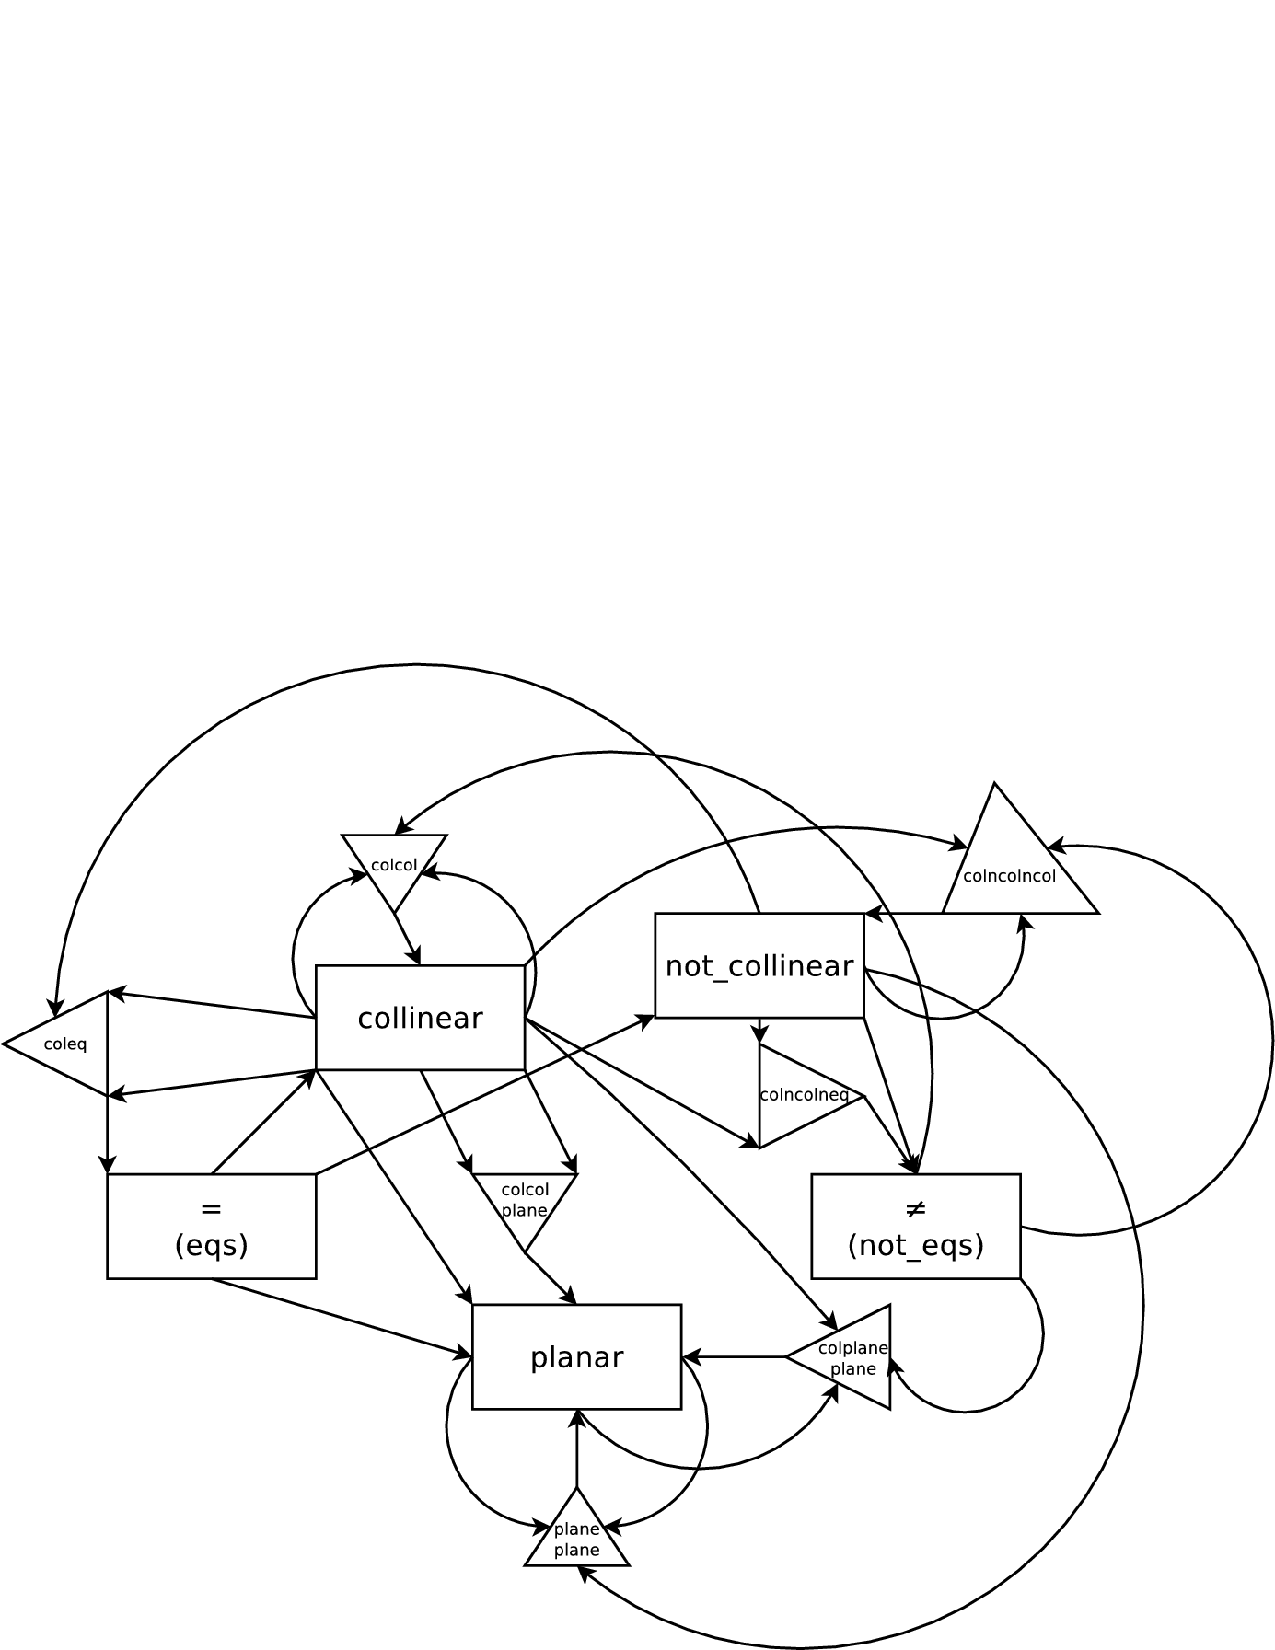
\includegraphics[scale=0.5]{automation/DataFlow}
\caption{Data-flow for incidence reasoning. The five boxes represent our five lists of data, while triangles represent inference rules}
\label{fig:DataFlow}
\end{figure}

Our aim in this section will be to show how such data-flows can be expressed declaratively in a suitable combinator language. Combinator languages are a staple of typed functional programming and LCF theorem provers, which already boast powerful combinators for conversions and tactics~\cite{Tactics}. By following the example of such languages, we hope to contribute a library that has a potentially wider application than the peculiar incidence automation we need for our verifications. The incidence automation will be just one possible hand-crafted \emph{discoverer} written in this language, just as hand-crafted tactics are written in tactic languages.

The advantage of choosing a combinator language, as opposed to some other kind of domain-specific language, is that it fully integrates with the host programming language, and is therefore easy to integrate with the tactic combinator language and the Mizar~Light combinator language. The user is also free to extend the language by defining derived combinators, and can easily inject their own computations into the language using lambda abstraction.

\subsection{Related Work}
The idea of an algebraic data-flow language was considered early on by Chen~\cite{ChenForwardChaining}, who gave a specification for a variety of primitives very similar to our own, though without an implementation. Since then, algebras for logic programming, handling unbounded and fair search have been developed~\cite{BacktrackingMonad,Omega}, but these lack strong guarantees on the order in which elements are found, and can be unpredictable.

An equivalent version of the algebra we shall consider here was originally conceived of by Spivey~\cite{SpiveyBreadthFirst}. It has been used recently by Katayama~\cite{ImprovementsMagickHaskeller} to perform exhaustive searches of functional programs, and its theoretical underpinnings have been rigorously developed~\cite{SearchAlgebras}. Unlike the other logic programming monads, it has much stronger constraints on the order in which values are searched for. 

Our own algebra generalises Spivey's implementation somewhat by replacing his \emph{bags} with more general collections, and we take advantage of this generalisation in \S\ref{sec:Trees}. Moreover, our own realisation of this algebra offers a more ``operational'' motivation of the definitions to complement Spivey's.

\subsection{Streams}\label{sec:Streams}
Our overarching purpose is to output data, perhaps to a terminal, to a database to be used during a proof, or perhaps to another consumer for further processing. If we think of this output \emph{as} the implementation, then we are dealing with procedures which lazily generate successive elements of a list. For the purposes of the theory, we assume that the lazy lists are infinite \emph{streams}. These shall be the primitives of our data-flow algebra.

For now, we leave unspecified what computations are used to generate the primitive streams. It might be that a stream simply echoes a list of precomputed data; it might generate data based on standard input; it might generate them from some other automated tool. We shall focus instead on transformations for streams, and in how we might lift the typical symbolic manipulation used in theorem proving to the level of streams.

One reason why streams and lazy lists are a good choice here is that they generalise \emph{the} ubiquitous data-structure of ML and its dialects, and have rich interfaces to manipulate them. A second reason why they are an obvious choice is that they have long been known to satisfy a simple set of algebraic identities and thus to constitute a monad~\cite{MonadWadler}. We can interpret this monad as decorating computations with non-deterministic choice and backtracking search.

Monads themselves have become a popular and well-understood abstraction in functional programming. Formally, a monad is a type constructor $M$ and three operations 
\begin{align*}
&\code{return} : \alpha \rightarrow M\;\alpha\\
&\code{fmap} : (\alpha \rightarrow \beta) \rightarrow M\;\alpha \rightarrow M\;\beta\\
&\code{join} : M\;(M\;\alpha) \rightarrow M\;\alpha
\end{align*}
satisfying the algebraic laws given in Figure~\ref{fig:MonadLaws}.

\begin{figure}
\begin{align}
&\code{fmap}\;(\lambda x.\;x)\;m = m\notag\\
&\code{fmap}\;f \circ \code{fmap}\;g = \code{fmap}\;(f \circ g)\notag\\
&\code{fmap}\;f \circ \code{return} = \code{return}\circ f\notag\\
&\code{fmap}\;f \circ \code{join} = \code{join} \circ \code{fmap}\;(\code{fmap}\;f)\notag\\
&(\code{join} \circ \code{return})\;m = m\notag\\
&(\code{join} \circ \code{fmap}\;\code{return})\;m = m\notag\\
&\code{join} \circ \code{join} = \code{join} \circ \code{fmap}\;\code{join} \label{eq:JoinAssoc}
\end{align}
\caption{The monad laws}
\label{fig:MonadLaws}
\end{figure}

The monad that is typically defined on lists can be used for search, but it takes concatenation $\code{concat} : [[\alpha]] \rightarrow [\alpha]$ for its \code{join} operation. This makes it unsuitable for \emph{fair} and \emph{unbounded search} with infinite streams. If the stream $xs$ represents one unbounded search, then we have $xs + ys = xs$ for any $ys$, and thus, all items found by $ys$ are lost.\footnote{Here, $+$ is just list and stream append.} This is to be expected, since the definition of this standard monad corresponds to \emph{depth-first search}. 

\subsection{A Monad for Breadth-First Search}\label{sec:StreamMonad}
There is an alternative definition of the monad which is breadth-first and thus handles unbounded search. Here, the \code{join} function takes an infinite stream of infinite streams, and produces an exhaustive enumeration of all elements. We show how to achieve this in Figure~\ref{fig:ShiftGen} using a function $\code{shift}$, which moves each stream one to the ``right'' of its predecessor. We can then exhaustively enumerate every element, by enumerating each column, one-by-one, from left-to-right. 

\begin{figure}
  \small
  \centering
  \begin{tabular}{rl}
    shift &
    \begin{tabular}{ccccccc}
      $[[D_{0,0},$ & $D_{0,1},$ & $D_{0,2},$ & $\ldots,$ & $D_{0,n},$ & $\ldots],$ \\
      $[[D_{1,0},$ & $D_{1,1},$ & $D_{1,2},$ & $\ldots,$ & $D_{1,n},$ & $\ldots],$ \\
      $[[D_{2,0},$ & $D_{2,1},$ & $D_{2,2},$ & $\ldots,$ & $D_{2,n},$ & $\ldots],$ \\
      $[[D_{3,0},$ & $D_{3,1},$ & $D_{3,2},$ & $\ldots,$ & $D_{3,n},$ & $\ldots],$ \\
      $[[D_{4,0},$ & $D_{4,1},$ & $D_{4,2},$ & $\ldots,$ & $D_{4,n},$ & $\ldots],$ \\
      $[[D_{5,0},$ & $D_{5,1},$ & $D_{5,2},$ & $\ldots,$ & $D_{5,n},$ & $\ldots],$ \\
      & & & & & \vdots
    \end{tabular}\\\\
    = &
    \begin{tabular}{ccccccccccccc}
      $[[D_{0,0},$ & $D_{0,1},$ & $D_{0,2},$ & $D_{0,3},$ & $D_{0,4},$ & $D_{0,5},$ & $D_{0,6},$ & \colorbox{gray}{$D_{0,7},$} & $D_{0,8},$ & $\ldots],$\\
      & $[D_{1,0},$ & $D_{1,1},$ & $D_{1,2},$ & $D_{1,3},$ & $D_{1,4},$ & $D_{1,5},$ & \colorbox{gray}{$D_{1,6},$} & $D_{1,7},$ &  $\ldots],$\\
      && $[D_{2,0},$ & $D_{2,1},$ & $D_{2,2},$ & $D_{2,3},$ & $D_{2,4},$ & \colorbox{gray}{$D_{2,5},$} & $D_{2,6},$ & $\ldots],$\\
      &&& $[D_{3,0},$ & $D_{3,1},$ & $D_{3,2},$ & $D_{3,3},$ & \colorbox{gray}{$D_{3,4},$} & $D_{3,5},$ & $\ldots],$\\
      &&&& $[D_{4,0},$ & $D_{4,1},$ & $D_{4,2},$ & \colorbox{gray}{$D_{4,3},$} & $D_{4,4},$ & $\ldots],$\\
      &&&&& $[D_{5,0},$ & $D_{5,1},$ & \colorbox{gray}{$D_{5,2},$} & $D_{5,3},$ & $\ldots],$\\
      &&&&&& $[D_{6,0},$ & \colorbox{gray}{$D_{6,1},$} & $D_{6,2},$ & $\ldots]$\\
      &&&&&&&         &        & $\vdots$ &           &        &           
    \end{tabular}
  \end{tabular}
  \caption{Shifting}
  \label{fig:ShiftGen}
\end{figure}

If we understand these streams as the outputs of a discoverer, then the outer stream can be understood as the output of a discoverer which \emph{discovers discoverers}. The \code{join} function can then be interpreted as \emph{forking} each discoverer at the point of its creation and combining the data into the output of a single discoverer. The highlighted column in Figure~\ref{fig:ShiftGen} is this combined result: a set of values generated simultaneously and thus having no specified order (this is required to satisfy Law~\ref{eq:JoinAssoc} in Figure~\ref{fig:MonadLaws}).

However, this complicates our stream type, since we now need additional inner structure to store the combined values. We will refer to each instance of this inner structure as a \emph{generation}, following our terminology from \S\ref{sec:ForwardChaining}. Each generation here is a finite collection of simultaneous values discovered at the same level in a breadth-first search. We just need to define the \code{join} function, taking care of this additional structure.

Suppose that generations have type $G\;\alpha$ where $\alpha$ is the element type. The manner in which we will define our \code{shift} and \code{join} functions on streams of generations assumes certain algebraic laws on the generations: firstly, they must constitute a monad; secondly, they must support a sum operation \mbox{$(+):G\;\alpha\rightarrow G\;\alpha\rightarrow G\;\alpha$} with identity~$0:G\;\alpha$. 

The \code{join} function for streams must then have type $[G\;[G\;\alpha]] \rightarrow [G\;\alpha]$, sending a stream of generations of streams into a stream of generations of their data. To define it, we denote the $k^{\text{th}}$ element of the argument to \code{join} by $gs_k = \{d_{k,0}, d_{k,1}, \ldots, d_{k,n}\}$ of type $G\;[G\;\alpha]$. Each $d_{k,i}$ is, in turn, a stream $[g^k_{i,0}, g^k_{i,1}, g^k_{i,2}, \ldots] : [G\;\alpha]$. We invert the structure of $gs_k$ using a function $\code{transpose}  : M[\alpha]\rightarrow [M\;\alpha]$. This function generalises matrix transposition on square arrays (type $[[\alpha]]\rightarrow[[\alpha]]$) to arbitrary monads $M$, and the generality allows us to abstract away from Spivey's bags and consider more exotic inner data-structures.\footnote{The operator \code{::} is \emph{cons} for lists and streams.}
\begin{displaymath}
\code{transpose}\;xs = \cons{\code{fmap}\;\code{head}\;xs}{\code{transpose}\; (\code{fmap}\;\code{tail}\;xs)}.
\end{displaymath}

The transpose produces a stream of generations of generations (type $[G\;(G\;\alpha)]$). If we join each of the elements, we will have a stream $[D_{k,0}, D_{k,1}, D_{k,2}, \ldots] : [G\;\alpha]$ (see Figure~\ref{fig:Transpose}), and thus, the shift function of Figure~\ref{fig:ShiftGen} will make sense. Each row is shifted relative to its predecessor by prepending the 0 generation, and the columns are combined by taking their sum.

\begin{figure}
  \begin{align*}
    &\code{map}\;\code{join}\;(\code{transpose}\;\{d_{k,0}, d_{k,1}, \ldots, d_{k,n}\})\\
  = &\code{map}\;\code{join}\;\left(\code{transpose}\;\left\{\begin{matrix}
        [g^k_{0,0}, & \colorbox{gray}{$g^k_{0,1}$}, & g^k_{0,2}, &\ldots]\\
        [g^k_{1,0}, & \colorbox{gray}{$g^k_{1,1}$}, & g^k_{1,2}, &\ldots]\\
                  & \vdots\\
        [g^k_{n,0}, & \colorbox{gray}{$g^k_{n,1}$}, & g^k_{n,2}, &\ldots]
      \end{matrix}\right\}\right)\\
      = &\left[\begin{matrix}
        \code{join}&\{g^k_{0,0}, & g^k_{1,0}, &\ldots, & g^k_{n,1}\},\\
        \code{join}&\Big\{\colorbox{gray}{$g^k_{0,1}$}, & \colorbox{gray}{$g^k_{1,1}$}, &\colorbox{gray}{$\ldots$}, & \colorbox{gray}{$g^k_{n,1}$}\Big\},\\
        \code{join}&\{g^k_{0,2}, & g^k_{1,2}, &\ldots, & g^k_{n,2}\},\\
                   & \vdots
                 \end{matrix}\right]\\
      \quad= &[D_{k,0}, D_{k,1}, D_{k,2}, \ldots]
  \end{align*}
\caption{\code{transpose} and \code{join}}
\label{fig:Transpose}
\end{figure}

The type of streams now constitutes a monad (see Spivey~\cite{SearchAlgebras} for details). The fact that we have a monad affords us a tight integration with the host language in the following sense: we can lift arbitrary functions in the host language to functions on streams, and combine one stream $xs : [G\;\alpha]$ with another stream $xs' : \alpha \rightarrow [G\;\beta]$ which depends, via arbitrary computations, on each individual element of $xs$. 

There is further algebraic structure in the form of a monoid:\footnote{A structure with an associative operation and identity.} streams can be summed by summing corresponding generations, an operation whose identity is the infinite stream of empty generations. 

\section{Case-analysis}\label{sec:CaseAnalysis}
Our algebra allows us to partition our domain into discoverer streams according to our own insight into a problem, and compose them in a way that reflects the typical reasoning patterns found in the domain. For incidence reasoning, we divide the domain into our five kinds of data discoverer, and combine the discoverers using our rules.

We wanted more than this, however, because when it comes to theorem-proving, the data is further partitioned as we perform case-analyses on disjunctions. In proof-search, when we encounter a disjunction, we will want to branch the search and associate data in each branch with its own disjunctive hypothesis. 

Ideally, we want to leave such case-splitting as a book-keeping issue in our algebra, and so integrate it into the composition algorithm. Streams must then record a context for all of their data, and this context must be respected as the streams are combined. 

Our definitions give us the flexibility to implement this. We can choose a data-structure other than bags for the generations, and to solve the problem of case-analysis, we have chosen to implement the generations as \emph{trees}. 

\subsection{Trees}\label{sec:Trees}
Each tree represents a generation of data partitioned according to case-splits. Each node in a tree is a bag of data discovered in that generation under a disjunctive hypothesis. Branches correspond to case-splits, with each branch labelled for the disjunct on which case-splitting was performed. The branch labels along any root-path therefore provide a context of disjunctive hypotheses for that subtree. For example, the tree in Figure~\ref{fig:BasicTreeExample} might represent formula~\ref{eq:CaseAnalysisTreeFormula}, made by case-analysing \mbox{$P \vee (Q \wedge (R \vee S))$}. Our goal is to discover data which hold when the case-splits are eliminated.

\begin{equation}\label{eq:CaseAnalysisTreeFormula}
\begin{aligned}
\phi_1 \wedge \phi_2 \wedge \cdots \wedge \phi_n &\wedge (P \implies \psi_1 \wedge \psi_2 \wedge \cdots \wedge \psi_n)\\
&\wedge \left(\begin{aligned} Q \implies \chi_1 \wedge \chi_2 \wedge \cdots \chi_n &\wedge (R \implies \alpha_1 \wedge \alpha_2 \wedge \cdots \wedge \alpha_n)\\ &\wedge (S \implies \beta_1 \wedge \beta_2 \wedge \cdots \wedge \beta_n)\end{aligned}\right).
\end{aligned}
\end{equation}

\subsubsection{Combining Trees}\label{fig:CombiningTrees}
\begin{figure}
\centering\includegraphics[scale=0.7]{automation/BasicTreeExample}
\caption{A simple tree branching on case-splits}
\label{fig:BasicTreeExample}
\end{figure}

The principal operation on trees is a sum function which is analogous to the append function for lists and streams, combining all data from two trees. The simplest way to combine two trees, one which yields a monad, has us nest one tree in the other. That is, we replace the leaf nodes of one tree with copies of the other tree, and then flatten. For definiteness, and to ensure associativity, we always nest the right tree in the left. See Figure~\ref{fig:TreeNesting}.

\begin{figure}
\centering\includegraphics[scale=0.7]{automation/FullSimpTree1}
\caption{Combining trees by nesting}
\label{fig:TreeNesting}
\end{figure}

Even if we only had a constant number of case-splits, successive combining in this manner would yield trees of arbitrarily large topology, which is clearly not desirable. As such, we need some way to simplify the resulting trees. Our hard constraint is that we must not lose any information: if data is deleted from the tree, it must be because it is trivially implied by other data in the tree. Our softer constraint, which we do not attempt to formally define, is that the topologies should represent a reasonably efficient partitioning of the proof-space according to the combination of case-analyses.

Our first means of simplification is a form of weakening. If we have tree $t$ which branches on a disjunctive hypothesis and which contains a subtree $t'$ branching on that same hypothesis, then the root path is of the form 
\begin{displaymath}
P \implies \cdots \implies Q \implies \cdots \implies Q \implies \phi.
\end{displaymath}
We eliminate the redundant antecedent by folding $t'$ into its immediate parent. Any siblings of $t'$ whose branch labels are not duplicated along the root path are then discarded. They will be left in the other branches of $t$.

The situation is shown in Figure~\ref{fig:TreeWeakening}, where we have coloured duplicate hypotheses along root paths. In the result, we fold the marked subtrees into their parents, and discard the siblings. Notice that no data has been lost, and no individual bags at tree-nodes have been changed: the only operations we use here are topological changes to the tree, and bag union $(+)$.

\begin{figure}
\centering\includegraphics[scale=0.6]{automation/FullSimpTree2}
\caption{Weakening}
\label{fig:TreeWeakening}
\end{figure}

Our next simplification allows us to delete a subtree $t$ if its branch case is already considered by an uncle\footnote{The sibling of a parent node.} $t'$. All theorems of $t$ will appear in $t'$ where the topology will have been simplified in our weakening step. The situation is shown in Figure~\ref{fig:TreeRedundantSplits}. The $P$ branch on the left-hand side is uncle to the $P$ branches on the right. These latter branches are therefore pruned.

\begin{figure}
\centering\includegraphics[scale=0.7]{automation/FullSimpTree3}
\caption{Removing redundant case-splits}
\label{fig:TreeRedundantSplits}
\end{figure}

Finally, we can promote data that appears at all branches. In Figure~\ref{fig:TreeRedundantSplits}, the $xs'$ bag of theorems appears in every node at the same level, and so can be promoted into the parent, corresponding to disjunction elimination. 

Our final tree is shown in Figure~\ref{fig:TreePromoting}. We have described our simplification in several steps, though they can be combined into a single pass of the left hand tree. That said, with a single pass, we have not found a way promote \emph{all} data. If we had, the replicated $us'$ bag in the bottom right branches of the tree could be promoted into the $Q$ branch. We will not elaborate on this implementation issue.

\begin{figure}
\centering\includegraphics[scale=0.7]{automation/FullSimpTree4}
\caption{Promoting common data}
\label{fig:TreePromoting}
\end{figure}

\subsubsection{Joining Trees}
Our function which combines trees is a sum function, which has an identity in the empty tree containing a single empty root node. This is enough structure to define a \code{join} function analogous to list and stream concatenation. Suppose we are given a tree $t$ whose nodes are themselves trees (so the type is $\code{Tree}\;(\code{Tree}\; \alpha)$). Denote the inner trees by $t_0$, $t_1$, $t_2$, $\ldots$, $t_n : \code{Tree}\;\alpha$. We now replace every node of $t$ with an empty bag, giving a new tree $t' : \code{Tree}\;\alpha$. We can now form the sum 
\begin{displaymath}
t' + t_0 + t_1 + t_2 + \cdots + t_n.
\end{displaymath}

The resulting tree will then contain discovered data which respect disjunctive hypotheses from their place in $t$ and from their respective inner-trees.

\section{Additional Primitives and Derived Discoverers}\label{sec:Additional}
Using trees as generations, we have a stream data-type to represent a discoverer searching a space which has been partitioned according to case-splits. Since we do not specify what sort of data we are considering, our discoverers have polymorphic type. We alias the type as $\code{discoverer}\ \alpha$. 

As we described in \S\ref{sec:StreamMonad}, these discoverers form a monoid. Operationally, the sum function runs two discoverers in parallel, respecting their mutual case-splits, while our identity discovers nothing but empty generations.

We now explain additional functionality, some of which relates specifically to theorem proving and some of which more generally handles filtering. The following material, so far as we are aware, is new.

\subsection{Case-splitting}
Case-splits are introduced by our function $\code{disjuncts}$, which is a discoverer parameterised on arbitrary sequents. Here, $\code{disjuncts}\left(\Gamma \vdash P_1 \vee P_2 \vee \cdots \vee P_n\right)$ is a stream containing a single tree with $n$ branches from the root node. The $i^{th}$ branch is labelled with the term $P_i$ and contains the single sequent $\Gamma \cup \{P_i\} \vdash P_i$. This process can be undone by flattening trees using $\code{flatten}$, which discharges all tree labels and adds them as antecedents in the right hand side of all sequents.

\subsection{Delaying}
A generation can be ``put off'' to a later generation using the function $\code{delay}$. In terms of streams, this function has the trivial definition
\begin{displaymath}
  \code{delay}\ xs = \cons{\emptyset}{xs}.
\end{displaymath}
The use of this function is actually essential when writing mutually recursive discoverers. If one discoverer outputs data based on data output by another discoverer, and \emph{vice versa}, then one of the two discoverers must be delayed to avoid deadlock.

\subsection{Filtering}\label{sec:Filtering}
In many cases, we will not be interested in all the outputs generated by a discoverer. Fortunately, filtering is a library function for monads with a zero element, and can be defined in terms of the usual bind operation ($\bind$). We give definitions for both $(\bind)$ and $\code{filter}$ as follows:
\begin{align*}
xs \bind f &= \code{join}\;(\code{fmap}\;f\;xs) \\
\code{filter}\;p\;xs &= xs \bind (\lambda x.\;\code{if } p\;x \code{ then } \code{return}\;x \code { else } 0).
\end{align*}

More challenging is a function to perform something akin to \emph{subsumption}. The idea here is that when a sequent is discovered which ``trivially'' entails a later sequent, the stronger sequent should take the place of the weaker. This is intended only to improve the performance of the system by discarding redundant search paths based on subsumed sequents. 

We can generalise the idea to arbitrary data-types, and parameterise the filtering by any partial-ordering on the data, subject to suitable constraints. One intuitive constraint is that a stronger item of data should only replace a weaker item so long as we do not ``lose'' anything from later discovery. Formally, we require that any function $f$ used as the first argument to \code{fmap} is monotonic with respect to the partial-order. That is, if $x \leq y$ then $f(x) \leq f(y)$. 

We then implement ``subsumption'' as the transformation \code{maxima}. This transforms a discoverer into one which does two things: firstly, it transforms every individual generation into one containing only maxima of the partial-order. Secondly, it discards data in generations that is strictly weaker than some item of data from an earlier generation. To handle case-splits, we assert that data higher up a case-splitting tree is always considered stronger than data below it (since it carries fewer case-splitting assumptions).

\subsubsection{More Sophisticated Filtering}
There are two pieces of missing optimisation. Suppose we have data $x$ and $y$ where $x \leq y$ and a stream $xs = \left[\{x\}, \{y\}\right].$ That is, $xs$ represents a discoverer which produces two generations of data. In the first generation is the single datum $x$ and in the second is the single datum $y$. Now suppose we have a function $f$ which happens to have the mappings
\begin{align*}
x &\mapsto \left[\{\},\{\},\{\},\{\},\{x'\}\right]\\
y &\mapsto \left[\{y'\}\right].
\end{align*}

Here, $y$ is sent immediately to the new datum $y'$, while the image $x'$ of $x$ takes some time to generate, represented here by a succession of four empty generations. Thus,
\begin{displaymath}
xs \bind f = \left[\{y'\}, \{\}, \{\}, \{\}, \{x'\}\right].
\end{displaymath}

What happens when we want to take the maxima of this stream? To do this, $f$ must be monotonic, and to verify this, we need some way to partially order the images of $f$, which means knowing more generally how to partially order discoverers.

In general, if two discoverers $xs$ and $ys$ are such that $xs \leq ys$, what should we say this implies about the ordering of the items discovered by each? We should be able to say at least this much: for every $w$ in the first $n$ generations of $xs$, there should exist some $z$ in the first $n$ generations of $ys$ such that $w \leq z$. Thus, $ys$ discovers data which is at least as strong as the data of $xs$, and does so at least as early in terms of the number of generations.

So if by monotonicity we require that $\left[\{\},\{\},\{\},\{\},\{x'\}\right] \leq \left[\{y'\},\{\}\right]$, then we further require that $x' \leq y'$. Therefore:
\begin{displaymath}
\code{maxima}\ xs \bind f = \code{maxima}\ \left(\left[\{y'\}, \{\}, \{\}, \{\}, \{x'\}\right]\right) = \left[\{y'\}, \{\}, \{\}, \{\}, \{\}\right].
\end{displaymath}
And here we have a problem: the delayed and potentially slow computation of $x'$ was wasted. Once $y$ was discovered, further discovery based on $x$ should have been halted. This does not happen in our implementation, and leads to a great deal of wasted effort. Consider the fact that every time we successfully apply Rule~\code{colcol} to take the union of sets $S$ and $T$, all further discovery based on $S$ and $T$ should be abandoned in favour of discovery using $S \cup T$. A similar issue applies to the discovery of equalities: as new equalities are discovered, they should rewrite all other data and ongoing discovery based on unwritten data should be abandoned.

A second piece of potentially desirable functionality is a form of \emph{memoisation}. Suppose two generations of a discoverer are evaluated to $[\{x\}, \{y\}]$ where $x \leq y$. With $y$ evaluated, we would probably prefer any reevaluation of this discoverer to actually replace $x$, yielding $[\{y\}, \{\}]$. 

This additional functionality has not yet been implemented, and to get it to work, we might have to significantly modify the underlying data-structures for our streams. We leave such possibilities to future work.

\subsection{Accumulating}\label{sec:Accumulating}
We supply an accumulation function which is similar to the usual \code{fold} function on lists and streams. This threads a two-argument function through the data in a stream, starting with a base-value, and folding each generation down to a single intermediate datum. Thus, we have:
\begin{align*}
\code{accum}\;(+)\;0\;[\{1,2\}, \{3,4\}, \{5\}, \{6,7,8\}] 
&= [\{0 + 3\}, \{3 + 7\}, \{10 + 5\}, \{15 + 21\}]\\
&= [\{3\}, \{10\}, \{15\}, \{36\}].
\end{align*}

One useful case of this allows us to gather up all data discovered so far in a single collection. If the collection is finite lists, we just use $\code{accum}\;(\lambda xs.\;\lambda x.\;x :: xs)\;[\,]$.

% \subsection{Normalisation}
% For efficiency, it will be useful to normalise with respect to any discovered equalities and simple rewrite rules. 

\subsection{Deduction}
Direct deduction, or \emph{modus ponens}, is the basis of forward-chaining and we provide two main ways to lift it into the type of discoverers. 

We first have to deal with \emph{exceptions}. In HOL~Light, the \emph{modus ponens} inference rule will throw an exception if its arguments are of incorrect form, so we first redefine \code{fmap} to filter thrown exceptions out of the discovery. It is generally undesirable to let exceptions propagate upwards, since this would lead to an entire discoverer being halted. 

With \code{fmap} redefined as \code{fmap'}, we can define functions $\code{fmap2}'$ and $\code{fmap3}'$ which lift two and three-argument functions up to the level of discoverers, also filtering for exceptions.
\begin{align*}
\code{fmap}'\;f\;xs &= xs \bind (\lambda x.\;\code{try}\; \code{return}\;(f\;x)  \code{ with \_ } \rightarrow 0)\;xs\\
\code{fmap2}'\;f\;xs\;ys &= \code{fmap}\;f\;xs \bind (\lambda f.\;\code{fmap}'\;f\;ys)\\
\code{fmap3}'\;f\;xs\;ys\;zs &= \code{fmap}\;f\;xs \bind (\lambda f.\;\code{fmap2}'\;f\;ys\;zs).
\end{align*}
With these, we can define the following forward-deduction functions:
\begin{align*}
\code{chain1}\;imp\;xs &= \code{fmap2}'\; \code{MATCH\_MP}\; (\code{return}\;imp)\;xs \\
\code{chain2}\;imp\;xs\;ys &= \code{fmap2}'\; \code{MATCH\_MP}\; (\code{chain1}\; imp\;xs)\;ys\\
\code{chain3}\;imp\;xs\;ys\;zs &= \code{fmap2}'\; \code{MATCH\_MP}\; (\code{chain2}\;imp\;xs\;ys)\;zs\\
\code{chain}\;imps\;xs &= imps \bind (\lambda imp.\;\code{if is\_imp } imp\\ &\code{then } \code{chain}\;(\code{fmap}\;(\code{MATCH\_MP}\;imp)\;thms)\;thms\\
&\code{else } \code{return}\; imp).
\end{align*}

The function \code{is\_imp} is a standard HOL~Light function which returns \code{true} if the right hand side of its sequent argument is an implication, while $\code{MATCH\_MP}$ is the matching \emph{modus ponens} derived inference rule
\begin{displaymath}\infer[\code{MATCH\_MP}]{\Gamma\cup\Delta \vdash Q'}{\Gamma \vdash P \implies Q&\Delta \vdash P'}
\end{displaymath}
where $P'=P[\theta]$ and $Q'=Q[\theta]$ for some substitutiton $\theta$. 

Thus, \code{chain1} takes a sequent $\Gamma \vdash P \implies Q$ and applies \emph{modus ponens} across a discoverer of antecedent sequents. The function \code{chain2} takes a sequent of the form $\Gamma \vdash P \implies Q \implies R$ and applies \emph{modus ponens} across two discoverers of antecedents. The function \code{chain3} takes a sequent of the form $\Gamma \vdash P \implies Q \implies R \implies S$ and applies \emph{modus ponens} across three discoverers of antecedents. The final, more general \code{chain} function, recursively applies implication sequents with arbitrary numbers of curried antecedents from the discoverer $imps$ across all possible combinations of antecedents from the discoverer $xs$.%, reproducing the behaviour of \sec{sec:Example}.

Note that the discoverers \code{chain1}, \code{chain2} and \code{chain3} will not necessarily try all combinations of theorems from their arguments. They fail opportunistically, attempting \emph{modus ponens} on each sequent from the first argument, and \emph{only if it succeeds}, attempting \emph{modus ponens} on sequents from the second argument. This is a happy feature of the data-driven semantics of monads (but see \S\ref{sec:Applicative} for its drawbacks). 

It is therefore sensible to order the antecedents of the implication according to how likely they are to succeed. Antecedents which rarely succeed should appear early to guarantee a quick failure. In our use case, for example, we apply Rule \code{coleq} from \S\ref{rule:coleq} with the collinear antecedents before the non-collinear antecedent, since there are generally many more non-collinear sequents to choose from than there are collinear sequents.

% CHAIN_MP, CHAIN1, CHAIN2, CHAIN3

% Not listed are functions based on Modus Ponens (\code{mp}). These functions we have called \code{chain1}, \code{chain2}, \code{chain3}, and so on, each written in one line of code in terms of its predecessor. The function \code{chain\_n} takes an implicational rule with $n$ antecedents, and yields a function which takes $n$ antecedent discoverers to produce a conclusion discoverer. 

% Our implementation allows for some interesting control of the search when discoveres are combined in this way. Antecedents in the original rule are matched one at a time, and conjunctions are split after each match. By carefully ordering and interleaving antecedents in the original rule around conjunctions, the user can control the search strategy. For example, suppose we create functions of three chains by applying 

% \noindent\code{   chain3 : thm $\rightarrow$ thm chain $\rightarrow$ thm chain $\rightarrow$ thm chain $\rightarrow$ thm chain} 

% \noindent to the equivalent rules:
% \begin{align*}
% &(P \rightarrow S \rightarrow Q \rightarrow X) \wedge (Q \rightarrow T \rightarrow P \rightarrow Y)
% \shortintertext{and}
% &P \rightarrow Q \rightarrow (S \rightarrow X \wedge T \rightarrow Y)
% \end{align*}

% The two resulting functions will differ in how they perform search on their three argument chains, in a potentially significant way. The first will simultaneously try to match $P$ and $Q$ in the first discoverer. Successful matches will respectively match $S$ and $T$, and then finally $Q$ and $P$. However, the second function will only try to match $P$. If successful, it will then match $Q$, and if that is successful, it will try to match $S$ and $T$ simultaneously. 

% The first formulation may be preferred when $P$ and $Q$ are equally likely to match and matches against $S$ and $T$ depend respectively on whether $P$ and $Q$ match. The second formulation would be preferred if $P$ is much less likely to match than $Q$ and there is no such dependence.

% This completes our overview of the discovery language. A user can now build discovery engines directly from these functions and primitives. This is very much in the spirit of HOL~Light and its LCF~\cite{LCF} foundation, where inference rules, tactic languages and rewrite engines are ordinary functions and combinator languages~\cite{Tactics}. Shallow-embedded tools can be a challenge for new users, but they offer enormous expressive power in a rich programming language, and allow different parts of the system to seamlessly integrate. 

\section{Integration}
It is straightforward to integrate our discoverers with the rest of HOL~Light's proof tools. We can, for example, lift term-rewriting to the level of discoverers simply by lifting HOL~Light's rewriting functions with \code{fmap} and its derivatives. 

To use our discoverers in declarative proofs, we introduce two Mizar~Light primitives. The first, \code{obviously}, is used to assist any step in a declarative proof via a discoverer.\footnote{The type \code{thm} is the type of HOL~Light sequents. The type \code{step} is the type of Mizar~Light steps.}
\begin{displaymath}
  \code{obviously}\;:\;(\code{discoverer}\ \code{thm}\rightarrow\code{discoverer}\ \code{thm}) \rightarrow step \rightarrow step.
\end{displaymath}

The expression $\code{obviously}\  f$ transforms a step into one which lifts the step's justifying theorems into a discoverer, applies the transformation $f$ to this discoverer, and then retrieves all discovered theorems to a certain depth. These are then used to supplement the step's justification.

By allowing $f$ to have type $\code{discoverer}\ \code{thm}\rightarrow\code{discoverer}\ \code{thm}$, we can use a discovery pipeline via function composition to justify a declarative step. For example, later in our formal development we will introduce an incidence discoverer $\code{by\_incidence}$. We also have a function $\code{split}$  which recursively breaks conjunctions and splits disjunctions across all sequents found by a given discover. Finally, we have a rule $\code{add\_triangles}$ which introduces non-collinearity sequents from sequents about points inside and outside triangles. The three functions can be pipelined in a single step by writing
\begin{displaymath}
\code{obviously}\ (\code{by\_incidence}\circ \code{add\_triangles}\circ \code{split}) \ldots.
\end{displaymath}

Next, we introduce a primitive $\code{clearly}$. This has the same type as $\code{obviously}$, but rather than collecting all discovered sequents, it searches specifically for the formula to be obtained by a Mizar~Light step (in the case of a $\code{qed}$ step, this is the goal formula). When the \code{clearly} primitive is used, it leaves the basic Mizar~Light justification tactic with a trivial proof.

\label{sec:DiscoverTac}
Finally, we have introduced a theorem-tactic \code{discover\_tac} with type
\begin{multline*}
\code{discover\_tac}\;:\;(\code{discoverer}\ \code{thm}\rightarrow\code{discoverer} \ \code{thm}) \\\rightarrow ([\code{thm}] \rightarrow \code{tactic}) \rightarrow \code{tactic}.
\end{multline*}
As with $\code{obviously}$ and $\code{clearly}$, we take a transformation of discoverers. Then when we apply $\code{discover\_tac}\ f\ tac$,  all goal hypotheses are fed to $f$. The resulting discovered sequents are then supplied to the function $tac$ (often just $\code{MESON}$).

\subsection{Concurrency}\label{sec:Concurrency}
In \S\ref{sec:NaiveConcurrency}, we hinted at the possibility of making our algorithm concurrent and collaborative. The implementation is straightforward with streams.

So that discoverers can incorporate the user's manual proof efforts, they need a way to inspect the proof context. We use a simple new primitive discoverer $\code{monitor}$ to allow this. As we stated in our introduction in \S\ref{sec:Streams}, primitive discoverers can generate their outputs in whatever manner they want. Our $\code{monitor}$ just regularly examines the proof context and outputs its hypotheses. We ensure that only unique hypotheses are ever generated by using the function $\code{maxima}$.

For the user's inspection, discovered theorems are output to the terminal one-by-one, simply by iterating over the streams with an ordinary print function in a separate thread. Additionally, this thread updates a reference cell \code{the\_facts} which holds all theorems discovered in that thread so far. The cell can be deferenced in the interactive proof, so that the user can make use of the results of concurrent discoverers as they come in.

To complete the architecture, we provide signalling commands that can tell a discovery thread to pause, thereby freeing up CPU resources, to resume from a pause, or to change to an alternative theorem discoverer, so that the thread does not have to be killed.

We should admit to a caveat here. Generations, as we have implemented them, are not generally usable across the branches of case-splits and subproofs of a declarative verification. When the user completes a branch or subproof, some of their assumptions will no longer be in force. Thus, the user can no longer apply data generated from those assumptions to justify the next proof step. If they try to do so, Mizar~Light will throw an error when the step command is processed, as part of the basic validity checking of the tactic system. Instead, the user must manually reset the discoverers after each case-split and subproof, to throw out the assumptions no longer in force. This is far from ideal, but as yet, our implementation does not address the issue.

% \begin{figure}
% {\scriptsize\input{incidence}}
% \caption{Incidence Discovery in ML}
% \label{fig:MLEngine}
% \end{figure}

\subsection{Dependency Tracking}\label{sec:WriterMonad}
While writing a proof, we would normally start our incidence discoverer concurrently, which would generate sequents as we worked. The discoverer would consider all of our goal hypotheses, and would typically find a large number of sequents, most of which were not needed in the proof. Of those which were needed, we wanted to know the specific subset of hypotheses from which they were derived. This is desirable when it comes to proof-replay, when we would like the discoverer to work more efficiently with just the hypotheses it needs. But it is also desirable in terms of writing declarative proofs: we want to write the dependent hypotheses directly into the proof script, so they are apparent to the reader. To achieve this, we need our discoverers to track hypotheses.

A nice feature of monads in functional programming is that, when defined in the form of a \emph{transformer}, the extra book-keeping can be added in a clean and modular way. In this case, we create a generic \emph{writer transformer}.

\emph{Writer} is a monad with extra functions for \emph{writing} values from any monoid during a computation, and for running computations to retrieve the final written values. It provides a modular way to introduce things such as \emph{logging} into computations. So if we have a computation which writes the value \code{"Hello"} and returns the value 1, and another computation which writes the value \code{" world!"} and returns the value 2, then when we lift addition over the two computations, we have a computation which returns the value 3 and writes \code{"Hello world!"}. The monoid here is strings with the append operation.

Writer can be defined as a transformer which, when applied, is made to write values inside any other monad. We made our writer work on a monoid of hypothesis sets with the union operation. These sets contain the dependent hypotheses from the proof context for every discovered sequent, and they automatically accumulate as discoverers are combined. We do not need to write any special logic for this. All the details are handled generically by the writer transformer.

All we need to do is extend the $\code{monitor}$ discoverer to initialise the dependent hypotheses sets. So now, every time $\code{monitor}$ pulls a hypothesis from the proof context, it must also write the hypothesis as a dependency on further computation. The dependencies then automatically propagate.

\section{Implementation Details}
The following section describes some technical challenges we faced. We include it for the sake of honesty, since the presentation of the ideas so far ignores all the bumps that thwart a nice clean implementation in Ocaml. We assume some knowledge of the Ocaml language here.

We have implemented a general monad library in Ocaml, providing a signature for the minimal implementation of an arbitrary monad, and a \emph{functor}\footnote{All uses of the term \emph{functor} here refer to a feature of the Ocaml module system. Though a term borrowed from category theory, it is not in the same context as \emph{monad} as we have used it in this chapter.} to turn this minimal implementation into a richer monad interface with derived functions. Monad transformers are functors between minimal implementations of monads. The stream monad itself is a transformer from an arbitrary monad of generations. If we want to use the bag implementation, we can just supply a module of bags to this transformer. If we want to use our case-splitting implementation, we supply our module of trees. 

These transformations can be stacked. In fact, in our final implementation, we first apply our writer transformer to a monoid of hypotheses sets. The writer transformer is then applied to our tree monad. Finally, the tree monad is applied to our stream monad to produce a stream which discovers theorems, handles case-splits and tracks dependent hypotheses.

\subsection{Implementation Issues}
As of writing, HOL~Light relies heavily on modifications to Ocaml's preprocessor, one of which forces Ocaml's lexer to treat any lexeme which contains more than one upper-case letter as being a lower-case identifier. This plays havoc with the CamelCase naming convention now being adopted in Ocaml's ``Batteries Included'' library, since Ocaml's parser expects all module names to be uppercase. To circumvent this, we supply our own preprocessor which allows for lower-case identifiers in module names. This is only intended as a hack over a hack until we find a robust solution.

Concurrency often raises thorny issues in working code, and some HOL~Light functions were not developed with concurrency in mind. The basic \code{MESON} tactic, which we rely on throughout our verifications, is not thread-safe, and it must be avoided when defining discoverers.

% We have stressed ``concurrency'' in this chapter, rather than ``parallelisation'', since Ocaml only supports the former. This means we get no speed improvements by using threads. This should not be seen as a significant drawback, since such multithreading is inherently dangerous in a language such as Ocaml which allows for uncontrolled side-effects. HOL~Light itself was not developed with multiprocessing support in mind. Its basic \code{MESON} tactic, for instance, is not thread-safe. Even without parallelisation, the tactic must be avoided when implementing discoverers.

Another issue with threading concerns UNIX signals. The standard way to interact with HOL~Light is to run intractable decision procedures on problems. If these procedures fail, the user interrupts them at the Ocaml top-level by sending \code{SIGINT}. If the user is running a concurrent discoverer when they send this signal, it might interrupt the wrong thread, possibly leaving the discoverer with dangling resources. As a quick hack around this behaviour, we trap SIGINT in the discovery thread, pause, and emit it again.

Finally, Ocaml's lazy list library has some unexpected implementation choices. For instance, the list concatenation function $concat\;:\;[[\alpha]]\rightarrow[\alpha]$ is \emph{strict} in its outer list, while the $\code{take}$ function which takes a certain sized prefix of a given lazy list will always force the values in the prefix. These behaviours are generally inappropriate for lazy data-structures, and their use often leads to infinite looping when we come to write recursive functions which generate lazy lists. We have had to rewrite many of them.

Besides these issues, the syntax for lazy lists in Ocaml is cumbersome. Primitive list functions have to explicitly force lazy lists, while recursive lazy lists must be wrapped with a \code{lazy} keyword. One benefit, however, of Ocaml's lazy list implementation is that it detects when a recursive definition requires forcing a vicious circularity. Such a scenario arises when the computation of the first element of $xs$ requires computing the first element of $ys$, and \emph{vice versa}. Such situtations occur easily when writing discoverers in our algebra, and are fixed with choice uses of the $\code{delay}$ function.

\section{Applicative Functors}\label{sec:Applicative}
An idiom or applicative functor $F$~\cite{Applicative} is a generalisation of the monad, which could be thought of as providing at least the ability to lift values with a function $pure\;:\;\alpha \rightarrow F\ \alpha$ and to lift a two argument function as we do with 
\begin{displaymath}
\code{fmap2}\;:\;(\alpha\rightarrow\beta\rightarrow\gamma)\rightarrow F\ \alpha \rightarrow F\ \beta \rightarrow F\ \gamma.
\end{displaymath}

This is actually quite limiting compared to the monad (see \cite{IdiomsArrowsMonads} for a detailed analysis). We can no longer write data-driven computations, such as our $\code{chain}$ functions which automatically fail at the first non-matching antecedent.

That said, because it does not allow data-driven computation, an implementation of the applicative functor interface can potentially be more efficient than the implementation it derives as a generalisation of a monad. This was something we spotted when fixing a performance issue with our trees.

In Figure~\ref{fig:ApplicativeSimp}, we show what happens when we lift a two argument function $f$ over two trees with the same topology. The result is correctly simplified, so that it appears that the function $f$ is evaluated exactly five times. But, bizarrely, when we came to profile our code, we found that the function $f$ was evaluated \emph{nine} times, once for each possible combination of data in the two trees. The data were discarded in simplification, but only after they were evaluated. This completely breaks the intended purpose of the trees, which is to partition the data so that the discarded computations never take place.

\begin{figure}
\centering\includegraphics[scale=0.7]{automation/BasicTreeSimp}
\caption{Applicative simplification}
\label{fig:ApplicativeSimp}
\end{figure}

The inefficiency is actually unavoidable with the monad implementation. A computation in a monad produces structure dependent on data within another structure. When we lift a two argument function over two structures, it happens that the structure of the final value is independent of this data, but the independence cannot be guaranteed by the type system.

This is the advantage of the applicative functor. In defining it, we are not allowed to peek at the data inside our structures, so when lifting a two argument function, the type system can guarantee that the final structure can only depend on the structures of the two inputs. 

For our trees in Figure~\ref{fig:ApplicativeSimp}, we know, without looking at the data, what the topology of the final result should be. We know, in advance, what simplifications should come in, and we therefore know, in advance, how many times the function $f$ will be applied. But this knowledge is only guaranteed for applicative functors. When we use the derived monad implementation, $f$ must be applied across all computations and only \emph{then}, when all dependencies on the data have been take into account,  can simplification take place.

A simple fix is to provide an explicit applicative implementation which will override the derived monad implementation. The resulting overridden interface is identical from the perspective of client code, but now, when the client does not require data driven computations, such as with the applicative functions $\code{fmap2}$, $\code{fmap3}$ and so on, the more efficient implementation is used.

\section{The Problem Revisited}\label{sec:Solution}
We now return to our original data-flow problem. In Figure~\ref{fig:IncidenceDiscoveryCode},\footnote{The inference rule \code{CONJUNCTS} sends a conjunctive sequent to a list of its conjuncts.} we use our discovery algebra to capture the complex data-flow network from Figure~\ref{fig:DataFlow}. As we can see, the five kinds of data now correspond to five primitive discoverers. Rules are applied across the data by lifting those rules into the type of discoverers, and mutual dependencies of the network are captured by mutual recursion.
\begin{figure}
\begin{align*}
&\hspace{-2.55cm}\code{sum} = \code{foldr}\ (+)\  0\circ \code{map}\ \code{return}\\
&\hspace{-2.55cm}\code{conjuncts} = \code{fmap'}\ \code{CONJUNCTS}\\\\
\code{by\_incidence}\ thms = \\
\quad \code{let rec}\ collinear =& \code{maxima}\ (\code{filter}\ \code{is\_collinear}\ thms\\
& + \code{fmap3'}\ \code{colcol}\ (\code{delay}\ collinear)\ (\code{delay}\ collinear)\\
&\qquad\qquad neqs)\\
\code{and}\ non\_collinear =& \code{maxima}\ (\code{filter}\ \code{is\_non\_collinear}\ thms\\
&+ \code{fmap3'}\ \code{colncolncol}\ collinear\ (\code{delay}\ non\_collinear)\\
&\qquad\qquad neqs)\\
\code{and}\ eqs =& \code{filter}\ \code{is\_eq}\ thms\\
&+ \code{maxima} (\code{sum}\ (\code{fmap3'}\ \code{coleq}\\
&\qquad\ collinears\ collinear\ non\_collinear))\\
\code{and}\ neqs =& \code{maxima} (\code{filter}\ \code{is\_neq}\ thms\\
&+ \code{sum}\ (\code{fmap2'}\ \code{colncolneq}\ collinear\\
&\qquad\qquad (\code{delay}\ non\_collinear))\\
&+ \code{sum}\ (\code{conjuncts}\ (\code{chain1}\ \code{ncolneq}\ non\_collinear)))\\
\code{and}\ planes =& \code{maxima}\ (\code{filter}\ is\_plane\ thms\\
& + \code{fmap3'}\ \code{planeplane}\ (\code{delay}\ planes)\ (\code{delay}\ planes)\\
&\qquad\qquad\ non\_collinear\\
& + \code{fmap3'}\ \code{colplaneplane}\ collinear\ (\code{delay}\ planes)\ neqs\\
&+ \code{fmap2'}\ \code{colcolplane}\ collinear\ collinear\\
&+ \code{fmap'}\ \code{colplane}\ collinear\\
&+ \code{fmap'}\ \code{ncolplane}\ non\_collinear)\\
\quad \code{in}\,collinear + &non\_collinear + eqs + neqs + planes
% &\code{collinear}\ thms = \code{fix}\ (\lambda cs.\  \code{chain3}\ \code{col\_union}\ (\code{not\_eqs}\ thms)\ cs\ cs)\ \\ &\quad(\code{filter}\ \code{is\_collinear}\ thms + (0 :: \code{rewrite}\ eqs\ (\code{collinear}\ thms)))\\
% \\
% &\code{planar}\ thms = \code{chain2}\ \code{colcol\_plane}\ (\code{collinear}\  thms)\ (\code{collinear}\ thms)\\
% &\quad + \code{fix}\;(\lambda ps.\;\code{chain3}\;\code{plane\_union}\;(\code{not\_collinear}\;thms)\;ps\;ps\\
% &\qquad + \code{chain3}\;\code{colplaneplane}\;(\code{not\_eqs}\;thms)\;(\code{collinear}\;thms)\;ps)\\
% &\quad + (\code{filter}\;\code{is\_planar}\;thms + (0 :: \code{rewrite}\;eqs\;(\code{planar}\;thms)))
\end{align*}
\caption{Incidence discovery}
\label{fig:IncidenceDiscoveryCode}
\end{figure}

One advantage of our algebra is that it is almost trivial to refine the discovery system. For instance, we noticed that the network in Figure~\ref{fig:DataFlow} has some redundancy: point-inequalities delivered from non-collinear sets by the rule $\code{ncolneq}$ should not be used to try to infer \emph{new} non-collinear sets. We eliminated this redundancy by splitting \code{neqs} into two discoverers, \code{neqs} and \code{neqs'}. 
\begin{align*}
non\_collinear &= \code{maxima}\ (\code{filter}\ \code{is\_non\_collinear}\ thms\\
&\quad + \code{fmap3'}\ \code{colncolncol}\ collinear\ (\code{delay}\ non\_collinear)\ neqs')\\
\code{and}\ neqs &= \code{maxima}\ (\code{neqs'}\\
& + \code{fmap'}\ (\code{sum}\ (\code{conjuncts}\\
&\qquad\qquad\qquad(\code{chain1}\ \code{ncolneq}\ (\code{delay}\ non\_collinear))))\\
\code{and}\ neqs' &= \code{maxima}\ (\code{filter}\ \code{is\_neq}\ thms\\
&\quad + \code{sum}\ (\code{fmap2'}\ \code{colncolneq}\ collinear\ (\code{delay}\ non\_collinear))\\
&\quad + \code{sum}\ (\code{conjuncts}\\
&\qquad\qquad\qquad(\code{chain1}\ \code{ncolneq}\ (\code{filter}\ \code{is\_neq}\ thms)))).
\end{align*}

% In this chapter, we began by looking for a way to implement an automated incidence tool, suitable for use with declarative proof. We began with a na\"{i}ve approach, and implemented a simple forward-chaining algorithm. While very basic, the advantage of this algorithm was that it makes it almost trivial to implement a collaborative and concurrent proof system, where the user and proof assistant progress in the same direction towards the goal by sharing data.

% To correct the various deficiencies and the \emph{ad hoc} nature of our implementation, we implemented a discovery algebra based on Spivey's stream monad. The advantages of using monads is that, firstly, they are a well-established pattern in functional programming, and secondly, they use combinators so that the defined languages integrate easily with the host language.

% We showed how to integrate our algebra into the rest of HOL~Light, providing interfaces to the basic rewriter, the tactics and the Mizar~Light combinators. Finally, we showed how to express our complex data-flow for forward-chaining incidence reasoning using our combinators.

% We leave the detailed evaluation of our incidence reasoner to the next chapter, where we shall apply it against some proofs from Hilbert's text.

\section{Conclusion and Further Work}
We hope the reader agrees that, with our combinator language, we can write neatly and declaratively specified data-flows to search for theorems, where discovered theorems are fed back into the network. The basic combinators constitute a monad to give them a familiar and robust semantics, and our implementation in streams makes it easy for searches to be run concurrently following the steps of a declarative proof, with the results made available to verify subsequent steps. This feedback makes the automation potentially collaborative, with the user and proof assistant sharing data as they progress towards the goal.

The theoretical underpinnings of our tree data-structure are left to further investigation. In particular, we would like to know more about the properties of our simplification algorithm, and establish, for instance, that a tree's theorems are trivially entailed by the theorems of its simplified tree. In other words, we would like to establish that simplification does not lose interesting theorems.

We regard this as beyond the scope of our verification efforts, though we point out that the incidence discoverer will be battle tested in later chapters, and that there have been no surprises which would indicate a mistake in our formulation.

We still need to devise a way to integrate proper subsumption into our algebra as mentioned in \S\ref{sec:Filtering}. A particular challenge here is finding an effective way to integrate normalisation with respect to derived equalities. We suspect any solutions here will require modifying our basic tree data-structures. 

Our discovery language does not yet provide functions for more powerful first-order and higher-order reasoning. Our domain was a relatively simple combinatorial space of concrete incidence claims, but in the future, we would like to be able to apply the system to inductive problems, having it speculate inductive hypotheses and infer universals. Since the basic discovery data-type is polymorphic and not specific to theorem-proving, we hope that lemma speculation will just be a matter of defining appropriate search strategies. We would also like to handle existential reasoning automatically, and we are still working on a clean way to accomplish this. 

Finally, we would like to consider abstracting the search algebras in the direction that Spivey has recently taken~\cite{SearchAlgebras}. This allows us to abstract over various search strategies, including iterative deepening, and potentially provides a way to cleanly deal with a strategy based on subsumption. The advantage of following Spivey here is that his approach has very well developed theoretical underpinnings, which we believe are crucial when faced with the sorts of complexities found in algebras for unbounded search.

We leave the detailed evaluation of our incidence reasoner to the next chapter, where we shall apply it to three proofs from Hilbert's text.
%%% Local Variables: 
%%% mode: latex
%%% TeX-master: "../thesis"
%%% End: 


\chapter{Elementary Consequences in Group~II}\label{chapter:Group2Eval}
We now come to verify some theorems of Group~II, the only theorems in the first two groups which have prose proofs. Each proof uses Axiom~\ref{eq:g24}, which, as we explained in Chapter~\ref{chapter:Axiomatics}, carries several incidence preconditions. Establishing these preconditions made up the bulk of the effort in our manual verifications~\cite{ScottMScThesis} and in the verifications of Meikle and Fleuriot~\cite{MeikleFleuriotFormalizingHilbert}.

In the last chapter, we described how to implement tailored automation to handle incidence reasoning. An aim of the present chapter is to see how much this automation improves over the stock automation used in our manual verifications, in terms of writing shorter verifications which are easier to read and to develop. We will also consider to what extent the focus on automated \emph{discovery} enables us to find alternative proofs. Our ideal for the final verifications is that their steps should match those of an ideal prose proof, here modelled by Hilbert's own arguments. These steps are just those used to define and exhibit the diagram needed to establish Hilbert's result, and are rarely used for discharging tedious incidence preconditions.

When writing our verifications, we tried our best to follow the specific steps in Hilbert's prose, and in this chapter, we shall directly compare our verifications with the originals. As we shall see, this allows us to comment on the prose in great detail.

\section{THEOREM~3}\label{sec:Theorem3}
Hilbert's first result tells us that there is a point between any two others.

\begin{quotation}
THEOREM 3. For two points $A$ and $C$ there always exists at least one point $D$ on the line $AC$ that lies between $A$ and $C$.

PROOF. By Axiom~I, 3 there exists a point $E$ outside the line $AC$ and by Axiom~II, 2 there exists on $AE$ a point $F$ such that $E$ is a point of the segment $AF$. By the same axiom and by Axiom~II, 3 there exists on $FC$ a point $G$ that does not lie on the segment $FC$. By Axiom II,~4 the line $EG$ must then intersect the segment $AC$ at a point $D$.

\vspace{0.5cm}
\centering\includegraphics{group2eval/Three}
\flushright{\emph{Foundations of Geometry}~\cite{FoundationsOfGeometry} (page 6)}
\end{quotation}

The only incidence axiom Hilbert appeals to in this proof is Axiom~I, 3, and the only order axioms are Axiom~II, 2 and Axiom~II,~4. The proof depends on more axioms than this, but Hilbert's omission is consistent with a claim we made in Chapter~\ref{chapter:Axiomatics}: Hilbert generally only cites axioms which \emph{introduce} points, omitting the others because he wants to focus on the steps which build up the diagrams. Here, we have Axiom I, 3 which can be used (indirectly) to obtain points off arbitrary lines, in this case the point $E$. We have Axiom~II, 2 which is our ``line-extension axiom'', used here to first obtain the point $F$, and then to obtain the point $G$. Finally, we have Axiom~II,~4 which finds ``exit points'' of a line passing through a triangle, in this case, the point $D$.

THEOREM~3 was not proven in the first edition of the \emph{Grundlagen der Geometrie}; it was an axiom. That it turns out to be redundant might still come as a surprise, when we realise that we are obtaining such a simple linear result from a one-dimensional order axiom \eqref{eq:g22} and a two-dimensional order axiom~\eqref{eq:g24}. This is the situation in all three proofs we consider in this chapter. We will be proving one-dimensional results by obtaining two-dimensional figures and applying Pasch's axiom.

\subsection{Verification}
Our HOL~Light verification shown in Figure~\ref{fig:ThreeVerification} improves hugely on our manual verification~\cite{ScottMScThesis}, which ran to twenty-two steps. Here, we have just five steps, and are \emph{very} close to Hilbert's prose. We have just one extra step: our final \code{qed} eliminates the unwanted disjunct from Pasch's axiom.

\begin{boxedfigure}
  \begin{align*}
    &\code{assume}\ A\neq C\\
    &\code{so consider}\ E \code{ such that }\ \Triangle{a}{A}{C}{E}\\
    &\qquad\code{by}\ \eqref{eq:g12},\eqref{eq:g13b}& 0\\
    &\code{obviously}\ \code{by\_neqs}\ \code{consider}\ F\ \code{such that}\ \between{A}{E}{F}\ \code{from}\ 0\ \code{by}\ \eqref{eq:g22} & 1\\
    &\code{obviously}\ \code{by\_neqs}\ \code{so consider}\ G\ \code{such that}\ \between{F}{C}{G}\\&\qquad \code{from}\ 0\ \code{by}\ \eqref{eq:g22} & 2\\
    &\code{obviously by\_incidence so consider}\ D\ \code{such that}\\
    &\qquad(\exists a.\; \code{on\_line}\ E\ a \wedge \code{on\_line}\ G\ a \wedge \code{on\_line}\ D\ a)\\
    &\qquad \wedge (\between{A}{D}{C}\vee\between{F}{D}{C})\\
    &\qquad \code{using K (MATCH\_MP\_TAC \eqref{eq:PaschPointSetUnfold}) from}\ 0,1\\
    &\code{obviously}\ (\code{by\_eqs}\circ\code{split})\ \code{qed from}\ 0,1,2\ \code{by}\ \eqref{eq:g21},\eqref{eq:g23}
  \end{align*}
\caption{Verification of THEOREM~3}
\label{fig:ThreeVerification}
\end{boxedfigure}

Note that the verification presented here is in its final form, packaged from an interactive verification that was developed and assisted by concurrent discoverers. We will recount the general way we used the concurrent discoverers to produce these final packaged versions in \S\ref{sec:DiscoveryAtWork}, where we consider the verification of THEOREM~5.

In the verification, we cite two axioms that Hilbert did not. His Axiom~I, 3 can only be used \emph{indirectly} to find a point off an arbitrary line. Strictly speaking, one must also appeal to Axiom~\ref{eq:g12} as we have done. We have also cited Axiom~II, 1. This is only needed for the trivial matter of switching the order of the outer arguments to the \code{between} relation. 

We reference three separate discoverers in our proof: \code{by\_incidence}, \code{by\_neqs}, and \code{by\_eqs}. The first discoverer collects all five kinds of incidence sequent considered in the last chapter into a single discoverer, while the latter two just discover inequality and equality sequents respectively. The semantics of laziness makes this a genuine optimisation: if we only pull sequents from the \code{by\_neqs} discoverer, no sequents will be pulled from the \code{by\_eqs} or \code{by\_planes} discoverers, as we can see by looking again at the dependencies in our data-flow diagram (Figure~\ref{fig:DataFlow}).

Finally, we have used \code{MATCH\_MP\_TAC}\footnote{This standard HOL~Light function matches the conclusion of an implicational theorem with the goal formula, and then generates a new subgoal to prove the antecedent.} to apply our version of Pasch's Axiom~\eqref{eq:PaschPointSetUnfold} formulated entirely in terms of points (see Appendix~\ref{app:Group2}). This is slightly ugly, but it helps \code{MESON} by directing it to the antecedents of the matched theorem. It has no other side effects that carry over to the remaining steps, and its use does not break the declarative style since we state the implicational theorem that we have matched against. Even so, such matching is an irritation, since the free variables in the matched theorem must be lined up with those in the goal, and it is easy to get the order mixed up. We shall deal with this matter in \S\ref{sec:PaschDiscoverer}.

\subsection{The Outer and Inner Pasch Axioms}
THEOREM~3 was an axiom of the first edition of the \emph{Grundlagen der Geometrie}, and the full investigation of such redundant axioms can be credited to Veblen and his supervisor E.H. Moore, who investigated ordered geometry based on axioms very similar to Hilbert's. However, if we look at Veblen's system~\cite{Veblenphd}, we see he chose a different rendering of Pasch's Axiom.

\begin{quotation}
``AXIOM VIII \emph{(Triangle traversal axiom). If three distinct points $A$, $B$, $C$ do not lie on the same line, and $D$ and $E$ are two points in the order $BCD$ and $CEA$, then a point $F$ exists in the order $AFB$, and such that $D$, $E$, $F$ lie on the same line.}''
\flushright{(page 355)}
\end{quotation}

This form of the axiom, known as the \emph{Outer Pasch Axiom}, is due to Peano. It is strong enough to replace Hilbert's own version, and has advantages in terms of incidence reasoning: it carries fewer incidence preconditions at the expense of one extra order condition, and the conclusion is not disjunctive, so we are saved the effort of eliminating an offending case.

A related axiom (which turns out to be weaker \cite{PaschForms}), is also due to Peano. This is the \emph{Inner Pasch Axiom}, which exchanges the roles of $E$ and $F$ in the Outer Pasch Axiom. It can be verified as:
\begin{multline}\label{eq:InnerPaschWeak}
  \vdash\Triangle{a}{A}{B}{C} \\
\wedge \between{B}{C}{D} \wedge \between{A}{E}{B}\\ 
\implies \exists F.\;\exists a.\;  \code{on\_line}\ D\ a \wedge \code{on\_line}\ E\ a \wedge \code{on\_line}\ F \wedge \between{A}{F}{C}.
\end{multline}

It can now be seen that the diagram obtained in Hilbert's proof of THEOREM~3 is just obtaining the assumptions of this Inner Pasch Axiom. So when we verify Inner Pasch and use it as an alternative to Axiom~\ref{eq:g24}, we get the verification shown in Figure~\ref{fig:Theorem3Verification}, which does not need the final step we had before. In fact, had we spotted the factoring in our manual verification, we predict that we would have only needed eight, not twenty-two steps.

\begin{boxedfigure}
\begin{align*}
  &\code{assume}\ A\neq C\\
  &\code{so consider}\ E \code{ such that }\ \Triangle{a}{A}{C}{E}\\
  &\qquad\code{by}\ \eqref{eq:g12},\eqref{eq:g13b}& 0\\
  &\code{obviously}\ \code{by\_neqs}\ \code{consider}\ F\ \code{such that}\ \between{A}{E}{F}\ \code{from}\ 0\ \code{by}\ \eqref{eq:g22} & 1\\
  &\code{obviously}\ \code{by\_neqs}\ \code{so consider}\ G\\
  &\qquad\code{such that}\ \between{F}{C}{G}\ \code{from}\ 0\ \code{by}\ \eqref{eq:g22} & 2\\
  &\code{obviously by\_ncols}\ \code{qed from}\ 0,1\ \code{by}\ \eqref{eq:g21},\eqref{eq:InnerPaschWeak}
\end{align*}
\caption{Verification of THEOREM~3 using the derived Inner Pasch Axiom}
\label{fig:Theorem3Verification}
\end{boxedfigure}

\begin{figure}
\centering\includegraphics[scale=0.7]{group2eval/OuterPasch}
\caption{Veblen versus Hilbert's Proof}
\label{fig:VeblenHilbert}
\end{figure}

Veblen's diagram replaces the Inner Pasch Axiom with the Outer Pasch Axiom, but is otherwise very similar. If we take a relabelling $B \mapsto C$, $C \mapsto F$, $D \mapsto G$ and $F \mapsto D$, then we see that Veblen's second use of Axiom~\ref{eq:g22} (the line extension axiom) differs from Hilbert's by finding the point $G$ on the other side of the segment $CF$ (see Figure~\ref{fig:VeblenHilbert}). Veblen sets himself up to use the Outer Pasch Axiom while Hilbert uses the Inner Pasch Axiom.

\begin{quotation}\label{sec:VeblenThree}
[...]. Between every two distinct points there is a third point.

Proof. Let $A$ and $B$ be the given points [figure]. [...] there is a point $E$ not lying on the line $AB$. By [the line extension axiom] points $C$ and $D$ exist, satisfying the order-relations $AEC$ and $BCD$. Hence, by [the Outer Pasch Axiom], $F$ exists in the order $AFB$.
\flushright{Veblen~\cite{Veblenphd}, (page 355)}
\vspace{0.5cm}
\end{quotation}

In conclusion, for those of us who judge Hilbert's argument for THEOREM~3 to be gappy because of missing incidence reasoning, we offer a clean way to bring it up to more pedantic standards. Before THEOREM~3, we suggest one first derive the Inner Pasch Axiom~\eqref{eq:InnerPaschWeak}, after which the proof follows more fluidly. This observation will be worth bearing in mind when we come to THEOREM~5 in \S\ref{sec:Theorem5}, where we shall derive stronger versions of both the Inner and Outer Pasch axioms.

\section{THEOREM~4}
In this section, we review how we used our discovery tool in an exploratory fashion, as we examine Hilbert's THEOREM~4. This result was another axiom in the first edition of the \emph{Grundlagen der Geometrie}, or more accurately, was incorporated into Axiom~\ref{eq:g23}:
\begin{quotation}
  ``II, 3. \emph{Of any three points situated on a straight line, there is always one and only one which lies between the other two.''}
\flushright{\emph{Foundations of Geometry}~\cite{FoundationsOfGeometry} (page 5)}
\end{quotation}

The ``only one'' part is all that is retained in the tenth edition. The existence part is given in a proof which Hilbert credits to Wald.
\begin{quotation}
  THEOREM~4. Of any three points $A$, $B$, $C$ on a line there always is one that lies between the other two.

  PROOF. Let $A$ not lie between $B$ and $C$ and let also $C$ not lie between $A$ and $B$. Join a point $D$ that does not lie on the line $AC$ with $B$ and choose by Axiom~II, 2 a point $G$ on the connecting line such that $D$ lies between $B$ and $G$. By an application of Axiom~II,~4 to the triangle $BCG$ and to the line $AD$ it follows that the lines $AD$ and $CG$ intersect at a point $E$ that lies between $C$ and $G$ . In the same way, it follows that the lines $CD$ and $AG$ meet at a point $F$ that lies between $A$ and $G$.

If Axiom~II,~4 is applied now to the triangle $AEG$ and to the line $CF$ it becomes evident that $D$ lies between $A$ and $E$, and by an application of the same axiom to the triangle $AEC$ and to the line $BG$ one realises that $B$ lies between $A$ and $C$.

\centering \includegraphics{group2eval/Four}
\flushright{\emph{Foundations of Geometry}~\cite{FoundationsOfGeometry} (page 7)}
\end{quotation}

\subsection{Discovering Applications of Pasch}\label{sec:PaschDiscoverer}
With Axiom~\ref{eq:g24} used a total of four times, and with the symmetry that appears in the diagram, we wanted to explore the proof of THEOREM~4 using our automated discoverers. Currently, our discoverers only tell us about the various incidence relations implied by our assumptions. This helps us discharge preconditions on Axiom~\ref{eq:g24}, but does not tell us directly which instantiations of this axiom can be applied.

We cannot define a new discoverer which finds possible applications of Axiom~\ref{eq:g24} by using our simple forward-chaining primitives $\code{chain1}$, $\code{chain2}$ and $\code{chain3}$. The problem is that our version of this axiom in point sets~\eqref{eq:PaschPointSet} has five free variables but its antecedents involving triangles and betweenness only fix three variables at a time. The remaining two variables can only be fixed by matches up to associativity and commutativity, which \code{MATCH\_MP} does not support.

Instead, we defined a new discoverer \code{by\_pasch} with a combination of ML and monad library functions. We filter for betweenness sequents from an existing discoverer and use these to discharge one of the preconditions of Axiom~\ref{eq:g24}. We then reuse the discoverer \code{by\_ncols} to discharge the triangle preconditions, manually handling the ordering of the free variables each time a precondition is eliminated. 

The \code{by\_pasch} discoverer therefore outputs sequents which are the conclusions of Axiom~\ref{eq:g24}, telling us where the axiom can be applied. At the point in Hilbert's proof where the axiom is first used, the discoverer finds only one other possibility. Hilbert uses one after the other.
\begin{gather*}
\begin{split}
&\exists F.\; (\exists a.\; \code{on\ line}\ C\ a \wedge \code{on\ line}\ D\ a \wedge \code{on\ line}\ F\ a)\\
&\qquad \wedge (\between{A}{F}{B} \vee \between{A}{F}{G}).
\end{split}\\
\begin{split}
&\exists F.\; (\exists a.\; \code{on\ line}\ A\ a \wedge \code{on\ line}\ D\ a \wedge \code{on\ line}\ F\ a)\\
&\qquad \wedge (\between{B}{F}{C} \vee \between{C}{F}{G}).
\end{split}
\end{gather*}

After Hilbert applies the first of these, another three possibilities arise, depicted in Figure~\ref{fig:FourPossibilities}.
\begin{gather*}
\begin{split}\text{(a)}\qquad
&\exists F.\; (\exists a.\; \code{on\ line}\ C\ a \wedge \code{on\ line}\ D\ a \wedge \code{on\ line}\ F\ a)\\
&\qquad \wedge (\between{B}{F}{E} \vee \between{E}{F}{G}).
\end{split}\\
\begin{split}\text{(b)}\qquad
&\exists F.\;(\exists a.\; \code{on\ line}\ B\ a \wedge \code{on\ line}\ E\ a \wedge \code{on\ line}\ F\ a)\\
&\qquad \wedge (\between{A}{F}{C} \vee \between{A}{F}{G}).
\end{split}\\
\begin{split}\text{(c)}\qquad
&\exists F.\;(\exists a.\; \code{on\ line}\ B\ a \wedge \code{on\ line}\ E\ a \wedge \code{on\ line}\ F\ a)\\
&\qquad \wedge (\between{C}{F}{D} \vee \between{D}{F}{G}).
\end{split}
\end{gather*}

\begin{figure}
  \includegraphics[scale=0.9]{group2eval/FourPossibilities}
  \caption{Three possible applications of Axiom~II,~4}
  \label{fig:FourPossibilities}
\end{figure}

Cases (a) and (c) of Figure~\ref{fig:FourPossibilities} obtain the exact same point $F$, but in case (a) we should conclude that $F$ is between $B$ and $E$ while in (c) we should conclude that $F$ is between $C$ and $D$. If we apply both cases of the axiom, we will know that $F$ is between $B$ and $E$ and simultaneously between $C$ and $D$. Either of these cases yields an alternative proof of the theorem which we describe in \S\ref{sec:FourAlternative}.

It would be surprising if case (b) got us \emph{anywhere}. The only valid disjunct in its conclusion should put the point $F$ between $A$ and $C$, from which we could immediately conclude that $B = F$ and thus complete the proof. But this is all too easy. The truth of the matter is that incidence reasoning alone, according to our discoverers, cannot reject the impossible disjunct in the axiom's conclusion.

\subsection{Verifying Hilbert's Proof}
When we verified THEOREM~4 manually, it ran to sixty-nine steps. In this comparatively long verification, the structure of the basic prose argument is buried by incidence arguments which do not illuminate anything. The arguments consist mostly of applications of our point set rules given in \S\ref{fig:PointSets} with manual variable instantiations. We tried to use comments to show how the prose translated into the verification steps, but in the end, any claims of a faithful verification were weak.

But with our incidence automation, we have a verification in just thirteen lines, each readily understandable, and matching the prose very closely. The verification is shown in Figure~\ref{fig:FourVerification}, and we are again reasonably close to Hilbert's prose. The only warts are due to the \code{by\_pasch} discoverer not handling the case-split in the conclusion of Axiom~\ref{eq:g24}. This requires the elimination of a disjunct and the identification of the obtained point with an existing point. Both tasks are now handled in a subproof using a second discoverer, \code{by\_eqs}. 

\begin{boxedfigure}
\begin{align*}
& \code{assume}\ \exists a.\; \code{on\_line}\ A\ a\wedge\code{on\_line}\ B\ a\wedge\code{on\_line}\ C\ a & 0\\
& \code{assume}\ A\neq B \wedge A\neq C \wedge B \neq C & 1,2,3\\
& \code{assume}\ \neg\between{A}{C}{B} \wedge \neg\between{B}{A}{C} & 4\\
& \code{consider}\ D\ \code{such that}\ \Triangle{a}{A}{B}{D}\\
& \qquad\code{from}\ 1\ \code{by}\ \eqref{eq:g12},\eqref{eq:g13b}& 5\\
& \code{obviously by\_neqs}\ \code{so consider}\ G\ \code{such that}\ \between{B}{D}{G}\ \code{by}\ \eqref{eq:g22} & 6\\
& \code{consider}\ E\ \code{such that}\ (\exists a.\; \code{on\_line}\ A\ a\wedge \code{on\_line}\ D\ a\wedge \code{on\_line}\ E\ a) & 7\\
& \qquad\qquad\qquad\qquad\qquad\qquad \wedge\between{C}{E}{G}\ & 8\\
&\qquad \code{proof:}\ \code{clearly by\_pasch consider}\ E\ \code{such that}\\
&\qquad\qquad (\exists a.\; \code{on\_line}\ A\ a\wedge \code{on\_line}\ D\ a\wedge \code{on\_line}\ E\ a)\\
&\qquad\qquad \wedge (\between{B}{E}{C} \vee \between{C}{E}{G})\ \code{by}\ \eqref{eq:g21}\ \code{from}\ 0,2,3,5,6\\
&\qquad\code{obviously}\ (\code{by\_eqs}\circ\code{split})\ \code{qed from}\ 0,3,4,5\ \code{by}\ \eqref{eq:g21},\eqref{eq:g23}\\
& \code{consider}\ F\ \code{such that}\ (\exists a.\; \code{on\_line}\ C\ a\wedge \code{on\_line}\ D\ a\wedge \code{on\_line}\ F\ a) & 9\\
& \qquad\qquad\qquad\qquad\qquad\qquad \wedge\between{A}{F}{G}\ & 8\\
&\qquad[\ldots]\\
&\code{have}\ \between{A}{D}{E}\\
&\qquad \code{proof:}\ \code{obviously by\_ncols so consider}\ D'\ \code{such that}\\
&\qquad\qquad\between{C}{D'}{F}\wedge\between{E}{D'}{A}\\
&\qquad\qquad\code{using K (MATCH\_MP\_TAC \eqref{eq:InnerPasch})}\ \code{from}\ 0,2,5,6,8,10\ \code{by}\ \eqref{eq:g21}\\
&\qquad\code{obviously}\ (\code{by\_eqs}\circ\code{split})\ \code{qed from}\ 0,2,5,7,9\ \code{by}\ \eqref{eq:g21},\eqref{eq:g23}\\
&\code{obviously by\_ncols so consider}\ B'\ \code{such that}\\
&\qquad\between{G}{D}{B'}\wedge\between{C}{B'}{A}\\
&\qquad\code{using K (MATCH\_MP\_TAC \eqref{eq:OuterPasch})}\ \code{from}\ 0,2,5,7,\ \code{by}\ \eqref{eq:g21}\\
&\code{obviously}\ (\code{by\_eqs}\circ\code{split})\ \code{qed from}\ 0,2,5,6\ \code{by}\ \eqref{eq:g21},\eqref{eq:g23}\\
\end{align*}
\caption{Verification of THEOREM~4}
\label{fig:FourVerification}
\end{boxedfigure}

We now review the verification. At the very start, we set our goal formula to be
\begin{multline*}
(\exists a.\; \code{on\_line}\ A\ a\wedge\code{on\_line}\ B\ a\wedge\code{on\_line}\ C\ a) \\\implies\between{A}{B}{C}\vee\between{B}{A}{C}\vee\between{A}{C}{B}.
\end{multline*}

We then get to \code{assume}, just as Hilbert does, that $C$ is neither between $A$ or $B$ nor $A$ between $B$ or $C$. This is a very natural way to express one's assumptions mathematically. It goes through because of the way Mizar~Light implements the \code{assume} primitive: it first tries to prove the goal under the negation of our assumption. If this is successful, the assumption is used to rewrite the goal before being placed into the goal hypotheses. The upshot is that our goal formula gets rewritten to
\begin{displaymath}
(\exists a.\; \code{on\_line}\ A\ a\wedge\code{on\_line}\ B\ a\wedge\code{on\_line}\ C\ a) \implies\between{A}{B}{C}.
\end{displaymath}

Next, we look at the first two applications of Axiom~II,~4. In our verification, we have not been able to apply this axiom in either the inner or outer forms, since we have only one order hypothesis. This means we are faced with having to eliminate a disjunct in the conclusion of Axiom~\ref{eq:g24}. To do this, we find point equalities via the composed discoverer $\code{by\_eqs}\circ\code{split}$, which tells us that, in the offending cases, the point $A$ lies between $B$ and $C$ or $C$ lies between $A$ and $B$. We have explicitly hypothesised against these two possibilities, and thus, the disjuncts can be eliminated.

In these two applications of Axiom~\ref{eq:g24}, we have used our \code{clearly} keyword to ask the \code{by\_pasch} discoverer to search for a specific conclusion of the axiom. Exploiting our discoverer in this way makes things more robust than using \code{MATCH\_MP\_TAC} as we did in \S\ref{sec:Theorem3}. With matching, we have to be careful that all the variables in the axiom line up with our desired conclusion. But when we use the discoverer, we know that its outputs are always lexicographically normalised, so there is only one conclusion we could possibly be after.

The sought conclusion could usually be copied and pasted from the many results obtained by the \code{by\_pasch} discoverer when it was run concurrently during the interactive development, thereby selecting the intermediate result we want as a step in our verification and adding it to the proof context to be referenced later. Moreover, by using \code{clearly} and specifying the narrow set of justifying theorems needed to derive the conclusion, we make the pasted result the sole target for efficient search in proof replay.

The third and fourth applications of Pasch's axiom take the inner~\eqref{eq:InnerPasch} and outer~\eqref{eq:OuterPasch} forms respectively, and so we recommend the Outer Pasch Axiom as a useful lemma at this stage of Hilbert's exposition.

\subsection{Alternative Proof}\label{sec:FourAlternative}
Our proof tool was mostly used in a supporting role, but for Theorem~4 we allowed it to tackle the problem unaided, probing into the search space by applying Axiom~II,~4 non-deterministically. In this way, we hoped it would find alternative proofs of THEOREM~4, and, ideally, find one which required less than four applications of Axiom~II,~4. This defined a search limit for the problem: once four applications were found, it stopped searching in the relevant branch. 

We found several ``alternatives'', but most of these were symmetries of the original proof. In some cases, two independent applications of Pasch's axiom were applied in reverse order. In other cases, the proof was identical to the original up to a symmetric relabelling of the points. Only one new proof was revealed up to symmetry, and it corresponds to case (a) and (c) of Figure~\ref{fig:FourPossibilities}. We give it now in a prose formulation with an accompanying diagram.

\begin{proposition}
Between points $A$ and $C$ is a third point $B$.
\end{proposition}
\begin{proof}Assume $A$, $B$ and $C$ are collinear, with $A$ not between $B$ or $C$ and $C$ not between $A$ or $B$. We find a point $D$ off the line $AC$ and extend the segment $BD$ to $G$ using Axiom~II, 2. We then use Axiom~II,~4 on the triangle $BCG$ and the line $AD$ to find the point $E$ between $C$ and $G$. We use Axiom~II,~4 on the triangle $BEG$ and the line $CD$ to find the point $F$ between $B$ and $E$. We use the axiom again on the triangle $ABE$ and the line $CF$ to show that $D$ lies between $A$ and $E$. Finally, we can use the axiom on the triangle $ACE$ and the line $BG$ to find $B$ between $A$ and $C$.
\end{proof}
\begin{center}\includegraphics{group2eval/FourAlt}
\end{center}

The opening strategy of our alternative proof is the same as the original. We first construct a point $D$ off the line $AC$ and extend the segment $BD$ to $G$. This tells us that $D$ lies between $B$ and $G$, which gives us our first opportunities to use Axiom~\ref{eq:g24}. In both cases, our goal is to use this axiom in order to place the point $D$ between $A$ and $E$, so that a final application of Pasch's axiom to the triangle $ACE$ and the line $BG$ will place $B$ between $A$ and $C$. The two proofs only differ in how they construct the point $F$, and how they use $F$ to place $D$ between $A$ and $E$.

In Hilbert's proof, $F$ is found on the edge of the outer triangle $ACG$, and is placed symmetrically with $E$. Indeed, the proof is valid even after exchanging all references of $E$ and $F$, whereas in our proof, $F$ is placed in the interior of $ACG$ while $E$ lies asymmetrically on the triangle's edge. 

So Hilbert's proof has a lot of symmetry: $E$ could be replaced with $F$; and the third application of Pasch's axiom could be made on the triangle $CFG$ and the line $AE$, instead of $AEG$ and the line $CF$. Our proof makes it clear that, while $E$ and $F$ can be constructed symmetrically and independently, only one of these points is distinguished in the final few steps. 

It is worth drawing some attention to the subtlety of the incidence reasoning here. We could have applied Axiom~II,~4 differently to find the point $F$, using the triangle $CDG$ and the line $BE$. This would tell us that $F$ lies on the line $BE$ between $C$ and $D$ (before, it told us that $F$ lies on the line $CD$ between $B$ and $E$). Now it might seem that we can use a symmetrical application of Pasch's axiom on the same line $BE$ and the triangle $ACD$, which would solve the goal putting $B$ between $A$ and $C$. But at this stage in the proof, we must consider the possibility that $BF$ exits the triangle $ACD$ between $A$ and $D$. This possibility is not yet eliminable by incidence reasoning alone. It really does appear we need at least \emph{four} applications of Axiom~II,~4 to get this theorem.

Observations such as these are not apparent in Hilbert's proof. In his eleven uses of Axiom~II,~4 across THEOREM~3, 4 and 5, Hilbert only considers the case-split implied by the axiom twice. And yet it takes up a significant amount of combinatorial reasoning about incidence. It is difficult to justify leaving this complexity implicit, when it has consequences on the shape of the proof which we find difficult to argue as obvious. 

\section{THEOREM~5}\label{sec:Theorem5}
For the final theorem of this chapter, we shall see what is gained with the inner and outer form of Pasch's axiom, and we will look under the bonnet to see what our discoverers are actually up to.

THEOREM~5 has the most complex of the three proofs, taking up almost an entire page of the English translation. Like THEOREM~3 and THEOREM~4, it was originally an axiom in the first edition of Hilbert's text. The proof here is credited to E.H. Moore who proved it for projective geometry. Effectively, the result gives a transitivity property for point ordering. The proof is divided into three parts, though as observed by Dehlinger et al~\cite{DehlingerFOG}, it makes sense to leave the third part to the generalisation of THEOREM~6, which we cover in the next chapter.

\subsection{Part 1 of THEOREM~5}
\begin{quotation}
THEOREM 5. Given any four points on a line, it is always possible to label them $A$, $B$, $C$, $D$ in such a way that the point labelled $B$ lies between $A$ and $C$ and also between $A$ and $D$, and furthermore, that the point labelled $C$ lies between $A$ and $D$ and also between $B$ and $D$.

PROOF. Let $A$, $B$, $C$, $D$ be four points on a line $g$. The following will now be shown:

1. If $B$ lies on the segment $AC$ and $C$ lies on the segment $BD$ then the points $B$ and $C$ also lie on the segment $AD$. By Axioms~I, 3 and II, 2 choose a point $E$ that does not lie on $g$, on [sic] a point $F$ such that $E$ lies between $C$ and $F$. By repeated applications of Axioms~II, 3 and II,~4 it follows that the segments $AE$ and $BF$ meet at a point $G$, and moreover, that the line $CF$ meets the segment $GD$ at a point $H$. Since $H$ thus lies on the segment $GD$ and since, however, by Axiom~II, 3, $E$ does not lie on the segment $AG$, the line $EH$ by Axiom~II,~4 meets the segment $AD$, i.e. $C$ lies on the segment $AD$. In exactly the same way one shows analogously that $B$ also lies on this segment.

\centering\includegraphics{group2eval/Five}
\flushright{\emph{Foundations of Geometry}~\cite{FoundationsOfGeometry} (page 7)}
\end{quotation}

\subsubsection{Evaluating our Manual Verification}\label{sec:FindingAEH}
Our manual verification of this proof runs to approximately 135 lines of complicated proof steps. As we should expect by now, most of these steps were used to derive the preconditions needed for Axiom~\ref{eq:g24}. These are now handled by our incidence discoverers.

In the manual verifications, the complexity of the inferences had got the better of us. We were not able to verify Hilbert's final application of Axiom~\ref{eq:g24} with the line $EH$ and the triangle $ADG$. This requires knowing that the line $EH$ does not intersect any vertex of $ADG$, which requires, in particular, knowing that $AEH$ is a triangle.

We began to speculate that this matter was unprovable. In fact, we had produced a sketch argument that the derivation of $E\neq H$ was impossible, and we hoped that our discoverers would confirm this.

\label{sec:CombinatoryError}Instead, our discoverers refuted it. By tracking the path of inferences via a writer (see \S\ref{sec:WriterMonad}), we found that $\triangle AEH$ is derived at the end of a chain of discovered triangles starting from $\triangle ABE$. The rule linking each is $\code{colncolncol}$ from \S\ref{list:Procedures}, which can be understood as substituting points of a non-collinear triple one-at-a-time, until we have rewritten the initial triangle $\triangle ABE$ to $\triangle AEH$. We briefly discuss how.

It might seem that we can just replace the point $B$ with the point $H$ to rewrite $\triangle ABE$ to $\triangle AEH$, but the triangle introduction rule requires a hypothesis about an appropriate collinear set and an appropriate point inequality. Instead, the inference we use is less direct, and is shown in Figure~\ref{fig:FindingAEH}. At first, our discoverer substitutes $G$ for $E$ using the line $AGE$, producing $\triangle ABG$ from $\triangle ABE$. It then substitutes $D$ for $B$ using the line $ABD$. This gives us a triangle $ADG$. Next, it substitutes $H$ for $D$ using the line $DGH$, giving us $\triangle AGH$. Finally, $E$ and $H$ are shown distinct on the basis of $\triangle AGH$ and the line $AGE$, after which the discoverer substitutes $H$ for $G$ using the line $AGE$, thus obtaining $\triangle AEH$.

\begin{figure}
\centering\includegraphics{group2eval/FindingAEH}
\caption{Finding $\triangle AEH$}
\label{fig:FindingAEH}
\end{figure}

\subsubsection{Strengthening Inner and Outer Pasch}\label{sec:StrengthenedPasch}
We have a verification of THEOREM~5 using Axiom~\ref{eq:g24} directly via \code{by\_pasch}. Incidence reasoning implicitly dominates this verification, but our discoverers take on the labour. We can avoid much of this implicit reasoning though, and so in another verification, we exploit the Inner and Outer Pasch axioms, whose preconditions have only one incidence assumption: namely that the triangle on which the axiom applies exists. By using this form of the axiom, a much cleaner proof can be obtained, one which needs much less automation. Furthermore, we do not need to write any subproofs to identify points in the figure, nor eliminate disjuncts.

Our versions of Inner and Outer Pasch are strengthened from their axiomatic form. Consider Veblen's Outer Pasch Axiom, which we can formalise as
\begin{multline*}
  \Triangle{a}{A}{B}{C} \\\wedge \between{B}{C}{D} \wedge \between{A}{E}{C}\\ \implies \exists F.\;\exists a.\;  \code{on\_line}\ D\ a \wedge \code{on\_line}\ E\ a \wedge \code{on\_line}\ F\ a \wedge \between{A}{F}{B}.
\end{multline*}
We can say something stronger in the conclusion here. We know that $D$, $E$ and $F$ are not merely collinear. The point $E$ must lie between $D$ and $F$ (see the diagram accompanying Veblen's proof in \S\ref{sec:VeblenThree}). This is an important corollary, as evidenced by the fact that it is the very first theorem Veblen proves after stating the axiom. Thus, we have both Inner and Outer Pasch axioms as the following strengthened theorems:
\begin{equation}\label{eq:OuterPasch}
  \begin{split}
    &\vdash\Triangle{a}{A}{B}{C} \\
    &\qquad\wedge \between{B}{C}{D}\wedge \between{A}{E}{C}\\
    &\qquad\implies \exists F.\; \between{D}{E}{F} \wedge \between{A}{F}{B}.
  \end{split}
\end{equation}
\begin{equation}\label{eq:InnerPasch}
  \begin{split}
    &\vdash\Triangle{a}{A}{B}{C} \\
    &\qquad\wedge \between{B}{C}{D} \wedge \between{A}{E}{B}\\ 
    &\qquad\implies \exists F.\; \between{D}{F}{E} \wedge \between{A}{F}{C}.
  \end{split}
\end{equation}

\subsubsection{Verification}
With these theorems now derived and with some of our automation, we obtain the verification in Figure~\ref{fig:FiveVerification1}, which is very close to the prose. We have two steps which Hilbert does not make explicit. Firstly, we note that $A\neq D$, a fact which follows from our assumptions and Axiom~II, 3, and without which we would not be able to show the existence of $\triangle ADG$ for our final application of Pasch's axiom.

The other extra step is somewhat of an irritation. Instead of applying Pasch's axiom to conclude that $C$ is between $A$ and $D$, we must instead obtain a new point $C'$ and then use incidence reasoning via \code{by\_eqs} to identify it with $C$. 

\begin{boxedfigure}
\small
  \begin{align*}
    &\code{assume}\ \between{A}{B}{C} \wedge \between{B}{C}{D} & 0,1\\
    &\code{consider}\ E\ \code{such that}\ \Triangle{a}{A}{B}{E}\\
    &\qquad\code{from}\ 0\ \code{by}\ \eqref{eq:g12},\eqref{eq:g13b},\eqref{eq:g21} & 2\\
    &\code{obviously by\_neqs so consider}\ F\ \code{such that}\\
    &\qquad\between{C}{E}{F}\ \code{from}\ 0\ \code{by}\ \eqref{eq:g22} & 3\\
    &\code{obviously by\_ncols so consider}\ G\ \code{such that}\\ 
    &\qquad\between{A}{G}{E} \wedge \between{B}{G}{F}\ \code{from}\ 0,2,3\ \code{by}\
    \eqref{eq:g21},\eqref{eq:InnerPasch}& 4,5\\    
    &\code{obviously by\_ncols so consider}\ H\ \code{such that}\\ 
    &\qquad\between{C}{H}{F} \wedge \between{D}{H}{G}\ \code{from}\ 0,1,2,3,5\ \code{by}\ \eqref{eq:g21},\eqref{eq:InnerPasch}& 6\\
    &\code{have}\ A\neq D\ \code{from}\ 0,1\ \code{by}\ \eqref{eq:g21},\eqref{eq:g23}\\
    &\code{obviously by\_ncols}\ \code{so consider}\ C'\ \code{such that}\\
    &\qquad\between{E}{H}{C'}\wedge\between{A}{C'}{D}\ \code{from}\ 0,1,2,4,6,7\ \code{by}\ \eqref{eq:OuterPasch},\eqref{eq:g21}\\
    &\code{obviously}\ (\code{by\_eqs}\circ\code{split})\ \code{qed from}\ 0,1,2,3,6,7
  \end{align*}
  \caption{THEOREM~5 verification, part 1}
  \label{fig:FiveVerification1}
\end{boxedfigure}

\subsubsection{Comparison with the Prose}
The strengthened versions of the Pasch axioms mean we can be more efficient than Hilbert, who uses an unspecified number of applications of Axiom~II,~4.

\begin{quote}
``By repeated applications of Axioms II, 3 and II,~4 it follows that the segments $AE$ and $BF$ meet at a point $G$, and moreover, that the line $CF$ meets the segment $GD$ at a point $H$.'' (\emph{Foundations of Geometry}~\cite{FoundationsOfGeometry}, page 7.)
\end{quote}

We can say exactly how many applications are needed here. In one of our verifications of THEOREM~5, which avoids the Inner and Outer Pasch axioms and so follows Hilbert most closely, we apply Axiom~II,~4 via the \code{by\_pasch} discoverer. By doing so, we see there are exactly three applications implied by Hilbert's prose (we elide the subproofs used to reject offending disjuncts).

\fbox{\begin{minipage}{\boxwidth}
\small
\setlength\abovedisplayskip{-0.2cm}
\begin{align*}
  &\code{consider}\ G\ \code{such that}\ (\exists a.\; \code{on\_line}\ B\ a\wedge\code{on\_line}\ F\ a\wedge\code{on\_line}\ G\ a)\\
  &\qquad\qquad\qquad\qquad\qquad\wedge \between{A}{G}{E}\ & 4,5 \\
  &\qquad\code{proof:}\ \code{clearly by\_pasch}\ ...\\
  &\code{have}\ \between{B}{G}{F}\ & 6\\
  &\qquad\code{proof:}\ \code{clearly by\_pasch}\ ...\\
  &\code{consider}\ H\ \code{such that}\ (\exists a.\; \code{on\_line}\ C\ a\wedge\code{on\_line}\ F\ a\wedge\code{on\_line}\ H\ a)\\
  &\qquad\qquad\qquad\qquad\qquad\wedge \between{D}{H}{G}\ & 7,8\\
  &\qquad\code{proof:}\ \code{clearly by\_pasch}\ ...
\end{align*}\end{minipage}}\linebreak

That three applications are necessary is implied by the careful language used in the prose: ``the segments $AE$ and $BF$ meet at a point $G$'' while ``the \emph{line} $CF$ meets the segment $GD$ at a point $H$'' (our emphasis). Now if we are to show that two \emph{segments} intersect, we must derive \emph{two} facts of betweenness, and therefore we need \emph{two} applications of Axiom~\ref{eq:g24}. But if we are to show that a \emph{line} and a segment intersect, we need only one fact of betweenness. 

In our verification using the Inner and Outer Pasch axioms (Figure~\ref{fig:FiveVerification1}), we can trim this down. The intersection of the segments $AE$ and $BF$ is covered by just one application of the strengthened version of the Inner Pasch Axiom~\eqref{eq:InnerPasch}, which we use again to intersect the segments $CF$ and $GD$. Finally, we use the Outer Pasch Axiom~\eqref{eq:OuterPasch} to find a point $C'$ between $A$ and $D$. 

For this final application of Pasch's axiom, Hilbert writes: ``...and since, however, by Axiom II, 3, $E$ does not lie on the segment $AG$,....'' We draw attention to this remark because it is not reflected in our verification. Hilbert, for the one and only time, is explicitly eliminating the disjunct in the conclusion of Axiom~\ref{eq:g24}, by appealing to the fact that $G$ lies between $A$ and $E$. We must appeal to the same fact, but in our verification, it is just the necessary precondition of the inner  Pasch axiom~\eqref{eq:InnerPasch}.

Finally, we mention Hilbert's final step ``one shows analogously that $B$ also lies on this segment.'' This does not require an analogous \emph{proof} as the word ``show'' would imply. Instead, we can capture the analogy directly by using the theorem verified in Figure~\ref{fig:FiveVerification1} as a lemma and then applying the symmetry of betweenness. In fact, \code{MESON} takes care of this automatically:

\fbox{\begin{minipage}{\boxwidth}\small
\setlength\abovedisplayskip{-0.2cm}
\begin{multline*}
\code{MESON [lemma,\eqref{eq:g21}] }
\forall A.\;\forall B.\;\forall C.\;\forall D.\; \between{A}{B}{C} \wedge \between{B}{C}{D}\\ \implies \between{A}{B}{D} \wedge \between{A}{C}{D}
\end{multline*}\end{minipage}}\linebreak

\subsection{Discovery at work}\label{sec:DiscoveryAtWork}
In this subsection, we give an idea of how our discoverers interact with HOL~Light by showing the sequents generated concurrently as we interactively develop a declarative verification of THEOREM~5. We consider two discoverers, \code{by\_incidence}, which generates the five kinds of basic incidence sequents described in the last chapter, and \code{by\_pasch}, which finds potential applications of Pasch's axiom. The \code{by\_pasch} discoverer feeds off the generations produced by \code{by\_incidence}, so that their work is not duplicated. But there is no \emph{feedback}. That is, \code{by\_incidence} does not continue searching based on the results of \code{by\_pasch}. Instead, we, the user, shall take responsibility for when Pasch's axiom is applied. It is a point introduction axiom explicit in the prose that we want to keep it explicit in the verification.

The discovery begins once we have stated the theorem's assumptions and obtained our first non-collinear point.

\fbox{\begin{minipage}{\boxwidth}\small\setlength\abovedisplayskip{-0.2cm}
\begin{align*}
&\code{assume}\ \between{A}{B}{C} \wedge \between{B}{C}{D} & 0,1\\
&\code{consider}\ E\ \code{such that}\ \Triangle{a}{A}{B}{E}\\
&\qquad\code{from}\ 0\ \code{by}\ \eqref{eq:g12},\eqref{eq:g13b},\eqref{eq:g21} & 2
\end{align*}
\end{minipage}}
\linebreak

Concurrently, sequents are pulled from the discoverer \code{by\_incidence}, which lazily forces values according to our data-flow diagram from Figure~\ref{fig:DataFlow}. This ultimately involves pulling hypothesis sequents from the discoverer \code{monitor}, whose job it is to inspect the proof context constructed from the steps of the declarative proof, as it is written, and add any new hypotheses which appear there. Here, we have three hypotheses, which are picked up and fed through our incidence discoverers to produce the seven generations of incidence sequents shown in Figure~\ref{fig:FirstGenerations}. If the stream is forced beyond this, only empty generations appear, indicating that no more inference is possible.

The seven generations of sequents are delivered within 0.31 seconds.\footnote{We have tested this on an Intel Core 2 with a 2.53GHz clock speed.}. We write the dependent hypotheses in parentheses, and omit the turnstile $(\vdash)$ and sequent context. Note that sequents can be repeated if they can be derived in more than one way. When we are not tracking dependent hypotheses, such repetitions are automatically filtered out.

\begin{figure}[H]
\doublebox{\begin{minipage}{\boxwidth}\footnotesize\setlength\abovedisplayskip{0cm}
    \begin{displaymath}
  \begin{split}
    &\left\{\begin{aligned}
          &\exists a.\;\code{on\_line}\ B\ a\wedge\code{on\_line}\ C\ a\wedge\code{on\_line}\ D\ a, &(1)\\
          &\exists a.\;\code{on\_line}\ A\ a\wedge\code{on\_line}\ B\ a\wedge\code{on\_line}\ C\ a, &(0)\\
          &\Triangle{a}{A}{B}{E}, &(2)\\
          &B\neq C, B\neq D, C\neq D, & (1)\\
          &A\neq B, A\neq C, B\neq C, & (0)\\
          &A\neq B, A\neq E, B\neq E, & (2)\\
          &\exists \alpha.\;\code{on\_plane}\ B\ \alpha\wedge \code{on\_plane}\ C\ \alpha\wedge \code{on\_plane}\ D\ \alpha, &(1)\\
          &\exists \alpha.\;\code{on\_plane}\ A\ \alpha\wedge \code{on\_plane}\ B\ \alpha\wedge \code{on\_plane}\ C\ \alpha, &(0)\\
          &\exists \alpha.\;\code{on\_plane}\ A\ \alpha\wedge \code{on\_plane}\ B\ \alpha\wedge \code{on\_plane}\ E\ \alpha &(2)\end{aligned}\right\},\\
  &\{\exists \alpha.\;\code{on\_plane}\ A\ \alpha\wedge \code{on\_plane}\ B\ \alpha\wedge \code{on\_plane}\ C\ \alpha\wedge\code{on\_plane}\ D\ \alpha \quad (0,1)\},\\
  &\{\},\\
  &\left\{\begin{aligned}
          &\Triangle{a}{A}{C}{E}, & (0,2)\\
          &\Triangle{a}{B}{C}{E}, & (0,2)\\
          &C\neq E, & (0,2)\\
          &\exists \alpha.\;\code{on\_plane}\ A\ \alpha\wedge \code{on\_plane}\ B\ \alpha\wedge \code{on\_plane}\ C\ \alpha\wedge \code{on\_plane}\ E\ \alpha & (0,2)
        \end{aligned}\right\},\\
      &\{\exists a.\;\code{on\_line}\ A\ a\wedge \code{on\_line}\ B\ a\wedge \code{on\_line}\ C\ a\wedge\code{on\_line}\ D\ a \quad (0,1)\},\\
      &\{\},\\
    &\left\{\begin{aligned}
        &\Triangle{a}{B}{D}{E}, & (0,1,2)\\
        &\Triangle{a}{C}{D}{E}, & (0,1,2)\\
        &D\neq E, & (0,1,2)\\
      &\exists \alpha.\;\code{on\_plane}\ A\ \alpha\wedge \code{on\_plane}\ B\ \alpha\wedge \code{on\_plane}\ C\ \alpha\wedge\code{on\_plane}\ D\ \alpha\wedge\code{on\_plane}\ E\ \alpha & (0,1,2)
    \end{aligned}\right\}\\
\end{split}
\end{displaymath}
\end{minipage}}
\caption{First Generations of Discovered Sequents}
\label{fig:FirstGenerations}
\end{figure}

As we can see, two of the seven generations are empty. This happens because of filtering: some of the inferences we use turn out to generate sequents which have already appeared, and duplicates are always removed from the discoverer. This filtering sometimes leaves generations completely empty. 

Besides the selection of triangles here, we have a sequent which says that all points in our figure lie in the same plane. We can see how this sequent has grown over the generations, with larger and larger planar sets found, via rule~$\code{planeplane}$ from \S\ref{list:Procedures}. 

To follow Hilbert's proof at this stage, all we need to know is that $C\neq E$, a fact which is delivered in the fourth generation. We are told that its derivation depends on hypothesis $0$, namely $\between{A}{B}{C}$, and hypothesis $2$, which is 
\begin{displaymath}
\Triangle{a}{A}{B}{C}.
\end{displaymath}
Since this was the \emph{last} hypothesis to enter the proof context, we can add it as justification to the declarative proof we are building by using the Mizar~Light keyword \code{so}. Again, appealing to the pertinent hypotheses gives the reader more information about the dependencies within the proof, and enables the discoverer to work more efficiently in replay, where it will use only those hypotheses that have been marked as justification.

\fbox{\begin{minipage}{\boxwidth}\small\setlength\abovedisplayskip{-0.2cm}
\begin{align*}
\code{obviously by\_neqs so consider}\ F\ \code{such that}\ \between{C}{E}{F}\ \code{from}\ 0\ \code{by}\ \eqref{eq:g22} \quad 3
\end{align*}
\end{minipage}}
\linebreak

With this declarative proof step, we add a new sequent into the proof-context, which is picked up by the \code{monitor} discoverer, to flow into the network of incidence discoverers, creating new generations of sequents. These generations are shown in Figure~\ref{fig:SecondGenerations} and are found within 1.21 seconds. Including the sequents found earlier, we have thirteen triangles identified in total, and so we are going to be interested in which applications of Axiom~\ref{eq:g24} are permissible. To find out, we look more specifically at the results of our \code{by\_pasch} discoverer. Its first eighteen generations are empty, meaning that it requires a search-depth of eighteen before all the required preconditions of Pasch have been found. We are then told that, in this early stage of the proof, there are already six possibilities to choose from. The full set is shown in Figure~\ref{fig:PaschGenerations} and is found within 2.82 seconds.

\begin{figure}[H]
\doublebox{\begin{minipage}{\boxwidth}\footnotesize\setlength\abovedisplayskip{0cm}
\begin{displaymath}
  \begin{split}
    &\left\{\begin{aligned}
        &\exists a.\;\code{on\_line}\ C\ a\wedge\code{on\_line}\ E\ a\wedge\code{on\_line}\ F\ a, &(3)\\
        &C \neq E, C\neq F, E\neq F, &(3)\\
        &\exists \alpha.\; \code{on\_plane}\ C\ \alpha\wedge\code{on\_plane}\ E\ \alpha\wedge\code{on\_plane}\ F\ \alpha&(3)\end{aligned}\right\},\\
    &\left\{\begin{aligned}
      &\exists \alpha.\;\code{on\_plane}\ B\ \alpha\wedge \code{on\_plane}\ C\ \alpha\wedge \code{on\_plane}\ D\ \alpha\wedge\code{on\_plane}\ E\ \alpha\wedge\code{on\_plane}\ F\ \alpha, & (1,3)\\
      &\exists \alpha.\;\code{on\_plane}\ A\ \alpha\wedge \code{on\_plane}\ B\ \alpha\wedge \code{on\_plane}\ C\ \alpha\wedge\code{on\_plane}\ E\ \alpha\wedge\code{on\_plane}\ F\ \alpha & (0,3)
      \end{aligned}\right\},\\
    &\left\{\begin{aligned}
        &\exists\alpha.\; \code{on\_plane}\ B\ \alpha\wedge\code{on\_plane}\ C\ \alpha\wedge\code{on\_plane}\ D\ \alpha\wedge\code{on\_plane}\ E\ \alpha\wedge\code{on\_plane}\ F\ \alpha,&(1,3)\\
        &\exists\alpha.\; \code{on\_plane}\ A\ \alpha\wedge\code{on\_plane}\ B\ \alpha\wedge\code{on\_plane}\ C\ \alpha\wedge\code{on\_plane}\ E\ \alpha\wedge\code{on\_plane}\ F\ \alpha&(0,3)\end{aligned}\right\},\\
    &\{\},\{\},\\
    &\left\{\begin{aligned}
        &\exists \alpha.\; \code{on\_plane}\ A\ \alpha\wedge\code{on\_plane}\ B\ \alpha\wedge\code{on\_plane}\ C\ \alpha\\
        &\qquad\wedge\code{on\_plane}\ D\ \alpha\wedge\code{on\_plane}\ E\ \alpha\wedge\code{on\_plane}\ F\ \alpha&(0,1,3)\end{aligned}\right\},\\
    &\{\},\\
    &\left\{A\neq F, B\neq F \quad (0,2,3)\right\},\\
    &\{\},\{\},\\
    &\{D\neq F \quad (0,1,2,3)\},\\
    &\{\},\{\},\{\},\\
    &\left\{\begin{aligned} 
        &\Triangle{a}{A}{C}{F}, & (0,2,3)\\
        &\Triangle{a}{A}{E}{F}, & (0,2,3)\\
        &\Triangle{a}{B}{C}{F}, & (0,2,3)\\
        &\Triangle{a}{B}{E}{F} & (0,2,3)\end{aligned}\right\},\\
    &\{\},\{\},\\
    &\left\{\begin{aligned} 
        &\Triangle{a}{D}{E}{F}, & (0,1,2,3)\\
        &\Triangle{a}{B}{D}{F}, & (0,1,2,3)\\
        &\Triangle{a}{C}{D}{F}, & (0,1,2,3)\\
        &\Triangle{a}{A}{B}{F} & (0,2,3)\end{aligned}\right\}
\end{split}
\end{displaymath}
\end{minipage}}
\caption{Second generations of sequents}
\label{fig:SecondGenerations}
\end{figure}

\begin{figure}
\doublebox{\begin{minipage}{\boxwidth}\footnotesize\setlength\abovedisplayskip{0cm}
    \begin{displaymath}
      \begin{split}
&\{\},\{\},\{\},\{\},\{\},\{\},\{\},\{\},\{\},\{\},\{\},\{\},\{\},\{\},\{\},\{\},\{\},\{\},\\
        &\left\{
          \begin{aligned}
            &\exists G.\; (\exists a.\;\code{on\_line}\ B\ a\wedge\code{on\_line}\ E\ a\wedge\code{on\_line}\ G\ a)\\
            &\qquad\qquad\wedge (\between{A}{G}{C} \vee \between{A}{G}{F}), & (0,2,3)\\
            &\exists G.\; (\exists a.\;\code{on\_line}\ A\ a\wedge\code{on\_line}\ E\ a\wedge\code{on\_line}\ G\ a)\\
            &\qquad\qquad\wedge (\between{B}{G}{C} \vee \between{B}{G}{F}) & (0,2,3)\\
         \end{aligned}\right\},\\
       &\{\},\{\},\{\},\{\},\{\},\{\},\{\},\{\},\\
       &\left\{
         \begin{aligned}
           &\exists G.\; (\exists a.\;\code{on\_line}\ D\ a\wedge\code{on\_line}\ E\ a\wedge\code{on\_line}\ G\ a)\\
           &\qquad\qquad\wedge (\between{B}{G}{C} \vee \between{B}{G}{F}), & (0,1,2,3)\\
           &\exists G.\; (\exists a.\;\code{on\_line}\ B\ a\wedge\code{on\_line}\ E\ a\wedge\code{on\_line}\ G\ a)\\
           &\qquad\qquad\wedge (\between{C}{G}{D} \vee \between{D}{G}{F}), & (0,1,2,3)\\
           &\exists G.\; (\exists a.\;\code{on\_line}\ B\ a\wedge\code{on\_line}\ E\ a\wedge\code{on\_line}\ G\ a)\\ 
           &\qquad\qquad\wedge (\between{A}{G}{F} \vee \between{C}{G}{F}) & (0,2,3)
         \end{aligned}\right\},\\
       &\{\},\{\},\{\},\{\},\{\},\\
     &\left\{
       \begin{aligned}
       &\exists G.\; (\exists a.\;\code{on\_line}\ B\ a\wedge\code{on\_line}\ F\ a\wedge\code{on\_line}\ G\ a)\\
       &\qquad\qquad\wedge (\between{A}{G}{E} \vee \between{C}{G}{E}) & (0,2,3)
     \end{aligned}\right\}
     \end{split}
   \end{displaymath}
\end{minipage}}
\caption{Discovered applications of Pasch's Axiom}
\label{fig:PaschGenerations}
\end{figure}

The last possibility corresponds to one of Hilbert's applications of Axiom~II,~4, which we shall therefore add as an explicit proof step in the declarative proof we are building. We do this by asserting the theorem as \code{clearly} derivable, adding the three hypotheses as explanatory justification, so that the theorem is found efficiently in replay:

\fbox{\begin{minipage}{\boxwidth}\small\setlength\abovedisplayskip{-0.2cm}
\begin{align*}
&\code{clearly by\_pasch so consider}\ G\ \code{such that}\\
&(\exists a.\;\code{on\_line}\ B\ a\wedge\code{on\_line}\ F\ a\wedge\code{on\_line}\ G\ a)\wedge (\between{A}{G}{E} \vee \between{C}{G}{E})\\
&\qquad \code{from}\ 0,2
\end{align*}
\end{minipage}}\linebreak

We now have a disjunction in our hypotheses. When we run the \code{by\_incidence} discoverer with the \code{split} function, it will convert this disjunction into a tree, which will combine as described in \S\ref{sec:Trees}. Our generations become proper trees, and the search space is automatically partitioned into three. 

The first partition covers inferences which are made in the root node of our trees, where no particular disjunct is assumed. These generations are shown in Figure~\ref{fig:RootGenerations}. Here, the discoverer infers that the new point $G$ must, \emph{in any case}, be distinct from $A$, $C$, $D$ and $E$, and that all seven points must be planar. 

We get more information in the next partition, which is the left-branch of the case-split, shown in Figure~\ref{fig:LeftGenerations}. When the trees are flattened, the sequents in this branch carry $\between{A}{G}{E}$ as a disjunctive hypothesis. For brevity, we omit sequents about the existence of planes.

This is the consistent case. The triangles found here will be used as further justification for applications of Axiom~\ref{eq:g24}. The inconsistent case occurs in the remaining partition, carrying the disjunctive hypothesis $\between{C}{G}{E}$. See Figure~\ref{fig:RightGenerations}.

\begin{figure}
\doublebox{\begin{minipage}{\boxwidth}\footnotesize\setlength\abovedisplayskip{0cm}
    \begin{displaymath}
      \begin{split}
        &\{\code{on\_line}\ B\ a\wedge\code{on\_line}\ F\ a\wedge\code{on\_line}\ G\ a \quad (4)\},\\
        &\{\},\{\},\{\},\{\},\{\},\{\},\\
        &\left\{\begin{aligned}
            &\exists \alpha.\;\code{on\_plane}\ A\ \alpha\wedge \code{on\_plane}\ B\ \alpha\wedge \code{on\_plane}\ C\ \alpha\wedge\code{on\_plane}\ D\ \alpha\\
            &\qquad\wedge\code{on\_plane}\ E\ \alpha\ \code{on\_plane}\ F\ \alpha\ \code{on\_plane}\ G\ \alpha & (0,1,3,4)
            \end{aligned}\right\},\\
        &\{\},\\
        &\{C \neq G, E \neq G \quad (0,2,3,4)\},\\
        &\{\},\{\},\\
        &\left\{\begin{aligned}
          &D \neq G, & (0,1,2,3,4),\\
          &A \neq G & (0,2,3,4)
        \end{aligned}\right\}
     \end{split}
   \end{displaymath}
\end{minipage}}
\caption{Generations in the root of the case-split}
\label{fig:RootGenerations}
\end{figure}

\begin{figure}[H]
\doublebox{\begin{minipage}{\boxwidth}\footnotesize\setlength\abovedisplayskip{0cm}
    \begin{displaymath}
      \begin{split}
        &\left\{\begin{aligned}
            &\exists a.\;\code{on\_line}\ A\ a\wedge\code{on\_line}\ E\ a\wedge\code{on\_line}\ G\ a \quad & (4),\\
            &A\neq G, A\neq E, E\neq G & (4)
          \end{aligned}\right\},\\
        &\{\},\{\},\\
        &\{B \neq G \quad (2,4)\}\\
        &\{\},\{\},\\
        &\{C\neq G\ \quad (0,2,4)\}\\
        &\{F\neq G\ \quad (0,2,3,4)\}\\
        &\{\},\{\},\{\},\{\},\{\},\{\},\{\},\{\},\{\},\{\},\{\},\{\},\{\},\{\},\\
        &\left\{\begin{aligned}
            &\Triangle{a}{A}{B}{G} & (2,4) \\
            &\Triangle{a}{B}{E}{G} & (2,4)
          \end{aligned}\right\},\\
        &\{\},\{\},\{\}\\
        &\left\{\begin{aligned}
            &\Triangle{a}{C}{E}{G} & (0,2,4)\\
            &\Triangle{a}{A}{C}{G} & (0,2,4)\\
            &\Triangle{a}{B}{C}{G} & (0,2,4)
          \end{aligned}\right\},\\
        &\{\},\{\},\\
        &\left\{\begin{aligned}
            &\Triangle{a}{A}{F}{G} & (0,2,3,4)\\
            &\Triangle{a}{C}{F}{G} & (0,2,3,4)\\
            &\Triangle{a}{E}{F}{G} & (0,2,3,4)\\
            &\Triangle{a}{B}{D}{G} & (0,1,2,4)\\
            &\Triangle{a}{C}{D}{G} & (0,1,2,4)\\
            &D\neq G & (0,1,2,4)
          \end{aligned}\right\}.
     \end{split}
   \end{displaymath}
\end{minipage}}
\caption{Generations found on the assumption $\between{A}{G}{E}$}
\label{fig:LeftGenerations}
\end{figure}

\begin{figure}[h]
\doublebox{\begin{minipage}{\boxwidth}\footnotesize\setlength\abovedisplayskip{0cm}
    \begin{displaymath}
      \begin{split}
        &\left\{\begin{aligned}
            &\exists a.\;\code{on\_line}\ C\ a\wedge\code{on\_line}\ E\ a\wedge\code{on\_line}\ G\ a \quad & (4),\\
            &C\neq G, C\neq E, E\neq G & (4)
          \end{aligned}\right\},\\
        &\{\},\{\},\{\},\\
        &\{\exists a.\;\code{on\_line}\ C\ a\wedge\code{on\_line}\ E\ a\wedge\code{on\_line}\ F\ a\wedge\code{on\_line}\ G\ a, \quad (3,4)\},\\
        &\{\}\\
        &\{A\neq G, B\neq G \quad (0,2,4)\},\{\},\{\},\{D\neq G \quad (0,1,2,4)\}\\
&\{\},\{\},\{\},\{\},\{\},\{\},\{\},\{\},\{\},\{\},\{\},\{\},\{\},\{\},\{\},\{\},\{\},\{\},\{\},\{\},\\
        &\left\{\begin{aligned}
            &\Triangle{a}{A}{C}{G} & (0,2,4) \\
            &\Triangle{a}{A}{E}{G} & (0,2,4) \\
            &\Triangle{a}{B}{C}{G} \quad& (0,2,4) \\
            &\Triangle{a}{B}{E}{G} & (0,2,4) \\
          \end{aligned}\right\},\{\},\{\},\\
        &\left\{\begin{aligned}
            &\Triangle{a}{D}{E}{G} & (0,1,2,4)\\
            &\Triangle{a}{B}{D}{G} & (0,1,2,4)\\
            &\Triangle{a}{C}{D}{G}\quad & (0,1,2,4)\\
            &\Triangle{a}{A}{B}{G} & (0,2,4) \\
            &F = G & (0,2,3,4)
      \end{aligned}\right\}
     \end{split}
   \end{displaymath}
\end{minipage}}
\caption{Generations found on the assumption $\between{C}{G}{E}$}
\label{fig:RightGenerations}
\end{figure}

The use of our tree data-structure means this last sequence is generated in parallel with the other two. It takes 9.58 seconds to generate all three sequences, though most of the theorems which appear are generated in under 1~second. The theorem required to advance the proof
\begin{displaymath}
\between{C}{G}{E} \implies F = G
\end{displaymath}
is generated in 6.19~seconds. The consequent of this implication contradicts our hypothesis that $\between{C}{E}{F}$ via $\eqref{eq:g23}$, and thus, the case given by its antecedent can be discarded.

\fbox{\begin{minipage}{\boxwidth}\small
  \setlength\abovedisplayshortskip{-0.3cm}
  \begin{displaymath}
   \code{obviously}\ (\code{by\_eqs}\circ\code{split})\ \code{qed by}\ \eqref{eq:g21},\eqref{eq:g23}\ \code{from}\ 0,2,3
\end{displaymath}\end{minipage}}\linebreak

The \code{obviously} keyword tells the step to collapse the stream of trees, pushing the branch labels into the sequents as antecedents. It then uses the resulting discovered sequents to justify the step.

The rest of the proof proceeds similarly. With the help of our discoverers, we reduce the 80 or so steps used in our manual verification to a verification with just 17 steps. Generally, we found a consistent reduction of roughly 80\% in proof length across all 18 theorems from our manual verifications, with the new verifications always comparing much more favourably with the prose.

\subsection{Part~2 of THEOREM~5}
We now consider the second part of THEOREM~5, our verification of which matches Hilbert's logic very closely, even if we have reordered some of the derivations. The whole proof is indirect, which explains why there is no accompanying diagram, and it is one of the few proofs where Hilbert treats the disjunction in Axiom~II,~4 symmetrically: both alternatives entail a contradiction.

\begin{quotation}2. If $B$ lies on the segment $AC$ and $C$ lies on the segment $AD$ then $C$ also lies on the segment $BD$ and $B$ also lies on the segment $AD$. Choose one point $G$ that does not lie on $g$, and another point $F$ such that $G$ lies on the segment $BF$. By Axioms~I, 2 and II, 3 the line $CF$ meets neither the segment $AB$ nor the segment $BG$ and hence, by Axiom~II,~4 again, does not meet the segment $AG$. But since $C$ lies on the segment $AD$, the straight line $CF$ meets then the segment $GD$ at a point $H$. Now by Axiom~II,~3 and II,~4 again the line $FH$ meets the segment $BD$. Hence $C$ lies on the segment $BD$. The rest of Assertion 2 thus follows from 1.
\flushright{\emph{Foundations of Geometry}~\cite{FoundationsOfGeometry} (page 5)}
\end{quotation}

Our verification is shown in Figure~\ref{fig:FiveVerification2}. In the prose, Hilbert is applying Axiom~II,~4 in its contrapositive form, so we cannot follow him literally by using our \code{by\_pasch} discoverer. Instead, we run a \emph{reductio} argument in a subproof, where we can use Axiom~II,~4 in a forward direction.

\label{sec:g12Erratic}Notice that this is the one time that Hilbert makes an explicit reference to an incidence axiom other than I, 3: he cites Axiom~I, 2, and we do not have a clear idea why. This axiom is needed in many places in these proofs, but is nearly always implicit. Bernays cites the same axiom in a proof supplementing the text (see \S\ref{sec:SupplementI}). The only obvious commonality between the two is that the citation occurs when Axiom~\ref{eq:g24} is applied and \emph{both} disjuncts in the conclusion are eliminated. 

But Axiom~I,2 is required when eliminating even \emph{one} disjunct. So perhaps there is evidence here that neither Hilbert nor Bernays are taking the case-split in Axiom~\ref{eq:g24} sufficiently seriously. If so, then it makes sense for our verifications to eliminate the disjuncts explicitly in subproofs, and it makes sense that we treat Axiom~\ref{eq:g12} uniformly, and leave its use implicit.

\begin{boxedfigure}
\small
  \begin{align*}
    &\code{assume}\ \between{A}{B}{C} \wedge \between{A}{C}{D} & 0,1\\
    &\code{consider}\ G\ \code{such that}\\
    &\qquad\Triangle{a}{A}{B}{G}\ \code{from}\ 0\ \code{by}\ \eqref{eq:g12},\eqref{eq:g13b},\eqref{eq:g21}&2\\
    &\code{obviously by\_neqs so consider}\ F\ \code{such that}\ \between{B}{G}{F}\ \code{by}\ \eqref{eq:g22}&3\\
    &\code{have}\ \neg(\exists P.\; (\exists a.\;\code{on\_line}\ C\ a\wedge\code{on\_line}\ F\ a\wedge\code{on\_line}\ P\ a)\wedge\between{A}{P}{G} & 4\\
    &\qquad\code{proof:}\ \code{otherwise consider}\ P\ \code{such that}\\
    &\qquad\qquad \exists P.\; (\exists a.\;\code{on\_line}\ C\ a\wedge\code{on\_line}\ F\ a\wedge\code{on\_line}\ P\ a) \wedge\between{A}{P}{G}& 4,5\\
    &\qquad\code{clearly by\_pasch so consider}\ Q\ \code{such that}\\
    &\qquad\qquad(\exists a.\;\code{on\_line}\ C\ a\wedge\code{on\_line}\ P\ a\wedge\code{on\_line}\ Q\ a)\\
    &\qquad\qquad\qquad(\between{A}{Q}{B} \vee \between{B}{Q}{G})\ \code{from}\ 0,2\\
    &\qquad\code{obviously}\ (\code{by\_eqs}\circ\code{split})\ \code{qed from}\ 0,2,3,4,5\ \code{by}\ \eqref{eq:g21},\eqref{eq:g23}\\
    &\code{obviously by\_pasch so consider}\ H\ \code{such that}\\
    &\qquad(\exists a.\;\code{on\_line}\ C\ a\wedge\code{on\_line}\ F\ a\wedge\code{on\_line}\ H\ a)\\
    &\qquad\qquad\wedge\between{D}{H}{G}\ \code{from}\ 0,1,2,3\ \code{at}\ 5,6\\
    &\code{have}\ B\neq D\ \code{from}\ 0,1\ \code{by}\ \eqref{eq:g21},\eqref{eq:g23} & 7\\
    &\code{clearly by\_pasch so consider}\ C'\ \code{such that}\\
    &\qquad (\exists a.\;\code{on\_line}\ C'\ a\wedge\code{on\_line}\ F\ a\wedge\code{on\_line}\ H\ a)\\
    &\qquad\qquad(\between{B}{C'}{D} \vee \between{B}{C'}{G}\ \code{from}\ 0,1,2,3,5,6\\
    &\code{obviously}\ (\code{by\_eqs}\circ\code{split})\ \code{qed from}\ 0,1,2,3,5,6,7\ \code{by}\ \eqref{eq:g21},\eqref{eq:g23}
  \end{align*}
  \caption{THEOREM~5 verification, part 2}
  \label{fig:FiveVerification2}
\end{boxedfigure}

\section{Conclusion}
Hilbert gives only three prose proofs for his first two groups in the \emph{Grundlagen der Geometrie}. None of these proofs were present in the first edition, and the results they prove, one-dimensional ordering theorems, were originally assumed as axioms. Two of the proofs were contributed by Wald and E.H. Moore, though Veblen also deserves credit in helping to investigate how linear order theorems can be derived from  two-dimensional order axioms.

We have reviewed how the automation we discussed in the last chapter enables us to write very short proofs compared to our manual verifications, without having to break from Hilbert's basic proof strategies. In fact, we obtain proofs whose steps match Hilbert's prose steps very closely. Our DeBruijn factor is almost 1, and our incidence discoverers appear to be adequate to handle all of the incidence reasoning implicit in Hilbert's proofs.

This is not merely aesthetic. That we can write such short verifications of these relatively simple theorems without trudging through a bog of incidence arguments gave us hope that we could tackle the far more complex verification of the Polygonal Jordan Curve Theorem. Indeed, we shall find that the automation described in the last chapter is used aggressively in that verification. 

We just need some further automation for dealing with linear ordering. This is described in the next chapter, which shows how THEOREM~4 and THEOREM~5 are generalised in THEOREM~6.

%%% Local Variables: 
%%% TeX-master: "../thesis"
%%% End: 


\chapter{Infinity and Linear Ordering}\label{chapter:LinearOrder}
The next theorem on the agenda is THEOREM~6, and in this chapter, we will look at two different ways to deal with it formally. The theorem itself tells us that any finite set of points on a line is linearly ordered in terms of betweenness. One approach to formalising this is at the meta-level, where it can be treated as an algorithm for enumerating cases of betweenness. In another approach, we can formalise the theorem at the object level and verify it. In so doing, we shall derive the axiom of infinity, thereby showing the axiom redundant given Hilbert's geometric axioms.

\section{THEOREM 6 at the Meta-level}\label{sec:Theorem6}
We ended the last chapter by discussing two of the three parts of Hilbert's proof of THEOREM~5. The third and final part of the proof can be generalised to verify THEOREM~6.

\begin{quotation}
  THEOREM 6 (generalisation of THEOREM~5). Given any finite number of points on a line it is always possible to label them $A$, $B$, $C$, $D, \ldots, K$ in such a way that the point labelled $B$ lies between $A$, and $C$, $D$, $E, \ldots, K$, the point labelled $C$ lies between $A$, $B$ and $D$, $E,\ldots K,$ $D$ lies between $A$, $B$, $C$ and $E, \ldots,$ etc. Besides this order of labelling there is only the reverse one that has the same property.
  \flushright{\cite[pp. 7-8]{FoundationsOfGeometry}}
\end{quotation}

It strikes us that a \emph{labelling} of points is a syntactic device, a reference to symbols used to mention points rather than points themselves. Thinking more formally, we could identify a labelling with an assignment of values to variables. The existence of a labelling is then the existence of these assignments. With this in mind, a first pass at trying to faithfully formalise THEOREM~6 could view it as a \emph{schema}, asserting that, given some points on a line $A'$, $B'$, $C'$, $D'$, $\ldots$, $K'$, there exists an appropriate assignment to the points $A$, $B$, $C$, $D$, $\ldots$, $K$:
\begin{equation*}
  \begin{split}
    &\exists a.\;\code{on\_line}\ A'\ a\wedge\code{on\_line}\ B'\ a\wedge\code{on\_line}\ C'\ a\wedge\code{on\_line}\ D'\ a\\
    &\qquad\wedge\code{on\_line}\ E'\ a\wedge\cdots\wedge\code{on\_line}\ K'\ a\\
    &\implies\exists A.\;\exists B.\;\exists C.\;\exists D.\; \ldots\;\exists K.\; \\
    &\qquad\qquad A = A' \wedge B = B' \wedge C = C' \wedge D = D' \wedge E = E' \wedge \cdots \wedge K = K'\\
    &\qquad\quad\wedge\left(\begin{split}&\between{A}{B}{C} \wedge \between{A}{B}{D} \wedge \between{A}{B}{E} \\ &\qquad\wedge\cdots \wedge \between{A}{B}{K}\end{split}\right) \\
    &\qquad\quad\wedge
    \left(\begin{split}&\between{A}{C}{D} \wedge \between{A}{C}{E} \wedge \cdots \wedge \between{A}{C}{K}\\
        &\wedge\between{B}{C}{D} \wedge \between{B}{C}{E} \wedge \between{B}{C}{K}\\
        &\qquad\wedge \cdots \wedge \between{B}{C}{K}
      \end{split}\right)\\  
    &\qquad\quad\wedge
    \left(\begin{split}&\between{A}{D}{E} \wedge \cdots \wedge \between{A}{D}{K} \\
        &\wedge\between{B}{D}{E} \wedge \cdots \wedge \between{B}{D}{K} \\
        &\wedge\between{C}{D}{E} \wedge \cdots \wedge \between{B}{D}{K}
        \end{split}\right)\\
    &\qquad\quad\vdots
  \end{split}
\end{equation*}

This is not a formula of higher-order logic. Instead, as a schema, it tells us that as we fix our choice of variables $A', B', C', D', E', \ldots, K'$, we are expected to fill in the holes by continuing a syntactic pattern.

Alternatively, we could say this is a metatheorem, something surprisingly typical of mathematics. As noted by Harrison~\cite{FormalizedMathematics}, the existence of such theorems must be borne in mind when formalising, and he mentions the simple example of an object theorem about certain operations being associative and commutative (say, addition), which entails the \emph{metatheorem} that brackets (bits of syntax) can be dropped without ambiguity.

Hilbert was working before any distinction had been made between meta-level and object level, let alone the sort of hard distinction we now have between HOL and the computational metalanguage ML which encodes its syntax and inference rules. With such a distinction, we immediately realise that our schema above can be formalised as an ML function which inputs a list of points, instantiates the schema to create a HOL formula, and then derives it as a theorem.

\subsection{Representation}
Consider applying THEOREM~6 to the special case of THEOREM~5 where there are only four points $A'$, $B'$, $C'$, $D'$ and four labels $A$, $B$, $C$ and $D$. The formula we must verify is:
\begin{equation*}
  \begin{split}
    &\exists a.\;\code{on\_line}\ A'\ a\wedge\code{on\_line}\ B'\ a\wedge\code{on\_line}\ C'\ a\wedge\code{on\_line}\ D'\ a\\
    &\implies\exists A.\;\exists B.\;\exists C.\;\exists D.\; A = A' \wedge B = B' \wedge C = C' \wedge D = D'\\
    &\qquad\quad\wedge\between{A}{B}{C} \wedge \between{A}{B}{D}\wedge\between{A}{C}{D}\wedge\between{B}{C}{D}.
  \end{split}
\end{equation*} 

Now we can ``unwind'' this existential into the disjunction given in Figure~\ref{fig:Theorem5CasesFormalised}, and thus obtain a concrete formalisation of THEOREM~5. It is rather verbose though, and as we increase the number of points, the number of disjuncts will explode. 

Hilbert does not state THEOREM~6 with any efficiency in mind, as he lists all possible betweenness relations among the points considered. We shall not be so wasteful, and will control the blow-up by finding a concise, canonical representation of the linear order of points on a line. The constraint is that we should be able to quickly derive any member of the full set of betweenness relations from the canonical representation.

\begin{figure}
  \begin{align*}
    &\fourbetlong{A'}{B'}{C'}{D'}\\
    &\vee\fourbetlong{A'}{B'}{D'}{C'}\\
    &\vee\fourbetlong{A'}{C'}{B'}{D'}\\
    &\vee\fourbetlong{A'}{C'}{D'}{B'}\\
    &\vee\fourbetlong{A'}{D'}{B'}{C'}\\
    &\vee\fourbetlong{A'}{D'}{C'}{B'}\\
    &\vee\fourbetlong{B'}{A'}{C'}{D'}\\
    &\vee\fourbetlong{B'}{A'}{D'}{C'}\\
    &\vee\fourbetlong{B'}{C'}{A'}{D'}\\
    &\vee\fourbetlong{B'}{D'}{A'}{C'}\\
    &\vee\fourbetlong{C'}{A'}{B'}{D'}\\
    &\vee\fourbetlong{C'}{B'}{A'}{D'}.
  \end{align*}
\caption{THEOREM~5 case-split}
\label{fig:Theorem5CasesFormalised}
\end{figure}

Firstly, we must note the fact that Hilbert's geometry has no preferred orientation. For instance, there is no preferred $x$, $y$ and $z$ direction and no preferred clockwise or anticlockwise direction for three non-collinear points. This is in contrast to coordinate free methods such as the signed-area method~\cite{SignedAreaMethod}. But in Hilbert's geometry, we \emph{can} treat the first argument to the between predicate as a parameter giving the preferred origin. Then, we can regard the partially applied relation as an ordering on every possible ray emanating from the origin. More precisely, we can read $\between{A}{B}{C}$ as saying that $B<C$ from the perspective of origin $A$ and direction $\overrightarrow{AB}$.

We can then represent total orders as conjunctions ordering adjacent points. So, if $A,B,C,D,E,F,G,H$ occur along a line in that order, we just need the six conjuncts
\begin{multline}\label{theorem:OrderRepExample}
\Gamma \vdash \between{A}{B}{C} \wedge \between{A}{C}{D} \wedge \between{A}{D}{E}\\
\wedge\between{A}{E}{F}\wedge\between{A}{F}{G}\wedge\between{A}{G}{H}.
\end{multline}

We want to retrieve all other betweenness relations implied by this sequent quickly. Before we describe how we do this, we will separate THEOREM~5, whose verification we considered in the last chapter, into two separate theorems. The first theorem \eqref{eq:five2a} will ``move the origin'' from $A$ to $B$ in our representation. The second theorem \eqref{eq:five2b}, understanding the $\code{between}$ relation as a binary relation whose first argument is the origin parameter, gives us transitivity.
\begin{gather}
\label{eq:five2a}\vdash \between{A}{B}{C} \wedge \between{A}{C}{D} \implies \between{B}{C}{D}.\\
\label{eq:five2b}\vdash \between{A}{B}{C} \wedge \between{A}{C}{D} \implies \between{A}{B}{D}.
\end{gather}

We now explain our strategy by way of example. Suppose our goal is to derive $\between{C}{F}{H}$ from \eqref{theorem:OrderRepExample}. Since the ordering in \eqref{theorem:OrderRepExample} has origin $A$ and our goal has origin $C$, our first task is to move the origin from $C$ to $A$. To do so, we match the goal against the conclusion of Theorem~ \ref{eq:five2a}, giving the obligation
\begin{displaymath}
\between{A}{C}{F} \wedge \between{A}{F}{H}.
\end{displaymath}

Interpreting \code{between} as a binary relation, we are obliged to show that $C < F$ and $F < H$ with respect to origin $A$ and direction $\overrightarrow{AC}$. The bounds here cover a range of points from $C$ to $H$, and so we split the ordering of \eqref{theorem:OrderRepExample} from $C$ to $H$ into two suborderings either side of~$F$. That is, we extract the two conjunctions
\begin{displaymath}
\between{A}{C}{D} \wedge \between{A}{D}{E} \wedge\between{A}{E}{F}
\end{displaymath}
and
\begin{displaymath}
\between{A}{F}{G}\wedge\between{A}{G}{H}.
\end{displaymath}
We now reason transitively, obtaining $\between{A}{C}{F}$ and $\between{A}{F}{H}$ by folding \eqref{eq:five2b} across their conjuncts:
\begin{align*}
\between{A}{C}{D} &\wedge \between{A}{D}{E} \wedge\between{A}{E}{F}\\
&\longrightarrow \between{A}{C}{E} \wedge \between{A}{E}{F}\\
&\longrightarrow \between{A}{C}{F}
\end{align*}
and
\begin{align*}
\between{A}{F}{G} &\wedge \between{A}{G}{H}\\
&\longrightarrow \between{A}{F}{H}.
\end{align*}

The example here generalises and we have implemented it as a completely deterministic tactic, taking a sequent such as \eqref{theorem:OrderRepExample} and a formula such as $\between{C}{F}{H}$, and then verifying the formula in one pass of the order conjunction.

\subsection{Enumerating Possible Orderings}
Even with the more concise representation, there are $\frac{1}{2}n!$ possible orderings to consider for $n$ points, though in practice, there are constraints on the ordering that allow us to eliminate many of the cases by appealing to Axiom~\ref{eq:g23}. For instance, if we know that $\between{B}{A}{C}$ and $\between{B}{D}{C}$, then there are only two ways to order $A$, $B$, $C$ and~$D$:
\begin{align*}
&\fourbet{B}{A}{D}{C}\\
&\vee\fourbet{B}{D}{A}{C}.
\end{align*}

Factoring in these constraints not only cuts down the size of the final conclusion, but significantly speeds up the calculation of the possibilities. We have thus implemented a procedure to enumerate all possible orderings, taking both a list of the points we want it to order, and a list of betweenness sequents constraining the possibilities.

The algorithm nicely captures the purpose of a metatheorem such as Hilbert's if we see it as a computation on labellings. It also keeps us well within the scope of first-order logic. However, our ML algorithm is only a verification of the particular instances it generates. The algorithm, the metatheorem itself, is unverified. To verify it, we must bring the meta-level down to the object level.

\section{THEOREM~6 at the Object Level}
Any logic which can formalise THEOREM~6 as a theorem rather than a metatheorem will need to include a domain of labellings. Since there is no upper bound on the number of distinct points we can label, this domain will need to be infinite. One such domain appears in Dehlinger et al's verification~\cite{DehlingerFOG} in the form of lists. Our formalisation is equivalent. We treat a labelling as an assignment from an initial prefix of natural numbers to the points being labelled. Formally:
\label{sec:OrderingDef}
\begin{equation}\label{eq:OrderingDef}
  \begin{split}
    \vdash_{def}\;\code{ordering}\ f\ X &\iff X = \left(\left\{f\ n\ \vert\ \code{finite}\ X \implies n < \left|X\right|\right\}\right)\\
    &\wedge \forall n.\;\forall n'.\;\forall n''.\; (\code{finite}\ X \implies n < \left|X\right| \wedge n' < \left|X\right| \wedge n'' < \left|X\right|)\\
    &\qquad\wedge n < n' \wedge n' < n'' \implies \between{(f\ n)}{(f\ n')}{(f\ n'')}.
    \end{split}
\end{equation}

For generality, we have allowed the set $X$ to be infinite, since the notion of ordering can usefully apply to such sets. Indeed, many of our lemmas about orderings go through in the infinite case, for which the implications in \eqref{eq:OrderingDef} with the antecedent $\code{finite}\ X$ become vacuous, allowing $n$ to range over the entire set of natural numbers.\footnote{In HOL~Light, the \code{finite} sets are defined to be the empty set, and all adjoins to all finite sets.} 

With the definition in hand, THEOREM~6 can be formalised in terms of orderings of finite sets.
\begin{equation*}
  \vdash\code{finite}\ X \wedge\code{collinear}\ X \implies \exists f.\; \code{ordering}\ f\ X.
\end{equation*}

\section{Natural Numbers}
Our definition assumes the existence of natural numbers, but Hilbert was not clear whether he took these to be logically primitive. Veblen, writing some years later, is explicit: ``[The axioms] presuppose only the validity of the operations of logic and of counting (ordinal number)''~\cite[p. 344]{Veblenphd}. Hilbert \emph{seems} to be making the assumption implicitly when he states the Archimedean Axiom in his Group~V, though it could be argued that the following is only meant schematically:
\begin{quote}
  ``If $AB$ and $CD$ are any segments then there exists a \emph{number} $n$ such that $n$ segments $CD$ constructed contiguously from $A$, along the ray from $A$ through $B$, will pass beyond the point $B$.'' [emphasis added]
  \flushright{\cite[p. 26]{FoundationsOfGeometry}}
\end{quote}

Euclid does much the same when he expresses the same property using the word ``multiplied'' (though Euclid mistakes this property for a \emph{definition}):
\begin{quote}
  ``Magnitudes are said to have a ratio to one another which can, when multiplied, exceed one another.''
  \flushright{\cite[p.114]{HeathElements}}
\end{quote}

Yet elsewhere, Euclid will discuss natural numbers in geometrical terms: his books on number theory literally identify numbers with line segments. Hilbert is faithful to this idea. He shows how to recover arithmetic operations from geometrical figures by exploiting Pascal's and Desargues' Theorems. So why would either want to assume the existence of natural numbers?

The question of foundations here, whether natural numbers are a primitive logical concept required of the theory, or whether they are to be recovered geometrically, is difficult to answer. So when it comes to formalisation, we have tried to base our decisions on the broad philosophical and historical aims of the text. Pasch, Peano, Hilbert and Veblen are all supposed to be rigorising the synthetic geometry of Euclid's \emph{Elements}. There is a story that Euclid, following on from the first crisis in the foundations of mathematics and the discovery of incommensurable magnitudes, would have regarded natural numbers with suspicion, and thus kept them out of his logical foundation~\cite{EvolutionEuclideanElements}. Instead, numbers were to be grounded on secure geometrical notions.

\subsection{The Axiom of Infinity}
The theorem stating that natural numbers exist is derivable in HOL~Light assuming a domain $ind$ of individuals exists which is Dedekind-infinite, a property formalised as
\begin{equation}\label{eq:InfinityAxiom}
  \exists f : ind\rightarrow ind.\; \code{one\_one}\ f \wedge \neg\code{onto}\ f.
\end{equation}

This asserts that there is a one-one but not onto function $f$ on the set of individuals. From it, we can nominate an arbitrary member of the set \mbox{$\{ i : ind\ \vert\ \neg(\exists i'.\; f\ i' = i) \}$} to serve as the number $0$, nominate $f$ as the successor function, and carve out the natural numbers as the smallest set containing $0$ and its own image under $f$.

The existence of the infinite domain $ind$ is not generally assumed as part of classical logic proper, and Russell, in his classic \emph{Principia Mathematica}, took it as a mere antecedent condition on the results which required it~\cite{LogicismRevisited}. Without the axiom, there are models of the logic for which all domains --- the sets of set theory and the types of simple type theory --- each has only finitely many inhabitants.

This should not be the case for the primitive domains of Hilbert's geometry. Hilbert insists as much for his Theorem~7, which states quite plainly that ``between any two points on a line there exists an infinite number of points.'' 

Since we need an infinite domain for this theorem anyway, it would be rather elegant if we could derive Axiom~\ref{eq:InfinityAxiom} from Hilbert's order axioms. We can then obtain the natural numbers from the theorem, replacing the abstract type $ind$ with a representative type of geometric objects. Our natural numbers will then be quite literally founded in geometry.

Now the axioms of infinity, choice and extensionality are not part of the HOL~Light kernel. Instead, they are asserted with \code{new\_axiom}, exactly as we have asserted the axioms of geometry. Thus, to replace the axiom of infinity, we just do not load its theory file. Instead of asserting the axiom, we load the theory files containing our geometric axioms, and \emph{derive it}. 

After this, we can reload the usual HOL~Light theories which depend on the axiom of infinity, thus reproducing the whole of the HOL~Light standard library from a geometric foundation.

\subsection{Models and a Finite Interpretation}\label{sec:FiniteModel}
The fact that Hilbert's domains are infinite is not derivable from Group~I. We can verify this by exhibiting a finite model of the Group~I axioms. To do so, we define a two-place predicate \code{Group\_I} over arbitrary relations $l$ and $p$. By instantiating the polymorphic types of these relations, one supplies the domains of the interpretation. We then assert a particular model of the axioms, for appropriate $l$ and $p$, using the formula $\code{Group\_I}\ l\ p$.

Incidentally, we have already defined this predicate and used it to assert the Group~I axioms. Having declared our primitive types and our primitive relations, we write
\begin{displaymath}
  \code{new\_axiom}\ (\code{Group\_I}\ \code{on\_line}\ \code{on\_plane}).
\end{displaymath}

We can reuse the predicate $\code{Group\_I}$ to express basic metatheoretical ideas about the Group~I axioms, and if we treat the hypothesis as a \emph{context} of axioms, we could even use it to write a \emph{module} of incidence proofs. 

In general, there are significant weaknesses to this approach. For one, we are limited in how much we can reason about theories of polymorphic values. As we explained in Chapter~\ref{chapter:Background}, polymorphic types do not increase the expressive power of simple type theory. We cannot quantify over them, and we cannot treat type constructors polymorphically. We would want to do both if we wanted to reason about, say, the theory of monads in Chapter~\ref{chapter:Automation}. This would require a stronger type theory, such as the extension provided by HOL~Omega~\cite{HOLOmega}.

For another weakness, when we want to treat $\code{Group\_I}$ as a module of theorems, we would have no convenient way to make new definitions or abstract out new types. This would require a more sophisticated embedding such as the one underlying Isabelle's locales~\cite{IsabelleLocales}.

These issues are not a problem for the specific purposes of this chapter, where we only have to consider a very simple metatheoretical question, but it could cause problems with metatheoretical reasoning in later groups such as Group~III where axioms are defined based on quite complex and derived definitions.

\subsubsection{Verification}
A finite model of Group~I is realised in the four vertices, six lines, and four planes of a tetrahedron. In this finite interpretation, we can translate all our first-order axioms into propositional theorems and verify them with a tautology checker.

To capture this idea formally, we carved out two finite types. One type is inhabited by four constructors which can be used as interpretations of the four points and the four planes in our model. The other type is inhabited by six constructors, which become our six lines.
\begin{align*}
\code{ps}   &= \code{p1} \vert \code{p2} \vert\code{p3} \vert\code{p4}\\
\code{lines}&= \code{l1} \vert \code{l2} \vert\code{l3} \vert\code{l4} \vert\code{l5} \vert\code{l6}.
\end{align*}

The type definitions are used to automatically derive an abstract type and derive two theorems, an induction theorem and a recursion theorem. For the type \code{ps}, for instance, we are given
\begin{align*}
&\vdash\forall P.\; P\ \code{p1}\ \wedge\ P\ \code{p2}\ \wedge\ P\ \code{p3}\ \wedge\ P\ \code{p4}\implies\forall p.\; P\ p.\\
&\vdash\forall p1.\;\forall p2.\;\forall p3.\;\forall p4.\; \exists f.\; f\ \code{p1} = p1\ \wedge\ f\ \code{p2} = p2\ \wedge\ f\ \code{p3} = p3\ \wedge\ f\ \code{p4} = p4.
\end{align*}

The first (induction) theorem can be promoted to an equivalence, and then used to rewrite all universally quantified formulas as finite conjunctions. Similarly, its rewrite using the infinite DeMorgan rule, $(\forall x.\; P\,x) \iff \neg\exists x.\; \neg (P\,x)$ can be used to rewrite all existentially quantified formulas as finite disjunctions.

Next, by instantiating the universally quantified variables in the second (recursion) theorem with the first four natural numbers respectively, we can prove that \code{p1}, \code{p2}, \code{p3} and \code{p4} are mutually distinct. From this, every valid first-order formula over the types \code{ps} and \code{lines} can be rewritten to a propositional formula and then quickly verified.

To verify our model, we inductively define the incidence predicates \code{on\_line} and \code{on\_plane} over the types \code{ps} and \code{lines}, as shown in Figure~\ref{fig:SmallestModel}. We then verify the following theorem in HOL~Light 
\begin{displaymath}
\vdash\code{Group1}\ \code{on\_line}\ \code{on\_plane}.
\end{displaymath}

\begin{figure}
\begin{minipage}[c]{10cm}
\begin{align*}
\vdash_{def}\;&\online{\code{p1}}\code{l1}\wedge \online{\code{p2}}\code{l1}\\
\wedge & \online{\code{p1}}\code{l2}\wedge \online{\code{p3}}\code{l2}\\
\wedge & \online{\code{p2}}\code{l3}\wedge \online{\code{p3}}\code{l3}\\
\wedge & \online{\code{p1}}\code{l4}\wedge \online{\code{p4}}\code{l4}\\
\wedge & \online{\code{p2}}\code{l5}\wedge \online{\code{p4}}\code{l5}\\
\wedge & \online{\code{p3}}\code{l6}\wedge \online{\code{p4}}\code{l6}\\
\\
\vdash_{def}\;& \onplane{\code{p1}}{\code{p1}}\wedge \onplane{\code{p2}}{\code{p1}}\wedge \onplane{\code{p3}}{\code{p1}}\\
\wedge & \onplane{\code{p1}}{\code{p2}}\wedge \onplane{\code{p2}}{\code{p2}}\wedge \onplane{\code{p4}}{\code{p2}}\\
\wedge & \onplane{\code{p1}}{\code{p3}}\wedge \onplane{\code{p3}}{\code{p3}}\wedge \onplane{\code{p4}}{\code{p3}}\\
\wedge & \onplane{\code{p2}}{\code{p4}}\wedge \onplane{\code{p3}}{\code{p4}}\wedge \onplane{\code{p4}}{\code{p1}}
\end{align*}\end{minipage}\centering\hspace{-2cm}\includegraphics[scale=0.8]{linearOrder/Tetra}
\caption{Minimal model}
\label{fig:SmallestModel}
\end{figure}

After unfolding the definitions of $\code{on\_line}$ and $\code{on\_plane}$, it turns out that the theorem can be proven by equational reasoning alone. We replace the universals and existentials with conjunctions and disjunctions respectively. After simplifying, the remaining goals require us to show that points, lines or planes are distinct, which is dealt with by the recursion theorem.

The same method allows us to formally deal with the case of a weakened Axiom~\ref{eq:g13a} that we mentioned briefly in \S\ref{sec:DanglingPoints}. We just define a seven element finite set for the lines, and use the same inductive definitions for \code{on\_line} and \code{on\_plane}, leaving the seventh line ``dangling'' without any incident points. Again, by rewriting the axioms propositionally and simplifying, we can show that this is a (presumably inappropriate) model for the weakened axioms, and thus justify our formalisation of Axiom~\ref{eq:g13a}.

To show that the tetrahedral model is minimal, we verified that there exist at least the four points, six lines and four planes satisfying the conditions we gave to inductively define \code{on\_line} and \code{on\_plane} in the model. To do this, we use Theorem~\ref{eq:PlaneThree} which gives us three distinct points on a plane. We then use Axiom \ref{eq:g18}, showing that there is a fourth point not on this plane. The remaining axioms are then sufficient to connect each pair of points by a unique line, and every triple of points by a unique plane.

\section{Infinity}\label{sec:Infinity}
Once in Group~II, there are only infinite models. Indeed, we can just apply Axiom~\ref{eq:g22} repeatedly to obtain an arbitrary number of points. That is, starting with distinct points $A$ and $B$, we can obtain points $A$, $B$, $C$, $D$, $E$, $\ldots$, $Y$, $Z$, satisfying 
\begin{align*}
&\between{A}{B}{C}\\
&\between{A}{C}{D}\\
&\between{A}{D}{E}\\
&\ldots\\
&\between{A}{Y}{Z}.
\end{align*}

If we apply THEOREM~5, then we can move from theorems such as $\between{A}{B}{C}$ and $\between{A}{C}{D}$ to $\between{A}{B}{D}$, and so can prove that the points above are mutually distinct. Therefore, for any number $n$, we can prove a theorem saying there must be $n$ distinct points. The domain of interpretation must be infinite.

\section{A Geometric Successor}
The function which is said to exist in the axiom of infinity is a successor function. When we derive it as a theorem, we shall obtain its witness, and, staying faithful to geometry, we shall use a witness that is effectively a function from a point to a distinct point on a line segment. The witness is based on the diagram in Figure~\ref{fig:successor}.

\begin{figure}
\centering\includegraphics[scale=0.5]{linearOrder/InfinitySteps}
\caption{The successor function}
\label{fig:successor}
\end{figure}

\begin{figure}
\centering\includegraphics[scale=0.5]{linearOrder/InfinityFull}
\caption{Successors tending to $A$}
\label{fig:FullSuccessor}
\end{figure}

Formally, the diagrams are the sets of points satisfying the following formalised constraint
\begin{equation}\label{theorem:IndConstraint}
\begin{aligned}
&\Triangle{a}{A}{B}{0}\\
&\qquad\wedge \between{A}{D}{B} \wedge \between{B}{0}{C}\\
&\qquad\wedge (\between{A}{N}{0} \vee N = 0).
\end{aligned}
\end{equation}

Our natural numbers are carved out from the set of all diagrams satisfying this constraint. We abstract this set into a type ($\code{ind}$), giving us two functions: an abstraction function $\code{mk\_ind}$ which promotes any diagram into the abstract type, and a representation function $\code{dest\_ind}$ which converts an inhabitant of the abstract type into its diagram representation. In order for this to be sound, we only need to prove that the type will have at least one inhabitant. This is easily settled, since the diagram for $0$ is constructed in the proof of THEOREM~3 (\S\ref{sec:Theorem3}). 

Each diagram is represented by six points, five of which are fixed by the successor function, while the sixth point $N$ starts at $0$ and moves step-by-step towards $A$. The points $C_1$, $C_2$ and $C_3$, shown in Figure~\ref{fig:successor}, are not explicitly represented in our type but can be determined as the intersection of $BN$ and $CD$.

Informally, and for the purposes of explaining our formalisation, we identify a diagram up to a relabelling of the first five points, and thus identify it with its sixth point. In this way, when we talk of the object $0$, we may be referring to the \emph{diagram} 0, which is the six-tuple representing inhabitants of $\code{ind}$, or to the \emph{point} 0, which is the sixth component of this six-tuple. Similarly, we shall talk about the \emph{diagram} that is the successor of 0, as well as the \emph{point} that is the successor of 0. This is just for convenience here. The formalisation itself is always unambiguous.

Thus, the successor of $0$ is the diagram obtained by replacing $0$ with $1$, the intersection of $CD$ and $A0$. To obtain the next successor, we first find the intersection of $1B$ and $AC$, namely the point $C_1$. We then replace $1$ with the intersection of $C_1D$ and $A0$. 

In general, the successor of a diagram is obtained by finding $C'$, the intersection of $BN$ and $AC$, and then finding the intersection of $C'D$ and $A0$. Formally\label{sec:UseOfIota}:
\begin{align*}
\vdash \code{ind\_suc}\, n =& \code{let } (A,B,C,D,0,N) = \code{dest\_ind}\ n \code{ in}\\
&\quad \code{mk\_ind} (A,B,C,D,0,\iota S.\\
&\quad\qquad \exists C'.\; (\exists a.\;\online{B}{a} \wedge \online{C'}{a} \wedge \online{N}{a})\\
&\qquad\qquad \wedge (\exists a.\;\online{C'}{a} \wedge \online{D}{a} \wedge \online{S}{a})\\
&\qquad\qquad \wedge (\exists a.\;\online{A}{a} \wedge \online{C}{a} \wedge \online{C'}{a})\\
&\qquad\qquad \wedge \between{A}{S}{0} \wedge \between{A}{S}{N}).
\end{align*}

We have used the $\iota$ operator in this definition. This is the ``definite description'' operator, which is a weaker version of the $\epsilon$ ``indefinite description operator''. The $\epsilon$ operator is specified by one of the three classical axioms of higher-order logic, and is equivalent to the full axiom of choice.
\begin{displaymath}
\vdash \forall P.\;\forall x.\; P\ x \implies P (\epsilon x.\; P x).
\end{displaymath}

From $\epsilon$, we can define the $\iota$ operator, which requires that the predicate $P$ is satisfied by exactly one value. 
\begin{displaymath}
  \vdash (\iota x.\; P\ x) = \epsilon x.\; P\ x \wedge \forall y.\; P\ y \implies x = y.
\end{displaymath}

By using this operator and avoiding the somewhat controversial stronger axiom of choice, we feel we are in a better position to argue that we have recovered the axiom of infinity in a logically ``secure'' way. The images of our successor function are uniquely defined from their predecessors, and the natural numbers themselves can be uniquely carved out of the type $\code{ind}$. There is exactly one object $0$ up to relabellings of the points in our figures, not an arbitrary set of possibilities in an abstract type from which we choose one example.

The price comes in the complexity of the $\code{ind}$ representatives. We cannot simply define an infinite domain of points using Axiom~\ref{eq:g22} as we did at the beginning of this section. We need enough information in each of our figures to constrain the possible placement of successors relative to their predecessors.

\subsection{Lemmas}
Our successor function above destructs an abstract diagram into its six points, chooses the unique point $S$, and finally rebuilds the diagram. 

We now need some lemmas concerning $\code{dest\_ind}$. Importantly, we need to show that the reconstructed diagram represents an abstract diagram, and thus show that the image of $\code{mk\_ind}$ in our definition is well-defined. Formally:
\begin{align*}
\vdash \code{dest\_ind}\ &(\code{ind\_suc}\ n) =  \code{let } (A,B,C,D,0,N) = \code{dest\_ind}\ n \code{ in}\\
&\quad (A,B,C,D,0,\iota S.\\
&\quad\quad \exists C'.\; (\exists a.\;\online{B}{a} \wedge \online{C'}{a} \wedge \online{N}{a})\\
&\qquad\quad \wedge (\exists a.\;\online{C'}{a} \wedge \online{D}{a} \wedge \online{S}{a})\\
&\qquad\quad \wedge (\exists a.\;\online{A}{a} \wedge \online{C'}{a} \wedge \online{D}{a})\\
&\qquad\quad \wedge \between{A}{S}{0} \wedge \between{A}{S}{N}).
\end{align*} 

The key step needed to verify this theorem comes from realising that the diagrams involving the points $A,B,C,0,D$ and $A,B,C',N,D$ satisfy the same constraints. So in each case, we can apply Pasch's axiom \eqref{eq:g24} to $\triangle AB0$ and the line $C'D$ to obtain a point $S$ between $A$ and $0$. For our initial diagram, where $C' = C$, we can apply this argument directly. For the other diagrams, we just need to find the point $C'$.

To do this, we apply Pasch's axiom \eqref{eq:g24} to $\triangle A0C$ and the line $BN$, to place the point $C'$ between $A$ and $C$. We can then locate $S$ between $A$ and $N$. Finally, since $N$ is between $A$ and $0$, \ref{eq:five} shows that the point $S$ must also lie between $A$ and $0$. 

\section{Theorem of Infinity}
Finally, we must verify that our function is one-one but not onto. Verifying that $\code{ind\_suc}$ is one-one just means verifying that $\code{ind\_suc}\ m = \code{ind\_suc}\ n$ always implies that \mbox{$m = n$}. Geometrically, this means identifying points in a diagram, and with our discoverers this turned out to be easy. Using the tactic \code{discover\_tac by\_eqs}, the incidence automation could find all the necessary equalities that arise from the assumption $\code{ind\_suc}\ m = \code{ind\_suc}\ n$ automatically.

We verified the fact that \code{ind\_suc} is not onto declaratively. The basic verification works by noting that $0$ defines the first diagram, while all images of $\code{ind\_suc}$ use a point $S$ which is defined to be strictly between $A$ and $0$. Thus, $0$ is not in the image of the function. 

Putting the two facts together, we verify:
\begin{equation*}
\vdash\code{one\_one}\ \code{ind\_suc} \wedge \neg\code{onto}\ \code{ind\_suc}.
\end{equation*}

This tells us that the abstract type $\code{ind}$ has an infinite domain. However, the domain is not the natural numbers. Since we are allowed to take the successor of any diagram where the point $N$ is any point lying between $A$ and $0$, or is the point $0$ itself, it is clear that most of the images of $\code{ind\_suc}$ are \emph{not} in the sequence
\begin{displaymath}
0, \code{ind\_suc } 0, \code{ind\_suc }(\code{ind\_suc } 0), \code{ind\_suc }(\code{ind\_suc }(\code{ind\_suc } 0)),  \ldots.
\end{displaymath}
For instance, no point between $0$ and $\code{ind\_suc}\ 0$ is in this sequence.

To remove the unwanted diagrams, we follow HOL~Light's construction of the natural numbers, which inductively restricts us to the smallest closure of the successor function starting from $0$. 

\section{THEOREM~6 Revisited}
With the natural numbers defined, our definition of ordering \eqref{eq:OrderingDef} goes through. We can now verify \ref{eq:six}. We do it in two parts.

\subsection{At Least One Ordering}
Hilbert notes that THEOREM~6 is a generalisation of THEOREM~5, and it turns out that we prove it by generalising the last part of the proof of THEOREM~5. We did not give this part of the proof in the previous chapter. We give it now in Figure~\ref{fig:Theorem5Cases}

\begin{figure}
\framebox{\begin{minipage}{\boxwidth}Now let any four points on a line be given. Take three of the points and label $Q$ the one which by THEOREM~4 and Axiom~II,~3 lies between the other two and label the other two $P$ and $R$. Finally, label $S$ the last of the four points. By Axiom~II,~3 and THEOREM~4 again it follows then that the following five distinct possibilities for the position of $S$ exist:
\\

\indent $R$ lies between $P$ and $S$,\\
\indent or $P$ lies between $R$ and $S$,\\
\indent or $S$ lies between $P$ and $R$ simultaneously when $Q$ lies between $P$ and $S$,\\
\indent or $S$ lies between $P$ and $Q$,\\
\indent or $P$ lies between $Q$ and $S$.
\\

The first four possibilities satisfy the hypotheses of [the second lemma] and the last one satisfies those of [the first lemma]. THEOREM~5 is thus proved.
\flushright{\cite[p. 7]{FoundationsOfGeometry}}
\end{minipage}}
\caption{Case-analysis for THEOREM~5}
\label{fig:Theorem5Cases}
\end{figure}

For the purposes of verification, we probably want to tidy up Hilbert's case-analysis. We first take Hilbert's last three clauses as a nested case-analysis. Then the last case is contradictory and can be discarded. We are left with:
\begin{displaymath}
\begin{cases}
$R$ \text{ lies between } $P$ \text{ and } $S$,\\
$P$ \text{ lies between } $R$ \text{ and } $S$,\\
$S$ \text{ lies between } $P$ \text{ and } $R$,
\begin{cases}
  $Q$ \text{ lies between } $P$ \text{ and } $S$,\\
  $S$ \text{ lies between } $P$ \text{ and } $Q$.
\end{cases}
\end{cases}
\end{displaymath}

Hilbert says the case-analysis arises from applications of \ref{eq:four}, which tells us that of three points, one lies between the other two. When we generalise from four points to $n+1$ points, we apply induction, and two of the applications of \ref{eq:four} become applications of our inductive hypothesis to $n$ points. We give the generalised proof now together with some verified lemmas. We follow the original proof closely to show how the inferences become generalised.

\begin{proposition}
Given any finite number of points on a line it is always possible to label them it is always possible to label them $A$, $B$, $C$, $D, \ldots, K$ in such a way that the point labelled $B$ lies between $A$, and $C$, $D$, $E, \ldots, K$, the point labelled $C$ lies between $A$, $B$ and $D$, $E,\ldots K,$ $D$ lies between $A$, $B$, $C$ and $E, \ldots,$ etc.
\end{proposition}
\begin{proof}
The case for $1$ and $2$ points is trivial. The case for three points is covered by THEOREM~4. Assume, for induction, that the theorem holds for $n$ points.

Now let $n+1$ points on a line be given. Take $n$ of the points and label $P$, $Q_1$, $Q_2$, $\ldots$, $Q_{n-2}$, $R$ the ones which by our inductive hypothesis are ordered along the line. Finally, label $S$ the last of the $n+1$ points. By Axiom~\ref{eq:g23} and \ref{eq:four} it follows then that the following three distinct possibilities for the position of $S$ exist:

\vspace{0.5cm}
\noindent $R$ lies between $P$ and $S$,\\
\noindent or $P$ lies between $R$ and $S$,\\
\noindent or $S$ lies between $P$ and $R$.
\vspace{0.5cm}

In the last case, we apply our inductive hypothesis to the points $P$, $Q_1$, $Q_2$, $\ldots$, $Q_{n-2}$, $S$. For any of the positions of $S$, we can apply Theorem~\ref{eq:OrderExtend} to label all the points in order.
\end{proof}
Thus, we verify:
\begin{gather}
  \begin{aligned}  \label{eq:OrderExtend}
    &\vdash\code{finite}\ X \wedge \code{ordering}\ f\ X \wedge \between{(f 0)}{(f (|X| - 1))}{x}\\
    &\qquad \implies \exists g.\; \code{ordering}\ g\ (\{x\} \cup X)
  \end{aligned}\\
\end{gather}

We have replaced Hilbert's reference to his earlier parts of \ref{eq:five} with a reference to its generalisation in Theorem~\ref{eq:OrderExtend}. We actually need a few other lemmas to verify this. Consider that after our final application of the inductive hypothesis, we will have two orderings $f$ and $g$. The ordering $f$ runs $P,$ $Q_1$, $Q_2$, $\ldots$, $Q_{n-2},$ $R$, and the ordering $g$ runs $P$, $Q_1$, $Q_2$, $\ldots$, $Q_{n-2}$, $S$. But this is a notational shortcut, as we gloss over the implicit assumption that we have chosen the orders such that $f(0) = g(0) = P$. In our verification, we can make this reasoning explicit with Theorem~\ref{eq:ChooseOrder}, which uses the auxiliary concept of \code{bounds}.
\begin{gather}
  \vdash_{def}\; \code{bounds}\ P\ Q\ X \iff P,Q \in X \wedge \forall R.\; R \in X - \{P,Q\} \implies \between{P}{R}{Q}\notag\\
  \begin{aligned}  \label{eq:ChooseOrder}
    &\vdash x \in X \wedge \code{finite}\ X \wedge \code{ordering}\ f\ X \wedge \code{bounds}\ P\ Q\ X\\
    &\qquad\implies\exists f'.\; \code{ordering}\ f'\ X \wedge f'\,0 = P \wedge f'\,(|X| - 1) = Q.
  \end{aligned}
\end{gather}

Our generalised proof handles its case-analyses by one application of THEOREM~4, and two applications of the inductive hypothesis. This means we must apply well-founded induction rather than normal structural induction, since we must instantiate our inductive hypothesis in two different ways. 

The base case of the induction is captured in two lemmas:
\begin{displaymath}
  \begin{aligned}
    &\vdash \exists f.\; \code{ordering}\ f\ \emptyset.\\
    &\vdash \code{collinear} \{x,y,z\} \implies \exists f.\; \code{ordering}\ f\ \{x,y,z\}.
  \end{aligned}
\end{displaymath}

The case for the empty set is trivial: any function witnesses the existential, since the conditions on the function are all vacuous. The second case actually breaks down into four separate cases, depending on whether any of the $x$, $y$ or $z$ are equal. For a single point, we can pick the constant function to that point, and for two points $x \neq y$, we pick the function which maps $0$ to $x$ and everything else to $y$.

For three points $\between{P}{Q}{R}$, we have the ordering which maps $0$ to $P$, $1$ to $Q$ and all other numbers to $R$. Since THEOREM~4 requires that, of any three collinear points, one lies between the other two, it follows that there must be an ordering for any three collinear points. This takes care of the base case. And thus, we formally verify:
\begin{equation}
  \label{eq:six}
  \tag{THEOREM~6}
  \begin{split}
    \vdash\code{finite}\ X \wedge \code{collinear}\ X \implies \exists f.\; \code{ordering}\ f\ X.
  \end{split}
\end{equation}

\subsection{Exactly Two Orderings}
Hilbert closes his statement of THEOREM~6 with a remark that had a challenging verification: ``Besides this order of labelling there is only the reverse one that has the same property.''.

To verify this, we began with a lemma: if we have two orders $f$ and $g$ where\linebreak $f(0)~=~g(0)$, then the orders are identical. 
\begin{multline*}
  \vdash\code{ordering}\ f\ X \wedge \code{ordering}\ g\ X \\\wedge f\ 0 = g\ 0
  \wedge (\code{finite}\ X \implies n < |X|) \implies f\ n = g\ n.
\end{multline*}

The verification of this theorem uses induction. Aiming for a contradiction, we assume that $f\ (n+1) \neq g\ (n+1)$ and then consider the relative positions of $f\ 0$, \mbox{$f\ (n+1)$} and $g\ (n+1)$ that arise from \ref{eq:four}. For each possibility, we can apply \ref{eq:five} to show that there will end up being a point in the ordering between $f\ n$ and $f\ (n+1)$, or a point between $g\ n$ and $g\ (n+1)$. Both are impossibilities.

Putting these facts together, we can verify Hilbert's assertion.
\begin{multline*}
%`!f g X. FINITE X /\ ORDERING f X /\ ORDERING g X ==>
%               (!n. (FINITE X ==> n < CARD X) ==> f n = g n)
%               \/ !n. (FINITE X ==> n < CARD X) ==> f n = g (CARD X - n - 1)`
  \vdash\code{finite}\ X \wedge \code{ordering}\ f\ X \wedge \code{ordering}\ g\ X \wedge (\code{finite}\ X \implies n < |X|)\\
  \implies \forall n.\; f\ n = g\ n \vee f\ n = g (|X| - n - 1).
\end{multline*}

We mention this only briefly, because we never apply this theorem in the later verification.

\section{An Ordering Tactic}
\ref{eq:six} says everything one wants to know about the order of a finite number of points on a line, but it is not immediately obvious how to apply it.

One thing we can do with \ref{eq:six} is use it to convert problems involving betweenness into problems of natural numbers. To handle this, we will need to consider what is basically the inverse of the \code{ordering} function, given as $f$ in the theorem in Figure~\ref{fig:sixInverse}.

\begin{figure}
\begin{equation*}
\begin{split}
  \vdash&\code{finite}\ X \wedge \code{collinear}\ X\\
  &\implies \exists f.\; \forall A.\;\forall B.\;\forall C.\;A \in X \wedge B \in X \wedge C \in X \\
  &\qquad\qquad\implies\left(\begin{aligned}&\between{A}{B}{C} \\ &\quad
  \iff (f\ A < f\ B \wedge f\ B < f\ C) \vee (f\ C < f\ B \wedge f\ B < f\ A)\end{aligned}\right)\\
  &\quad\wedge \forall A.\;\forall B.\; A \in X \wedge B \in X \implies (A = B \iff f\ A = f\ B).
\end{split}
\end{equation*}
\caption{Rewriting betweenness to inequalities.}
\label{fig:sixInverse}
\end{figure}

On the assumption that one has a collinear and finite set of points $X$, this theorem allows us to obtain a function $f$ with which we can take goals in terms of betweenness and equalities of points, and rewrite them into inequalities and equalities of natural numbers. Once rewritten, the goal can be solved by HOL~Light's decision procedure for linear arithmetic. The procedure is not particularly efficient, but in practice, we only consider simple betweenness problems (at most, ones involving six points).

For convenience, we have implemented a procedural tactic \code{ORDER\_TAC}, 
which is parameterised on a finite set enumeration (a term of the form $\{P_1,P_2,\ldots,P_n\}$). The tactic instantiates the variable $X$ in the above theorem with the enumeration, uses rewriting to prove that $X$ is finite, and then uses the incidence discoverer from Chapter~\ref{chapter:Automation} to prove that it is collinear. It then obtains the function $f$ and uses it to rewrite the goal. Finally, it hands over to HOL~Light's decision procedure for linear arithmetic, \code{ARITH\_TAC}.

\subsection{Example}
To round up this chapter, we will demonstrate the use of our linear reasoning tactic \code{ORDER\_TAC} by applying it to another theorem which says that there is an infinite number of points between any two others points. We have already effectively proven this theorem using the Dedekind definition of infinite, but here, we use the HOL~Light predicate $\code{infinite}$ which is just the complement of the recursively defined predicate $\code{finite}$.

%In a sense, this has been covered indirectly by Theorem~\ref{eq:Infinity}, but our purpose with that theorem was to settle foundational questions about our logical assumptions, and provide us with enough expressive power to formally verify THEOREM~6. Here, we can be more direct in our formalisation.
\begin{quote}
  ``THEOREM~7. Between any two points on a line there exists an infinite number of points.''
\flushright{\cite[p. 8]{FoundationsOfGeometry}}  
\end{quote}
\begin{equation*}
\vdash P\neq Q \implies \code{infinite}\ \{R\; \vert\; \between{P}{R}{Q}\}.
\end{equation*}

We start our proof by assuming that the set of points between $P$ and $Q$ is finite. We then consider separately whether the set contains fewer than two elements, or whether it contains more than two elements. 

We describe the proof briefly. In the first case, we just use THEOREM~3 twice to find two points between $P$ and $Q$, from which we can obtain a contradiction. In the second case, we get to apply \ref{eq:six}. The basic idea is as follows: we obtain an ordering $f$ of all points between $P$ and $Q$, and then take the first two elements of this ordering, namely $f\ 0$ and $f\ 1$. Via THEOREM~3, we can find a point $R$ that lies strictly between them. According to our assumption, this point must be in the image of $f$. But this contradicts the definition of an ordering.

The part of our verification where we apply our linear ordering tactic might come as a surprise. It is actually used to verify a point glossed over in the last paragraph, namely that $R$ must be in the image of $f$. To show this, we must verify that $R$ lies between $P$ and $Q$.

Before we had implemented our tactic, we tried to verify this matter directly using \ref{eq:four} and \ref{eq:five}, but we gave up. The necessary case-analyses were just not intuitive to us. But \code{ORDER\_TAC} takes care of the matter elegantly.

\fbox{\begin{minipage}{\boxwidth}\setlength\abovedisplayskip{0cm}
\small
\begin{align*}
  &\code{so consider}\ R\ \code{such that}\ \between{(f\ 0)}{R}{(f 1)} & 7\\
  &\code{have}\ \between{P}{(f\ 0)}{Q} \wedge \between{P}{(f\ 1)}{Q}
  \ \code{from}\ 6\ \code{by} \ldots & 8\\
  &\code{hence}\ \between{P}{R}{Q}\ \code{from}\ 6,7\ \code{using}\ \code{ORDER\_TAC}\ \{P,Q,R,f\ 0,f\ 1\}\\
\end{align*}\end{minipage}}\linebreak

\section{Conclusion}
This chapter has been concerned with the theory of linear-ordering based on Hilbert's three-place $\code{between}$ relation, culminating in a tactic for solving problems arranging points along a line by reducing them to a decision procedure for linear problems in natural numbers. The use of natural numbers was explicitly permitted in Veblen's ordered geometry~\cite{Veblenphd}, but not in Hilbert's. We have closed the gap by showing how they can be recovered in higher-order logic from geometry without the axiom of infinity.

We provided another way to deal with ordering problems, by interpreting Hilbert's THEOREM~6 as a metatheorem, and finding a way to express linear problems as efficient stacks of betweenness formulas. The approach is more limited, since it assumes that all points considered in the problem are distinct, and we found that this assumption is too strong in practice, but we might expect it to have better performance in some cases, since it is more carefully tailored to Hilbert's geometry. We leave analysis of this matter to future work, and use the reduction to linear arithmetic for the rest of our verification.

We have now covered all the automation we will need for our verification of the Polygonal Jordan Curve Theorem: in summary, we use a search algebra to handle the implicit incidence reasoning from Group~I, and a tactic to handle linear reasoning from Group~II. These two automated tools will be used extensively for the verifications we discuss in the remaining chapters. 

%%% Local Variables: 
%%% TeX-master: "../thesis"
%%% End: 


\chapter{Ordering in the Plane}\label{chapter:HalfPlanes}

\section{Introduction}
In the last chapter, we considered the theory of linear-ordering based on Hilbert's three-place $\code{between}$ relation. This culminated in a tactic for solving problems relating points along a line by reducing them to a decision procedure for linear problems of natural numbers. We have argued for the use of natural numbers on two grounds: firstly, Veblen's own ordered geometry explicitly allows them \cite{Veblenphd}, and secondly, as we showed in the last chapter, they can be recovered in higher-order logic from geometry without the axiom of infinity.

Our tactic reducing geometry problems to linear arithmetic thus allows us to reason about the relative positions of points along a line. But what if we want to reason about the relative positions of points in a \emph{plane}? For this, we can think about a line in the plane and ask which \emph{side} of the line a point in the plane must lie on. This idea of \emph{sides} is introduced next in the \emph{Foundations of Geometry}, followed by analogous ideas which culminate in the definition of a \emph{ray}. The two ideas shall be the subject of this chapter. 

\section{Definitions and Formalisation}
After stating that there are an infinite number of points on a line in Theorem~7, Hilbert gives the following theorem and definitions:

\begin{quotation}
THEOREM~8. Every line $a$ that lies in a plane $\alpha$ separates the points which are not on the plane $\alpha$ into two regions with the following property: Every point $A$ of one region determines with every point $B$ of the other region a segment $AB$ on which there lies a point of the line $a$. However any two points $A$ and $A'$ of one and the same region determine a segment $AA'$ that contains no point of $a$.

\begin{center}\includegraphics{halfPlanes/halfPlanesDef}\end{center}

DEFINITION. \emph{The points $A$,$A'$ are said to lie in the plane $\alpha$ on one and the same side of the line $a$ and the points $A$, $B$ are said to lie in the plane $\alpha$ on different sides of $a$.}

DEFINITION. Let $A$, $A'$, $O$, $B$ be four points of the line $a$ such that $O$ lies between $A$ and $B$ but not between $A$ and $A'$. The points $A$, $A'$ are then said to lie \emph{on the line $a$ on one and the same side of the point $O$ and the points $A$, $B$ are said to lie on the line on different sides of the point $O$. The totality of points of the line $A$ that lie on one and the same side of $O$ is called a \emph{ray} emanating from $O$. Thus every point of a line partitions it into two rays.}
\end{quotation}

We are unclear of the usefulness of the definitions which Hilbert emphasises. \emph{Rays} appear to be an important notion for later definitions and axioms, but a potential and unweildy four-place relation $\code{same\_side}$
relating the point $O$ and line $a$ with every other pair of points is not particularly appealing. Besides, once we have a notion of rays, we can just say that two points are on the line $a$ on the same side of $O$ when they lie on a \emph{ray} lying on $a$ and emanating from $O$.

It seemed sensible to take a similar attitude towards Hilbert's first definition, and identify it as being about a two-dimensional analogue of rays, namely \emph{half-planes}. With that view, a \emph{half-plane} is the totality of points on the same side of a line $a$ in the plane $\alpha$, and two points are thus on the same side of such a line $a$ precisely when they lie on a half-plane in the plane $\alpha$ and bounded by $a$.

\subsection{Rays}
As we shall see in Chapters~\ref{chapter:JordanVerification} and~\ref{chapter:JordanVerification2}, we did not find the notion of a ray a particularly useful tool in formal proofs, so in this subsection, we will need to justify keeping them in our formalisation. We believe they will be crucial in Group~III, where Hilbert introduces an axiom governing congruence of angles:

\begin{quotation}
  Let $\alpha$ be a plane and $h$,$k$ any two distinct rays emanating from $O$ in $\alpha$ and lying on {\bfseries distinct lines}. The pair of rays $h$, $k$ is called an \emph{angle} and is denoted by $\angle(h,k)$ or by $\angle(k,h)$.

\ldots

III,4. \emph{Let $\angle (h,k)$ be an angle in a plane $\alpha$ and $a'$ a line in a plane $\alpha'$ and let a definite side of $a'$ in $\alpha'$ be given. Let $h'$ be a ray on the line $a'$ that emanates from the point $O'$. Then there exists in the plane $\alpha'$ one and only one ray $k'$ such that the angle $\angle (h,k)$ is congruent or equal to the angle $\angle (h',k')$ and at the same time all interior points of the angle $\angle (h',k')$ lie on the given side of $a'$.}
\end{quotation}

The thing to note here is that Hilbert's axioms have increased substantially in complexity. Here, we have an axiom which juggles eight geometric entities, six of which are \emph{derived notions}. It is easy to make a mistake in formalising this axiom if one is starting from just Hilbert's primitives. We recommend that, if this axiom is to be reliably formalised, that the notions of \emph{angle}, and thus, the dependent notion of \emph{ray} must be fully formalised and a decent theory developed before we can trust that the definitions and axiom are soundly formalised. In Higher-order logic, one can gain further confidence by keeping the definitions reasonably type-safe. We shall develop some of this theory in the current chapter, where we hope it can be used for further formalisation of Group~III.

\subsection{Quotienting}
With a slight clarification, the relations which appear in Hilbert's definitions above define equivalence relations, and rays and half-planes emerge as the equivalence classes. In particular, the relation ``same side of the point $O$'' quotients the set of points in space other than a point $O$ into the set of all rays emanating from $O$, or alternatively, with \emph{origin} $O$. Note that we account for all three dimensions here, and allow rays to emanate from a point in all directions. Similarly, the relation ``same side of the line $a$'' quotients the set of points in space not on the line $a$ into the set of all half-planes bounded by $a$. 

We have had to fill in an ambiguity in Hilbert's definition, and exclude from consideration the origin $O$ for rays and the boundary line $a$ for half-planes. If we include $O$ and $a$, and we allow an arbitrary point to be on the same side of $O$ or $a$, then we will have only one equivalence class: the whole of space. If we include $O$ and $a$ but declare all other points to be on a different side of $O$ and the points of $a$, then our equivalence classes tell us that the set $\{O\}$ counts as a zero-dimensional ray, while the line $a$ counts as a one-dimensional half-plane. We exclude these possibilities, which has the consequence of making all rays and half-planes, as equivalence classes, open sets: a ray does not include its origin and a half-plane does not include its boundary. As an aside, Poincar\'{e} made the same decision, remarking parenthetically in his review of Hilbert ``I add, for precision, that I consider [the origin] as not belonging to either [half-ray]''~\cite{PoincareReview}.

\subsection{Automatic Lifting}
Now HOL~Light has several powerful procedures for automatically dealing with \emph{quotienting} and producing a strong type for the quotient sets. Assuming that $R:\alpha\rightarrow \alpha \rightarrow \alpha$ is an equivalence relation, there is a procedure which splits its domain $\alpha$ into equivalence classes. A new abstract type is then introduced in the theory, isomorphic with the class of all these equivalence classes. Additional procedures then exist which allow the user to lift HOL functions which are provably well-defined for the equivalence relation to the abstract type. We wanted to use all of these facilities to introduce the new abstract type of \emph{rays} and \emph{half-planes}, and introduce our primitive relations on these abstract types by lifting well-defined relations. 

Unfortunately, simple type theory and Hilbert's geometry makes this highly problematic. The ``same side'' relations we define above are only equivalence relations on a family of subsets of space. Our equivalence relations for rays are indexed by a point $O$ and are partial on the set of points in space minus $O$. Our equivalence relations for half-planes are indexed by a line $a$ and are similarly partial on the set of points in space minus $a$. Simple type theory does not allow us to consider these families at the type-level.

We were not sure how best to tackle this problem, and we have not implemented a generic solution. Instead, in this section, we review one possible strategy which takes us to our new quotiented type via an intermediate type. Here, we will only consider the strategy applied to rays. The half-planes case is exactly analogous.

\subsubsection{Intermediate Types}
For any point $O$, we want to consider the set of all points $P$ in space which are not on $O$. We can do this by pushing $O$ and $P$ into a pair and abstract their distinctness into a new type. In effect, we are defining the type of \emph{arrows} $\overrightarrow{OP}$. 

The relation ``same side of'' can now be reinterpreted for arrows. Our relation will effectively ask whether two arrows have the same position and direction. With some abuse of HOL~Light notation (we pretend that we can extract the two endpoints of an arrow with a pattern match), we have:
\begin{equation}\label{eq:EquivArrowDef}
  \begin{split}
    &\code{equiv\_arrow}\ :\ \code{arrow} \rightarrow \code{arrow}\rightarrow \code{bool}\\
    &\code{equiv\_arrow}\ \overrightarrow{OP}\ \overrightarrow{OQ}\iff O = O' \wedge (P = Q \vee \between{O}{P}{Q} \vee \between{O}{Q}{P})
  \end{split}
\end{equation}

We now just verify that this relation is a total equivalence relation:
\begin{equation}
  \begin{split}
    &\code{equiv\_arrow}\ s\ s\\
    &\wedge (\code{equiv\_arrow}\ s\ t \iff \code{equiv\_arrow}\ t\ s)\\
    &\wedge (\code{equiv\_arrow}\ s\ t \wedge \code{equiv\_arrow}\ t\ u \implies\code{equiv\_arrow}\ s\ u)
  \end{split}
\end{equation}

\label{sec:RayTransitivity}The only potential challenge needed when proving this theorem is dealing with transitivity. In our earlier work~\cite{ScottMScThesis}, where we tried to define rays as equivalence classes without using any automatic quotienting, the verification took some hard pen-and-paper work before we could transcribe it. We were bogged down with picky variable instantiations needed to apply \ref{eq:five}, made worse by the disjunction in our definition \eqref{eq:EquivArrowDef} which throws up several case-splits. But in our HOL~Light development, we have the linear reasoning tactic from the last chapter, which makes the matter trivial. It automatically deals with the case-splits, and can solve the goal without any explicit reference to other theorems.

We next discuss some the construction of the theory of rays. This differs from our earlier work in Isabelle since we are using quotienting procedures in HOL~Light. Moreover, the theory we develop here is cleaner and has much better coverage of the importance ideas. Almost all of the theorems we verified were chosen from analogous theorems in the theory of half-planes which we cover in \S\ref{sec:HalfPlaneTheory}, and in whose completeness we are confident having used the theory extensively in verifying the Polygonal Jordan Curve Theorem in Chapters~\ref{chapter:JordanVerification} and~\ref{chapter:JordanVerification2}.

\subsubsection{Lifting to a Theory of Rays}
With the equivalence relation verified, it is a simple matter to define the quotient type of rays. With the command
\begin{displaymath}
  \code{define\_quotient\_type}\ \code{"ray"}\ (\code{"mk\_ray"},\code{"dest\_ray"})\ \code{equiv\_arrow}
\end{displaymath}
we introduce a new type \code{ray} into the theory, together with abstraction and representation functions $\code{mk\_ray}$ and $\code{dest\_ray}$ which map between equivalence classes of arrows and the rays they represent. These functions are typical in typed theorem provers when we want to carve out a type from a subset of an existing type. They are used to prove the most elementary theorems of the new type, the ones which require reasoning in terms of the representatives.

The great thing about HOL~Light's quotienting facilities is that we have no need to deal with these particular abstraction and representation functions. All formal proofs of lifted theorems will apply these functions automatically. 

Unfortunately, HOL~Light will not automatically plumb facts about the endpoints of arrows through our intermediate type and lift them to our type of rays. Consider the relation which says that a given point lies on a given ray. If rays were an equivalence class on the space of all points, this relation would be lifted directly from the partially applied equivalence relation. Here, we must instead build an arrow, using the abstraction function for arrows, namely $\code{mk\_arrow}\ :\ (\code{point},\code{point})\rightarrow\code{arrow}$.
\begin{equation}
  \begin{split}
    &\code{on\_ray\_of\_arrow}\ P\ \code{a}\\
    &\qquad\iff P \neq \code{arrow\_origin}\ a\\
    &\qquad\qquad\quad\wedge \code{equiv\_arrow}\ a\ (\code{mk\_arrow}\ (\code{arrow\_origin}\ a, P))
  \end{split}
\end{equation}

It is trivial to verify that this relation is well-defined, but to use it effectively in proofs relating points of an arrow to points on the ray of an arrow, we need to manually fold and unfold the definition of arrows. It is tedious enough to verify the fact that
\begin{equation}
  \code{on\_ray\_of\_arrow}\ P\ \overrightarrow{OQ} \iff P = Q \vee \between{O}{P}{Q} \vee \between{O}{Q}{P}
\end{equation}

This could potentially be fixed by extending HOL~Light's quotienting facilities to handle indexed families of equivalence relations, and we would like to propose such extensions as further work. As it stands, we believe that Hilbert's geometry offers a nice example of where such facilities would be useful.

For completeness, we briefly mention the intermediate type for half-planes and the equivalence relation we define on this intermediate type. We will mediate the notion of half-plane by a line and a point not on that line, where a ray was mediated by a point and a distinct point. The half-plane intermediary lacks the pleasing geometric interpretation of \emph{arrows}, but the basic plumbing and proofs are similar. 

Our equivalence relation is unfortunately convoluted by constraints, since the main property saying when two points are on the same side of a line is a negative one and thus quite weak.
\begin{equation}\label{eq:SameSidePlaneDef}
  \begin{split}
    & \code{equiv\_half\_plane}\ (P,a)\ (Q,b)\\
    & \qquad\iff\ a=b \\
    & \qquad\quad\qquad \wedge (\exists \alpha. \code{on\_plane}\ P\ \alpha \wedge \code{on\_plane}\ Q\ \alpha\\
    & \qquad\quad\qquad\qquad \wedge \forall P. \code{on\_line}\ P\ a \implies \code{on\_plane}\ P\ \alpha)\\
    & \qquad\quad\qquad \neg\code{on\_line}\ P\ a \wedge \neg\code{on\_line}\ Q\ a\\
    & \qquad\quad\qquad \neg(\exists R. \code{on\_line}\ R\ a \wedge \between{P}{R}{Q})
  \end{split}
\end{equation}

Note that the validity of this definition will be determined, not by its opaque definition, but by the list of theorems we have derived, and the fact that the theory of half-planes proved to be a crucial scaffold in our verification of the Polygonal Jordan Curve Theorem. We consider this theory of half-planes next.

\section{Theory of Half-Planes}\label{sec:HalfPlaneTheory}
The theory of rays is largely trivial when we have our linear reasoning tactic. Everything we want to know about linear order is bound up in Theorem~6, from which that tactic was derived. Two-dimensional order is another story. We get this impression from Hilbert himself, who justifies the definition of half-planes with a distinguished theorem (Theorem~8). That the definition of rays is sound is merely assumed.

As with the theory of rays, our theory is based on lifting from an intermediate type. All of the resulting theorems are providing in Appendix~\ref{app:Group2}. Many of the theorems are trivial, and are only provided to link the primitive types $\code{point}$, $\code{line}$ and $\code{plane}$ with our new type of $\code{half\_plane}$. We trust that the theory developed is complete, in as much as all theorems about half-planes can be derived as if $\code{half\_plane}$ were entirely abstract. We have some evidence for this given that we have used the theory to verify a major theorem of ordered geometry, the Polygonal Jordan Curve Theorem without ever having to unfold our $\code{half\_plane}s$~(see Chapters~\ref{chapter:JordanVerification} and~\ref{chapter:JordanVerification2}).

The two non-trivial theorems that we need to verify for half-planes are, firstly, that the relation defined above is transitive, and secondly, that there are exactly two half-planes to each plane. As we shall see, this can be understood as a strengthening of Pasch's Axiom~\eqref{eq:g24}.

\subsection{Transitivity}
Consider the transitivity problem. Suppose that the points $A$ and $B$ are on the same side of the line $a$, and that $B$ and $C$ are also on the same side. We must show that $A$ and $C$ are then on the same side.

According to our definition \eqref{eq:SameSidePlaneDef}, this means we must show that if the line $a$ does not intersect between $A$ and $B$, and does not intersect between $B$ and $C$, then it cannot intersect between $A$ and $C$. Equivalently, if there is an intersection at $A$ and $C$, then there is an intersection either between $A$ and $B$ or between $B$ and $C$. This is already very close to Pasch's axiom.

Pasch's axiom \eqref{eq:g24} asserts that, given a triangle $ABC$, if a line $a$ lies in the plane of $ABC$ and crosses the side of a triangle, and does not intersect a vertex, then it must leave by one of the other two sides. We have most of these assumptions in place. We know that our points $A$, $B$ and $C$ are planar: that assumption was made part of the definition \eqref{eq:SameSidePlaneDef}. We know that the line $a$ does not meet any vertex, since this is a defining requirement of any representative of our intermediate type. The only assumption we have not met is that $A$, $B$ and $C$ form a triangle.

But actually, this assumption on Pasch's axiom is not necessary. The conclusion holds even if $A$, $B$ and $C$ lie on a line, though we have not been able to prove it up until now. The verification, which uses Theorem~6 via our linear reasoning tactic, is given in Figure~\ref{fig:PaschColCase}. 

Now we had proven this theorem in our earlier work in Isabelle~\cite{ScottMScThesis}, but there, we derived two lemmas whose proofs are based on numerous messy case-splits. In our new formalisation, these messy details vanish. It should be becoming clear from this, and from the similar proof of transitivity for rays in \S\ref{sec:RayTransitivity}, that our linear reasoning tactic is relieving us of an enormous burden.

\begin{boxedfigure}
% let g24_col_case = theorem
%   "!A B C P a.
%          on_line P a /\ ~on_line C a /\ between A P B
%          /\ (?a. on_line A a /\ on_line B a /\ on_line C a)
%          ==> ?Q. on_line Q a /\ (between A Q C \/ between B Q C)"
%   [fix ["A:point";"B:point";"C:point";"P:point";"a:line"]
%   ;assume "on_line P a /\ ~on_line C a /\ between A P B" at [0]
%   ;assume "?a. on_line A a /\ on_line B a /\ on_line C a" at [1]
%   ;take ["P:point"]
%   ;thus "on_line P a" from [0]
%   ;have "~(C = P)" from [0]
%   ;hence "between A P C \/ between B P C" using ORDER_TAC `{A:point,B,C,P}` from [0;1]];;
  \begin{align*}
    & \code{assume}\ \code{on\_line}\ P\ a\wedge\neg\code{on\_line}\ C\ a \wedge \between{A}{P}{B} & 0\\
    & \code{assume}\ \exists a. \code{on\_line}\ A\ a\wedge\code{on\_line}\ B\ a\wedge\code{on\_line}\ C\ a&1\\
    & \code{take}\ P\\
    & \code{thus}\ \code{on\_line}\ P\ a\ \code{from}\ 0\\
    & \code{have}\ C \neq P\ \code{from}\ \code{from}\ 0\\
    & \code{hence}\ \between{A}{P}{C} \vee \between{B}{P}{C}\ \code{using ORDER\_TAC}\ \{A,B,C,P\}\ \code{from}\ 0,1
  \end{align*}
  \caption{Pasch's Axiom when $A$, $B$ and $C$ are collinear}
  \label{fig:PaschColCase}
\end{boxedfigure}

In the proof in Figure~\ref{fig:PaschColCase}, we have pared down the assumptions significantly. Now that we assume that the three points are collinear, there is no need to mention planes. Without the planes, the only remaining assumption is the one which says that the line $a$ does not meet any vertex. In verifying the theorem, we initially thought to throw out this assumption, believing it was as unnecessary as the planar assumption, but our linear reasoning tactic thought otherwise. It promptly told us that the resulting situation entails no contradiction. It will not give us a valid model, but with a moment's thought, we realise that if $C = P$, then the strictness of the $\code{between}$ relation means that the conclusion cannot possibly hold.

To fix this, we add back the assumption that $C$ is not on the line $a$. Notice that we then have to explicitly add a step showing that $C \neq P$, since the linear reasoning tactic will not infer this automatically: it only rewrites equalities, inequalities and betweenness claims, so we must feed it the necessary facts explicitly.

This pattern of using the linear reasoning tactic with very few assumptions, and then manually adding in facts until a contradiction is found, was our typical use-case of the tactic. We benefit enormously from the fact that the tactic is a decision procedure, and the problems we throw at it are normally sufficiently constrained that a yes/no answer is delivered promptly. As such, the tactic can be used to explore ideas as well as verify steps that are known in advance to be valid.

\subsection{Covering}
Our next theorem shows that there are at most two half-planes to each plane. This theorem is lifted from an analogous theorem on our intermediate type, but the basic details are again a strengthening of Pasch's axiom.

We need to prove that of three points $A$, $B$ and $C$ in a plane $\alpha$ containing a line $a$, it cannot be the case that $A$, $B$ and $C$ are on mutually distinct sides of $a$. In terms of our definition \eqref{eq:SameSidePlaneDef}, this amounts to showing that $a$ cannot simultaneously intersect between the pair of points $A$ and $B$, the points $A$ and $C$ and the points $B$ and $C$. 

\label{sec:PaschInclusiveOr}Thus, if $ABC$ is a triangle, we are being asked to refute the possibility that the line $a$ intersects all three sides. This fact would be immediate if the conclusion of Pasch's axiom was rendered with the exclusive-or. This was the case in the first-edition, where Hilbert explicitly uses ``either...or'' (and similarly in the German edition). By the tenth edition, the ``either'' has disappeared, and Hilbert now intends the inclusive-or, since he remarks that the case of $a$ intersecting both sides can be refuted. Nevertheless, Bernays thought the mere claim of a proof's existence was insufficient. In Supplement~I to the text, he gives the proof in full:

\begin{quotation}
It behooves one to deduce the proof by means of Theorem~4. It can be carried out as follows: If the line $a$ met the segments $BC$, $CA$, $AB$ at the points $D$, $E$, $F$ then these points would be distinct. By Theorem~4 one of these points would lie between the other two.

If, say, $D$ lay between $E$ and $F$, then an application of Axiom~II,4 to the triangle $AEF$ and the line $BC$ would show that this line would have to pass through a point of the segment $AE$ or $AF$. In both cases a contradiction of Axiom~II,3 or Axiom~I,2 would result.
\end{quotation}

\begin{figure}
  \centering\includegraphics{halfPlanes/SupplementI}
  \caption{Supplement~I}
  \label{fig:SupplementI}
\end{figure}

This is an indirect proof, effectively based on an impossible diagram. The key inference is in the second paragraph; that is, if $A$, $C$ and $E$ are collinear, then we can use Pasch's Axiom to conclude that $C$ must lie between $A$ end $E$, contradicting our assumptions. The diagram shows the situation in Figure~\ref{fig:SupplementI}, and shows how this step corresponds precisely to a use of the \emph{outer Pasch} version of the axiom~\eqref{eq:outerPasch}.

\begin{boxedfigure}
  \begin{align*}
    &\code{assume}\ \Triangle{a}{A}{B}{C} & 0\\
    &\qquad\qquad \code{on\_line}\ D\ a \wedge \code{on\_line}\ E\ a \wedge \code{on\_line}\ F\ a & 1\\
    &\code{assume}\ \between{A}{D}{B} \wedge \between{A}{E}{C} \wedge \between{B}{F}{C} & 2\\
    &\code{obviously have}\ D\neq E \wedge D\neq F \wedge E\neq F\ \code{from}\ 0,2\\
    &\code{hence}\ \between{D}{E}{F}\vee\between{D}{F}{E}\vee\between{F}{D}{E}\ \code{from}\ 1\ \code{by} \ \eqref{eq:four}&3\\
    &\code{have}\ \forall A'\;B'\;C'\;D'\;E'\;F'. \Triangle{a}{A'}{B'}{C'}\\
    &\qquad \between{A'}{F'}{B'} \wedge \between{A'}{E'}{C'} \wedge \between{B'}{D'}{C'}\\
    &\qquad \implies \neg\between{E'}{D'}{F'}\ \code{proof}\\
    &\qquad \code{fix}\ A',B',C',D',E',F'\\
    &\qquad \code{assume}\ \Triangle{a}{A'}{B'}{C'} & 4\\
    &\qquad \code{assume}\ \between{A'}{F'}{B'} \wedge \between{A'}{E'}{C'}\\ &\qquad\qquad\wedge\between{B'}{D'}{C'}\wedge\between{E'}{D'}{F'} & 5\\
    &\qquad\code{obviously consider}\ G\ \code{such that}\between{A'}{G}{E'} \wedge \between{B'}{D'}{G}\\
    &\qquad\qquad\code{by}\ \eqref{eq:outerPasch},\eqref{eq:g21}\ \code{from}\ 4,5\\
    &\qquad\code{obviously qed from}\ 4,5\ \code{by}\ \eqref{eq:g23}\\
    &\code{qed from}\ 0,2,3\ \code{by}\ \eqref{eq:g21}
  \end{align*}
  \caption{Proof for Supplement~I}
  \label{fig:SupplementIProof}
\end{boxedfigure}

The formal proof is shown in Figure~\ref{fig:SupplementIProof}. Our incidence discoverer from Chapter~\ref{chapter:Automation} helps keep the proof steps very close to the prose. We start by concluding as Bernays does that the points $D$, $E$ and $F$ are distinct and then apply Theorem~4 to show that one of the points lies between the other two.

Bernays next makes a without-loss-of-generality assumption. We capture this with a subproof. There is some ugly repetition here with our $\code{assume}$ steps, but after this comes the two key inferences. Note that we use the outer Pasch axiom \eqref{eq:outerPasch}, but, unlike Bernays, we leave out any mention of \eqref{eq:g12}. If we had to be consistently fussy in citing this axiom, it would have already appeared in the first step of the proof when showing that $D$, $E$ and $F$ are distinct. We leave it to implicit automation with our $\code{obviously}$ step.

Finally, we can strengthen this supplement by removing the assumption that $ABC$ forms a triangle. When $A$, $B$ and $C$ form a triangle, we have a linear problem, and our incidence discoverer and linear reasoning tactic can do all the work in just four steps. With this case considered, we can give Bernays' supplement in a very general form:
\begin{equation}\label{eq:SupplementI}
  \begin{split}
    &\neg\code{on\_line}\ A\ a \wedge \neg\code{on\_line}\ B\ a \wedge \neg\code{on\_line}\ C\ a\\
    &\wedge \code{on\_line}\ D\ a \wedge \code{on\_line}\ E\ a \wedge \code{on\_line}\ F\ a\\
    &\implies \neg\between{A}{D}{B} \vee \neg\between{A}{E}{C} \vee \neg\between{B}{F}{C}
  \end{split}
\end{equation}

We have now strengthened Pasch's axiom \eqref{eq:g24} in two ways: we have removed the assumption that $A$, $B$ and $C$ is a triangle, and we have removed the inclusive-or from the conclusion. Respectively, these two facts tell us that Hilbert's same-side relation for half-planes is transitive, and that there are at most two half-planes on any given plane.

\section{Theorem~8}
It is not enough to say that at most two half-planes cover a plane. We must also show that there are \emph{at least} two half-planes in each plane. To that end, suppose we have a plane $\alpha$ and a line $a$ in $\alpha$. We find a  point $B$ on $a$, and a planar point $A$ off the line $a$. Then, with Axiom~\ref{eq:g22}, we can extend the segment $AB$ through the line $a$ to find a point $C$ on the other side. These two points will lie in distinct half-planes. Note that this proof requires that the point $B$ always exists, which is a consequence of Theorem~\ref{eq:PlaneThree} from Chapter~\ref{chapter:Group1}. We noted at the time that this theorem was originally an axiom, but was later factored out. Hilbert does not explicitly say how the theorem is to be recovered, and as we suggested at the time, we do not believe the matter to be completely trivial.

Our final rendition of Theorem~8 is a theorem lifted from our intermediate type. It relies on a number of additional lifted functions, such as $\code{line\_of\_half\_plane}$ and the incidence relation $\code{on\_half\_plane}$, whose specifications are given in Appendix~\ref{app:Group2}. 

\begin{equation}\label{eq:HalfPlaneCover}
  \begin{split}
    &(\forall P. \code{on\_line}\ P\ a \implies \code{on\_plane}\ P\ \alpha)\\
    &\implies \exists hp\; hq.\; hp \neq hq\\
    &\qquad \wedge a = \code{line\_of\_half\_plane}\ hp \wedge a = \code{line\_of\_half\_plane}\ hq\\
    &\qquad \wedge (\forall P. \code{on\_plane}\ P\ \alpha\\
    &\qquad\qquad \iff \code{on\_line}\ P\ a \vee \code{on\_half\_plane}\ hp\ P \vee \code{on\_half\_plane}\ hq\ P)
  \end{split}
\end{equation}

Note that we have had to break convention with our order of arguments for the incidence relation. While relations such as $\code{on\_line}$ have type $\code{point}\rightarrow\code{line}\rightarrow\code{bool}$, our half-plane incidence relation has the flipped type $\code{half\_plane}\rightarrow\code{point}\rightarrow\code{bool}$. We can understand why we have to put the $\code{point}$ type in second position when we consider exactly what we are saying is well-defined. It is not the two-place relation $\code{on\_half\_plane}$, but the \emph{set} of points incident with a half-plane. This set is well-defined regardless of our choice of representative in the intermediate type.

Now as predicates, point-sets are functions of type $\code{point} \rightarrow \code{bool}$, and it is a function of this form which we must verify as well-defined. We obtain the function by partial application of our intermediate incidence relation:
\begin{multline}
\code{same\_half\_plane}\ x\ y\\ \implies \code{on\_half\_plane\_intermediate}\ x = \code{on\_half\_plane\_intermediate}\ y
\end{multline}

Consequently, the type $\code{point}$ must appear last in the type of our half-plane incidence relation. This will explain our apparently odd choice of formulation in the next few chapters.

\section{Conclusion}
In this chapter, we have given an overview of some of the challenges involved in developing a theory of rays and half-planes using HOL~Light's quotienting facilities. We would like to explore in more detail how we could automate the quotienting of partial relations as we have done in this chapter, and what technical difficulties would be involved in doing this. For now, our solution has been to create an abstract intermediate type so that the equivalence relations become total.

For half-planes, we noted that the principle justification for Hilbert's Theorem~8 can be understood purely in terms of strengthening Pasch's Axiom~\eqref{eq:g24}. We just drop one of its hypotheses and render its disjunctive conclusion as an exclusive-or. In earlier editions, this exclusive-or was originally part of the axiom, but when it was dropped, Bernays felt that a proof of how it would be recovered needed spelling out. We would argue the same for Theorem~\ref{eq:PlaneThree}. This is also needed to prove Theorem~8, and it was originally part of the axioms in the first edition. Now that it has been factored out, it would be useful to have its proof as another supplement to the text.

Much of the issues discussed so far in Group~II go some way to reinforcing the idea that Hilbert was not particularly concerned with ordered geometry. His axioms were highly redundant, and theorems such as Theorem~8 are left without proof even as they require a fair amount of supplementary details. It is clear that Hilbert is far more preoccupied with developing a theory of segment and angle congruence in Group~III, which makes up the bulk of his axiomatics.

To help bring the point home, consider that Hilbert is happy to spell out the entirely trivial when it comes to working with congruence. Consider the fact that he devotes three paragraphs to explaining that segment congruence is an equivalence relation, stressing that ``it is by no means obvious that {\bfseries every segment is congruent to itself.}'' This is quite a biased presentation. Hilbert omits all the the \emph{far} trickier detail needed to prove that his ``same-side'' relation for half-planes is an equivalence relation, and that it correctly partitions the plane.

The presentation gets substantially weaker for Hilbert's next theorem, which he gives without any proof and yet which requires the most difficult we have considered so far. The Polygonal Jordan Curve Theorem is the subject of the next three chapters.

%%% Local Variables: 
%%% mode: latex
%%% TeX-master: "../thesis"
%%% End: 


\chapter{The Jordan Curve Theorem for Polygons}\label{chapter:JordanInformal}
In this chapter, we shall discuss the next theorem we encounter in Hilbert's \emph{Foundations of Geometry}, which appears as Theorem~9 in the 10th edition. This theorem is a special case of the Jordan Curve Theorem, which applies only to simple polygons. Our discussion will draw together a number of historical threads and characters connected to the \emph{Foundations of Geometry}, and point out interesting subtleties and obstacles that come with trying to rigorously prove the theorem from Hilbert's very weak axiom system. We shall consider several informal proofs, including Veblen's 1904 proof, which we believe to contain a major fault. The verification of the theorem is left to Chapter~\ref{chapter:JordanVerification}.

In sections~\ref{sec:JordanCurveHistory} and~\ref{sec:JordanCurveGenerality}, we give a short historical introduction to the polygonal case in the context of the more general theorem. In \S\ref{sec:JordanCurveExplanation}, we give Hilbert's formulation of the theorem and, because Hilbert did not supply a proof, we provide a detailed one of our own in \S\ref{sec:JordanCurveFirstProof}. Finally, in \S\ref{sec:VeblenProof}, we present another proof given by Veblen~\cite{Veblenphd}. This latter proof is probably incorrect, but it \emph{is} based on axioms very close to Hilbert's own, and contains useful ideas. Our final verification in Chapter~\ref{chapter:JordanVerification} is based on our diagnosis of the problems with Veblen's proof.

\section{Relationship with the Full Jordan Curve Theorem}\label{sec:JordanCurveHistory}
The full Jordan Curve Theorem theorem effectively says that, when it comes to closed curves that do not self-intersect (\emph{simple closed curves}), we are justified in our use of the expressions ``inside the curve'' and ``outside the curve''. The idea that mathematicians should even bother justifying this appears relatively late in the history of mathematics. In fact, it had to wait until the 19th century and the rigorous reformulations of analysis which reduced the unclear notions governing the continuum to precisely defined formulas involving the now standard $\epsilon$ and $\delta$ inequalities. Bolzano, who is credited along with Cauchy for spotting the reformulation, provided his own rigorous definitions for closed, continuous curves and what it means for curves to enclose points, so that he was then able to recommend the following for rigorous proof~\cite{BolzanoJordan}:

\begin{quote}
If a closed line lies in a plane and if by means of a connected line one joins a point of the plane which is enclosed within the closed line with a point of the plane which is not enclosed within it, then the connected line must cut the closed line.
\end{quote}

This is a significant half of the Jordan Curve Theorem, and, reading the terms ``closed lines'' intuitively, it seems so blindingly obvious that one might think it perverse to demand a proof. However, the rigorous definitions which Bolzano had in mind to replace ``closed line'' are not so immediately intuitive, but appeal to very general and abstract topological properties. The first proof that these abstract properties preserve intuitive properties such as Bolzano's conjecture was given in Jordan's 1887 \emph{Cours d'analyse}~\cite{JordanTextBook}, and to this day, the details are regarded as quite involved. One possible reason for the complexity is that the rigorous formulations are so general that they admit weird pathologies, or as Poincar\'{e} colourfully called them, \emph{monsters}, and some of these monsters, such as closed curves enclosing finite area but having infinite length, immediately thwart a number of obvious proof strategies.

Relevant to this chapter is the case against Jordan's proof: common folklore says that it is invalid, and the first correct proof was provided by Veblen in 1905~\cite{VeblenJordan}. Both Veblen and folklore point out that Jordan had to assume the polygonal case, which should have been proven as a lemma. Hales, on the other hand, has formally verified the theorem in HOL~Light, and put together a strong defence of Jordan~\cite{HalesJordansProof}, and of a basically elegant and correct proof that has been unfairly neglected. The polygonal case is supposedly completely trivial. 

Not so, according to Feferman. In his paper concerning the aforementioned \emph{monsters}~\cite{IntuitionMonsters}, he repeats the folklore that Veblen gave the first correct proof, and claims that even the polygonal case is ``devilishly difficult to prove.''

We might suggest that this controversy begins with Hilbert's 1899 edition of \emph{Foundations of Geometry}. There, Hilbert gave a formulation of the polygonal case as Theorem~6, but, as with the five preceding theorems, he did not give a proof. Instead, he assures us that with the aid of his theorem for the existence of half-planes (Theorem~5 of that edition), one can obtain the proof ``without much difficulty.'' This certainly backs up the idea that the theorem is trivial. However, by the Ninth Edition, the clause had been deleted, with the edit noted as a ``correction.'' The theorem still appears without proof, though Bernays, in a supplement to the main text, cites a detailed proof in an article by Fiegl~\cite{FeiglJordan}. Note that he does not \emph{give} the proof, as he does in other cases, such as proving that Pasch's axiom can be rendered without the inclusive-or~(see \S\ref{sec:PaschInclusiveOr}). That would have taken more than a few supplementary remarks.

Now Veblen himself, one year before publishing his proof of the Jordan Curve Theorem, had developed an axiomatic foundation for geometry which was very close to Hilbert's own~\cite{Veblenphd}. And in this thesis, he expends a great deal more effort developing a theory of order than did Hilbert. This explains why Veblen's doctoral supervisor, E. H. Moore, was contributing proofs to later editions of Hilbert's text~(see \S\ref{sec:Theorem5}). It also explains why, in Veblen's 1905 proof of the full Jordan Curve Theorem, he thought it necessary to cite a proof from his doctoral thesis showing that the Jordan Curve Theorem holds for the even more trivial case of \emph{triangles}. It seems plausible to us, therefore, that Veblen's criticism of Jordan is explainable by his particular standards of rigour and the context of an axiomatic theory of geometry. When it came to his theory of order, his standards of rigour were even higher than Hilbert's.

Another aspect we should consider is the level of generality that Veblen was attempting. He gave a proof of the full theorem in the context of ordered geometry with the addition of one topological axiom. As such, the proof was not supposed to require any assumptions about the existence of a metric. Unfortunately, as Hales points out in his defence of Jordan~\cite{HalesJordansProof}, the generality was refuted ten years later. R. L. Moore, who had been a student of Veblen's, showed that according to Veblen's axioms, all of his planes are homeomorphic to the Euclidean plane~\cite{MooreSitus}. %do, in fact, always describe a metrizable space.

But what about the polygonal case? In his doctoral thesis, Veblen gave a detailed, standalone proof of this theorem without using the topological axiom. The theorem, then, is plausibly still very general. So one question is: given its generality, is it still \emph{trivial}? We suggest not. As we discuss in \S\ref{sec:VeblenProof}, a correct proof seems to have eluded Veblen himself.

\section{Generality of the Polygonal Case}\label{sec:JordanCurveGenerality}
We can discuss the problems raised by our level of generality by considering the two proofs of the polygonal case from the book \emph{What Is Mathematics?}~\cite{WhatIsMathematics}. Hales mentioned these to highlight the triviality of the polygonal case. The first of these proofs is the so-called ``plumb-line'' proof. We begin with a simple polygon, pick an arbitrary direction which is not parallel to any of its sides, and then for any point, we cast a ray in that specified direction. By considering the number of times the ray crosses the polygon, and how this number changes as we move around the plane, we can prove the polygonal case.

This is probably a non-starter. At Group~II, we have no theorems which say that parallel lines even \emph{exist}. Nor do we have a theorem which says we can cast rays in a given direction. The needed theorems are actually developed in Group~III and Group~IV, where angle congruence is introduced as a primitive, and where we can start manipulating \emph{directions}. We also have no formulations of what it means to ``move'' along a ray. The sort of motion being considered is presumably \emph{continuous} motion, and indeed, if we look at Tverberg's proof of the theorem~\cite{TverbergJordan}, he essentially gives the same argument in rigorous form, and appeals directly to continuity. But  continuity does not appear in Hilbert's text until Group~V. 

The second proof from \emph{What Is Mathematics?} only states an approach, and does not provide a complete proof. It effectively says we can prove the Jordan Curve Theorem for polygons by computing winding numbers for the polygon. A naive formulation of this argument in terms of angles and continuous motion will, for the same reasons as above, be well outside the scope of Hilbert's first two groups of axioms. 

To reiterate, the problem we have with traditional proofs of the Polygonal Jordan Curve Theorem is that our axioms are too weak to formulate them. Another way to put this is to say that the version of the theorem we are attempting to prove is more general than the traditional versions, and must apply to \emph{any} ordered geometry. A visual way to bring this point home is to note that by ``simple polygons'', we are actually including the boundaries of all possible \emph{mazes} which do not contain loops. But worse, we are allowing the corridors of these mazes to be infinitesimally narrow, since we do not rule out non-Archimedean geometries at this stage.

Furthermore, we are tasked with navigating these mazes without being able to measure any distances. We cannot orient ourselves, rotate or compare directions. We cannot consider continuous motion. And we know nothing about the existence of parallel lines. In other words, we are navigating without a ruler, without a compass, and without being able to run a path parallel to a wall. We suspect these constraints will eliminate most trivial proofs.

\begin{figure}
\centering
\includegraphics[scale=0.5]{jordan/maze.pdf}
\caption{A Simple Polygon}
\end{figure}

\section{Polygonal Case: Formulation}\label{sec:JordanCurveExplanation}
The full Jordan Curve theorem applies to arbitrary simple closed curves, and characterises the interior and exterior in terms of path-connectedness. The polygonal version of the Jordan Curve Theorem replaces ``simple closed curve'' with ``simple polygon'', and characterises the two regions in terms of \emph{polygonal}-path connectedness. That is, the interior and exterior of the polygon are maximal sets, all of whose points can be joined by polygonal paths. 

The three primitives at Hilbert's disposal, namely two incidence relations and a betweenness relation, are sufficient to formulate the notion of polygons, interiors and exteriors, and thus the theorem. Having already defined a segment as an unordered pair of points, Hilbert can now define a \emph{polygonal segment} as follows\footnote{Veblen calls these \emph{broken lines}.}:

\begin{quote}
DEFINITION. A set of segments $AB$, $BC$, $CD$, $\ldots$, $KL$ is called a \emph{polygonal segment} that connects the points $A$ and $L$. Such a polygonal segment will also be briefly denoted by $ABCD\ldots KL$. The points inside the segments $AB$, $BC$, $CD$, $\ldots$, $KL$ as well as the points $A$, $B$, $C$, $D$, $\ldots$, $K$, $L$ are collectively called the \emph{points of the polygonal segment}. 
\end{quote}

Polygons are then polygonal segments where the points $A$ and $L$ coincide. We then refer to each of the individual segments $AB$, $BC$, $\ldots$, $KL$ as a ``side'' of the polygon. Finally, Hilbert defines \emph{simple polygons}:

\begin{quote}
If the vertices of a polygon are all distinct, none of them falls on a side and no two of its nonadjacent sides have a point in common, the polygon is called \emph{simple}.
\end{quote}

Like the rays and half-plane theorems, the polygonal Jordan Curve Theorem describes a partitioning of a space into two ``connected'' regions, where connectedness is cashed out in terms of a suitable relation. Here, we are told that the polygon partitions all other points in the plane as follows:

\begin{quote}
  THEOREM 9. Every single polygon lying in a plane $\alpha$ separates the points of the plane $\alpha$ that are not on the polygonal segment of the polygon into two regions, the \emph{interior} and the \emph{exterior}, with the following property: If $A$ is a point of the interior {\bfseries (an interior point)} and $B$ is a point of the exterior {\bfseries (an exterior point)} then every polygonal segment that lies in $\alpha$ and joins $A$ with $B$ has at least one point in common with the polygon. On the other hand if $A$, $A'$ are two points of the interior and $B$, $B'$ are two points of the exterior then there exist polygonal segments in $\alpha$ which join $A$ with $A'$ and others which join $B$ with $B'$, none of which have any point in common with the polygon. By suitable labeling of the two regions there exist lines in $\alpha$ that always lie entirely in the exterior of the polygon. However, there are no lines that lie entirely in the interior of the polygon.

  \centering\includegraphics[scale=0.8]{jordan/jordanHilbert.pdf}
\end{quote}

In the remainder of this chapter, we shall identify a polygon with its list of vertices $P_1P_2P_3\cdots P_n$.

First, we shall briefly summarise the last few sections: as with Hilbert's \emph{Foundations of Geometry}, the formulation and proof of the Jordan Curve Theorem marks a significant development in the history of rigorous, axiomatic mathematics and geometry. Its position in Hilbert's text means that it should be possible to formulate and prove it in very basic terms and from very simple axioms, based on ideas about half-planes. It is somewhat controversial whether this is trivial, but we hope that during the next few chapters, the matter will be somewhat clarified.

\section{Point-in-Polygon Proof}\label{sec:JordanCurveFirstProof}
One feature of Veblen's proof, and the proof we verify in Chapter \ref{sec:JordanVerification}, is that the treatment of the two regions defined by a simple polygon is symmetric. This means, however, that unlike the plumb-line and winding number proofs from \emph{What is Mathematics?}, Veblen's proof does not hint at any sort of point-in-polygon \emph{test}, one that could be implemented on a machine.

Before we encountered Veblen's proof, we had developed one of our own which does allow for such a test, which reduces the problem of deciding whether a point is inside a polygon to the problem of deciding whether a point is on a given side of the polygon's diagonals. The proof is inductive over the vertices of a simple polygon, and therefore captures the idea of a polygon 

We decided to try an inductive proof on the total number of vertices of a simple polygon. To do this, it is necessary to show that every simple polygon can be broken down into smaller, simple polygons, until one reaches the smallest possible polygon (the triangle). We will assume in the following that the theorem is true for triangles, leaving the formalisation and verification of this matter to our final proof in~\S\ref{sec:MainJordanProof}.

One of the nice properties of the plumb-line and winding-number proofs is that they suggest a point-in-polygon test. Initially, 

 We decided to try an inductive proof on the total number of vertices of a simple polygon. To do this, it is necessary to show that every simple polygon can be broken down into smaller, simple polygons, until one reaches the smallest possible polygon (the triangle). We will assume in the following that the theorem is true for triangles, leaving the formalisation and verification of this matter to our final proof in~\S\ref{sec:MainJordanProof}.

This idea is not too distant from the idea of triangulating a polygon, which should give us pause, since most proofs that a polygon can be triangulated assume the Jordan Curve Theorem for polygons. We are thus in danger of creating a circular argument. We avoid this danger because firstly, at each stage, we do not require that the smaller polygons are subsets of the original (thus, we do not actually identify a triangulation). And secondly, we are always able to use the Jordan Curve Theorem as an inductive hypothesis at each stage.

To split a given simple $n$-gon where $n>3$ into two simple polygons, we just pick a line connecting two non-adjacent vertices, a \emph{diagonal}, which does not intersect the polygon. The simplest example of interest is the concave quadrilateral shown in Figure~\ref{fig:quadConcave}. This quadrilateral has exactly two diagonals. The diagonal $P_2P_4$ lies in the interior of the polygon, while the diagonal $P_1P_3$ lies in the exterior.

\begin{figure}
  \centering
  \includegraphics[scale=0.8]{jordan/quadConcave.pdf}
  \caption{Concave Quadrilateral}
  \label{fig:quadConcave}
\end{figure}

If we take the diagonal $P_2P_4$, we see that the interior of the quadrilateral consists of the union of the interiors of two triangles, namely $P_1P_2P_4$ and $P_2P_3P_4$, together with the diagonal $P_2P_4$ itself (see Figure~\ref{fig:quadUnion}). If we take the diagonal $P_2P_4$, then we see the interior of the quadrilateral consists of the interior of the triangle $P_1P_3P_4$, minus the interior of $P_1P_2P_3$ and the boundary of $P_1P_2P_3$. Thus, we can define the interior of the quadrilateral in terms of the interiors of two triangles. We shall extend this to the general case for an $n$-gon with $n>3$. First, we show how to find diagonals.

\begin{figure}
  \centering 
  \subfigure[Union of Two Triangles]{\includegraphics[scale=0.8]{jordan/quadUnion1.pdf}
    \includegraphics[scale=0.8]{jordan/quadUnion2.pdf}
    \includegraphics[scale=0.8]{jordan/quadUnion3.pdf}
    \label{fig:quadUnion}}

  \subfigure[Difference of Two Triangles]{\includegraphics[scale=0.8]{jordan/quadDiff1.pdf}
    \includegraphics[scale=0.8]{jordan/quadDiff2.pdf}
    \includegraphics[scale=0.8]{jordan/quadDiff3.pdf}
    \label{fig:quadDiff}}
  \caption{Decomposing a Concave Quadrilateral}
  \label{fig:quadDecompose}
\end{figure}

\subsection{Finding a Diagonal}\label{sec:FindingDiagonal}
A simple polygon $P_1P_2 \ldots P_n$ where $n>3$ has at least one diagonal which does not intersect the polygon. To see this, we assume without loss of generality that $P_1P_2P_3$ are non-collinear, and that $P_n$ is not inside the triangle $P_1P_2P_3$. Consider the line $P_1P_3$. If this line does not intersect the polygon, then it is a suitable diagonal. Otherwise, take the vertex $P_m$ where $3 < m < n$ such that the line $P_1P_m$ intersects $P_2P_3$ in a point $X$ and such that, for any other $P_{m'}$ where $3 < m' < n$, if $P_1P_{m'}$ intersects $P_1P_2$ at $X'$, then $X$ is between $P_1$ and $X'$. We then have that $P_1P_m$ is the required diagonal (see Figure~\ref{fig:SqueezeDemo}), which yields two smaller simple polygons, shown in green and blue.

A very slightly modified version of this argument is crucial in the proof we actually verified, and so we shall explain it in more detail in \S\ref{sec:Squeeze}.

\begin{figure}
\centering
\includegraphics{jordan/diagonal.pdf}
\caption{Finding a Diagonal}
\label{fig:SqueezeDemo}
\end{figure}

\subsection{Cases}
As noted, a diagonal $D$ of a polygon $p$ which does not intersect that polygon divides that polygon into two smaller polygons $p_1$ and $p_2$. Generalising the situation from Figure~\ref{fig:quadDecompose}, we have that if $D$ is interior to $p$, then the interior of $D$ can be defined as the union of the interiors of $p_1$ and $p_2$, together with $D$. On the other hand, if $D$ is exterior to $p$, and the interior of $p_2$ is a subset of the interior of $p_1$, then we can define the interior of $p$ as the interior of $p_1$ minus the boundary and interior of $p_2$. It therefore follows that the interior of a polygon is formed by recursively adding and subtracting out the interiors of smaller polygons. Finally, at each step, we define the exterior of the polygon as the plane minus the interior and minus the polygon's boundary.

There is obviously circularity here, since whether or not $D$ is an interior or exterior diagonal should be a \emph{corollary} of our argument. To remedy this, we shall need to characterise the two cases some other way.

In Figure~\ref{fig:DiagonalCases}, we illustrate the two cases by showing a fragment of a polygon and its diagonal. Here, we assume that the polygon $p$ is of the form $\ldots$, $P_1$, $P$, $Q_1$, $\ldots$, $Q_2$, $Q$, $P_2$, $\ldots$ and has a diagonal $PQ$ which does not intersect $p$. Our recursive step involves splitting the polygon into $p_1 = \ldots, P_1, P, Q, P_2, \ldots$ and $p_2 = \ldots, Q_1, P, Q, Q_2$. The interior of $p_1$ is shaded green. The interior of $p_2$ is shaded blue. Overlapping interiors are shaded cyan.

We now take a point $X$ on the diagonal $PQ$, and we cast rays out to the points $Y$ and $Z$ on either side of $PQ$, such that $X$ is the only point of intersection of the segment $YZ$ and the polygons $p_1$ and $p_2$ (ray-casting will be discussed in \S\ref{sec:RayCast}). 

We now make the following inductive hypotheses:

\begin{description}\label{sec:FirstProofInductiveHypotheses}
\item[IH1] Interior points $A$ and $B$ of $p_1$ can be connected by a polygonal path which does not intersect $p_1$, and similarly for $p_2$.
\item[IH2] Exterior points $A$ and $B$ of $p_1$ can be connected by a polygonal path which does not intersect $p_1$, and similarly for $p_2$.
\item[IH3] Any path connecting an interior point $A$ of $p_1$ to an exterior point $B$ of $p_1$, must intersect $p_1$, and similarly for $p_2$.
\item[IH4] If $Y'$ and $Z'$ are endpoints of a segment which crosses exactly one side of $p_1$, then they lie in different regions with respect to $p_1$ (and similarly for $p_2$).
\item[IH5] If another segment $Y'Z'$ does not intersect any side of $p_1$, nor any side of $p_2$, then $Y'$ and $Z'$ lie in the same region.
\end{description}

Assuming that interiors and exteriors are non-empty and cover the plane, the first three hypotheses are equivalent to the polygonal Jordan Curve Theorem. They give us the following two cases:

\begin{enumerate}
\item Both $Y$ and $Z$ lie in the interior of exactly one of the polygons $p_1$ and $p_2$ (see Figure~\ref{fig:UnionCase}).
\item One of $Y$ and $Z$ lies in the exterior of both $p_1$ and $p_2$ (see Figure~\ref{fig:SubCase}).
\end{enumerate}

The first case corresponds to $PQ$ being an interior diagonal. The second case corresponds to $PQ$ being an exterior diagonal.

\begin{figure}
\centering
\subfigure[Union for Interior Diagonal]{\includegraphics{jordan/unionCase.pdf}
  \label{fig:UnionCase}}
\subfigure[Subtraction for Exterior Diagonal]{\includegraphics{jordan/diffCase.pdf}
  \label{fig:SubCase}}
\caption{Diagonal Cases}
\label{fig:DiagonalCases}
\end{figure}

\begin{figure}
\centering
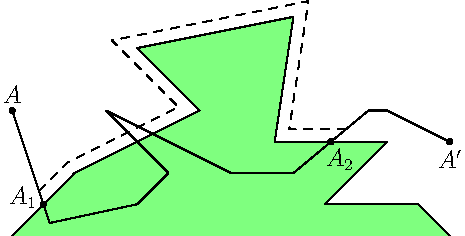
\includegraphics{jordan/navigation1.pdf}
\caption{Navigating around the Exterior}
\label{fig:Navigation1}
\end{figure}

\begin{figure}
\centering
\subfigure{\includegraphics{jordan/shorten1.pdf}\label{fig:Shorten1}}
\subfigure{\includegraphics{jordan/shorten2.pdf}\label{fig:Shorten2}}
\caption{Paths for IH3}
\end{figure}

\subsection{Union Case}
For the case depicted in Figure~\ref{fig:UnionCase}, we will assume, without loss of generality, that $Y$ lies in the interior of $p_1$ and $Z$ lies in the interior of $p_2$. We now define the interior of $p$ as the union of the interiors of $p_1$ and $p_2$ and the interior of the diagonal $PQ$. We define the exterior as the set of points not on the polygon and not in the interior. We just need to prove IH1--IH5 for the polygon $p$. 

\begin{description}
\item[IH1] Interior points $A$ and $B$ of $p$ can be connected by a polygonal path which does not intersect~$p$.
  \begin{proof}
    Suppose $A$ and $B$ both lie inside $p_1$, or both lie inside $p_2$. We apply IH1 to $p_1$ and $p_2$, and thereby connect $A$ and $B$ with a polygonal segment lying in the interior of $p$. On the other hand, if we suppose that $A$ is inside $p_1$ and $B$ is inside $p_2$, we apply IH1 to $p_1$ in order to connect $A$ to $Y$, and we apply IH1 to $p_2$ in order to connect $B$ to $Z$. The required path can then be completed with the segment $YZ$.
  \end{proof}
\item[IH2] Exterior points $A$ and $B$ of $p$ can be connected by a polygonal path which does not intersect $p$.
  \begin{proof}
    We must have that $A$ and $B$ lie in the exteriors of both $p_1$ and $p_2$. By IH2 applied to $p_1$, there is a path through the exterior of $p_1$ which connects $A$ and $B$. If this path lies entirely in the exterior of $p_2$ then it also lies entirely in the exterior of $p$ and we are done. 

    Otherwise, we take the first point $A_1$ and the last point $A_2$ at which the path crosses the boundary of $p_2$. We then find a new path which follows the edges of the polygon until it connects these two points. See Figure~\ref{fig:Navigation1} for an illustration and see \S\ref{sec:Jordan1NavigationDiscussion} for some discussion on this part of the proof.
  \end{proof}
\item[IH3] Any path connecting an interior point $A$ of $p$ to an exterior point $B$ of $p$, must intersect $p$.
  \begin{proof}
    Assume that $A$ lies in the interior of $p_1$ and $B$ lies in the exterior of both $p_1$ and $p_2$, and suppose there is a path connecting $A$ and $B$ which does not intersect $p$. By IH3 applied to $p_1$, this path must intersect the diagonal $PQ$. Take the last point at which it intersects this diagonal. Then there is a later point $A'$ on the path which we can connect to either $Y$ or $Z$ without crossing $PQ$. By IH5 applied to $p_1$ and $p_2$, it then follows that $A'$ is interior to either $p_1$ or $p_2$, whilst being connected to $B$. Hence, by IH3 applied to $p_1$ and $p_2$, the path must intersect $p$. See Figure~\ref{fig:Shorten1} for an illustration and see \S\ref{sec:Jordan1SameSideDiscussion} for further discussion.
  \end{proof}
\item[IH4] If $Y'$ and $Z'$ are endpoints of a segment which crosses exactly one side of $p$, then one point is interior while the other is exterior with respect to $p$.
  \begin{proof}
    Suppose $Y'Z'$ crosses a side of $p$. Then if we apply IH4 to $p_1$, we have that $Y'$ and $Z'$ lie in opposite regions with respect to $p_1$. Moreover, one of the points, say $Y'$, lies inside $p$. Aiming for a contradiction, we suppose that $Z'$ also lies inside $p$. Since it does not lie inside $p_1$, nor does it lie on $PQ$, it follows that it must lie inside $p_2$. But then if we apply IH5 to $p_2$, we find that $Y'Z'$ must cross a side of $p_2$. Hence, $Y'Z'$ crosses a side shared by both $p_1$ and $p_2$. This contradicts the fact that $p$ is simple and $PQ$ does not intersect either $p_1$ or $p_2$.
  \end{proof}
\item[IH5] If a segment $Y'Z'$ does not intersect $p$, then $Y'$ and $Z'$ lie in the same region.
  \begin{proof}
    If the segment does not intersect any side of $p$ and does not intersect any sides of $p_1$ or $p_2$, then the case reduces to IH5 applied to $p_1$ and $p_2$. If it does intersect $p_1$ or $p_2$, then the side intersected must be the diagonal $PQ$. In this case, we can find a path which does not intersect $p_1$ and which connects $Y$ to $Y'$, or a path which does not intersect $p_2$ and which connects $Y$ to $Z'$. Thus, $Y'$ is interior to one of $p_1$ and $p_2$ by IH5 and thus interior to $p$. The same argument applies to $Z'$. See \S\ref{sec:Jordan1SameSideDiscussion} for some further discussion. % Note that the above disjunction is a case-split on which side of $PQ$ the points $Y'$ and $Z'$ are on. I am confident that the step corresponds exactly to the use of same_side_wall_connected in the verified proof.
  \end{proof}
\end{description}

\subsection{Subtraction Case}
The second case differs from the first in that we lose the symmetry between $p_1$ and $p_2$. One of these polygon's interiors must be contained entirely by the other's. 

We can determine which by considering whether $P_1$ lies inside $p_2$ or whether $Q_1$ lies inside $p_1$. To see why these are alternatives, suppose that $P_1$ does not lie on $p_2$ (as depicted). Then it follows from IH5 and the fact that $p$ is simple that the boundary of $p_2 - PQ$ lies outside $p_1$. By considering a path interior to $p_2$ which connects $Z$ and $Q_1$, we can therefore conclude, again by IH5, that $Q_1$ must be interior to $p_1$. Again, see \S\ref{sec:Jordan1SameSideDiscussion} for further details.

We now assume, without loss of generality, that $Q_1$ is interior to $p_1$ as depicted. We then define the interior of $p$ to be the interior of $p_1$ minus the interior of $p_2$ and its boundary. 

Note that by IH5 and the fact that $p$ is simple, we have that all points on $p_2 - PQ$ must lie inside $p_1$, and that all points on $p_1 - PQ$ must lie outside $p_2$. We now prove IH1--IH5 for the step case.

\begin{description}
\item[IH1] Interior points $A$ and $B$ of $p$ can be connected by a polygonal path which does not intersect~$p$.
  \begin{proof}
    An interior point of $p$ is an interior point of $p_1$ which is not interior to $p_2$. If we apply IH1 to $p_1$, we can find a path between $A$ and $B$ through the interior of $p_1$. It is possible that this path intersects $p_2$, and so we must appeal to the same argument used for IH2 in the previous section and depicted in Figure~\ref{fig:Navigation1}, in order to navigate through the exterior of $p_2$.
  \end{proof}
\item[IH2] Exterior points $A$ and $B$ of $p$ can be connected by a polygonal path which does not intersect $p$.
  \begin{proof}
    This argument is similar to that given for IH1 in the previous section. If both $A$ and $B$ lie in the exterior of $p_1$, then we know from IH1 applied to $p_1$ that they can be connected by a path exterior to $p_1$. And since $p_2 - PQ$ is interior to $p_1$, we know that this path does not intersect $p$.

    Similarly, if $A$ and $B$ lie in the interior of $p_2$, we know from IH1 that they can be connected by a path interior to $p_2$. And since $p_1$ is not interior to $p_2$, we know that this path does not intersect $p$.

    Finally, if $A$ is exterior to $p_1$ and $B$ interior to $p_2$, then we can join $A$ to $Y$ by a path exterior to $p_1$ and $p_2$, and join $B$ to $Z$ by a path interior to $p_1$ and $p_2$. The segment $YZ$ then completes a path connecting $A$ to $B$ which does not intersect $p$.
    \end{proof}

\item[IH3] Any path connecting an interior point $A$ of $p$ to an exterior point $B$ of $p$, must intersect $p$.
  \begin{proof}
    The proof is similar to that for the previous section. By definition, $A$ lies inside $p_1$ and outside $p_2$. The point $B$, on the other hand, might lie inside $p_2$, outside $p_1$, or it might lie on the diagonal $PQ$. In any case, we can conclude that the path intersects the diagonal $PQ$, by applying IH3 to one of $p_1$ and $p_2$. We now take the first point at which the path intersects the diagonal. Then there will be an earlier point $A'$ on the path which must either lie outside $p_1$ or lie inside $p_2$. This point is connected to $A$ by a path which does not intersect $PQ$, and thus, by applying IH3 to one of $p_1$ and $p_2$, we can find a point where the path intersects $p$. See Figure~\ref{fig:Shorten2} for an illustration.
  \end{proof}

\item[IH4] If $Y'$ and $Z'$ are endpoints of a segment which crosses exactly one side of $p$, then they lie in different regions with respect to $p$.
  \begin{proof}
     Suppose that $Y'Z'$ intersects a side of $p_1$. If we apply IH4 to $p_1$, we find that one of these points must be interior to $p_1$ and the other exterior. Moreover, since the point of intersection of $Y'Z'$ with $p_1$ is exterior to $p_2$, we can apply IH5 to $p_2$ and conclude that $Y'$ and $Z'$ are both exterior to $p_2$. It follows by the definition of $p$ that $Y'$ and $Z'$ are then in opposite regions. A similar argument applies if $Y'Z'$ intersects a side of $p_2$.
  \end{proof}
\item[IH5] If a segment $Y'Z'$ does not intersect $p$, then $Y'$ and $Z'$ lie in the same region.
  \begin{proof}
    If $Y'Z'$ does not intersect $p_1$ or $p_2$, then this reduces to the case IH5 applied to these polygons. Otherwise, we suppose that $Y'Z'$ intersects the diagonal $PQ$. 

    If $Y'$ is inside $p$, then it lies inside $p_1$ and outside $p_2$, and thus $Z'$ must be outside $p_1$ by IH4 applied to $p_1$. But this means that both $Y'$ and $Z'$ lie outside $p_2$, which contradicts IH5 applied to $p_2$. 

    On the other hand, if $Y'$ is not inside $p$, then there are two possibilities for its location:
    \begin{description}
    \item[The point $Y'$ lies inside $p_1$ and $p_2$] In this case, we can apply IH4 to $p_2$ and conclude that $Z'$ is outside $p_2$. By definition, both points are then exterior to $p$. 
    \item[The point $Y'$ lies on $PQ$] In this case, $Z'$ must also lie on $PQ$. Again by definition, both points are then exterior to $p$.
    \item[The point $Y'$ lies outside both $p_1$ and $p_2$] Here, we apply IH4 to the point $p_2$, and thus conclude that the point $Z'$ is inside $p_2$. By definition, both points are then exterior to $p$.
    \end{description}
  \end{proof}
\end{description}

\subsection{Discussion}
There are a few definite gaps in this first proof attempt. As said, we neglected to prove the base case for triangles, and we have not shown that the recursively defined interiors and exteriors are always non-empty. Finally, the without-loss-of-generality assumption made in finding the diagonal of a polygon needs to be carefully justified (it amounts to showing that a polygon cannot have a spiral shape).
 We consider these to be fairly straightforward matters, however. 

This is not the proof we chose to verify, though the one we \emph{have} verified shares many of its inferences. When we come to verify those inferences, we shall see that many details above have been glossed over. We hope, then, to convince the reader to be quite wary of the above proof as it stands. The details that we have glossed over will be put on a more solid footing when we discuss our formal verification.

\label{sec:Jordan1NavigationDiscussion}For instance, in Figure~\ref{fig:Navigation1}, we claim to be able to navigate around the exterior of a simple polygon. This intuitive idea will be needed again in our verified proof, where it needs to be carefully formulated, and the formulation needs to be carefully tied back to the premises and the desired conclusion. The details are given in \S\ref{sec:NavigationProof}.

\label{sec:Jordan1SameSideDiscussion}At several places in the above proof, we also assumed we could always find a path connecting the points $Y$ and $Z$ in Figures~\ref{fig:UnionCase} and~\ref{fig:SubCase} to various other points. A careful formulation of what characterises such points, together with a proof that the required path can be exhibited, is given in \S\ref{sec:JordanSameSideProof}.

We have retained the above proof because of its computational properties. It recursively \emph{builds} the interior of a polygon from the interiors of triangles, and thus describes the algorithm for a point-in-polygon test by reducing the problem to point-in-triangle tests, which, in turn, reduce to point in half-plane tests. Our \emph{verified} proof does not have this feature. It was inspired by Veblen's proof, and its basic structure and focus are very different. Nevertheless, it is interesting that a number of the key steps overlap, and we shall refer back to this proof when we discuss the verification of the polygonal Jordan Curve Theorem in Chapter~\ref{chapter:JordanVerification}.

\section{Veblen's Proof}\label{sec:VeblenProof}
In his 1904 doctoral thesis~\cite{Veblenphd}, Veblen set out a basic set of axioms for Euclidean Geometry. His incidence and order axioms are very similar to Hilbert's own, and it is not difficult to prove their equivalence. Unlike Hilbert, he provided a complete proof for the polygonal Jordan Curve Theorem, and we shall discuss that proof in this section, comparing it to the one we sketched in \S\ref{sec:JordanCurveFirstProof}.

Veblen does not explicitly define the interior or exterior of a polygon. Like most other proofs, he tries to show that the two regions exist implicitly by dividing the theorem into two claims: the first states that a simple polygon divides its plane into at least two regions; the second states that the polygon divides its plane into at most two regions. Both assertions can be formalised directly in terms of points and 

\begin{enumerate}
\item there are at least two points in the plane not on $p$ which cannot be connected by a polygonal segment without crossing $p$\label{list:VeblenLemma1};
\item of any three points in the plane not on $p$, at least two of them can be connected by a polygonal segment without crossing $p$.
\end{enumerate}

We will point out in advance that Veblen's proof is a two page proof and one of the most detailed in his thesis. This again brings into question Hilbert's claim that the theorem can be easily derived. We might also consider the fact that Hilbert was willing to give explicit proofs of much simpler theorems, such as his Theorem~3 (see \S\ref{sec:Theorem3}). 

Furthermore, it is questionable whether Veblen's proof is even correct. According to Reeken and Kanovei~\cite{HahnInconclusiveIndirect}, the proof was deemed ``inconclusive'' by Hahn, while Guggenheimer claims, citing Lennes and Hahn, that Veblen's proof assumes that a polygon can be triangulated and is otherwise only valid for convex polygons~\cite{GuggenheimerJordanCurve}. We could not find this criticism in Lennes~\cite{LennesPolygon}, and were initially satisfied by Veblen's proof, and so we attempted a verification of assertion (\ref{list:VeblenLemma1}) above. Eventually, as one might expect, we hit an obstacle. In the next few sections, we will try to explain the difficulty.

\subsection{Veblen's Lemma 1}\label{sec:VeblenLemma1}
The first half of Veblen's proof is given as the corollary to a very general theorem about polygons, expressed in terms of ``multiple points'', which are those points, should they exist, where a polygonal self-intersects:
\begin{quote}
Lemma 1. \emph{If a side of a polygon $q$ intersects a side of a polygon $p_n$ in a single point $O$ not a multiple point of $p_n$ or $q$, then $p_n$ and $q$, whether simple or not, have at least one other point in common.} 
\end{quote}

We can highlight the generality of this theorem by considering a particularly degenerate version of polygons. Consider the example in Figure~\ref{fig:jordanDegenerate1}. Here, we have two polygons $P_1P_2P_3$ and $Q_1Q_2Q_3$. The points of these polygons are obviously collinear and so cannot divide the plane into multiple regions. But neither are they a counterexample to Veblen's lemma, since their point of intersection $X$ is a multiple point of both, lying simultaneously on the segments $P_1P_2$ and $P_2P_3$, and also lying on the segments $Q_1Q_2$ and $Q_2Q_3$.

\begin{figure}
\centering
\includegraphics{jordan/jordanDegenerate1}
\caption{Degenerate polygons intersecting at a multiple point}
\label{fig:jordanDegenerate1}
\end{figure}

We have formally verified that this particular lemma follows from Hilbert's axioms (see \S\ref{sec:Lemma1Verification}), but we gave up trying to reproduce Veblen's argument, and believe it to be invalid. We do not have a counterexample, as such, since we do not think Veblen's proof is sufficiently detailed to say exactly where it fails. Instead, we have tried to illustrate the difficulties we faced with the example in Figure~\ref{fig:VeblenCounter1}. This example shows a simple maze polygon $p_n$ being intersected at a point $O$ by another polygon $q$ shown in red. The goal is to identify one of the other seven points of intersection. Our labelling in the diagram is consistent with the set-up to Veblen's proof:

\begin{quote}
If $n=3$ ($q$ having any number of sides, $m$) the theorem reduces to [the case for triangles]. We assume without loss of generality that no three vertices $P_{i-1}$, $P_i$, $P_{i+1}$ are collinear and prove the lemma for every $n$ by reducing to the case $n=3$. Let $p_n$ have $n$ vertices with the notation such that the side $P_1P_2$ meets $q$ in the side $Q_1'Q_2'$ where the segment $Q_2'O$ contains no interior point of the triangle $P_1P_2P_3$.\end{quote}

\begin{figure}
\centering
\includegraphics[scale=0.6]{jordan/veblenCounter1.pdf}
\caption{Intersections on a simple maze}
\label{fig:VeblenCounter1}
\end{figure}

Veblen's basic strategy is to consider each of the triangles $P_1P_2P_3$, $P_1P_3P_4$, $P_1P_4P_5$, $P_1P_5P_6$, $\ldots$. Of these triangles, all but the first and last share exactly one side with the polygon $p_n$, with the other sides being diagonals of the polygon. Veblen tries to show that if $q$ intersects one of these triangles in one diagonal, then it intersects the next triangle. In this way, intersections can be found, one after the other, down the list of triangles, until we eventually find a second point of intersection with the polygon $p_n$.

\subsection{Finding a subset of $q$}\label{sec:SubsetOfQ}
In Figure~\ref{fig:VeblenCounter2}, we show a polygonal segment  (or ``broken line'') which is a subset of the polygon $q$, with vertices $O_kQ_2'Q_3'Q_4'Q_5'Q_6'O_j$. This segment makes contact with the diagonal $P_1P_3$ exactly twice, once from the outside of the triangle $P_1P_2P_3$, and once from the inside. The polygonal segment always exist, and can be proven to intersect $P_1P_3$ in just this way. To find it, we start from the segment $Q_2'Q_3'$ and progressively add neighbouring segments until we eventually reach a segment which intersects the line $P_1P_3$. As Veblen puts it:

\begin{figure}
\centering
\includegraphics[scale=0.6]{jordan/veblenCounter2.pdf}
\caption{A chosen subset of $q$: $k=2$ and $j=6$}
\label{fig:VeblenCounter2}
\end{figure}

\begin{quote}By the case $n=3$, $q$ meets the boundary of the triangle $P_1P_2P_3$ in at least one point other than $O$. If this point is on the broken line $P_1P_2P_3$ the lemma is verified. If not, $q$ has at least one point on $P_1P_3$, and at least one of the segments $Q_1'Q_2'$, $Q_2'Q_3'$ has no point or end-point on $P_1P_3$. Let this segment be one segment of a broken line $Q_kQ_{k+1}\cdots Q_{j-1}Q_j$ of segments of $q$ not meeting $P_1P_3$ but such that $Q_{k-1}Q_k$ and $Q_jQ_{j+1}$ do each have a point or endpoint in common with $P_1P_3$ ($1 \leq k < j \leq m$; if $k = 1$, $Q_{k-1} = Q_m$; if $j = m$, $Q_{j+1} = Q_1$). If $O_j$ is the point common to $P_1P_3$ and $Q_jQ_{j+1}$ or $Q_{j+1}$, and $O_k$ is the point common to $P_1P_3$ and $Q_{k-1}Q_k$ or $Q_{k-1}$, the broken line $O_kQ_kQ_{k+1}\cdots Q_{j-1}Q_jO_j$, has a point inside and also a point outside the triangle $P_1P_2P_3$ and cuts the broken line $P_1P_2P_3$ only once. \end{quote}

Now there is nothing particularly informative about Veblen's last remark. Notice that the segment $Q_1'Q_2'$ \emph{also} has a point inside and a point outside the triangle $P_1P_2P_3$. It also cuts the polygonal segment $P_1P_2P_3$ exactly once. Something is missing here. There must be some other property had by the polygonal segment $O_kQ_kQ_{k+1}\cdots Q_{j-1}Q_jO_j$, in order for Veblen to get to his very next claim, that ``it has a point inside and a point outside any triangle of which $P_1P_3$ is a side''. The missing property is an important detail, because as we mentioned, part of the argument is supposed to be repeated down the list of triangle $\triangle P_1P_2P_3$, $\triangle P_1P_3P_4$, $\triangle P_1P_4P_5$, $\triangle P_1P_5P_6$, $\ldots$. If we are going to repeat this part of the argument, we need to know that any missing properties will be valid in the repeated case.

For now, we just note that Veblen's claim certainly follows. The crucial point is that, as we remarked earlier, the polygonal segment $O_kQ_kQ_{k+1}\cdots Q_{j-1}Q_jO_j$ touches $P_1P_3$ exactly twice, once from the outside and once from the inside. More precisely, we just note that the interior of $Q_kO_k$ is outside the triangle, while the interior of $Q_jO_j$ is inside. To establish this, we note that the points inside the segment $O_kO$ are all inside the triangle $P_1P_2P_3$~\footnote{For Veblen, this is a matter of definition. See ~\ref{sec:triangleDef}}. Thus, by the Jordan Curve Theorem applied to triangles, all points of the polygonal segment $O\cdots O_{j-1}O_j$ must be outside the triangle $P_1P_2P_3$. It is then possible to show that the points inside the segment $O_kO$ are on the opposite side of the line $P_1P_3$ as the points inside the segment $Q_{j-1}O_j$, and so must be in different regions of any triangle of which $P_1P_3$ is a side. Veblen's claim then follows: the polygonal segment $O_kQ_kQ_{k+1}\cdots Q_{j-1}Q_jO_j$ has a point inside and a point outside any triangle of which $P_1P_3$ is a side. We just needed a bit of extra work to get there.

\subsection{Veblen's Conclusion}
\begin{quote}On this account if $P_1P_3P_4$ are not collinear, and obviously, if $P_1P_3P_4$ are collinear, $q$ must meet either $P_3P_4$ or $P_4$ or $P_4P_1$. If $q$ does not meet $P_3P_4$ or $P_4$, we proceed with $P_1P_4P_5$ as we did with $P_1P_3P_4$. Continuing this process, we either verify the lemma or come by $n-2$ steps to the triangle $P_1P_{n-1}P_n$ and find that $q$ must intersect the broken line $P_{n-1}P_nP_1$, which also verifies the lemma.\end{quote}

This is Veblen's conclusion, and the situation described is illustrated in Figure~\ref{fig:VeblenCounter3}. The first step follows by the Jordan Curve Theorem applied to triangles: we know that $O_kQ_kQ_{k+1}\cdots Q_{j-1}Q_jO_j$ does not strictly\footnote{The use of phrases such as ``strictly cut'', among many other details, will be clarified in our verification. See Chapter~\ref{chapter:JordanVerification}.} \emph{cut} the line $P_1P_3$, so it must instead cut either $P_1P_4$ or $P_3P_4$. We can assume that $q$ does not meet $P_3P_4$, and so we proceed with $P_1P_4P_5$. But Veblen is not clear on exactly \emph{how} the argument repeats. The reason the first step follows in the above conclusion is because $O_kQ_kQ_{k+1}\cdots Q_{j-1}Q_jO_j$ does not cut $P_1P_3$, but we have now assumed that it \emph{does} cut $P_1P_4$, so we are not simply repeating the conclusion. 

\begin{figure}
\centering
\includegraphics[scale=0.6]{jordan/veblenCounter3.pdf}
\caption{Intersections with $P_1P_3P_4$}
\label{fig:VeblenCounter3}
\end{figure}

Notice that in this conclusion, Veblen has slipped to talking about the original polygon $q$ rather than the polygonal segment $O_kQ_kQ_{k+1}\cdots Q_{j-1}Q_jO_j$ which is a subset of $q$. Presumably then, we need to find another subset of $q$ which has the same properties as the original. And here we encounter the problem of detail mentioned at the end of \S\ref{sec:SubsetOfQ}: we were not sure to begin with what the crucial properties of the subset \emph{are}. Nevertheless, we tried earlier to fill in those details, and based on our attempt, we might assume that the desired polygonal segment for our example is the one shown in Figure~\ref{fig:VeblenCounter4}, namely $O_k'O_kQ_2'Q_3'Q_4'O_j'$. This polygonal segment can be identified by starting at the point $O_k$ and following Veblen's procedure as we did with the point $O$. 

\begin{figure}
\centering
\includegraphics[scale=0.6]{jordan/veblenCounter4.pdf}
\caption{Desired subset of $q$?}
\label{fig:VeblenCounter4}
\end{figure}

Remember that Veblen's next claim is that the polygonal segment $O_k'O_kQ_2'Q_3'Q_4'O_j'$ has a point inside and outside any triangle of which $P_1P_3$ is a side. Again, this is certainly true. But earlier, we justified it by noting that the polygonal segment touches $P_1P_4$ exactly twice, once from inside the triangle and once from outside. More formally, we can notice that the points inside the segment $O_k'Q$ lie inside the triangle $P_1P_3P_4$, while the points inside the segment $Q_4'O_j'$ lie outside the triangle. We could establish this earlier by relying on Veblen's assertion that the polygonal segment $O_k'O_kQ_2'Q_3'Q_4'O_j'$ crosses $P_1P_3$ \emph{exactly once}, but this is no longer true. Instead, the required observation is that it crosses $P_1P_3$ an \emph{odd} number of times, and so it has a non-empty suffix which lies entirely outside the polygon. 

We therefore need a proof that the number of crossings must always be odd, but we cannot see anything in Veblen's argument that would require this. We presumably need additional lemmas about the parity of crossings on a triangle's side. But as soon as we start to do \emph{that}, we can immediately identify an argument which is conceptually much more straightforward. We give this argument in full in \S\ref{sec:ParityProofInformal}.

\section{Conclusion}
In this chapter, we have looked at several proofs of the Jordan Curve Theorem for simple polygons which might be applicable to Hilbert's two groups of axioms. Our first proof started with a recursive definition of an arbitrary polygon's interior and exterior. It explained how to add and subtract smaller polygons at each recursive step until we arrive at the base-case in triangles. The rest of the proof then shows that the recursive definition always yields two distinct regions which cover the plane, and such that any two points in the regions can be joined by a polygonal segment.

We then reviewed Veblen's 1904 proof of the theorem, from axioms equivalent to Hilbert's, and which, on the face of it, is far simpler to our first proof. However, it has been claimed elsewhere~\cite{GuggenheimerJordanCurve,HahnInconclusiveIndirect} to be invalid. Based on a verification attempt, we believe we have identified the crucial problem, and have suggested that its fix leads immediately to a conceptually simple parity proof. In the next chapter, where we shall review our verification of the parity proof, we shall be able to constrast its conceptual simplicity with the complexity of its details. 

With the verification, we have now unquestionably shown that despite the seeming theoretical poverty of Hilbert's first two groups, we have sufficient primitives and axioms to prove the Jordan Curve Theorem for polygons. We also hope that our analysis of the proof shows that Hilbert was mistaken to think the theorem could be obtained ``without serious difficulty.''

%%% Local Variables: 
%%% TeX-master: "../thesis"
%%% End: 

\chapter{Formalising the Polygonal Jordan Curve Theorem}\label{chapter:JordanFormalisation}
% In this chapter, we will analyse our HOL~Light~\cite{HOLLight} verification of the Jordan Curve Theorem for Polygons. This theorem appears as Theorem~9 in the 10th edition of Hilbert's \emph{Grundlagen der Geometrie}. The verification might stand on its own: the theorem's formulation does not appeal to earlier definitions or theorems, and of all the proofs we have considered, its verification is the most complicated by an order of magnitude. But the theorem also serves as a useful case-study for the tools that we have developed up to this point: the linear reasoning tactic from Chapter~\ref{chapter:LinearOrder} was used pervasively in verifying the theorem, becoming the crucial work-horse for solving and exploring complex linear ordering problems. We leveraged the theory of Half-Planes from Chapter~\ref{chapter:HalfPlanes} as the basis for key lemmas on two-dimensional ordering. Lastly, the discovery algebra described in Chapter~\ref{chapter:Automation} was needed throughout to verify incidence problems and to identify case-splits and suggest proof strategies based on discovered facts. 

In this chapter, we introduce our verification of the Polygonal Jordan Curve Theorem, and we present its formalisation in full. We will set forth, unambiguously, \emph{what} we have verified, and thus, much of this chapter can be read independently of the verification. The formal definitions and formalisations are not as simple as those in earlier chapters, and so they must be carefully checked. But once we are convinced that the formalisations correctly capture the statement of the theorem, we have an absolute guarantee that it is derivable from Hilbert's axioms.

\section{Organisation}
The verification is divided neatly into two parts, corresponding to the verification of two theorems, which we formalise in \S\ref{sec:JordanFormulation}:
\begin{enumerate}
  \item there are two points in the plane of a simple polygon such that any polygonal path connecting them must cross the simple polygon (verified in Chapter~\ref{chapter:JordanVerification1});
  \item given three points in the plane of a simple polygon, there is a polygonal path connecting two of those points (verified in Chapter~\ref{chapter:JordanVerification2}).
\end{enumerate}

When we discuss the verifications, we will use the same basic structure. First, we shall give an overview of the theory structure, effectively amounting to a sketch proof of the theorem. From this, we shall give formalisations of any key concepts mentioned in the proof. In the case of the first part of the Polygonal Jordan Theorem, these are the concepts of triangle interiors and exteriors and the concept of a ``crossing'' of a triangle by a polygonal path. For the second part of the theorem, we have concepts of ``lines-of-sight'' and polygon rotations. 

These concepts are supported by a suite of lemmas. Consistent with the synthetic style of geometric proof, these lemmas generally break down into one of two forms. We have lemmas which introduce points and other objects in a geometrical configuration. We also have lemmas which allow us to infer properties of these configurations. The two sorts of lemmas are used in tandem: we build up complex figures using the ``introduction'' rules, and then use the other rules to satisfy the hypotheses of yet more ``introduction'' rules, and so on. Many of these lemmas are interesting in their own right, and we shall pick a few for closer examination.

We present some extracts of what we hope are interesting verifications, ones which highlight the benefits and drawbacks of our representations in terms of the resulting proof mechanics. We hope to use these extracts to convince the reader that we have stayed faithful to the synthetic style of proof, even as the verifications grow significantly in complexity. The complexity is easy enough to measure. The verifications from Chapter~\ref{chapter:Group2Eval} take only a dozen or so steps. The verifications in the next few chapters frequently run to hundreds, and we suspect this really is due to the complexity of the synthetic reasoning involved.

\section{Related Work}
The Jordan Curve Theorem has some notoriety within the formal verification community, and has long been regarded as a major milestone, one which  demonstrates the feasibility of formal verification on non-trivial mathematics problems. The MIZAR~\cite{MizarMathematicalVernacular} community first began a verification in 1991, and completed the special case for polygons in 1996. The full proof was completed in 2005. In the same year, Hales completed an independent proof in HOL~Light~\cite{HalesJordanCurve}. 

Both proofs use the special case for polygons as a lemma, though in a restricted form: in the case of the MIZAR proof, only polygons with edges parallel to axes are considered. In Hales' proof, the polygon is restricted to lie on a grid. Moreover, the formulations are algebraic rather than synthetic, and so are outside the scope of Hilbert's and Veblen's formulations.

In 2009, Dufourd~\cite{DufourdJordanCurve} formally verified a constructive proof of the Discrete Jordan Curve Theorem. This theorem characterises Jordan curves in terms of a ``ring'' of faces in a subdivision of a plane or sphere. This is a more practical achievement, since we can expect this sort of characterisation to be more useful to computer scientists trying to express and reason about topological properties computationally. However, our interest here is in Hilbert's formulation and a synthetic proof of the Jordan Curve Theorem in ordered geometry.

%\section{Foundational Issues}
% Many of Hilbert's definitions and theorems are first-order logic, and indeed, much of our formalisation makes no essential use of higher-order or number theoretical notions. But as with Hilbert`s Theorem~6 which we discussed in \S\ref{sec:Theorem6}, things are not so clear for Hilbert's definition of polygons.

% It seems easy to excuse Hilbert's lack of clarity on these matters, since he was working before symbolic first-order logic had been invented. But then, when we consider the reviews by Veblen and Poincar\'{e}~\cite{VeblenHilbertReview,PoincareReview}, we realise that the community was certainly interested in the mechanisation of logic. Both reviews anticipate the mechanical verification of Hilbert's geometry, and both mention the work of Peano, whose formulations of logic and mathematics were higher-order, and even admitted recursive definitions. Peano's ideas would later be developed in Russell's \emph{Principles of Mathematics}~\cite{PrinciplesOfMathematics}, which led directly to Russell and Whitehead's \emph{Principia Mathematica}.

% We realise there is some controversy about how strong the logic should   , we have not been shy about using 

% \begin{quote}[The axioms] presuppose only the validity of the operations of logic and counting (ordinal number).\end{quote}

% As with Hilbert's Theorem~6 \S\ref{sec:Theorem6}, a formulation of polygon and polygonal path raises a number of questions relating to our logical foundations. As we have previously stated, Hilbert's work predates the systematic development of first-order logic, and 

\section{Formulation}\label{sec:JordanFormulation}
\begin{quotation}
  DEFINITION. A set of segments $AB$, $BC$, $CD$, $\ldots$, $KL$ is called a \emph{polygonal segment} that connects the points $A$ and $L$. Such a polygonal segment will also be briefly denoted by $ABCD\ldots KL$. The points inside the segments $AB$, $BC$, $CD$, $\ldots$, $KL$ as well as the points $A$, $B$, $C$, $D$, $\ldots$, $K$, as well as the points $A$, $B$, $C$, $D$, $\ldots$, $K$, $L$ are collectively called the \emph{points of the polygonal segment}. 

In addition, for a polygonal segment $A$, $B$, $C$, $\ldots$, $L$, we shall call the segments $AB$, $BC$, $CD$, $\dots$, $KL$ the \emph{sides} of the polygonal segment.
\flushright{\emph{Foundations of Geometry}~\cite{FoundationsOfGeometry} (page 8)}
\end{quotation}
This is Hilbert's first key definition, defining what Veblen calls \emph{broken lines}, and what we shall prefer to call \emph{polygonal paths}. Contrary to his conventions~(see \S\ref{sec:DistinctVars}), Hilbert does not insist that the points involved here are distinct. Indeed, he adds an explicit distinctness clause when he defines simple polygons (see \S\ref{sec:polygonFormalisation}).

One thing which is clear to us is that Hilbert's notation is doing the heavy lifting in this definition. He uses it to take care of the otherwise clumsy constraint that all but two segments in the set share their endpoints with at least two other segments. The remaining two elements must share exactly one of their endpoints with another segment.

Had Hilbert given a proof of the polygonal Jordan Curve Theorem, he would have probably used his notation to do more heavy lifting, as Veblen did in his own proof. Veblen's argument ends up running over symbols and numerical subscripts in a way which seems to take us out of the world of synthetic geometry, and back into the sort of computational metatheory we saw in \ref{eq:six} from Chapter~\ref{chapter:LinearOrder}.
\begin{quotation}
  By the case $n=3$, $q$ meets the boundary of the triangle $P_1P_2P_3$ in at least one point other than $O$. If this point is on the broken line $P_1P_2P_3$ the lemma is verified. If not, $q$ has at least one point on $P_1P_3$, and at least one of the segments $Q_1'Q_2'$, $Q_2'Q_3'$ has no point or end-point on $P_1P_3$. Let this segment be one segment of a broken line $Q_kQ_{k+1}\cdots Q_{j-1}Q_j$ of segments of $q$ not meeting $P_1P_3$ but such that $Q_{k-1}Q_k$ and $Q_jQ_{j+1}$ do each have a point or endpoint in common with $P_1P_3$ ($1 \leq k < j \leq m$; if $k = 1$, $Q_{k-1} = Q_m$; if $j = m$, $Q_{j+1} = Q_1$). If $O_j$ is the point common to $P_1P_3$ and $Q_jQ_{j+1}$ or $Q_{j+1}$, and $O_k$ is the point common to $P_1P_3$ and $Q_{k-1}Q_k$ or $Q_{k-1}$, the broken line $O_kQ_kQ_{k+1}\cdots Q_{j-1}Q_jO_j$, has a point inside and also a point outside the triangle $P_1P_2P_3$ and cuts the broken line $P_1P_2P_3$ only once.
\flushright{Veblen~\cite{Veblenphd} (page~365)}
\end{quotation}
Looking at Veblen's proof attempt, one might expect the argument to be dominated by computations and lemmas about point sequences, and not by synthetic constructions of diagrams, but this is not entirely the case. Our verification shows that there are a \emph{lot} of useful lemmas very similar to those we saw in Chapter~\ref{chapter:Group2Eval}, whose synthetic proofs obtain and then reason about properties of diagrams.

% Metatheoretical arguments like this go at least back to Euclid. Consider Euclid's classic Proposition 20 from Book IX:
% \begin{quote}
% Prime numbers are more than any assigned multitude of prime numbers.
% Let $A$, $B$, and $C$ be the assigned prime numbers.

% I say that there are more prime numbers than $A$, $B$, and $C$.
% \end{quote}
% This is not a proof, but more like a proof \emph{template}. Euclid is assuming his reader knows how to repeat the argument for other assignments of prime numbers besides $A$, $B$ and $C$!

% This is fairly typical of prose mathematics, where the notation itself because the means to establish constraints and the mechanism of reasoning. Consider again, Veblen's proof from the last chapter, to see how mathematical proofs can involve complicated arguments, not about the mathematical objects of the theory, but the \emph{symbols} used to denote them:

% \begin{quote}Let this segment be one segment of a broken line $Q_kQ_{k+1}\cdots Q_{j-1}Q_j$ of segments of $q$ not meeting $P_1P_3$ but such that $Q_{k-1}Q_k$ and $Q_jQ_{j+1}$ do each have a point or endpoint in common with $P_1P_3$ ($1 \leq k < j \leq m$; if $k = 1$, $Q_{k-1} = Q_m$; if $j = m$, $Q_{j+1} = Q_1$). If $O_j$ is the point common to $P_1P_3$ and $Q_jQ_{j+1}$ or $Q_{j+1}$, and $O_k$ is the point common to $P_1P_3$ and $Q_{k-1}Q_k$ or $Q_{k-1}$, the broken line $O_kQ_kQ_{k+1}\cdots Q_{j-1}Q_jO_j$, has a point inside and also a point outside the triangle $P_1P_2P_3$ and cuts the broken line $P_1P_2P_3$ only once.\end{quote}

%As we described Hilbert's Theorem~6 (see \S\ref{sec:Theorem6}) as a metatheorem, we would describe Veblen's argument here as a \emph{metaproof}. The use of such metatheoretical arguments in axiomatic geometry probably goes back to Euclid, who 

With the notation doing such heavy lifting, we will formalise it directly. We opted to represent polygonal paths as their finite sequence of points, from which the original polygonal paths can be recovered. With this definition, the clumsy constraint about segments sharing endpoints is handled implicitly. The heavy lifting will be carried out as computations on lists, which are available to us in the logic, ultimately being defined in terms of natural numbers. As we saw in Chapter~\ref{chapter:LinearOrder}, this means they are still ultimately represented by geometric figures. 

%TODO: Discuss or refer to an earlier discussion about using lists to handle ``meta-level'' definitions, and why lists are somewhat justified by the fact that all infinite structures are now abstractions over geometric objects since we have derived the axiom of infinity.

Now the list library in HOL Light is slightly impoverished (at least compared with, say, that of Isabelle/HOL), and so our verification had to take a detour as we added new function definitions and theorems for lists. For instance, in order to recover the edges of a polygonal path, we must take adjacent pairs of the points in its vertex list. We can do this by following a standard pattern in functional programming, shown in Figure~\ref{fig:AdjacentSpec}. The function \code{adjacent} zips all but the last element of a list with its tail. However, it is generally easier and requires much less unfolding to compute directly with the recursive specification of the function. We give this along with the definitions and specifications of other auxiliary functions in Figure~\ref{fig:ListDefinitions}.

\begin{figure}
\begin{align*}
  &\code{adjacent}\; : \; [\alpha] \rightarrow [(\alpha,\alpha)]\\
  \vdash_{def}\;&\code{adjacent}\ [P_0,P_1,P_2,\ldots,P_n]\\
  &\quad=\code{zip}\ (\code{butlast}\ [P_0,P_1,P_2,\ldots,P_n])\ (\code{tail}\ [P_0,P_1,P_,2,\ldots,P_n])\\
  &\quad= \code{zip}\ \begin{array}[t]{rcccccl}\lbrack & P_0,&P_1,&P_2,&\ldots,&P_{n-1}&\rbrack\\
    \lbrack & P_1,&P_2,&P_3,&\ldots,&P_n&\rbrack
  \end{array}\\
  &\quad= [(P_0,P_1),(P_1,P_2),(P_2,P_3),\ldots,(P_{n-1},P_n)]\\\\
  &\vdash\code{adjacent}\ [] = []\\
  &\vdash\code{adjacent}\ [x] = []\\
  &\vdash\code{adjacent}\ (\cons{x}{\cons{y}{xs}}) = \cons{(x,y)}{\code{adjacent}\ (\cons{y}{xs})}
\end{align*}
\caption{Specifications for $\code{adjacent}$}
\label{fig:AdjacentSpec}
\end{figure}

\begin{figure}
\begin{alignat*}{3}
  & \code{head}\,:\,[\alpha] \rightarrow \alpha &\qquad
  & \code{tail}\,:\,[\alpha] \rightarrow [\alpha]\dag &\qquad
  & \code{length}\ [\alpha]\rightarrow \mathbb{N}\\
  \vdash_{def}\;& \code{head}\ (\cons{x}{xs}) = x &\qquad
  \vdash_{def}\;& \code{tail}\ [] = [] &\qquad
  \vdash_{def}\;& \code{length}\ [] = 0\\
  & &\qquad
  \vdash_{def}\;&\code{tail}\ (\cons{x}{xs}) = xs &\qquad
  \vdash_{def}\;& \code{length}\ (\cons{x}{xs})\\
  & & & & &\quad = \code{length}\ xs + 1
\end{alignat*}
\begin{align*}
  &\code{butlast}\,:\,[\alpha] \rightarrow [\alpha]\\
  \vdash_{def}\;&\code{butlast}\ [] = []\\
  \vdash_{def}\;&\code{butlast}\ (\cons{x}{xs}) = \code{if}\ xs=[]\ \code{then}\ []\ \code{else}\ \cons{x}{(\code{butlast}\ xs)}
\end{align*}
\begin{align*}
  &\code{el}\,:\,\code{int} \rightarrow [\alpha] \rightarrow \alpha\\
  \vdash_{def}\;&\code{el}\ 0\ xs = \code{head}\ xs\\
  \vdash_{def}\;&\code{el}\ (\code{suc}\ n)\ xs = \code{el}\ n\ (\code{tail}\ xs)
\end{align*}
\begin{align*}
  & \code{mem}\,:\,\alpha \rightarrow [\alpha] \rightarrow \code{bool} &\qquad
  & \code{all}\,:\,(\alpha\rightarrow\code{bool}) \rightarrow [\alpha] \rightarrow \code{bool}\\
  \vdash_{def}\;& \code{mem}\ x\ [] = \bot &\qquad
  \vdash_{def}\;& \code{all}\ p\ [] = \top\\
  \vdash_{def}\;& \code{mem}\ x\ (\cons{y}{ys}) = x = y \vee \code{mem}\ x\ ys &\qquad
  \vdash_{def}\;& \code{all}\ p\ (\cons{x}{xs}) = p\ x \wedge \code{all}\ p\ xs   
\end{align*}
\begin{align*}
  & \code{pairwise}\,:\,(\alpha \rightarrow \alpha \rightarrow \code{bool}) \rightarrow [\alpha] \rightarrow \code{bool}\\
  \vdash_{def}\;& \code{pairwise}\ R\ [] = \top\\
  \vdash_{def}\;& \code{pairwise}\ R\ (\cons{x}{xs}) = \code{all}\ (R\ x)\ xs \wedge \code{pairwise}\ R\ xs
\end{align*}
\begin{align*}
  & \code{disjoint}\,:\,(\alpha\rightarrow\code{bool})\rightarrow(\alpha\rightarrow\code{bool})\rightarrow\code{bool}\\
  \vdash_{def}\;& \code{disjoint}\ S\ T = S \cap T = \emptyset
\end{align*}
$\dag$ This function is a more well-defined version of the existing function in HOL~Light. The original version is undefined for the empty list.
\caption{List definitions and specifications}
\label{fig:ListDefinitions}
\end{figure}

With the function $\code{adjacent}$, we can define the points of a polygonal path. As per Hilbert's definition, these are the points of the vertex list and the points inside each individual segment $(x,y)$. We can test for each using the list-membership predicate~$\code{mem}$.
\begin{equation}\label{eq:OnPolyPath}
  \begin{split}
    &\code{on\_polypath}\,:\,[\code{point}] \rightarrow \code{point} \rightarrow \code{bool}\\
    \vdash_{def}\;&\code{on\_polypath}\ Ps\ P \iff \\
    &\quad\code{mem}\ P\ Ps\vee\,\exists x.\;\exists y.\; \code{mem}\ (x,y)\ (\code{adjacent}\ Ps) \wedge \between{x}{P}{y}.
  \end{split}
\end{equation}

Next, we need to formalise the notion of region as used in the Polygonal Jordan Curve Theorem. We shall follow our approach when formalising the notions of \emph{half-plane} and \emph{rays} (see \S\ref{sec:RayQuotienting}), and understand these regions as equivalence classes under a suitable relation, namely one which requires there to be a polygonal path between two given points. When two points satisfy this relation, we shall say that they are \emph{polygonal path-connected.}
\begin{align*}
  \vdash_{def}&\code{polypath\_connected}\,:\,\code{plane}\rightarrow(\code{point} \rightarrow \code{bool}) \rightarrow \code{point} \rightarrow \code{point} \rightarrow \code{bool}\\
  &\code{polypath\_connected}\ \alpha\ figure\ P\ Q \iff\\
  &\quad\exists path.\; path \neq []\\
  &\qquad\wedge\,(\forall R.\;\code{mem}\ R\ path \implies \onplane{R}{\alpha})\\
  &\qquad\wedge\,\code{head}\ path = P \wedge \code{last}\ path = Q\\
  &\qquad\wedge\,\code{disjoint}\ (\code{on\_polypath}\ path)\ figure.
\end{align*}

Note that, when formalised, this relation is defined on the set of all points in space, parameterised on a plane $\alpha$ and a $figure$. Instead of a plane parameter, we could have added constraints to the figure and path, such as requiring that they all lie in exactly one plane. The trade-offs are in the number of constraints in the definition compared with the number of constraints on later theorems. Here, we have opted for the simpler definition.

A figure here is represented by a predicate-set of all the points on the figure. Thus, the relation on points in the plane $\alpha$ which are polygonal path-connected with respect to a polygonal path $Ps$ can be cleanly expressed by 
\begin{displaymath}
\code{polypath\_connected}\ \alpha\ (\code{on\_polypath}\ Ps).
\end{displaymath}
This is obviously an equivalence relation.

\subsection{Verifying Equivalence}\label{sec:segConnectEquivalence}
The proof that we have an equivalence relation boils down entirely to properties of lists. To prove reflexivity, we use the one-element polygonal path (excluded in Hilbert's definitions). Our witness for symmetry is obtained by reversing the supplied polygonal path. Our witness for transitivity is obtained by appending the two supplied polygonal paths. To reason about the resulting lists, we first verified some extra simplification rules for our list functions:
\begin{align*}
  \vdash&xs \neq [] \wedge ys \neq []\\ 
  &\quad\implies\code{adjacent}(\append{xs}{ys})\\
  &\qquad\qquad = \append{\append{\code{adjacent}\ xs}{(\code{last}\ xs,\ \code{hd}\ ys)}}{\code{adjacent}\ ys}.\\
  \vdash&n + 1 < \code{length}\ xs\\
  &\quad\implies \el{n}{(\code{adjacent}\ xs)} = (\el{n}{xs}, \el{(n+1)}{xs}).\\
  \vdash&\code{length}\ xs = \code{length}\ ys\\
  &\quad\implies\code{reverse}\ (\code{zip}\ xs\ ys) = \code{zip}\ (\code{reverse}\ xs)\ (\code{reverse}\ ys).\\
  \vdash&\code{butlast}\ (\code{reverse}\ xs) = \code{reverse}\ (\code{tail}\ xs).\\
  \vdash&\code{tail}\ (\code{reverse}\ xs) = \code{reverse}\ (\code{butlast}\ xs).
\end{align*}

With these, we can verify three theorems showing that polygonal path-connectedness defines an equivalence relation. The domain of the relation is the set of points in the plane which are not points of the figure. The constraint appears as an assumption on reflexivity. 

Obviously, we will need the three theorems \emph{somewhere} in our later verification, though it turns out that they are not used very often. They can be seen, at least, as a sanity check on our notion of polygonal path-connectedness.
\begin{align*}
  \vdash&\code{on\_plane}\ P\ \alpha \wedge \neg figure\ P \implies \code{polypath\_connected}\ \alpha\ figure\ P\ P.\\
  \vdash&\code{polypath\_connected}\ \alpha\ figure\ P\ Q \implies \code{polypath\_connected}\ \alpha\ figure\ Q\ P.\\
  \vdash&\code{polypath\_connected}\ \alpha\ figure\ P\ Q \wedge \code{polypath\_connected}\ \alpha\ figure\ Q\ R\\
  &\qquad\implies \code{polypath\_connected}\ \alpha\ figure\ P\ R.
\end{align*}

\subsection{Polygons}\label{sec:polygonFormalisation}
Hilbert continues his definitions as follows:
\begin{quotation}
If the points $A$, $B$, $C$, $D$, $\ldots$, $K$, $L$ all lie in a plane and the point $A$ coincides with the point $L$ then the polygonal path is called a \emph{polygon} and is denoted as the polygon $ABCD\ldots K$. The segments $AB$, $BC$, $CD$, \ldots, $KA$ are also called the \emph{sides of the polygon}. The points $A$, $B$, $C$, $D$, $\ldots$, $K$ are called the \emph{vertices of the polygon.} Polygons of $3$, $4$, $\ldots$, $n$ \emph{vertices} are called \emph{triangles}, \emph{quadrilaterals}, $\ldots$, \emph{n-gons}. \emph{Foundations of Geometry}~\cite{FoundationsOfGeometry} (pages~8--9)
\end{quotation}

The term ``side'' is ambiguous between the segments of a polygon and the half-planes of a given line. As such, we shall refer to the segments defining both a polygonal path and a polygon as \emph{edges}, and reserve \emph{side} for half-planes. These definitions will help us orientate ourselves within the familiar world of geometry, but we do not believe they correspond to any useful abstractions for verification. As such, we shall only use them informally to explain parts of the verification. The important definition for the verification is the one for \emph{simple polygons}:
\begin{quote}
  ``DEFINITION. If the vertices of a polygon are all distinct, none of them falls on [an edge] and no two of its nonadjacent [edges] have a point in common, the polygon is called \emph{simple}.'' \emph{Foundations of Geometry}~\cite{FoundationsOfGeometry}, (page~9)
\end{quote}

Combining this with the definition of polygon gives us the following formalisation:
\begin{equation}\label{eq:SimplePolygonDef}
  \begin{split}
  &\code{simple\_polygon}\,:\,\code{plane} \rightarrow [\code{point}] \rightarrow \code{bool}\\
  &\vdash_{def}\code{simple\_polygon}\ \alpha\ Ps \iff \\
  &\qquad 3 \leq \code{length}\ Ps\\
  &\qquad\wedge \code{head}\ ps = \code{last}\ Ps\\
  &\qquad\wedge (\forall P.\;\code{mem}\ P\ Ps \implies \code{on\_plane}\ P\ \alpha)\\
  &\qquad\wedge \code{pairwise}\ (\neq)\ (\code{butlast}\ Ps)\\
  &\qquad\wedge \neg(\exists P.\;\exists Q.\;\exists X.\; \code{mem}\;X\;Ps\wedge\code{mem}\;(P,Q)\;(\code{adjacent}\;Ps)\wedge\between{P}{X}{Q})\\
  &\qquad\wedge \code{pairwise}\ (\lambda(P,Q)\;(P',Q').\\
  &\qquad\qquad\neg(\exists X.\;\between{P}{X}{P'} \wedge \between{Q}{X}{Q'})\ (\code{adjacent}\;Ps)).
  \end{split}
\end{equation}

In this definition, we have introduced the polygon's plane as a parameter, but we are aware that this could be refactored. Any simple polygon uniquely determines the plane on which it lies, and so it might have been more elegant to hide the plane witness by an existential in the body of the definition. A function could then be defined to extract the unique witness from the list $Ps$ when $Ps$ is known to be a simple polygon. 

The definition would still be rather unwieldy. First, we have a ``magic'' number 3,\footnote{The number $4$ would do just as well!} which is needed to rule out the degenerate case of a point polygon $[P,P]$ which slips past Hilbert's constraints. But the real complexity is in the last three clauses which define the polygon as \emph{simple}. 

Given the unwieldiness of this formalisation, we must be wary of subtle mistakes. These could lead either to some figures being classed as simple polygons when they should not be, or some figures not being classed as simple polygons when they should. The first sort of error must show up in the verification. The second sort of error is more insidious, since it will only cause our verification to become all too easy. In the worst case, the definition will be unsatisfiable and all theorems of simple polygons will become trivial. This might happen if, say, we had removed the use of \code{butlast} above.

Of particular concern is the behaviour of the function $\code{pairwise}$. One might think that $\code{pairwise}\ R$ would check whether the relation $R$ holds across all pairs of elements drawn from its argument list, which would be the case if $\code{pairwise}$ were equivalent to $\code{all} \circ \code{fmap2}\ R$ for the usual list monad. If this were the case, the definition would be unsatisfiable, since it is always possible to draw some pair $(P,P)$ from a non-empty list, and this pair cannot satisfy $(\neq)$. But in fact, \code{pairwise} only checks half the pairs, and so can be satisfied even when the supplied relation is irreflexive (such as $(\neq)$ above). It even holds for anti-symmetric relations. Consider $\code{pairwise}\ (<)\ [1,2,3,4]$:
\begin{align*}
  \vdash\code{pairwise}\ (<)\ [1,2,3,4] &= 1 < 2 < 3 < 4 \\
  &\quad\wedge\; 2 < 3 < 4 \\
  &\quad\wedge\; 3 < 4\\
  & = \top.
\end{align*}

For now, inspection is the best way to inspire confidence in the definition, but there are two other small reassurances. Firstly, the definition does not appear until the final hurdles of our formal verification. Our verification of Veblen's lemma, for instance, makes no reference to simple polygons. Thus, there is plenty of verified theory which can be understood independently of the above definition. Secondly, we have the following simple sanity check, verifying that a triangle is a simple polygon.
\begin{equation*}
  \begin{split}
    \vdash&\Triangle{a}{A}{B}{C}\\
    &\code{on\_plane}\ A\ \alpha\wedge\code{on\_plane}\ B\ \alpha\wedge\code{on\_plane}\ C\ \alpha\\
    &\implies \code{simple\_polygon}\ \alpha\ [A,B,C,A].
  \end{split}
\end{equation*}

Note that for Chapters~\ref{chapter:JordanVerification1} and~\ref{chapter:JordanVerification2}, we shall elide all terms involving $\code{on\_plane}$, and thus present this verification as if from planar rather than spatial axioms. This is merely for clarity. Had we been working from planar axioms, all of these terms would be absent, since they serve only to relativise formulas to a single plane (see \S\ref{sec:PlanarProofs} for some discussion).

\subsection{Goal Theorems}
In \S\ref{sec:segConnectEquivalence}, we said that we would understand the regions defined by the Polygonal Jordan Curve Theorem as equivalence classes under polygonal path-connectedness. If we were to follow the style of Chapter~\ref{chapter:HalfPlanes}, we would quotient an appropriate data-type under this relation and regions would be abstract.
 
We shall not do this, however. We are not planning as of now to build on the Polygonal Jordan Curve Theorem, and so the abstraction can wait. We hope, though, that some of the example verifications in the next two chapters show that there \emph{was} a pay-off when talking abstractly of half-planes, while there was no need to talk abstractly of rays. This gives us some perspective on both Hilbert and Veblen's remarks that the Polygonal Jordan Curve Theorem is principally founded on the theory of half-planes.

Abstractly then, the Polygonal Jordan Curve Theorem tells us that a simple polygon separates the plane into exactly two regions, but we will talk concretely in terms of the underlying representation and polygonal path-connectedness. We say firstly that there are at least two points in the plane and not on the polygon which are not polygonal path-connected. Secondly, we say that of any three points in the plane and not on the polygon, at least two of them can be polygonal path-connected.

There is a final claim: one of the regions is unbounded. This theorem does not appear in Veblen's thesis, and we have left its verification to future work. Hilbert formulates the claim by saying that exactly one of the regions contains straight lines. Since we are avoiding talk of regions directly, we shall generalise and formulate it as follows:
\begin{itemize}
\item there exists a line in the plane of a polygonal path which does not intersect the polygonal path;
\item given two lines $a$ and $b$ in the plane of a polygonal path which does not intersect the polygonal path, all points of $a$ are polygonal path-connected to all points of $b$ with respect to the polygonal path.
\end{itemize}

In the first part, the rough idea is that there is at least one region containing a straight line, while in the second, that there is at most one region containing a straight line. The formulation needs some discussion. 

We have dropped the unnecessary condition that the polygonal path is a simple polygon from both parts. We have also dropped any mention of polygonal path-connectedness from the first part. A condition of polygonal path connectedness appears in the second part, and can be obtained for the first part simply by setting $a$ and $b$ to the first part's witness.

With the breakdown considered, we turn to the formalisation of all four clauses. Again, we must pay careful attention to the details. Our later verification demonstrates that the first two formalisations yield verified theorems, but we have left the matter of whether they are \emph{too easily provable} to inspection.
\begin{equation}\label{eq:jordanFormal1}
  \begin{split}
\vdash &\code{simple\_polygon}\ \alpha\ Ps\\
       &\implies \exists P.\;\exists Q.\; \code{on\_plane}\ P\ \alpha \wedge \code{on\_plane}\ Q\ \alpha\\
       &\qquad\wedge \neg\code{on\_polypath}\ Ps\ P \wedge \neg\code{on\_polypath}\ Ps\ Q\\
       &\qquad\wedge \neg\code{polypath\_connected}\ \alpha\ (\code{on\_polypath}\ Ps)\ P\ Q
  \end{split}
\end{equation}

\begin{equation}\label{eq:jordanFormal2}
  \begin{split}
\vdash &\code{simple\_polygon}\ \alpha\ Ps\\
       &\wedge \code{on\_plane}\ P\ \alpha \wedge \code{on\_plane}\ Q\ \alpha \wedge \code{on\_plane}\ R\ \alpha\\
       &\wedge \neg\code{on\_polypath}\ Ps\ P\wedge \neg\code{on\_polypath}\ Ps\ Q\wedge \neg\code{on\_polypath}\ Ps\ R\\
       &\implies \code{polypath\_connected}\ \alpha\ (\code{on\_polypath}\ Ps)\ P\ Q\\
       &\qquad\quad\vee \code{polypath\_connected}\ \alpha\ (\code{on\_polypath}\ Ps)\ P\ R\\
       &\qquad\quad\vee \code{polypath\_connected}\ \alpha\ (\code{on\_polypath}\ Ps)\ Q\ R
     \end{split}
\end{equation}

\begin{equation}\label{eq:jordanFormal3}
  \begin{split}
    &\vdash
    (\forall P.\; \code{on\_polypath}\ Ps\ P \implies \code{on\_plane}\ P\ \alpha)
    \\&\implies\exists a.\; \forall P.\; \code{on\_line}\ P\ a \implies \code{on\_plane}\ P\ \alpha\wedge\neg\code{on\_polypath}\ Ps\ P.
    \end{split}
\end{equation}

\begin{equation}\label{eq:jordanFormal4}
  \begin{split}
    &(\forall P.\;\code{on\_line}\ P\ a \vee \code{on\_line}\ P\ b\implies \neg\code{on\_polypath}\ Ps\ P \wedge \code{on\_plane}\ P\ \alpha)\\
    &\qquad\wedge\code{on\_plane}\ A\ \alpha \wedge\code{on\_plane}\ B\ \alpha\\
    &\qquad\wedge\code{on\_line}\ A\ a \wedge\code{on\_line}\ B\ b\\
    &\qquad\implies \code{polypath\_connected}\ \alpha\ (\code{on\_polypath}\ Ps)\ A\ B.
  \end{split}
\end{equation}

Here, Theorems~\ref{eq:jordanFormal1} and~\ref{eq:jordanFormal2} formalise the fact that there are respectively at least two and at most two polygonal path-connected regions, while formulas~\ref{eq:jordanFormal3} and~\ref{eq:jordanFormal4} formalise the fact that exactly one region is unbounded.

We would like to draw the reader's attention to the side-condition in the conclusion of Theorem~\ref{eq:jordanFormal1}. We must assert that $P$ and $Q$ do not lie on the polygon. \emph{Any} two points not satisfying this condition are such that they cannot be polygonal path-connected. Without the condition, the theorem is trivial.

\section{Conclusion}
In this brief chapter, we have presented the verification goals for the following two chapters, namely Theorems~\ref{eq:jordanFormal1} and~\ref{eq:jordanFormal2}. For the formalisations of these two theorems, we have chosen to identify polygons and polygonal paths with their vertex lists. This means that the definitions of simple polygons and the formalisations of the two theorems rely on a number of functions and theorems about lists.

The full formalisation can be presented in just a few pages of higher-order logic, and should be studied carefully to ensure that our verifications correspond to a proof of the Polygonal Jordan Curve Theorem. Otherwise, the suite of formal definitions is self-contained. Any new definitions and theorems we introduce from here on are just the scaffolding needed to support the verification.

%%% Local Variables: 
%%% mode: latex
%%% TeX-master: "../thesis"
%%% End: 

\chapter{The Formalisation of the Jordan Curve Theorem for Polygons}\label{chapter:JordanFormalisation}\label{chapter:JordanVerification1}
% In this chapter, we will analyse our HOL~Light~\cite{HOLLight} verification of the Jordan Curve Theorem for Polygons. This theorem appears as Theorem~9 in the 10th edition of Hilbert's \emph{Foundations of Geometry}. The verification might stand on its own: the theorem's formulation does not appeal to earlier definitions or theorems, and of all the proofs we have considered, its verification is the most complicated by an order of magnitude. But the theorem also serves as a useful case-study for the tools that we have developed up to this point: the linear reasoning tactic from Chapter~\ref{chapter:LinearOrder} was used pervasively in verifying the theorem, becoming the crucial work-horse for solving and exploring complex linear ordering problems. We leveraged the theory of Half-Planes from Chapter~\ref{chapter:HalfPlanes} as the basis for key lemmas on two-dimensional ordering. Lastly, the discovery algebra described in Chapter~\ref{chapter:Automation} was needed throughout to verify incidence problems and to identify case-splits and suggest proof strategies based on discovered facts. 

In this chapter, we will introduce our HOL~Light~\cite{HOLLight} formalisation of the Jordan Curve Theorem for Polygons. This theorem appears as Theorem~9 in the 10th edition of Hilbert's \emph{Foundations of Geometry}. The verification might stand on its own: the theorem's formulation does not appeal to earlier definitions or theorems, and of all the proofs we have considered, its verification is the most complicated by an order of magnitude. But the theorem also serves as a useful case-study for the tools that we have developed up to this point: the linear reasoning tactic from Chapter~\ref{chapter:LinearOrder} was used pervasively in verifying the theorem, becoming the crucial work-horse for solving and exploring complex linear ordering problems. We leveraged the theory of Half-Planes from Chapter~\ref{chapter:HalfPlanes} as the basis for key lemmas on two-dimensional ordering. Lastly, the discovery algebra described in Chapter~\ref{chapter:Automation} was needed throughout to verify incidence problems and to identify case-splits and suggest proof strategies based on discovered facts. 

\section{Organisation}
The verification is divided neatly into two parts, corresponding to the verification of two theorems:
\begin{enumerate}
  \item Given two points in the plane of a simple polygon, any polygonal path between them must cross the simple polygon.
  \item Given three points in the plane of a simple polygon, there is a polygonal path between two of them.
\end{enumerate}

The formulation of these two lemmas is discussed in \S\ref{sec:JordanFormulation}. This section, together with Appendix~\ref{app:JordanVerification}, covers everything one needs to know about \emph{what} we have verified, and can be read independently. The rest of the chapter covers the auxiliary concepts and associated lemmas which are needed for the actual verification.

When we discuss the verifications, we will cover the same general topics. First, we shall give an overview of the proof structure, effectively amounting to a sketch proof of the theorem. From these, we shall explain how we have formalised the key concepts needed in the proofs. In the case of the first part of the Polygonal Jordan Theorem, these are the notions of triangle interiors and exteriors and the notion of a ``crossing'' of a triangle by a polygonal path. For the second part of the theorem, we have the notion of ``lines-of-sight'' and polygon rotations. 

These notions are supported by a suite of lemmas. Consistent with the synthetic style of geometric proof, these lemmas generally break down into one of two forms. On the one hand, we have lemmas which introduce points and other objects in a geometrical configuration. On the other hand, we have lemmas which allow us to infer properties of these configurations. The two sorts of lemmas are used in tandem. We build up complex figures using the ``introduction'' rules, and then use the other rules to satisfy the hypotheses of yet more ``introduction'' rules, and so on. Many of these lemmas are interesting in their own right, and we shall pick a few for a closer examination.

Next, we shall present extracts of what we hope are interesting proofs, ones which highlight the benefits and drawbacks of our representations in terms of the resulting proof mechanics. We also hope to use these extracts to convince the reader that we have stayed faithful to the synthetic style of proof, even as they grow significantly in complexity. This, we suggest, is no mean feat. Consider that the proofs from Chapter~\ref{chapter:Group2}, when verified, only take a dozen or so steps. The proofs in this chapter frequently run to hundreds, and we suspect this really is due to the complexity of the synthetic reasoning involved. It was expected, then, that we would have to tailor the declarative proof mode of Mizar~Light to help us through difficult spots. We shall discuss a few customisations in later sections.

In this chapter, we will use the word ``formulate'' to refer to the translating of intuitive ideas into a mathematically precise form. We will reserve the word ``formalise'' for the translation of a mathematically precise statement into the language of higher-order logic.

\section{Previous Work}
The Jordan Curve Theorem has some notoriety within the formal verification community, and has long been regarded as a major milestone, one which could demonstrate the feasibility of formal verification on non-trivial mathematic problems. The MIZAR~\cite{MizarMathematicalVernacular} community first began the verification in 1991, and completed the special case for polygons in 1996. The full proof was completed in 2005. In the same year, Hales completed the proof in HOL~Light~\cite{HalesJordanCurve}. 

Both proofs use the special case for polygons as a lemma, though in a restricted form: in the case of the MIZAR proof, only polygons with edges parallel to axes are considered. In Hales' proof, the polygon is restricted to lie on a grid. Moreover, the formulations are algebraic rather than synthetic, and so are outside the scope of Hilbert's and Veblen's formulations.

In 2009, Dufourd~\cite{DufourdJordanCurve} formally verified a constructive proof of the Discrete Jordan Curve Theorem. This theorem characterises Jordan curves in terms of a ``ring'' of faces in a subdivision of a plane or sphere. This is a more practical achievement, since we can expect this sort of characterisation to be more useful to computer scientists trying to express and reason about topological properties computationally. However, our interest here is in Hilbert's formulation and a synthetic proof of the Jordan Curve Theorem in ordered geometry.

%\section{Foundational Issues}
% The proof that there are at most two follows from Veblen's second lemma. With this lemma, we can take three points $P$, $Q$ and $R$ and draw paths so that the points $P'$, $Q'$ and $R'$ meet around any chosen segment such as $AB$ in Figure~\ref{fig:meetingPoints}. We can prove that a point can only be one of two sides of $AB$, and therefore that two of three points can be connected, and thus lie on the same region.

% \begin{figure}
% \centering\includegraphics[scale=0.5]{navigate.pdf}
% \caption{Meeting Points}
% \label{fig:meetingPoints}
% \end{figure}

% Many of Hilbert's definitions and theorems are first-order logic, and indeed, much of our formalisation makes no essential use of higher-order or number theoretical notions. But as with Hilbert`s Theorem~6 which we discussed in \S\ref{sec:Theorem6}, things are not so clear for Hilbert's definition of polygons.

% It seems easy to excuse Hilbert's lack of clarity on these matters, since he was working before symbolic first-order logic had been invented. But then, when we consider the reviews by Veblen and Poincar\'{e}~\cite{VeblenHilbertReview,PoincareReview}, we realise that the community was certainly interested in the mechanisation of logic. Both reviews anticipate the mechanical verification of Hilbert's geometry, and both mention the work of Peano, whose formulations of logic and mathematics were higher-order, and even admitted recursive definitions. Peano's ideas would later be developed in Russell's \emph{Principles of Mathematics}~\cite{PrinciplesOfMathematics}, which led directly to Russell and Whitehead's \emph{Principia Mathematica}.

% We realise there is some controversy about how strong the logic should   , we have not been shy about using 

% \begin{quote}[The axioms] presuppose only the validity of the operations of logic and counting (ordinal number).\end{quote}

% As with Hilbert's Theorem~6 \S\ref{sec:Theorem6}, a formulation of polygon and polygonal path raises a number of questions relating to our logical foundations. As we have previously stated, Hilbert's work predates the systematic development of first-order logic, and 

\section{Formulation}\label{sec:JordanFormulation}

% \begin{quote}
%   DEFINITION. A set of segments $AB$, $BC$, $CD$, $\ldots$, $KL$ is called a \emph{polygonal path} that connects the points $A$ and $L$. Such a polygonal path will also be briefly denoted by $ABCD\ldots KL$. The points inside the segments $AB$, $BC$, $CD$, $\ldots$, $KL$ as well as the points $A$, $B$, $C$, $D$, $\ldots$, $K$, as well as the points $A$, $B$, $C$, $D$, $\ldots$, $K$, $L$ are collectively called the \emph{points of the polygonal path}. 
% \end{quote}

%In addition, for a polygonal path $A$, $B$, $C$, $\ldots$, $L$, we shall call the segments $AB$, $BC$, $CD$, $\dots$, $KL$ the \emph{edges} of the polygonal path.

% Contrary to his conventions~\S\ref{sec:HilbertConvention}, Hilbert does not insist that the points involved here are distinct. Indeed, he adds an explicit distinctness clause when he defines polygons (see below).

% The definition leaves much to be desired when it comes to formalisation. Hilbert has previously defined segments (\S\ref{sec:SegmentDefinition}) as unordered pairs, and it is trivial to define a set of such segments. But as with Theorem~6 (see \S\ref{sec:Theorem6}), the informal notation is doing heavy lifting on the constraints. If we are to take Hilbert at his word and formalise a polygonal path as a set, we will need to insist that all but at most two elements of this set share their endpoints with at least two other segments. The remaining element(s) must share exactly one of their endpoints with another segment.

% This is fairly typical of prose mathematics, where the notation itself because the means to establish constraints and the mechanism of reasoning. Consider again, Veblen's proof from the last chapter, to see how mathematical proofs can involve complicated arguments, not about the mathematical objects of the theory, but the \emph{symbols} used to denote them:

% \begin{quote}Let this segment be one segment of a broken line $Q_kQ_{k+1}\cdots Q_{j-1}Q_j$ of segments of $q$ not meeting $P_1P_3$ but such that $Q_{k-1}Q_k$ and $Q_jQ_{j+1}$ do each have a point or endpoint in common with $P_1P_3$ ($1 \leq k < j \leq m$; if $k = 1$, $Q_{k-1} = Q_m$; if $j = m$, $Q_{j+1} = Q_1$). If $O_j$ is the point common to $P_1P_3$ and $Q_jQ_{j+1}$ or $Q_{j+1}$, and $O_k$ is the point common to $P_1P_3$ and $Q_{k-1}Q_k$ or $Q_{k-1}$, the broken line $O_kQ_kQ_{k+1}\cdots Q_{j-1}Q_jO_j$, has a point inside and also a point outside the triangle $P_1P_2P_3$ and cuts the broken line $P_1P_2P_3$ only once.\end{quote}

% As we described Hilbert's Theorem~6 (see \S\ref{sec:Theorem6}) as a metatheorem, we would describe Veblen's argument here as a \emph{metaproof}. The use of such metatheoretical arguments in axiomatic geometry probably goes back to Euclid, who 

% These are complicated constraints, the consequences of which are likely to leave us laboured with complex proofs about the existence of shared endpoints and tedious case-splits. 

% We decided that if Hilbert is going to let his notation do heavy lifting, then we should work to formalise the notation directly. As such, we opted to represent polygonal paths as their finite sequence of points, from which the original polygonal paths can be recovered. With this definition, all the constraints are implicit. We also generalise the definition in order to later recover an equivalence relation (as we did for rays \S\ref{sec:Rays}). In particular, we allow the sequence to contain zero or one point. Finally, we represent finite sequences using lists, in the hope that the heavy lifting in the notation can be carried out as computations on concrete list instances.

TODO: Discuss or refer to an earlier discussion about using lists to handle ``metalevel'' definitions, and why lists are somewhat justified by the fact that all infinite structures are now abstractions over geometric objects since we have derived the axiom of infinity.

The list library in HOL Light is fairly impoverished (compared with, say, that of Isabelle/HOL), and so our verification had to take a detour as we added new function definitions and theorems for lists. For instance, in order to recover the edges of a polygonal path, we must take adjacent pairs of the points in its vertex list. We can do this by following a standard pattern in functional programming, shown in Figure~\ref{fig:AdjacentSpec}, which zips all but the last element of a list with its tail. However, it is generally easier and requires much less unfolding to compute directly with the recursive specification of the function. All the definitions of auxiliary functions, such as the list indexing function $\code{el}$ are given in Appendix~\ref{app:JordanVerification}.

\begin{boxedfigure}
\begin{align*}
  &\code{adjacent}\; : \; [\alpha] \rightarrow [(\alpha,\alpha)]\\
  &\code{adjacent}\ [P_0,P_1,P_2,\ldots,P_n]\\
  &\quad=\code{zip}\ (\code{butlast}\ [P_0,P_1,P_2,\ldots,P_n])\ (\code{tail}\ [P_0,P_1,P_,2,\ldots,P_n])\\
  &\quad= \code{zip}\ \begin{array}[t]{rcccccl}\lbrack & P_0,&P_1,&P_2,&\ldots,&P_{n-1}&\rbrack\\
    \lbrack & P_1,&P_2,&P_3,&\ldots,&P_n&\rbrack
  \end{array}\\
  &\quad= [(P_0,P_1),(P_1,P_2),(P_2,P_3),\ldots,(P_{n-1},P_n)]\\\\
  &\code{adjacent}\ [] = []\\
  &\code{adjacent}\ (\cons{x}{xs}) = []\\
  &\code{adjacent}\ (\cons{x}{\cons{y}{xs}}) = \cons{(x,y)}{\code{adjacent}\ (\cons{y}{xs})}.
\end{align*}
\caption{Specifications for $\code{adjacent}$}
\label{fig:AdjacentSpec}
\end{boxedfigure}

With this function, we can define the points of a polygonal path. As per Hilbert's definition, these are the points of the vertex list and the points inside each individual segment $(x,y)$. We can test for each using the list-membership predicate $\code{mem}$.
\begin{equation}\label{eq:OnPolyPath}
  \begin{split}
    &\code{on\_polypath}\,:\,[\code{point}] \rightarrow \code{point} \rightarrow \code{bool}\\
    &\code{on\_polypath}\ Ps\ P \iff \\
    &\quad\code{mem}\ P\ Ps\vee\,\exists x\ y.\; \code{mem}\ (x,y)\ (\code{adjacent}\ Ps) \wedge \between{x}{P}{y}.
  \end{split}
\end{equation}

Next, we need to formalise the notion of region as used in the Polygonal Jordan Curve Theorem. We shall follow our approach when formalising the notions of \emph{half-plane} and \emph{rays} (see \S\ref{sec:HalfPlanesFormulation}), and understand these regions as equivalence classes under a suitable relation, namely one which requires there to be a polygonal path between two given points. We shall call this relation ``path-connectedness'' and we shall say that two points satisying it are ``path-connected.''
\begin{align*}
  &\code{path\_connected}\,:\,\code{plane}\rightarrow(\code{point} \rightarrow \code{bool}) \rightarrow    \code{point} \rightarrow \code{point}\\
  &\code{path\_connected}\ \alpha\ figure\ P\ Q \iff\\
  &\quad\exists path.\; path \neq []\\
  &\qquad\wedge\,(\forall R.\ \code{mem}\ R\ path \implies \onplane{R}{\alpha})\\
  &\qquad\wedge\,\code{head}\ path = P \wedge \code{last}\ path = Q\\
  &\qquad\wedge\,\code{disjoint}\ (\code{on\_polypath}\ path)\ figure.
\end{align*}

Note that, when formalised, this relation is defined on the set of all points in space, parameterised on a plane $\alpha$ and a $figure$. Instead of a plane parameter, we could have added constraints to the figure and path, such as requiring that they all lie in exactly one plane. The tradeoffs are in the number of constraints in the definition compared with the number of constraints on later theorems. Here, we have opted for the simpler definition.

A figure here is represented by a predicate-set of all the points on the figure. Thus, the relation on points in the plane $\alpha$ which are path-connected with respect to a polygonal path $Ps$ can be cleanly expressed by $\code{path\_connected}\ \alpha\ (\code{on\_polypath}\ Ps)$. This is obviously an equivalence relation.

\subsection{Verifying Equivalence}\label{sec:segConnectEquivalence}
The proof that we have an equivalence relation boils down entirely to properties of lists. To prove reflexivity, we use the one-element polygonal path (excluded in Hilbert's definitions). Our witness for symmetry is obtained by reversing the supplied polygonal path. Our witness for transitivity is obtained by appending the two supplied polygonal paths. To reason about these objects, we first proved some extra simplification rules for our list functions:
\begin{align*}
  &xs \neq [] \wedge ys \neq []\\ 
  &\quad\implies\code{adjacent}(\append{xs}{ys})\\
  &\qquad\qquad = \append{\append{\code{adjacent}\ xs}{(\code{last}\ xs,\ \code{hd}\ ys)}}{\code{adjacent}\ ys}\\
  &n + 1 < \code{length}\ xs\\
  &\quad\implies \el{n}{(\code{adjacent}\ xs)} = (\el{n}{xs}, \el{(n+1)}{xs})\\
  &\code{length}\ xs = \code{length}\ ys\\
  &\quad\implies\code{reverse}\ (\code{zip}\ xs\ ys) = \code{zip}\ (\code{reverse}\ xs)\ (\code{reverse}\ ys)\\
  &\code{butlast}\ (\code{reverse}\ xs) = \code{reverse}\ (\code{tail}\ xs)\\
  &\code{tail}\ (\code{reverse}\ xs) = \code{reverse}\ (\code{butlast}\ xs).
\end{align*}

With these, we can prove that path-connectedness defines an equivalence relation on points in the plane which are not points of the figure. The constraint appears as an assumption on reflexivity. 

Obviously, we will need these three theorems \emph{somewhere} in our later verification, though it turns out that they are not used very often. They can be seen, at least, as a sanity check on our notion of path-connectedness.
\begin{align*}
  \;&\code{on\_plane}\ P\ \alpha \wedge \neg(figure\ P) \implies \code{path\_connected}\ \alpha\ figure\ P\ P\\
  \;&\code{path\_connected}\ \alpha\ figure\ P\ Q \implies \code{path\_connected}\ \alpha\ figure\ Q\ P\\
  \;&\code{path\_connected}\ \alpha\ figure\ P\ Q \wedge \code{path\_connected}\ \alpha\ figure\ Q\ R\\
  &\qquad\implies \code{path\_connected}\ \alpha\ figure\ P\ R.
\end{align*}

Note that for the rest of the chapter, we shall elide all terms involving $\code{on\_plane}$, and thus present this verification as if from planar rather than spatial axioms. This is merely for clarity. Our actual verification is conditional on information about planes, and we have restored the conditions in Appendix~\ref{app:JordanVerification}, where it is clear they only serve to relativise all other objects to the same plane $\alpha$. Had we been working from planar axioms, all of these terms would be absent (see \S\ref{sec:RelativisingPlane} for some discussion).

\subsection{Polygons}\label{sec:polygonFormalisation}
Hilbert continues his definitions as follows:
\begin{quote}
  If the points $A$, $B$, $C$, $D$, $\ldots$, $K$, $L$ all lie in a plane and the point $A$ coincides with the point $L$ then the polygonal path is called a \emph{polygon} and is denoted as the polygon $ABCD\ldots K$. The segments $AB$, $BC$, $CD$, \ldots, $KA$ are also called the \emph{sides of the polygon}. The points $A$, $B$, $C$, $D$, $\ldots$, $K$ are called the \emph{vertices of the polygon.} Polygons of $3$, $4$, $\ldots$, $n$ \emph{vertices} are called \emph{triangles}, \emph{quadrilaterals}, $\ldots$, \emph{n-gons}.
\end{quote}

The term ``side'' is ambiguous between the segments of a polygon and the half-planes of a given line. As such, we shall refer to the segments defining both a polygonal path and a polygon as ``edges'', and reserve ``side'' for half-planes. These definitions will help us orientate ourselves within the familiar world of geometry, but we do not believe they correspond to any useful abstractions on the formalisation side. As such, we shall only use them informally to explain parts of the verification. The important definition for the formalisation is the one for \emph{simple polygons}:
\begin{quote}
  DEFINITION. If the vertices of a polygon are all distinct, none of them falls on [an edge] and no two of its nonadjacent [edges] have a point in common, the polygon is called \emph{simple}.
\end{quote}

Combining this with the definition of polygon gives us the following formalisation:
\begin{equation}\label{eq:SimplePolygonDef}
  \begin{split}
    &\code{simple\_polygon}\ \alpha\ Ps \iff \\
    &\qquad 3 \leq \code{length}\ Ps\\
    &\qquad\wedge \code{head}\ ps = \code{last}\ Ps\\
    &\qquad\wedge (\forall P.\;\code{mem}\ P\ Ps \implies \code{on\_plane}\ P\ \alpha)\\
    &\qquad\wedge \code{pairwise}\ (\neq)\ (\code{butlast}\ Ps)\\
    &\qquad\wedge \neg(\exists P\;Q\;X.\; \code{mem}\;X\;Ps\wedge\code{mem}\;(P,Q)\;(\code{adjacent}\;Ps)\wedge\between{P}{X}{Q})\\
    &\qquad\wedge \code{pairwise}\ (\lambda(P,Q)\;(P',Q').\;\neg(\exists X. \between{P}{X}{P'} \wedge \between{Q}{X}{Q'}).
  \end{split}
\end{equation}

In this definition, we have introduced the polygon's plane as a parameter, but we are aware of that this could be more elegantly refactored. Any simple polygon uniquely determines the plane on which it lies, and so it might have been more elegant to hide the plane witness by an existential in the body of the definition. A function could be then be defined to extract the unique witness from the list $Ps$ when $Ps$ is known to be a simple polygon. 

The definition would still be rather unweildly. First, we have a ``magic'' number 3,\footnote{The number $4$ would do just as well.} which is needed to rule out the degenerate case of a point polygon $[P,P]$ which slips past Hilbert's constraints. The next two clauses are straightforward, and define $Ps$ to be a polygon according to Hilbert's definitions. The real complexity is in the last three clauses which define the polygon as \emph{simple}. 

Given the unweildiness of this formalisation, we must be wary of subtle mistakes. These could lead either to some figures being classed as simple polygons when they should not be, or some figures not being classed as simple polygons when they should. The first sort of error must show up in the verification. The second sort of error is more insidious, since it will only cause our verification to become all too easy. In the worst case, the definition will be unsatisfiable and all theorems of simple polygons will become trivial. This might happen if, say, we had removed the use of \code{butlast} above (in fact, it almost \emph{did}).

Because of these concerns, we must pay attention to the behaviour of the function $\code{pairwise}$. One might think that $\code{pairwise}\, R$ would check whether the relation $R$ holds across all pairs of elements drawn from its argument list, which would be the case if $\code{pairwise}$ were equivalent to $\code{all} \circ \code{lift2}\ R$ for the usual list monad. If this were the case, the definition would be unsatisfiable, since it is always possible to draw some pair $(P,P)$ from a non-empty list, and this pair cannot satisfy $(\neq)$. But in fact, \code{pairwise} only checks half the pairs, and so can be satisfied even when the supplied relation is irreflexive (such as $(\neq)$ above) and even anti-symmetric. Consider the evaluation of $\code{pairwise}\ (<)\ [1,2,3,4]$:
\begin{align*}
  \code{pairwise}\ (<)\ [1,2,3,4,5] &= 1 < 2 < 3 < 4 \\
  &\quad\wedge\; 2 < 3 < 4 \\
  &\quad\wedge\; 3 < 4\\
  & = \top.
\end{align*}

For now, inspection is the best way to inspire confidence in the definition, but there are two other small reassurances. Firstly, we have verifed a quick sanity check for triangles. Secondly, the definition does not appear until the final hurdles of our formal verification. Our verification of Veblen's first lemma, for instance, makes no reference to simple polygons. Thus, there is plenty of verified theory which can be understood independently of the above definition.
\begin{equation*}
  \begin{split}
    \; \Triangle{a}{A}{B}{C} \\
    \implies \code{simple\_polygon}\ [A,B,C,A].
  \end{split}
\end{equation*}

\subsection{Goal Theorems}
In \S\ref{sec:segConnectEquivalence}, we said that we would understand the regions defined by the polygonal Jordan Curve Theorem as equivalence classes under path-connectedness. If we were to follow the style of Chapter~\ref{chapter:HalfPlanes}, we would quotient an appropriate data-type under this relation and talk of regions as abstract objects.
 
We shall not, however. We are not planning as of now to build on the Polygonal Jordan Curve Theorem, and so the abstraction can wait. We hope, though, that some of the example proofs in this chapter show that there \emph{was} a substantial pay-off when talking abstractly of \emph{half-planes}, while there was no need to talk abstractly of rays. This gives us some perspective on both Hilbert and Veblen's remarks that the the Polygonal Jordan Curve Theorem is principally founded on the theory of half-planes.

Abstractly, then, we would express the Polygonal Jordan Curve Theorem by saying that a simple polygon separates the plane into exactly two regions. Talking instead in terms of the underlying representation and path-connectedness, we say firstly that there are at least two points in the plane and not on the polygon which are not path-connected. Secondly, we say that of any three points in the plane and not on the polygon, at least two of them can be path-connected.

There is a final claim: one of the regions is unbounded. This theorem does not appear in Veblen's thesis, and we have left its verification to future work. Hilbert formulates the claim by saying that exactly one of the regions contains straight lines. Since we are avoiding talk of regions directly, we shall generalise and formulate it as follows:
\begin{itemize}
\item there exists a line in the plane of a polygonal path which does not intersect the polygonal path;
\item given two lines $a$ and $b$ in the plane of a polygonal path which does not intersect the polygonal path, all points of $A$ and all points of $B$ are path-connected with respect to the polygonal path.
\end{itemize}

In the first part, the rough idea is that there is at least one region containing a straight line, while in the second, that there is at most one region containing a straight line. The formulation needs some discussion. 

We have dropped the unnecessary condition that the polygonal path is a simple polygon from both parts. We have also dropped any mention of path-connectedness and path-connected regions from the first part. This condition appears in the second part, and can be obtained for the line $a$ simply by setting $a=b$.

With the breakdown considered, we turn to the formalisation. Again, we must pay careful attention to the details. Our later verification demonstrates that these formalisations are provable, but we have left the matter of whether they are ``too easily provable'' to inspection.
\begin{equation}\label{eq:jordanFormal1}
  \begin{split}
    &\code{simple\_polygon}\ \alpha\ Ps\\
    &\implies \exists P\ Q.\; \code{on\_plane}\ P\ \alpha \wedge \code{on\_plane}\ Q\ \alpha\\
    &\qquad\wedge \neg\code{on\_polypath}\ Ps\ P \wedge \neg\code{on\_polypath}\ Ps\ Q\\
    &\qquad\wedge \neg\code{path\_connected}\ \alpha\ (\code{on\_polypath}\ Ps)\ P\ Q.
  \end{split}
\end{equation}

\begin{equation}\label{eq:jordanFormal2}
  \begin{split}
  &\code{simple\_polygon}\ \alpha\ Ps\\
  &\wedge \code{on\_plane}\ P\ \alpha \wedge \code{on\_plane}\ Q\ \alpha \wedge \code{on\_plane}\ R\ \alpha\\
  &\wedge \neg\code{on\_polypath}\ Ps\ P\wedge \neg\code{on\_polypath}\ Ps\ Q\wedge \neg\code{on\_polypath}\ Ps\ R\\
  &\implies \code{path\_connected}\ \alpha\ (\code{on\_polypath}\ Ps)\ P\ Q\\
  &\qquad\quad\vee \code{path\_connected}\ \alpha\ (\code{on\_polypath}\ Ps)\ P\ R\\
  &\qquad\quad\vee \code{path\_connected}\ \alpha\ (\code{on\_polypath}\ Ps)\ Q\ R.
     \end{split}
\end{equation}

\begin{equation}
  \begin{split}\label{eq:jordanFormal3}
  &(\forall P. \code{on\_polypath}\ Ps\ P \implies \code{on\_plane}\ P\ \alpha)\\
  &\implies \exists a.\; \forall P.\; \code{on\_line}\ P\ a \implies \code{on\_plane}\ P\ \alpha
  \wedge \neg\code{on\_polypath}\ P\ Ps.
     \end{split}
\end{equation}

\begin{equation}
  \begin{split}\label{eq:jordanFormal4}
  &(\forall P.\; \code{on\_polypath}\ Ps\ P \implies \code{on\_plane}\ P\ \alpha)\\
  &(\forall P.\; \code{on\_line}\ P\ a \implies \code{on\_plane}\ P\ a)\\
  &(\forall P.\; \code{on\_line}\ P\ b \implies \code{on\_plane}\ P\ b)\\
  &\implies \code{on\_line}\ A\ a \vee \code{on\_line}\ A\ b\wedge 
  \code{on\_line}\ B\ a \vee \code{on\_line}\ B\ b\\
  &\implies \code{path\_connected}\ \alpha\ (\code{on\_polypath}\ Ps)\ A\ B.
\end{split}
\end{equation}

Here, Theorems~\ref{eq:jordanFormal1} and~\ref{eq:jordanFormal2} formalise the fact that there are respectively at least two and at most two path-connected regions, while Theorems~\ref{eq:jordanFormal3} and~\ref{eq:jordanFormal4} formalise the fact that exactly one region is unbounded.

We would like to draw the reader's attention to the side-condition in the conclusion of Theorem~\ref{eq:jordanFormal1}. We must assert that $P$ and $Q$ lie in the plane of the polygon and do not lie on the polygon. \emph{Any} two points not satisfying these conditions are such that they cannot be path-connected. Without this side-condition, the theorem is trivial.

In this subsection, we have presented the verification goals for this chapter, namely Theorems~\ref{eq:jordanFormal1} and~\ref{eq:jordanFormal2}. These theorems are also given in Appendix~\ref{app:JordanVerification}, together with all definitions on which the formalisations depend. Any definitions and theorems we introduce from here on are used only to support the verification, which is the subject of the rest of this chapter.

\section{The Plane Divides into at Least Two Regions}
This section concerns the verification of Theorem~\ref{eq:jordanFormal1}. Here, we start with a simple polygon, and must find two points in the plane with the following property: given an arbitrary polygonal path connecting the two points, we can find another point at which the path intersects the simple polygon. The overall idea of this proof is very similiar to Veblen's 1904 proof~\cite{Veblenphd} which we described in detail in \S\ref{sec:VeblenProof}. We give the correct version of this proof now.

\subsection{Sketch Proof}\label{sec:ParityProofInformal}
Consider the polygon $Ps$ shown in Figure~\ref{fig:rayCast1}. We pick an arbitrary point $X$ between $P_1$ and $P_2$  and then pick an arbitrary ray $h$ through a point not on the line of $AB$. This ray intersects the polygon $Ps$ a finite number of times, so we can find the point of intersection $H$ closest to the point $X$. We then pick an arbitrary point $A$ between $X$ and $H$. For this point, we have that the segment $AX$ does not intersect the polygon $Ps$. Finally, we consider the ray emanating from $X$ in the other direction. Applying the same reasoning as above, we find a point $B$ such that $BX$ does not intersect $Ps$. We end up with a segment $AB$ which intersects the polygon $Ps$ exactly once between $P_1$ and $P_2$.

\begin{figure}
\centering\includegraphics{jordanVerification1/rayCast1}
\caption{The Witnesses ($A$ and $B$) for Theorem~\ref{eq:jordanFormal1}}
\label{fig:rayCast1}
\end{figure}

\newcommand{\insideoutsideclaim}{every time the edge of a polygon crosses an edge of a triangle, it changes from being inside to outside the triangle and vice-versa}

Now consider any polygonal path which connects $A$ and $B$. Together with the segment $AB$, this yields another polygon $Qs$ (possible non-simple) that intersects $Ps$ at least once at the segment $P_1P_2$. We now proceed by considering the exact same sequence of triangles that appear in Veblen's proof. However, the observation we shall carry through the argument is that the closed polygon $Qs$ must cross the edges of any triangle an \emph{even} number of times. This should be intuitively obvious. Indeed, \insideoutsideclaim. The total crossings must therefore be even in number, since we end in the same region we started.

\begin{figure}
\subfigure[Step 1: Four intersections]{\includegraphics[scale=0.6]{jordanVerification1/ParityProof1.pdf}\label{fig:ParityProof1}}
\subfigure[Step 2: Six intersections]{\includegraphics[scale=0.6]{jordanVerification1/ParityProof2.pdf}\label{fig:ParityProof2}}
\caption{Parity Proof}
\label{fig:ParityProof}
\end{figure}

In Figures~\ref{fig:ParityProof} and~\ref{fig:ParityProofCont}, we illustrate a run of this parity argument through the triangles $P_1P_2P_3$, $P_1P_3P_4$, $P_1P_5P_6$, $P_1P_7P_8$ (the steps for the triangles $P_1P_4P_5$, $P_1P_6P_7$ have been omitted for clarity). At the start of the proof, we assume that the polygon $Qs$ crosses the edge $P_1P_2$ exactly once and at the point $O$. Note however, that for the purposes of the argument, we only need the more general fact that it crosses an odd number of times. 

Now, if $Qs$ intersects the edge $P_2P_3$, we are done. Thus, we can assume that it does not cross this edge. In that case, the polygon $Qs$ must cross the edge $P_1P_3$ an \emph{odd} number of times, to ensure that the total crossings are even, and indeed, there are 3 such crossings shown in Figure~\ref{fig:ParityProof1}. Hence, we can continue with the triangle $P_1P_3P_4$. 

We have that the polygon $Qs$ must cross the triangle $P_1P_3P_4$ an even number of times. We know that it crosses $P_1P_3$ an odd number of times, and we can assume that it does not cross $P_3P_4$ (otherwise, we are done). Hence, it must cross $P_1P_4$ an odd number of times, in order that the total be even. Indeed, there are another three crossings shown in Figure~\ref{fig:ParityProof2}. Again, we continue with the next triangle. Eventually, we shall find a point of intersection with the polygon, shown as point $Y$ in Figure~\ref{fig:ParityProofCont}.

\begin{figure}
\subfigure[Step 4: Four intersections]{\includegraphics[scale=0.6]{jordanVerification1/ParityProof4.pdf}}
\subfigure[Step 6: Two intersections]{\includegraphics[scale=0.6]{jordanVerification1/ParityProof6.pdf}}
\caption{Parity Proof (continued)}
\label{fig:ParityProofCont}
\end{figure}

This is a deceptively simple proof. Most of the work involved hinges on the informal notion of ``crossing''. In the next section, we shall show how this notion is formulated.

% \begin{enumerate}
% \item A polygon which does not intersect a triangles' vertex must cross that triangle an even number of times.
% \item The number of crossings of a polygon with the triangles $ABC$ and $ABD$ at the edge $AB$ is the same.
% \end{enumerate}

\subsection{Formulation: Crossings}
We hope that our use of ``crossing'' in the above is intuitively clear. The basic idea is that a polygonal path crosses a segment $AB$ when it intersects $AB$ and moves from one side to the other. While intuitive, we found the idea resisted a nice formulation.

\subsubsection{Context}
In our formulation, a polygon is a vertex list, and from this vertex list it is trivial to recover an edge list using the function \code{adjacent}. Our plan then is to use this edge list to compute the number of crossings against a segment $AB$ by reducing the problem to crossings of a single edge against $AB$. We can then define the crossings of the full polygonal path by summing the crossings at each of its edges. 

This introduces an obvious problem. Suppose we have an edge $P_iP_{i+1}$ of a polygonal path, and a triangle $ABC$, and suppose we are interested in whether $P_iP_{i+1}$ crosses the triangle at $AB$. If there is a point on $AB$ which is strictly between $P_i$ and $P_{i+1}$, then obviously, there is a crossing. But if one of the endpoints $P_{i}$ or $P_{i+1}$ are points on $AB$, then it is not the segment $P_iP_{i+1}$ which crosses the triangle, but some larger polygonal path $P_{i-m}\ldots P_{i-1}P_iP_{n+1}\ldots...P_{i+p}$ with $m,p > 0$. 

\begin{figure}
\centering\includegraphics{jordanVerification1/ContextChange}
\caption{Assignment of Context on a Segment}
\label{fig:ContextChanges}
\end{figure}

We can preserve the idea that the presence or absence of a crossing is nevertheless defined for each edge of a polygonal path by introducing a \code{boolean} ``context'' variable $\Gamma$. We could, for instance, assign a value of this variable to each edge $P_iP_{i+1}$ of the polygonal path. The value will tell us on which side of $AB$ the endpoint $P_{i+1}$ lies. If $P_{i+1}$ lies on the side $AB$, then we just propagate the preceeding context.

In Figure~\ref{fig:ContextChanges}, we show a context value assigned in this way to the edges of $P_1\ldots P_{10}$. A value of $\top$ indicates the side which is the top half of the diagram, while $\bot$ indicates the bottom half. There are two places where the context switches truth value, which indicates that the polygonal path crosses the segment $AB$ twice.

\subsubsection{Combined Context for Triangles}
We will be counting crossings on the edges of a triangle, which would require three context variables. Also, the assignment of $\top$ and $\bot$ to the sides of each edge of the triangle could not be arbitrary as it was in Figure~\ref{fig:ContextChangesTriangle}. The problem with the triangle case is that we want to reason about the total crossings on all three sides and thus consider the way the variables interplay.

\begin{figure}
\centering\includegraphics{jordanVerification1/ContextChangeTriangle}
\caption{Assignment of Context in a Triangle}
\label{fig:ContextChangesTriangle}
\end{figure}

We chose a different approach. We declared the $\top$ side of each edge in a triangle to be the side containing the triangle's interior, and then we effectively combined the contexts by taking their conjunction. In other words, we used a single context variable which tracks whether a segment ends inside or outside the triangle. 

In Figure~\ref{fig:ContextChangesTriangle}, we show the assignment of context values to a polygon intersecting a triangle $ABC$. Here, if an edge $P_iP_{i+1}$ is such that $P_{i+1}$ lies outside the triangle, then the edge is assigned $\bot$. If $P_{i+1}$ lies inside the triangle, then the edge is assigned $\top$. If the point $P_{i+1}$ lands on an edge, then we set the context as we did in the previous subsection.

With these context values, we can compute the number of crossings at each edge of the triangle as follows: first, we count a crossing for $P_iP_{i+1}$ and the edge $AB$ (or $AC$ or $BC$) every time there is a point on $AB$ which is strictly between $P_iP_{i+1}$. The only other crossings occur when $P_i$ lies on the segment $AB$. Here, we count a crossing in two circumstances, which are consistent with the counting of crossings for the previous subsection:
\begin{itemize}
\item the context is $\bot$ and $P_iP_{i+1}$ has a point in the interior of $\triangle ABC$ (and thus moves from outside to inside);
\item the context is $\top$ and $P_iP_{i+1}$ has a point in the exterior of $\triangle ABC$ (and thus moves from inside to outside).
\end{itemize}

Thus, in Figure~\ref{fig:ContextChangesTriangle}, there is one crossing on $AC$, two crossings on $BC$, and one crossing on $AB.$

Now that we are always counting crossings at an edge relative to a triangle, it might appear that we have rendered our notion too specific. We will still need to be able to count crossings at an arbitrary segment $AB$ without mentioning triangles. To facilitate this, in Section~\ref{sec:CrossingsWellDefined}, we show that once we have fixed the vertices $AB$ in a triangle, our count of crossings at $AB$ is independent of the choice of the vertex $C$. In other words, the expression ``crossings of $P_iP_{i+1}$ at the edge $AB$'' is still well-defined. This theorem, together with several other key theorems, should fully clarify the intended semantics of a ``crossing.''

\subsubsection{Avoiding Vertices}\label{sec:EdgeCases}
% We have decided that a polygon crosses a triangle when it intersects the triangle and moves from inside the triangle to outside the triangle. We need to take care, though. Consider Figure~\ref{fig:crossingDifficult3}. Here, we probably want to say that there are two crossings in total, but it is not clear how to count the crossings at the three sides. Clearly, there is a crossing along the side $AB$, but where is the second crossing? We cannot say that it occurs between $A$ and $C$, because then the crossing vanishes for the triangle $AB'C$ which shares this side. Similarly, we cannot say that it occurs between $B$ and $C$, because then it vanishes for the triangle $A'BC$.

\begin{figure}
\centering\includegraphics[scale=0.6]{jordanVerification1/CrossingVertex}
\caption{Context with Vertex Crossings}
\label{fig:CrossingVertex}
\end{figure}

Our method of counting crossings of a polygonal path against the edges of a triangle breaks down when we allow the polygonal path to intersect the triangle's vertices. We have such a scenario in Figure~\ref{fig:CrossingVertex}(a). Here, we have drawn a \emph{polygon} $P_1P_2P_3P_4P_5P_6P_7$ intersecting a triangle $ABC$. We have assigned our context appropriately to each segment, and concluded, quite reasonably, that the polygon does not cross $ABC$. 

However, when we assign context values for the triangle $BCD$ in Figure~\ref{fig:CrossingVertex}(b), we find that there suddenly appears a crossing on the shared edge $BC$ at the point $P_4$. In other words, the number of crossings at the segment $BC$ is not well-defined on our scheme.

 % is true precisely when the last segment not on the side $AB$ emerged into the \emph{interior}  of the triangle $ABC$. When we come to compute the total number of crossings of the triangle $ABC$ from the individual segments of the polygon $Ps$, we thread this value through, updating it as necessary. In \S~\ref{sec:wasInsideThreading}, we will see some interesting consequences of this choice of formulation.


% We have said that a polygon only crosses a triangle at a point of intersection, and in Figure~\ref{fig:crossingDifficult1}, the points of intersection are precisely these crossing points. But things are not always so clear. For instance, the polygon will sometimes intersect the triangle but ``bounce off''. In these cases, we do not want to count the intersection as a crossing (Figure~\ref{fig:crossingDifficult2}). 

% One thing we glossed over in the sketch proof is the fact that we count both the \emph{total} crossings of a polygon with a triangle, and also the crossings at a particular edge. We need to consider both since we are actually applying two ideas:

% \begin{enumerate}
% \item A polygon crosses a triangle an even number of times.
% \item The number of crossings of a polygon with the triangles $ABC$ and $ABD$ at the side $AB$ is the same.\label{item:crossingChange2}
% \end{enumerate}

% \begin{figure}
% \centering\subfigure[One crossing on $AB$; one crossing on $AC$; two crossings on $BC$.]{\includegraphics{jordanVerification1/crossingDifficult1}\label{fig:crossingDifficult1}}
% \qquad\centering\subfigure[No crossings.]{\includegraphics{jordanVerification1/crossingDifficult4}\label{fig:crossingDifficult2}}
% \end{figure}

% Perhaps we could say that the crossing occurs at the vertex $C$, and distinguish this from a crossing at a side. It seems we would have to do this in the situation depicted in \ref{fig:crossingDifficult4}. But then, how do we relate vertex crossings to side crossings and total crossings?

This difficulty can be eliminated quite simply by assuming that the polygonal path does not intersect any vertex of the triangle. This is because the vertices of the triangles we consider in our sketch proof are all vertices of the original polygon $Ps$. If at any time we found a point of intersection between the polygonal path and a vertex of one of the triangles, we will have found the desired point of intersection between the polygonal path and $Ps$.\label{sec:NoVertexAssumption}

% By ruling out all configurations where a polygon intersects a triangle's vertex, we eliminate the cases in Figures~\ref{fig:crossingDifficult3} and~\ref{fig:crossingDifficult4}. It makes life much easier.

\subsubsection{Formalisation}
% If we can first show how to compute the number of crossings between a triangle and an individual segment, then we should be able to compute the total number of crossings between the triangle and a polygon simply by summing the values for each of the polygon's sides. 

% There is a minor technical issue here, since whether an individual side of a polygon crosses a triangle in a particular segment is not generally a local property of that segment. Consider Figure~\ref{fig:crossingContext}. Here, we depict the same segment $P_iP_{i+1}$ intersecting the same triangle $ABC$. In each case, we want to know whether the endpoint $P_n$ is a crossing point of the triangle. This happens in cases $(a)$ and $(c)$ but not in $(b)$. Since the position of the triangle and $P_iP_{i+1}$ is the same in each case, it is clear that whether or not $P_n$ is a crossing depends on additional information. Here, we can look back through the history of previous vertices to see whether the last segment not on the side $AB$ emerged into the exterior of $\triangle ABC$ as in case $(a)$ and $(c)$, or whether it emerged into the interior as in case $(b)$.

% We decided to capture this dependency with a ``context'' variable which we shall denote by $\Gamma$. This is a \code{boolean} value, which is true precisely when the last segment not on the side $AB$ emerged into the \emph{interior}  of the triangle $ABC$. When we come to compute the total number of crossings of the triangle $ABC$ from the individual segments of the polygon $Ps$, we thread this value through, updating it as necessary. In \S~\ref{sec:wasInsideThreading}, we will see some interesting consequences of this choice of formulation.

% Let us turn to the task of computing the number of crossings from the list of vertices which define a polygon. Even with the edge cases and issues of context dealt with, there are still many possible configurations to consider concerning how an individual segment might or might not fall on a given side of a triangle (see Figure~\ref{fig:CrossingCases}). It took some effort and a lot of care to work these out on paper, since a mistake at this stage might not be spotted until well into the verification. We finally settled on a formulation. The details are not particularly important. Our verification itself shows that we have correctly cover all cases, and the key lemmas in \S\ref{sec:CrossingVerification} effectively give a clearer semantics to this notion of ``crossing.''

We now introduce the formal functions with which we shall calculate the number of crossings against an edge of a triangle. The right-hand sides of these definitions are implementation details and are not particularly important. We provide them only to suggest the distance we have to cross to recover our intuitive and informal definition of a crossing. 

Our first function computes the crossings at an edge of a triangle based on a context.
\begin{equation}\label{eq:oneCrossingDef}
% let crossing = new_definition
%   `crossing (A,B,C) was_inside P Q =
%     if between A P B /\ between A Q B then 0
%     else if (?R. between P R Q /\ between A R B) then 1
%     else if between A P B
%             /\ ((?R. between P R Q /\ in_triangle (A,B,C) R)
%                 <=> ~was_inside) then 1
%     else 0`;;
  \code{crossing}\ (A,B,C)\ \Gamma\ P_i\ P_{i+1} = 
  \begin{cases}
    0, \qquad\text{if }\between{A}{P}{B}\wedge\between{A}{P_{i+1}}{B}\\
    1, \qquad\text{else if }\exists R. \between{P_i}{R}{P_{i+1}}\wedge\between{A}{R}{B}\\
    1, \qquad\text{else if }\between{A}{P_i}{B}\\
    \qquad\qquad\wedge\; (\exists R. \between{P_i}{R}{P_{i+1}}\\
    \qquad\qquad\qquad\wedge\;\code{in\_triangle}\ (A,B,C)\ R \iff \neg\Gamma)\\
    0, \qquad\text{otherwise.}
  \end{cases}
\end{equation}

We will briefly explain the function's arguments here. The first argument gives the three points defining the triangle we are interested in as a triple. We arbitrarily declare the first two components of this triple to be the edge of the triangle against which we want to compute crossings. The next argument is the context $\Gamma$. The final two arguments are the endpoints of the polygonal path's edge against which we compute crossings.

Thus, to compute the crossings for the edges $AC$ and $BC$, we just use the expressions $\code{crossing}\ (A,C,B)$ and $\code{crossing}\ (B,A,C)$, and to compute the total crossings of the segment $P_iP_{i+1}$ on the triangle, we evaluate
\begin{multline}
\code{crossing}\ (A,B,C)\ \Gamma\ P_i\ P_{i+1} + \code{crossing}\ (A,C,B)\ \Gamma\ P_i\ P_{i+1}\\ + \code{crossing}\ (B,A,C)\ \Gamma\ P_i\ P_{i+1}.
\end{multline}

Our next function computes the context value for a segment $P_iP_{i+1}$ based on the existing context. The arguments are the same, but here, the output does not depend on any particular ordering of the triple $(A,B,C)$.
\begin{equation}
% `new_was_inside (A,B,C) was_inside P Q <=>
%   in_triangle (A,B,C) Q
%   \/ (on_triangle (A,B,C) Q /\ 
%         ((?R. between P R Q /\ in_triangle (A,B,C) R)
%             \/ on_triangle (A,B,C) P /\ was_inside))`
\begin{split}
\Gamma_{next}\ (A,B,C)\ \Gamma\ P_i\ P_{i+1} \iff &\code{in\_triangle}\ (A,B,C)\ P_{i+1}\\
& \vee (\code{on\_triangle}\ (A,B,C)\ P_{i+1}\\
& \quad \wedge (\exists R. \between{P_i}{R}{P_{i+1}} \wedge \code{in\_triangle}\ (A,B,C)\ R)\\
& \qquad \vee \code{on\_triangle}\ (A,B,C)\ P_i \wedge \Gamma
\end{split}
\end{equation}

Finally, we define the function which will compute the total number of crossings of an arbitrary polygonal path against the edge $AB$ for the triangle $ABC$. We do this recursively over the list of edges of the polygonal path, summing the values of $\code{polypath\_crossing}\ (A,B,C)$ for each segment and updating the context. Note that the this function still requires an initial context $\Gamma$. We shall show how to initialise it in \S\ref{sec:ContextInitialisation}.

\begin{equation}
% let polypath_crossings = define
%   `polypath_crossings (A,B,C) was_inside [] = 0
%    /\ polypath_crossings (A,B,C) was_inside (CONS seg Ps)
%         = crossing (A,B,C) was_inside (FST seg) (SND seg)
%           + polypath_crossings (A,B,C)
%               (new_was_inside (A,B,C) was_inside (FST seg) (SND seg)) Ps`;;
\begin{aligned}
&\code{polypath\_crossings}\ (A,B,C)\ \Gamma\ [] = 0\\
&\code{polypath\_crossings}\ (A,B,C)\ \Gamma\ (\cons{(P_i,P_{i+1})}{segments})\\
 &\quad= \code{crossing}\ (A,B,C)\ \Gamma\ P_i\ P_{i+1}\\
 &\qquad+ \code{polypath\_crossings}\ (A,B,C)\ (\Gamma_{next}\ (A,B,C)\ \Gamma\ P_i\ P_{i+1})\ segments
\end{aligned}
\end{equation}

% \includegraphics{jordanVerification1/Crossing3}
% \includegraphics{jordanVerification1/Crossing4}
% \includegraphics{jordanVerification1/Crossing5}
% \includegraphics{jordanVerification1/Crossing6}
% \includegraphics{jordanVerification1/Crossing7}

\subsection{Triangle Interiors}\label{sec:TriangleInteriorDefinition}
% One way or another, our verification reduces to the base case in triangles. Our proof from \S\label{sec:JordanCurveFirstProof} defines the interior and exterior of a polygon by adding and subtracting triangles until the desired figure is obtained. Veblen's Proof considers triples of vertices going around the polygon, and applies the polygonal Jordan Curve Theorem to the resulting triangles (which appears as Corollary~2 of Theorem~27 in his 1904 thesis~\cite{Veblenphd}.) Our revision, on the other hand, does not appeal directly to the base case of the theorem, but instead counts ``crossings'' along a triangle's edge. As we shall see, the theoretical details of crossings ultimately exploit the base-case of the Polygonal Jordan Curve Theorem. It is therefore worth having a look at this base case, especially because it makes non-trivial use of our ordering tactic and the theory of half-planes.

% \subsection{Triangle Interiors}\label{sec:TriangleInteriorDefinition}
The above formulations and formalisation assume that we know how to express the interior, exterior and boundary of a triangle (respectively $\code{in\_triangle}$, $\code{on\_triangle}$ and $\code{out\_triangle}$). This we can do directly. Veblen, for instance, in his 1904 thesis~\cite{Veblenphd}, defined the interior of the triangle $ABC$ as the the set of points $P$ such that there is a point $X$ on the segment $AB$ and a point $Y$ on $BC$ with $X$ between $Y$ and $Z$ (see Figure~\ref{fig:triangleDefs}). Here is another definition: the interior of $\triangle ABC$ is the set of all points on the same side of $AB$ as $C$, on the same side of $AC$ as $B$ and on the same side of $BC$ as $A$. In other words, the interior of a triangle is the interection of three half-planes. Each can be formalised as:
\begin{equation*}
\begin{split}
  &\code{in\_triangle\_veblen}\ (A,B,C)\ P \iff\\
  &\qquad\exists X\; Y.\; \between{A}{X}{B} \wedge \between{A}{Y}{C} \wedge \between{X}{P}{Y}.
\end{split}
\end{equation*}

\begin{equation}\label{eq:inTriangleDef}
\begin{split}
  &\code{in\_triangle}\ (A,B,C)\ P \iff\\
    &\qquad\exists hp\; hq\; hr.\;\code{on\_line}\ A\ (\code{line\_of\_half\_plane}\ hp)\\
    &\qquad\qquad\qquad\wedge \code{on\_line}\ B\ (\code{line\_of\_half\_plane}\  hp)\\
    &\qquad\qquad\qquad\wedge \code{on\_line}\ A\ (\code{line\_of\_half\_plane}\  hq)\\
    &\qquad\qquad\qquad\wedge \code{on\_line}\ C\ (\code{line\_of\_half\_plane}\  hq)\\
    &\qquad\qquad\qquad\wedge \code{on\_line}\ B\ (\code{line\_of\_half\_plane}\  hr)\\
    &\qquad\qquad\qquad\wedge \code{on\_line}\ C\ (\code{line\_of\_half\_plane}\  hr)\\
    &\qquad\qquad\qquad\wedge \code{on\_half\_plane}\ hp\ C \wedge \code{on\_half\_plane}\ hq\ B \wedge \code{on\_half\_plane}\ hr\ A\\
    &\qquad\qquad\qquad\wedge \code{on\_half\_plane}\ hp\ P \wedge \code{on\_half\_plane}\ hq\ P \wedge \code{on\_half\_plane}\ hr\ P.
\end{split}
\end{equation}

\begin{figure}
\centering\includegraphics{jordanVerification1/triangleDefs}
\caption{Two Definitions of a Triangle's Interior}
\label{fig:triangleDefs}
\end{figure}

Veblen's definition is significantly shorter, but we wanted to try leveraging our theory of half-planes as much as possible in our verification of the Polygonal Jordan Curve Theorem, and the second definition gives us direct information about these. Besides which, Veblen's definition is first-order and more complicated to reason with. It is not immediately clear that his definition is symmetric up to permutations of $A$, $B$ and $C$. To prove this, we would need to figure out how to move from the arbitrary $X$ and $Y$ on $AB$ and $AC$ satisfying the given condition (and there are infinitely many possible choices), to another $X'$ and $Y'$ on another choice of segments. With the second definition, the symmetry is almost immediate. In fact, HOL~Light`s $\code{MESON}$ can easily prove the rewrites needed to normalise expressions of the form $\code{in\_triangle}\ (A,B,C)$. 

\begin{equation}\label{eq:triSyms}
  \begin{split}
&    \code{on\_triangle}\ (A,B,C)\ P \iff \code{on\_triangle}\ (A,C,B)\ P\\
&    \wedge \code{on\_triangle}\ (A,B,C)\ P \iff \code{on\_triangle}\ (B,A,C)\ P\\
&    \wedge \code{in\_triangle}\ (A,B,C)\ P \iff \code{on\_triangle}\ (A,C,B)\ P\\
&    \wedge \code{in\_triangle}\ (A,B,C)\ P \iff \code{on\_triangle}\ (B,A,C)\ P\\
&    \wedge \code{outn\_triangle}\ (A,B,C)\ P \iff \code{on\_triangle}\ (A,C,B)\ P\\
&    \wedge \code{out\_triangle}\ (A,B,C)\ P \iff \code{on\_triangle}\ (B,A,C)\ P
  \end{split}
\end{equation}

That said, many of our early proofs about triangles always became bloated in the same clumsy way. When we started from a hypothesis that a point lies inside a triangle, we found ourselves having to extract all three witnessed half-planes in the definition and all twelve conjuncts they satisfy. In many cases, we found that the the main body of the proof was shorter than the bloated statement of the assumptions. It might be suggested that this ugliness could have been avoided had we perservered instead with Veblen's definition, and tried to avoid reasoning about half-planes. We have some circumstantial against this: nowhere in our proof do we use the fact that our definition implies Veblen's. This indicates that we found the half-planes on the sides of a triangle to be more useful in proofs than the two point witnesses given in Veblen's definition. On the other hand, there were twelve places in our formalisation where we had two points that could satisfy Veblen's definition, and where we appealed to a lemma which shows Veblen's definition implies our own. These steps would have been unnecessary had we used Veblen's definition directly. 

These two observations can be understood by again dividing geometric lemmas into those which introduce geometric entities and those which allow us to infer properties from a figure. As a theorem, Veblen's definition is weak for introducing entities, but useful for inferring properties of figures.

We make one final remark about our definition, which is important to keep in mind for some of the later verification. According to our definition, whenever we have $\code{in\_triangle}\ (A,B,C)\ P$, we know that all triples chosen from $\{A,B,C,P\}$ are non-collinear. This means that explicit assumptions about non-collinearity can be suppressed in many of our verified theorems. It also meant we could implement a discoverer \code{add\_in\_triangle} to derive these non-collinear triples automatically and make them available to the $\code{obviously}$ primitive. 

We now briefly consider the formulation of a triangle's boundary and exterior. Since the boundary is just a polygonal path, it suffices to define:
\begin{equation}\label{eq:onTriangleDef}
\code{on\_triangle}\ (A,B,C)\ P \iff \code{on\_polypath}\ [A,B,C,A]\ P
\end{equation}

In fact, it is useful to reuse \code{on\_polypath} in this way in other places. For instance, we can refer to the set of points of a segment $AB$ with $\code{on\_polypath}\ [A,B]$, and given a triangle $ABC$, we can write $\code{on\_polypath}\ [A,B,C]$ to refer to the points on just two sides of the boundary. These expressions will prove convenient later on in our verification.

Finally, the exterior of a triangle can be defined simply as the set of points not on the triangle and not on the boundary. This definition classifies all points which are not on the plane as part of the exterior, but since we shall be relativising all of our theorems against a single plane, this does not matter.

\subsection{Some Prelimary Theorems}
We recall the basic approach to synthetic axiomatic geometry as divided into two sorts of reasoning steps: one sort which introduces geometrical entities and one which identifies salient properties of the resulting figures. These properties may then allow us to introduce new configurations, and so on, until we have verified our goal theorem. 

In the context of triangle interiors, we will need new rules to introduce points, and new rules to reason about geometric properties between interior and exterior points of these triangles. We have six theorems for this purpose, two to introduce points and four to reason about such points with respect to triangle interiors. In this section, we shall look in detail at a verification of one of the introduction theorems, and then summarise the remaining ones.

\subsubsection{The Base Case}
Our main goal in this section is to show that a simple polygon divides the plane into at least two regions. In the simplest case, we take the polygon to be a \emph{triangle}, and we find that a triangle divides the plane much as a line divides the plane into half-planes: specifically, given two points in different half-planes, we know there is a point between them which lies on the boundary. This therefore gives us two introduction rules, one for half-planes and one for triangles, and we use both frequently. The latter is even needed to prove our other introduction rule~\eqref{eq:triCutHalfPlane} in \S\ref{sec:AdditionalTheorems}. In turn, this second introduction rule is crucial to the verification of the well-definedness of crossings at a triangle's side (see \S\ref{sec:CrossingsWellDefined}).
 
\begin{multline}\label{eq:baseCase}
% |- on_plane A 'a /\
%      on_plane B 'a /\
%      on_plane C 'a /\
%      in_triangle (A,B,C) P /\
%      out_triangle (A,B,C) Q /\
%      on_plane Q 'a
%      ==> (?R. on_triangle (A,B,C) R /\ between P R Q)
\code{in\_triangle}\ (A,B,C)\ P \wedge \code{out\_triangle}\ (A,B,C)\ Q \\\implies \exists R. \code{on\_triangle}\ (A,B,C)\ R \wedge \between{P}{R}{Q}
\end{multline}

We initially hoped the proof of this theorem would be trivial. After all, an almost identical theorem holds for half-planes, and a triangle is defined as the intersection of three of these. Instead, we found ourselves needing another point introduction lemma.

\subsubsection{An ``Inner Pasch'' theorem}
Initially, our only means to introduce points relative to triangles is Pasch's axiom~\eqref{eq:g24}. But this axiom is often difficult to apply because it has a disjunctive conclusion. Luckily, there are easier versions to apply, namely the inner and outer variations, which we have derived as Theorems~\ref{eq:InnerPasch} and~\ref{eq:OuterPasch}. Our point introduction lemma can we thought of as a variation of \eqref{eq:InnerPasch}. It says that, given an interior point $P$ of a triangle $ABC$, and a point $Qs$ outside the triangle on the ray $AB$, we can introduce the point at which the line $P_iP_{i+1}$ intersects $BC$ (we could then use the Outer Pasch Axiom to find the point at which $P_iP_{i+1}$ intersects $AC$). See Figure~\ref{fig:tricut1}.

\begin{figure}
\centering\includegraphics[scale=1.0]{jordanVerification1/tricut1.pdf}
\begin{equation}\label{eq:tricut1}
  \begin{split}
  % "!'a A B C P Q. on_plane A 'a /\ on_plane B 'a /\ on_plane C 'a
  %    /\ in_triangle (A,B,C) P
  %    /\ between A B Q
  %    ==> ?X. between P X Q /\ between B X C"
    &\code{in\_triangle}\ (A,B,C)\ P \wedge \between{A}{B}{Q} \\
    &\implies\exists X. \between{P}{X}{Q} \wedge \between{B}{X}{C}
  \end{split}
\end{equation}
\caption{``Inner Pasch'' for an interior point}
\label{fig:tricut1}
\end{figure}

The proof of this theorem illustrates some common patterns of reasoning with half-planes, and some of the pros and cons of our representation. The first half of the proof is shown in Figure~\ref{fig:tricut11}. This block of script serves only to obtain the three half planes defining the triangle. The next three steps show that the lines of each half-plane lie in the plane $\alpha$. These facts are needed in order to infer the defining property of each half-plane, namely that two points in the plane $\alpha$ are in the same half-plane precisely when their segment does not cross the line of the half-plane. The annoyance here is that we really do not care about such details, since all our assumptions should constrain the figure to the plane $\alpha$ anyway. If we transcribed these proofs to planar geometry, these details could be omitted. 

\begin{boxedfigure}
\small
\begin{align*}
&\texttt{theorem }\code{on\_plane}\ A\ \alpha \wedge \code{on\_plane}\ B\ \alpha \wedge \code{on\_plane}\ C\ \alpha\\
&\qquad\qquad\code{in\_triangle}\ (A,B,C)\ P \wedge \between{A}{B}{Q}\\
&\qquad\qquad\implies\exists X. \between{P}{X}{Q} \wedge \between{B}{X}{C}\\
&\texttt{assume } \Triangle{a}{A}{B}{C}A \texttt{ by } \eqref{eq:inTriangleNcol}&0\\
&\texttt{assume } \code{on\_plane}\ A\ \alpha \wedge \code{on\_plane}\ B\ \alpha \wedge \code{on\_plane}\ C\ \alpha&1,2,3\\
  &\texttt{assume } \code{in\_triangle}\ (A,B,C)\ P\\
  &\texttt{so consider } hp, hq \text{ and } hr \texttt{ such that }\\
&\qquad \code{on\_line}\ A\ (\code{line\_of\_half\_plane}\ hp) \wedge \code{on\_line}\ B\ (\code{line\_of\_half\_plane}\ hp)& 4,5\\ 
% &\qquad \code{on\_line}\ A\ (\code{line\_of\_half\_plane}\ hp) & 6\\
% &\qquad \code{on\_line}\ C\ (\code{line\_of\_half\_plane}\ hp) & 7\\
% &\qquad \code{on\_line}\ B\ (\code{line\_of\_half\_plane}\ hp) & 8\\
% &\qquad \code{on\_line}\ C\ (\code{line\_of\_half\_plane}\ hp) & 9\\
&\qquad \code{on\_half\_plane}\ C\ hp\ldots \wedge \code{on\_half\_plane}\ P\ hr & 6,7\\
% &\qquad \code{on\_half\_plane}\ B\ hq & 11\\
% &\qquad \code{on\_half\_plane}\ A\ hr & 12\\
% &\qquad \code{on\_half\_plane}\ P\ hp & 13\\
% &\qquad \code{on\_half\_plane}\ P\ hq & 14\\
%&\qquad \code{on\_half\_plane}\ P\ hr 
&\ldots \texttt{ by } \eqref{eq:inTriangleDef} & 8..15\\
&\texttt{assume } \between{A}{B}{Q} & 16\\
&\texttt{obviously have } \forall X. \code{on\_half\_plane }\ hp\ X \implies \code{on\_plane}\ X\ \alpha\\ &\qquad\texttt{from 0,1,2,3,4,5,6 by } \eqref{eq:g16}, \eqref{eq:halfPlaneOnPlane}& 17\\
&\ldots & 18,19
%&\texttt{obviously have } \forall X. \code{on\_half\_plane }\ hq\ X \implies \code{on\_plane}\ X\ \alpha\\ %&\qquad\texttt{from 0,1,2,3,8,9,10 by } \eqref{eq:halfPlaneOnPlane}, \eqref{eq:I6} & 18\\
%&\texttt{obviously have } \forall X. \code{on\_half\_plane }\ hr\ X \implies \code{on\_plane}\ X\ \alpha\\ %&\qquad\texttt{from 0,1,2,3,12,13,14 by } \eqref{eq:halfPlaneOnPlane}, \eqref{eq:I6} & 19\\
\end{align*}
\caption{Proof of ``Inner Pasch'' for an interior point (part 1)}
\label{fig:tricut11}
\end{boxedfigure}

That we need so many steps just to unfold our abstractions shows us the significant weaknesses in our representation. Fortunately, it is almost always the same steps which are needed. We shall omit such details, as well as any mention of planes from later proofs. We can only assure the reader that all steps in the verification are relativised to the same plane $\alpha$.

The rest of the proof is shown in Figure~\ref{fig:tricut12}. In contrast to the first part of the proof, the steps here are succinct, readable and geometrically interesting. With the necessary assumptions laid out, we see how easily the theory of half-planes has been leveraged via the theorems~\ref{eq:betOnHalfPlane1} and~\ref{eq:betOnHalfPlane2}. In contrast to the first part of the proof, this puts the use of half-planes in a much more positive light. 

\begin{boxedfigure}
\small
\begin{align*}
&\texttt{obviously hence } \code{on\_plane}\ Q\ \alpha& 20\\
&\qquad\neg\code{on\_line}\ Q\ (\code{line\_of\_half\_plane}\ hr) & 21\\
&\qquad\neg\code{on\_half\_plane}\ hr\ Q \texttt{ from 0,1,2,12,13,14,16 by } \eqref{eq:g16}, \eqref{eq:g21}, \eqref{eq:onHalfPlaneNotBet}& 22\\
&\texttt{consider } X \texttt{ such that } \code{on\_line}\ X\ (\code{line\_of\_half\_plane}\ hr) \wedge \between{P}{X}{Q}\\
&\texttt{ from 15,19,20,21,22 by } \eqref{eq:onHalfPlaneNotBet} & 23 \\
&\texttt{have } \code{on\_line}\ Q\ (\code{line\_of\_half\_plane}\ hp)\texttt{ by } \eqref{eq:g12}, \eqref{eq:g21} \texttt{ from 4,5,16}\\
&\texttt{hence } \code{on\_half\_plane}\ hp\ X\texttt{ by } \eqref{eq:g21}, \eqref{eq:betOnHalfPlane} \texttt{ from 7,23} & 24\\
&\texttt{hence } \neg\between{C}{B}{X} \texttt{ from 5,6,17 by } \eqref{eq:onHalfPlaneNotBet} & 25\\
&\texttt{hence } \code{on\_half\_plane}\ hq\ Q \texttt{ from 8,10,16 by } \eqref{eq:betOnHalfPlane}\\
&\texttt{hence } \code{on\_half\_plane}\ hq\ X \texttt{ from 11,23 by } \eqref{eq:betOnHalfPlane2}\\
&\texttt{hence } \neg\between{B}{C}{X} \wedge B \neq X \wedge C \neq X\texttt{ from 5,9,10,18,24 by } \eqref{eq:onHalfPlaneNotBet}, \eqref{eq:halfPlaneNotOnLine}\\
&\texttt{obviously qed from 0,12,13,23,25 by } \eqref{eq:four}
\end{align*}
\caption{Proof of ``Inner Pasch'' for an interior point (part 2)}
\label{fig:tricut12}
\end{boxedfigure}

The basic strategy of the proof is to note that because $A$ and $Q$ lie on opposite sides of $BC$, so too must $P$ and $Q$. Thus, we can find a point $X$ between $P$ and $Q$ which is on the line $BC$. We just need to show that this point $X$ lies more specifically between $B$ and $C$.

To do this, we note that $P$ and $X$ lie on a ray emerging from the line $AB$, and so they must be on the same side of this line. Thus $P$, $C$ and $X$ must all lie on the same side of $AB$ which means that the point $B$ cannot possibly lie between any of them. Similar considerations apply if we look at the line $AC$. We can thus conclude that $X$ can only lie between $B$ and $C$.

The formalised proof captures the \emph{structure} of this line of argument almost exactly. However, the terms are almost completely different. To begin with, we do not introduce anonymous rays. This would only add extra $\code{consider}$ steps, which is unnecessary when we can talk directly in terms of betweenness. We also avoid talking in terms of sides of a line by talking instead in terms of half-planes. We effectively have the translation that

\begin{tabular}{ccc}
  $\code{on\_half\_plane}\ hp$ & becomes & on the same side of $AB$ as $C$ and $P$;\\
  $\code{on\_half\_plane}\ hq$ & becomes & on the same side of $AC$ as $B$ and $P$;\\
  $\code{on\_half\_plane}\ hr$ & becomes & on the same side of $BC$ as $A$ and $P$;\\
  $\code{line\_of\_half\_plane}\ hp$ & becomes & the line $AB$; \\
  $\code{line\_of\_half\_plane}\ hq$ & becomes & the line $AC$; \\ 
  $\code{line\_of\_half\_plane}\ hr$ & becomes & the line $BC$. \\
\end{tabular}

With these translations in mind, we hope that the informal proof and its synthetic line of argument can be  recovered. We can try to justify the translation by drawing an analogy between synthetic proofs and their accompanying diagrams. The diagram is strictly unnecessary, but can usually be easily recovered from prose, and it is often helpful to reconstruct it. Similarly, the informal argument can be easily recovered from the formal verification, where intuitive phrases such as ``a ray emerging from the line'' make things much easier to follow, even if such phrases do not point to interesting abstractions that would help the theorem prover.

\subsubsection{From ``Inner Pasch'' to the Base Case}\label{sec:JordanBaseCase1}
We can now give an informal proof of Theorem~\ref{eq:baseCase}. Suppose that $P$ is inside a triangle $ABC$ and $Q$ is outside. Then $P$ is on the same side of one of the triangle's edges and opposite vertex, while $Q$ is not. Let us suppose, without loss of generality, that $P$ is on the same side of $AB$ as $C$ while $Q$ is not. Then $P_iP_{i+1}$ must intersect the line $AB$. If $P_iP_{i+1}$ intersects the \emph{segment} $AB$, we have found the required point on the triangle's boundary. Otherwise, there is a point $R$ on the segment $P_iP_{i+1}$ which also lies on either the ray emanating from $B$ in the direction $\overrightarrow{AB}$ or on the ray emanating from $A$ in the direction $\overrightarrow{BA}$. By applying Theorem~\ref{eq:tricut1} to each case, we can then find a point on the side $BC$ or the side $AC$ respectively, and we are done.

\begin{figure}
\centering\includegraphics{jordanVerification1/baseCase}
\caption{``Inner Pasch'' to the Base Case}
\end{figure}

We have made a without-loss-of-generality assumption in this argument, namely in our choice of $AB$ and the point $C$. As Harrison has shown~\cite{HarrisonWLOG}, such assumptions can often be handled elegantly using without-loss-of-generality tactics, particularly in geometry. However, these tactics typically exploit a \emph{Kleinian View} of geometry. This view of geometry can be described as ``subtractive'': we start from a rich mathematical structure such as $\mathbb{R}^n$, and then ignore details by working only with invariants under a transformation group. Axiomatic geometry, on the other add, is additive, starting with only the most primitive machinery. As such, it is not clear how to build a theory of invariants which could capture our without-loss-of-generality cases.

Instead, we formalised the above argument as a lemma, and then wrote an ad-hoc procedural script to manually apply the symmetries. Admittedly, a triangle only admits at most six symmetries and the procedural boilerplate is hardly a bottle-neck compared to our use of MESON in declarative proofs. Still, this represents a somewhat inelegant approach in our verification, one we would like to investigate in future work.

\subsubsection{Additional Theorems}\label{sec:AdditionalTheorems}
\begin{figure}
\centering
\includegraphics{jordanVerification1/triCutHalfPlane}
\caption{Another Point Introduction Rule}
\label{fig:triCutHalfPlane}
\end{figure}

We have one more rule to introduce points. Here, we suppose that we have a point $P$ on the edge of a triangle $ABC$ and a point $Q$ on the same side of $AB$ as $C$. In this case, the segment $P_iP_{i+1}$ must intersect the polygonal path $[A,B,C]$ at a point $X$ (see Figure~\ref{fig:triCutHalfPlane}). 

\begin{equation}\label{eq:triCutHalfPlane}
\begin{split}
&\between{A}{P}{B}\\
&\wedge \code{on\_line}\ A\ (\code{line\_of\_half\_plane}\ hp) \wedge \code{on\_line}\ B\ (\code{line\_of\_half\_plane}\ hp)\\
&\wedge \code{on\_half\_plane}\ C\ hp \wedge \code{on\_half\_plane}\ Q\ hp\\
&\wedge \code{out\_triangle}\ (A,B,C)\ Q\implies \exists X. \between{P}{X}{Q} \wedge \code{on\_polypath}\ [A,B,C]\ X
\end{split}
\end{equation}

\begin{figure}
\centering
\subfigure[Points between the sides of a triangle are interior \eqref{eq:inTriangle1}]{\includegraphics[scale=1.2]{jordanVerification1/inTriangle1}}
\qquad\subfigure[Points between an interior point and a side are interior \eqref{eq:inTriangle2}]{\includegraphics[scale=1.2]{jordanVerification1/inTriangle2}}
\caption{Triangle Interior Lemmas}
\label{fig:inTriangleTheorems}
\end{figure}

The remaining four theorems assume we have a configuration of points in relation to a triangle, and conclude that one of the points is interior or exterior. These theorems are used routinely throughout the first half of our main verification, particularly when we come to counting how many times a polygonal path crosses the sides of a triangle (see \S~\ref{sec:CrossingVerification}). Their proofs are similar to the one given in the previous subsection, and always reduce to reasoning about the interaction between rays and half planes.

We give diagrams and a short description for each theorem in Figures~\ref{fig:inTriangleTheorems} and~\ref{fig:outTriangleTheorems}. These theorems all have reasonably clear synthetic proofs, and together require 82 proof steps. Roughly two fifths of these proof steps are assisted by our incidence discoverer via the \code{obviously} and \code{clearly} primitives.

Note that Theorem~\ref{eq:inTriangle1} is one direction of the equivalence between our definition of triangles and Veblen's (see \S\ref{sec:TriangleInteriorDefinition}).

\begin{figure}
\centering\subfigure[A ray through an opposite side leaves the triangle \eqref{eq:outTriangle1}]{\includegraphics[scale=1.2]{jordanVerification1/outTriangle1}}
\qquad\subfigure[A ray from inside the triangle to a side emerges outside the triangle \eqref{eq:outTriangle2}]{\includegraphics[scale=1.2]{jordanVerification1/outTriangle2}}
\caption{Triangle Exterior Lemmas}
\label{fig:outTriangleTheorems}
\end{figure}

\begin{equation}\label{eq:inTriangle1}
  % "!A B C X Y P.
  %    ~(?a. on_line A a /\ on_line B a /\ on_line C a)
  %    /\ between A X B /\ between A Y C /\ between X P Y
  %    ==> in_triangle (A,B,C) P"
  \begin{split}
    &\Triangle{a}{A}{B}{C}\\
    &\wedge \between{A}{X}{B} \wedge (\between{A}{Y}{C} \vee C = Y)\\
    &\implies \between{X}{P}{Y} \implies \code{in\_triangle}\ (A,B,C)\ P
  \end{split}
\end{equation}

\begin{equation}\label{eq:inTriangle2}
  % "!A B C X P.
  %    ~(?a. on_line A a /\ on_line B a /\ on_line C a)
  %    /\ between A X B /\ between C P X
  %    ==> in_triangle (A,B,C) P"
  \begin{split}
    &\code{in\_triangle}\ (A,B,C)\ X \wedge \code{on\_triangle}\ (A,B,C)\ Y\\
    &\implies \between{X}{P}{Y} \implies \code{in\_triangle}\ (A,B,C)\ P
  \end{split}
\end{equation}

\begin{equation}\label{eq:outTriangle1}
  % "!A B C X P.
  %    ~(?a. on_line A a /\ on_line B a /\ on_line C a)
  %    /\ between A X B /\ between C P X
  %    ==> in_triangle (A,B,C) P"
  \begin{split}
    &\Triangle{a}{A}{B}{C}\\
    &\wedge \code{on\_triangle}\ (A,B,C)\ X \wedge \code{on\_triangle}\ (A,B,C)\ Y\\
    &\implies \between{X}{Y}{P} \implies \code{out\_triangle}\ (A,B,C)\ P
  \end{split}
\end{equation}

\begin{equation}\label{eq:outTriangle2}
  % "!A B C X P.
  %    ~(?a. on_line A a /\ on_line B a /\ on_line C a)
  %    /\ between A X B /\ between C P X
  %    ==> in_triangle (A,B,C) P"
  \begin{split}
    &\code{in\_triangle}\ (A,B,C) X \wedge \code{on\_triangle}\ (A,B,C)\ Y\\
    &\implies \between{X}{Y}{P} \implies \code{out\_triangle}\ (A,B,C)\ P
  \end{split}
\end{equation}

\subsection{Key Theorems of Crossings}\label{sec:CrossingVerification}
The formal definition of crossings as the threading of a context variable through a sequence of conditionals takes us a long way from the intuitive idea. The intuition only reappears in our key theorems governing the definition, and the distance between the intuition and the formalisation can be measured by the thousand or so lines of mostly declarative proof and the enormous number of case splits we consider to bridge the gap.

\subsubsection{Numbers of Crossings}
First, a relatively simple matter: a single segment crosses a triangle at most twice. Our verification of this takes the form of a crisp declarative proof based on Bernays' \ref{eq:supplementI}. We do not need any messy case-splits, only a short piece of procedural script to eliminate WLOG assumptions. We end up with this:
\begin{equation}
  \begin{split}
    &\Triangle{a}{A}{B}{C}\\
    &\implies \code{crossing}\ (A,B,C)\ \Gamma\ P_i\ P_{i+1} + \code{crossing}\ (A,C,B)\ \Gamma\ P_i\ P_{i+1}\\
    &\qquad\qquad+ \code{crossing}\ (B,C,A)\ \Gamma\ P_i\ P_{i+1} \leq 2
  \end{split}
\end{equation}

The case-splits only appear for our next major stepping stone: a theorem which clearly explains how the values of $\code{crossing}$ compare when evaluated for a single segment at the various sides of a triangle. We give an impression of the cases involved in Figure~\ref{fig:CrossingCases}.

\begin{figure}
\centering\includegraphics{jordanVerification1/CrossingCases}
\caption{Cases of Crossings}
\label{fig:CrossingCases}
\end{figure}

\begin{multline}
% `!A B C P Q.
%       on_plane A 'a
%       /\ on_plane B 'a
%       /\ on_plane C 'a
%       /\ on_plane P 'a
%       /\ on_plane Q 'a
%       /\ ~(?a. on_line A a /\ on_line B a /\ on_line C a)
%       /\ ~on_polypath [P; Q] A
%       /\ ~on_polypath [P; Q] B
%       /\ ~on_polypath [P; Q] C
%       /\ (~on_triangle (A,B,C) P ==> (in_triangle (A,B,C) P <=> was_inside))
%       ==> (crossing (A,B,C) was_inside P Q
%            + crossing (A,C,B) was_inside P Q
%            + crossing (B,C,A) was_inside P Q = 1
%            <=> (was_inside =
%                   ~new_was_inside (A,B,C) was_inside P Q))`  
  \begin{aligned}
    &\wedge \Triangle{a}{A}{B}{C}\\
    &\wedge \neg\code{on\_polypath}\ [P_i,P_{i+1}]\ A\wedge \neg\code{on\_polypath}\ [P_i,P_{i+1}]\ B\wedge \neg\code{on\_polypath}\ [P_i,P_{i+1}]\ C\\
    &\wedge(\neg\code{on\_triangle}\ (A,B,C)\ P_i \implies (\code{in\_triangle}\ (A,B,C)\ P_i \iff \Gamma))\\
  \end{aligned}\\
    \implies\left(\begin{aligned}[]
        &\code{crossing}\ (A,B,C)\ \Gamma\ P_i\ P_{i+1} + \code{crossing}\ (A,C,B)\ \Gamma\ P_i\ P_{i+1}\\
          &\qquad+ \code{crossing}\ (B,C,A)\ \Gamma\ P_i\ P_{i+1} = 1  \iff \Gamma = \neg \Gamma_{next}\ (A,B,C)\ \Gamma\ P_i\ P_{i+1}
        \end{aligned}\right)
\end{multline}

The first hypothesis just requires that $ABC$ is a triangle. The second requires that the segment $P_iP_{i+1}$ does not intersect any of the vertices, as per our discussion in \S\ref{sec:NoVertexAssumption}. 

The rest of the theorem then clarifies both the idea behind a crossing and the idea behind the context variable $\Gamma$. The third hypothesis says that if $P_i$ is not a point on the triangle, then the context variable $\Gamma$ must correctly track whether $P_i$ is inside or outside the triangle. The conclusion then says that the sum of crossings at the three sides is 1 precisely when the context variable switches truth-value. The formalisation almost transparently captures a claim made in the sketch proof: ``\insideoutsideclaim.''

There is one more thing we should say about the context $\Gamma$. The above theorem hypothesises that $\Gamma$ tracks whether the point $P_i$ of the segment $P_iP_{i+1}$ is inside or outside a triangle. Since $P$ is intended to be a vertex of a polygonal path and $P_iP_{i+1}$ an edge, we want to make sure that this hypothesis on $\Gamma$ is preserved as it threads through the remaining vertices. Now as a vertex of the polygon, $P_{i+1}$ is the successor of $P_i$, so what we are saying here is that, just as $\Gamma$ tracks whether $P_i$ is inside or outside the triangle, so too must $\Gamma_{next}$ track whether $P_{i+1}$ is inside or outside. This matter is settled trivially from the definition using the simplifier.

\begin{multline}
%`!A B C P Q. ~on_triangle (A,B,C) Q
%   ==> (in_triangle (A,B,C) Q <=> new_was_inside (A,B,C) was_inside P Q)`
\neg\code{on\_triangle}\ (A,B,C)\ P_{i+1}\\
\implies (\code{in\_triangle}\ (A,B,C)\ P_{i+1} \iff \Gamma_{next}\ (A,B,C)\ \Gamma\ P_i\ P_{i+1}).
\end{multline}

\subsubsection{Some Verification}
We will not bore the reader with the details of the verification. Instead, we will give an extract of a specific case, showing how in these proof we are still relying on our discovery algebra from Chapter~\ref{chapter:Automation}, our linear ordering tactic from Chapter~\ref{chapter:LinearOrder}, and how we leverage our lemmas for this section, and thus avoid having to deal directly with half-planes.

The case we shall consider is, in effect, the base case for IH3 from our first sketch proof (see \S\ref{sec:FirstProofInductiveHypotheses}). We are going to say that if a segment $P_iP_{i+1}$ crosses a triangle $ABC$ exactly once at the point $R$, then its endpoints are in different regions with respect to the triangle. 

\begin{multline}\label{eq:IH3}
% crossing (A,B,C) was\_inside P Q = 1
%          ==> crossing (A,C,B) was_inside P Q = 0
%          ==> crossing (B,C,A) was_inside P Q = 0
%          ==> on_plane A 'a /\ on_plane B 'a /\ on_plane C 'a
%              /\ on_plane P 'a /\ on_plane Q 'a
%              /\ ~(?a. on_line A a /\ on_line B a /\ on_line C a)
%              /\ ~on_polypath [P;Q] A /\ ~on_polypath [P;Q] B /\ ~on_polypath [P;Q] C
%              /\ ~on_triangle (A,B,C) Q
%              ==> (in_triangle (A,B,C) P \/ on_triangle (A,B,C) P /\ was_inside
%                   <=> ~(in_triangle (A,B,C) Q))
  \begin{aligned}
    &\Triangle{a}{A}{B}{C}\\
    &\wedge\between{P_i}{R}{P_{i+1}} \wedge \between{A}{R}{B} \\
    &\quad\wedge\code{crossing}\ (A,C,B)\ \Gamma\ P_i\ P_{i+1} = 0\wedge\code{crossing}\ (B,C,A)\ \Gamma\ P_i\ P_{i+1} = 0\\
    &\wedge\neg\code{on\_polypath}\ [P_i,P_{i+1}]\ A \wedge \neg\code{on\_polypath}\ [P_i,P_{i+1}]\ B \\
    &\quad\wedge \neg\code{on\_polypath}\ [P_i,P_{i+1}]\ C\\
    &\wedge\neg\code{on\_triangle}\ (A,B,C)\ P_i \wedge\neg\code{on\_triangle}\ (A,B,C)\ P_{i+1}
  \end{aligned}\\
  \implies\left(\code{in\_triangle}\ (A,B,C)\ P_i \iff \code{out\_triangle}\ (A,B,C)\ P_{i+1}\right)
\end{multline}

We divide the proof into the three cases shown in Figure~\ref{fig:IH3CaseSplit}. In case (a), we have assumed that $P_i$ is interior. It then follows immediately from Theorem~\ref{eq:outTriangle2} that $P_{i+1}$ is exterior. In case (b), we have assumed that $P_i$ is interior and that $P_i$ and $P_{i+1}$ are in line with the vertex $C$. In this case, we just apply Theorem~\ref{eq:inTriangle2}. Finally, in case (c), we have assumed that $P$ is again exterior but that the line of $P_iP_{i+1}$ does not intersect $C$. Under these circumstances, we can apply Pasch's Axiom \eqref{eq:g24} to the triangle and the line of $P_iP_{i+1}$ and thus obtain a point $S$ either on $AC$ or $BC$. It then follows from Theorem~\ref{eq:inTriangle1} that $P_{i+1}$ is interior.

\begin{figure}
\centering\includegraphics{jordanVerification1/IH3CaseSplit}
\caption{Main Case Split}
\label{fig:IH3CaseSplit}
\end{figure}

Actually, things are not \emph{quite} so simple for cases (b) and (c). In order to apply \eqref{eq:outTriangle2} in case (b), we first have to prove that $P_i$ is between $C$ and $R$. To do this, we want to apply our linear ordering tactic, but for this to work, the tactic will need some facts about the existing order relations among the points $P_i$, $P_{i+1}$, $R$ and $C$. These facts come from various places.

First off, the incidence discoverer tells us that $C \neq R$. Next, from \eqref{eq:inTriangle2} and the fact that $P_i$ is exterior, we conclude that $P_i$ does not lie between $C$ and $R$. Finally, since $P_iP_{i+1}$ does not intersect $C$, we know that all three points are distinct and that $C$ does not lie between $P_i$ and $P_{i+1}$. Each of these inferences corresponds to a single declarative proof step, and once in place, the linear reasoning tactic can be applied to the four points $C$, $P_i$, $P_{i+1}$ and $R$, where it is able to show that $P_{i+1}$ lies between $C$ and $R$. We finish by applying~\eqref{eq:inTriangle2} to show that $P_{i+1}$ is interior to the triangle.

Case (c) is more involved, but the most interesting part is probably that which establishes that $P_iP_{i+1}$ does not intersect either $A$ or $B$. Here, we proceed by contradiction. We can solve the goal in one step with the linear reasoning tactic, provided we again obtain the necessary information for it to work with. Unfortunately, it is not immediately obvious what information is needed.

Assuming that $A$, $P_i$ and $P_{i+1}$ lie a line, the linear reasoning tactic will first infer that $A$, $B$, $P_i$, $P_{i+1}$ and $R$ are all collinear. Since $P_{i+1}$ does not lie on the triangle, this would force $A$ and $B$ to lie between $P_i$ and $P_{i+1}$, which is impossible because $P_iP_{i+1}$ does not intersect any of the triangle's vertices. This suggests that we should prove the following facts, and indeed, once armed with them, our tactic can solve the goal by reasoning across the five points:
\begin{multline}
A \neq P_i \wedge A \neq P_{i+1} \wedge B \neq P_i \wedge B \neq P_{i+1}\\ \wedge \neg\between{P_i}{A}{P_{i+1}} \wedge \neg\between{P_i}{B}{P_{i+1}} \wedge \neg\between{A}{P_i}{B}
\end{multline}

When we expand this one case to deal with the situation where $P$ starts on $AB$ and the context is used, we have a proof which runs to 70 steps. We are putting Mizar~Light through its paces, and for the most part, it copes very well with the complexity.

In the places where the prover struggled, it was usually simple enough to apply the \code{using} and \code{tactics} combinators to inject pieces of procedural proof into the script. In doing this, we generally tried to respect the aims of declarative proof. For instance, at no point do we destructively modify the proof context, and we always insist that whenever our tactics apply an assumption, we include the assumption label so that a reader can at least track the dependencies.

For instance, the automatic prover often struggles to apply complex conditionals with many hypotheses. For these situations, we add an initial \code{MATCH\_MP\_TAC} in a \code{using} clause. This leaves the default prover \code{MESON} with just the theorem's assumptions as goals. This tactic still keeps things largely declarative, since we name the theorem which are matching against and we do not modify any assumptions. 

In other places, we found it helpful to introduce a function \code{mutual\_simp} which takes a list of theorems and simplifies each with respect to the others. This function is used to process the justifying theorems of a declarative step before they are handed to \code{MESON}. The need for such processing comes from the fact that a declarative proof is based on accumulating theorems in a proof context. These theorems are expected to influence one another without any destructive modification (consider, as a simple example, an equation inferred late in a proof development which could rewrite all previous assumptions). It is often helpful then to have the theorems modify one each other as they are applied at a step, using a function such as \code{mutual\_simp}, so that they are more useful to \code{MESON}.

Finally, for theorems with hypotheses such as $\code{crossing}\ (A,C,B)\ X\ P_i\ P_{i+1} = 1$, we need to do some work in unfolding the mess of case-splits defined by the equation. For this, we use a \code{tactics} step and a tactic \code{unfold\_crossing\_tac} which unfolds the definition of $\code{crossing}$ and then sweeps through the goal term eliminating the cases. Again, this tactic does not modify any assumptions, and it is typically only applied at the very start of a proof. With the cases converted, the $\code{assume}$ steps allow us to make more meaningful assumptions, as in the proof extract in Figure~\ref{fig:UnfoldingCrossings}.

\begin{boxedfigure}
\small
\begin{align*}
&\code{theorem } \Triangle{a}{A}{B}{C} &\\
&\qquad\wedge \code{crossing}\ (A,B,C)\ X\ P_i\ P_{i+1} = 1&\\
&\qquad\wedge \code{crossing}\ (A,C,B)\ X\ P_i\ P_{i+1} = 1&\\
&\qquad\implies \code{crossing}\ (B,C,A)\ X\ P_i\ P_{i+1} = 0&\\
&\code{assume } \Triangle{a}{A}{B}{C}&\\
&\code{tactics } \code{unfold\_crossing\_tac}&\\
&\code{assume } \between{A}{P_i}{B} \vee \exists R. \between{P_i}{R}{P_{i+1}} \wedge \between{A}{R}{B}
\end{align*}
\caption{Unfolding Crossings}
\label{fig:UnfoldingCrossings}
\end{boxedfigure}

% Mizar~Light's prover struggles to apply large theorems such as our ray-casting theorem. Luckily, the actual tactic used to justify a step can be customised inline. For theorems such as this, where we have a conditional with many assumptions, we often use code of the form

% \begin{displaymath}
% \code{K (MATCH\_MP\_TAC } \eqref{eq:changeTriangle}) \code{ THEN } (\code{MESON\_TAC } \circ \code{mutual\_simp}
% \end{displaymath}

% This tactic tells us to first match the goal with the conclusion \eqref{eq:changeTriangle}. This leaves us to prove the assumptions of \eqref{eq:changeTriangle}, which can be done by mutually simplifying the justifying theorems and feeding the results to $\code{MESON\_TAC}$. This preparatory step using \code{mutual\_simp} is often needed. In forward declarative proofs, we expect facts that we add to the proof context to affect facts already there.

\subsubsection{Crossings are Well-defined}\label{sec:CrossingsWellDefined}
In our sketch proof, we implicitly assume that when we have two triangles $ABC$ and $ABC'$, then the number of crossings made by a polygonal path against the shared edge $AB$ is always the same. This is not obvious from our formulation, because the number of crossings at $AB$ is dependent on a choice of triangle with edge $AB$. We need to show that this choice is arbitrary.

Now the definition of a crossing makes use of a triangle's interior, and different triangles sharing the edge $AB$ will have interiors which may be disjoint, may overlap, or may contain one another. We will need to prove that, nevertheless, the values of the function \code{crossing} are always consistent. In other words, we must show that the expression ``crossings at $AB$'' is well-defined, without reference to the vertex $C$.

\begin{figure}
\centering\includegraphics{jordanVerification1/CrossingWellDefined}
\caption{Triangles Sharing an Edge}
\label{fig:CrossingWellDefined}
\end{figure}

There is an obvious case-split here, shown in Figure~\ref{fig:CrossingWellDefined}. If $C$ and $C'$ are on opposite sides of $AB$ as in (a), then the interiors of the two triangles are disjoint. In this case, as we move from the interior of $ABC$ across the edge $AB$ to the exterior, we simultaneously move from the exterior of $ABC$ to the interior. On the other hand, if $C$ and $C'$ are on the same side of $AB$ as in case (b), then the triangle interiors will overlap. Here, as we cross the edge $AB$, we enter or leave the interiors of both triangles together. 

\begin{multline}\label{eq:crossChangeLemma1}
  \begin{split}
    &\code{on\_line}\ A\ (\code{line\_of\_half\_plane}\ hp) \wedge \code{on\_line}\ B\ (\code{line\_of\_half\_plane}\ hp)\\
    &\wedge\code{on\_half\_plane}\ hp\ C \wedge \code{on\_half\_plane}\ hp\ C'\wedge\between{A}{P_i}{B}
  \end{split}\\
  \implies\left(\begin{split} 
      &(\exists R. \between{P_i}{R}{P_{i+1}} \wedge \code{in\_triangle}\ (A,B,C)\ R)\\
      & \iff (\exists R. \between{P_i}{R}{P_{i+1}} \wedge \code{in\_triangle}\ (A,B,C')\ R)
  \end{split}\right)
\end{multline}

\begin{multline}\label{eq:crossChangeLemma2}
  \begin{split}
    &\Triangle{a}{A}{B}{C'}\\
    &\wedge \code{on\_polypath}\ [P_i;P_{i+1}]\ A \wedge \code{on\_polypath}\ [P_i;P_{i+1}]\ B\\
    &\wedge\code{on\_line}\ A\ (\code{line\_of\_half\_plane}\ hp) \wedge \code{on\_line}\ B\ (\code{line\_of\_half\_plane}\ hp)\\
    &\wedge\code{on\_half\_plane}\ hp\ C \wedge \neg\code{on\_half\_plane}\ hp\ C'\\
    &\wedge \between{A}{P_i}{B} \wedge \neg\between{A}{P_{i+1}}{B}
  \end{split}\\
  \implies\left(\begin{split}
      &(\exists R. \between{P_i}{R}{P_{i+1}} \wedge \code{in\_triangle}\ (A,B,C)\ R)\\
      &\iff\neg \exists R. \between{P_i}{R}{P_{i+1}} \wedge \neg\code{in\_triangle}\ (A,B,C')\ R
  \end{split}\right)
\end{multline}

These two theorems are proven by reasoning about half-planes and, in both cases, applying Theorem~\ref{eq:triCutHalfPlane}. The assumptions on half-planes in Theorem~\ref{eq:crossChangeLemma1} require that the points $C$ and $C'$ lie on the same side of $AB$. In Theorem~\ref{eq:crossChangeLemma2}, they require that $C$ and $C'$ lie on opposite sides. Theorem~\ref{eq:crossChangeLemma2} needs some extra assumptions since the negations make for very weak claims. For instance, the fact that $C'$ does not lie on $hp$ might just mean that it lies on the line $AB$, so we have to add in a condition that the points $A$, $B$ and $C'$ are non-collinear.

The important assumption to note in both theorems is $\between{A}{P_i}{B}$. This reflects the fact that the case-split is only pertinent when we come to update and make use of the context variable $\Gamma$. This variable is only needed when the edge $P_iP_{i+1}$ has exactly one endpoint on the segment $AB$. So when the edge lands on $AB$, the context variable must be correctly set to say that we were last inside or outside the triangle. When it emerges from $AB$, the context variable must be correctly applied to say whether the edge $P_iP_{i+1}$ counts as a crossing. These matters can be formally clarified by the corollaries in Figures~\ref{fig:CrossChange1} and~\ref{fig:CrossChange2} (we do not reproduce the assumptions in full).

\begin{boxedfigure}
  \begin{gather}
    \begin{split}
      (\between{A}{P_i}{B}&\implies \Gamma = \Gamma')\\
      &\implies\code{crossing}\ (A,B,C)\ \Gamma\ P_i\ P_{i+1} = \code{crossing}\ (A,B,C')\ \Gamma'\ P_i\ P_{i+1}
    \end{split}\\
    \begin{split}
      \neg\between{A}{P_i}{B}&\wedge\between{A}{P_{i+1}}{B}\\
      &\implies \Gamma_{next}\ (A,B,C)\ \Gamma\ P_i\ P_{i+1} = \Gamma_{next}\ (A,B,C)\ \Gamma\ P_i\ P_{i+1}
    \end{split}
  \end{gather}
  \caption{Well-definedness Theorems when $C$ and $C'$ are on the same side of $AB$}
  \label{fig:CrossChange1}
\end{boxedfigure}

\begin{boxedfigure}
  \begin{gather}
    \begin{split}
      (\between{A}{P_i}{B}&\implies \Gamma = \neg\Gamma')\\
      &\implies\code{crossing}\ (A,B,C)\ \Gamma\ P_i\ P_{i+1} = \code{crossing}\ (A,B,C')\ \Gamma'\ P_i\ P_{i+1}
    \end{split}\\
    \begin{split}
      \neg\between{A}{P_i}{B}&\wedge\between{A}{P_{i+1}}{B}\\
      &\implies \Gamma_{next}\ (A,B,C)\ \Gamma\ P_i\ P_{i+1} = \neg\Gamma_{next}\ (A,B,C)\ \Gamma\ P_i\ P_{i+1}
    \end{split}
  \end{gather}
  \caption{Well-definedness Theorems when $C$ and $C'$ are on opposite sides of $AB$}
  \label{fig:CrossChange2}
\end{boxedfigure}

Thus, when $C$ and $C'$ are on the same side, we expect the context values to be the same when he hit the segment $AB$, and we expect them to be the same when they leave this segment. When $C$ and $C'$ are on opposite sides, we expect the context values to be opposite when we hit $AB$, and when we expect them to stay opposite when they leave this segment. 

Now that we know that the vertex $C$ in the expression $\code{crossing}\ (A,B,C)\ \Gamma\ P_i\ P_{i+1}$ can be varied about the sides of $AB$ (so long as we change $\Gamma$ appropriately), we can generalise our notion of crossing. Instead of saying that a polygonal path crosses the side of a  \emph{triangle} by moving from interior to exterior and vice-versa, we can say that a polygonal path crosses an arbitrary \emph{segment} precisely when it moves from one side of the segment to the other. In other words, we have abstracted away the vertex $C$. The mechanics of this will become clear in our final proof in \S~\ref{sec:InductionProof}

First, we must consider how we initialise $\Gamma$.

% These cases are factored in when we consider the update and use of the context variable $\Gamma$. The update is pertinent when a segment $P_iP_{i+1}$ lands on the edge $AB$. The use of the context is pertinent when a segment $P'Q'$ leaves the edge $AB$. 

% More generally, we should show that the number of crossings of a polygon at a side $AB$ of triangle $ABC$ is independent of the point $C$. Because of this, we can abstract over all possible choices of $C$ with a universal quantifier and thus recover the notion of crossings on an arbitrary segment. 

%  we consider a triangle sequence where adjacent elements share an edge. Implicit in the sketch proof is that the number of crossings at an edge is well-defined. This is obvious intuitively, but not at all clear from our formalisation of crossings. This is the last gap between our formalisation and the intuitive idea of a crossing. 

% The problem is that our definition of a crossing of $AB$ by a segment $P_iP_{i+1}$ \eqref{eq:oneCrossingDef} is given with respect to a triangle, since it must make use of the 

%  we have formally defined  of crossing at the segment $AB$ in terms of the interior of a triangle $ABC$ and a context $\Gamma$. We must show that its value is well-defined as as we move both the vertex $C$ around the plane and thus consider a different triangle sharing the edge $AB$. We also need to consider the dependencies on the value of $\Gamma$.

% There are three cases to consider here, and they arise in the context of our sketch proof with little difficulty. In Figure~\ref{fig:ChangeTriangle}, we show parts of two intersecting polygons $Ps$ and $Qs$, and we consider three transitions from the triangle $ABC$ to the next triangle $ABC'$ in the sequence defined by the sketch proof. In each case, we are interested in crossings of the segment $P_iP_{i+1}$ at the shared edge $AB$. Our aim is to show that the number of crossings at $AB$ by the segment $P_iP_{i+1}$ with respect to $ABC$ is the same as it is with respect to $ABC'$

% What distinguishes these three cases are the positions of $C$ and $C'$ relative to the edge $AB$, and the consequence this has on the respective interiors of the triangles. In (a), we see that $C$ and $C'$ are on opposite sides of $AB$, and the interiors of the two triangles are therefore disjoint. Therefore, as $P_iP_{i+1}$ crosses the side $AB$, it leaves the interior of $ABC$ and enters the interior of $ABC'$. More generally, it leaves the interior of one triangle and enters the other.

% In case (b), we see that $C$ and $C'$ are on the same side of $AB$, and the interiors overlap. Here, as $P_iP_{i+1}$ crosses $AB$, it leaves the interior of both triangles. Generally, it leaves the interior of both triangles or enters the interior of both.

% In case (c), we see that $C$ and $C'$ are neither on opposite sides nor on the same side of $AB$. Instead, $C'$ is on the line of $AB$, and $ABC'$ is a degenerate case of a triangle and has \emph{no} interior. This last possibility can be factored into the previous two. Instead of allowing the point $C$ to move to any other point in the plane, we insist that it moves strictly between the two \emph{sides} of $AB$. To capture the case of (c), we will also allow the point $B$ to move along the ray $\overrightarrow{AB}$ to a point $B'$. The third case can then be recovered by setting $C=C'$ and moving $B$ to $B'$.

% However, we will add a constraint on $B'$, namely that the segment $BB'$ is not intersected by $P_iP_{i+1}$. This makes sense in context if we consider \ref{fig:ChangeTriangleOnLine}. In general, the segment $BB'$ will be a segment of the original polygon $Ps$, and thus, any intersection here is the witness we need for the main theorem. The upshot is that the intersections of $P_iP_{i+1}$ with $AB$ are precisely the intersections of $P_iP_{i+1}$ with $AB'$. In effect, we can treat the two segments as identical.

%\subsubsection{Crossings are Well-defined: Some Verification}
%In this subsection, we shall give an overview of how our verification breaks down. 

\subsubsection{Initialising the Context}\label{sec:ContextInitialisation}
Recall that the context variable $\Gamma$ is needed when we want to count crossings of the edge $P_iP_{i+1}$ of a polygonal path and an edge $AB$ for a triangle $ABC$. If one of the endpoints $P_i$ and $P_{i+1}$ is on the boundary of $ABC$, then the number of crossings depends on additional information provided by the context. 

When computing the total crossings for a polygonal path, this context is threaded through the calculations for each individual edge, starting from some initial context. The question is: how do we decide on this initial context?

Sometimes, the answer is straightforward. If the endpoint $P_{i+1}$ lies in the interior of the triangle, then the value of the context for $P_iP_{i+1}$ is $\top$. If $P_{i+1}$ lies in the exterior of $ABC$, then the value is $\bot$. These give us our solutions for the initial context, and it would be convenient if we could rely on this simple case.

There is some hope here, since any closed polygon which crosses a triangle must have a vertex which is not on the triangle. So perhaps all we have to do is arrange things so that we only start computing a crossing for a polygon at a vertex which lies either inside or outside the triangle. This will require that we have some way to rotate a polygon's vertex list, but we show how to do this in \S\ref{sec:RotatePolygon}.

Unfortunately, this simple method breaks the well-definedness considered in the last section. In Figure~\ref{fig:ContextInitialiseCounter}, we have two triangles $ABC$ and $ABC'$ sharing an edge $AB$, each crossed by the polygonal path $P_1P_2P_3$. As we claimed, this polygonal path has a vertex off the boundary of each triangle ($P_3$ for $\triangle ABC$ and $P_1$ for $\triangle ABC'$), but there is no vertex off both boundaries. 

\begin{figure}
\centering\includegraphics{jordanVerification1/ContextInitialiseCounter}
\caption{No Well-defined Initial Context}\label{fig:ContextInitialiseCounter}
\end{figure}

Thus, we simply cannot avoid the question of how to initialise the context when a polygonal path starts on the triangle's boundary. But if we understand the context as telling us whether or not we were recently inside the triangle, then we realise that the initial value of the context for a polygonal path should be sensibly related to the value of the context at the polygonal path's final edge. We can compute this final value with a recursive function:
\begin{equation}
% let polypath_new_was_inside = define
%   `polypath_new_was_inside (A,B,C) was_inside [] = was_inside
%    /\ polypath_new_was_inside (A,B,C) was_inside (CONS seg Ps)
%         = polypath_new_was_inside (A,B,C)
%             (new_was_inside (A,B,C) was_inside (FST seg) (SND seg))
%             Ps`;;
\begin{aligned}
&\Gamma_{final}\ (A,B,C)\ \Gamma\ [] = \Gamma\\
&\Gamma_{final}\ (A,B,C)\ \Gamma\ (\cons{(P_i,P_{i+1})}{segments}) = \\
&\qquad\qquad\Gamma_{final}\ (A,B,C)\ (\Gamma_{next}\ (A,B,C)\ \Gamma\ \ P_i\ P_{i+1})\ segments
\end{aligned}
\end{equation}

Now it turns out that if we push the final context back through the above function, we end up with the same value. Formally, $(\Gamma_{final}\ (A,B,C)\ \Gamma\ segments)$ is a fixpoint of the function $(\lambda \Gamma'. \Gamma_{final}\ (A,B,C)\ \Gamma'\ segments)$ for arbitrary $\Gamma$. No matter what our starting choice of $\Gamma$, the computed final context $\Gamma_{final}$ can be consistently taken as the initial context from then on. This expression should then give us a suitable starting context, and it will appear in our final specification in the next section.

\subsubsection{The Specification of Crossings}
\begin{boxedfigure}
  \begin{multline}\label{eq:crossNZIntersect}
    \code{polypath\_crossings}\ (A,B,C)\ \Gamma\ (\code{adjacent}\ Ps) > 0\\
    \implies \exists. \code{on\_polypath}\ Ps\ Q \wedge\ \between{A}{Q}{B}
  \end{multline}

  \begin{multline}\label{eq:polypathCrossingsEven}
  \begin{aligned}
% !A B C was_inside Qs 'a P Ps.
%          Qs = CONS P (APPEND Ps [P])
%          ==> on_plane A 'a /\
%              on_plane B 'a /\
%              on_plane C 'a /\
%              (!X. MEM X Qs ==> on_plane X 'a) /\
%              ~on_polypath Qs A /\
%              ~on_polypath Qs B /\
%              ~on_polypath Qs C /\
%              ~(?a. on_line A a /\ on_line B a /\ on_line C a)
%          ==> EVEN
%              (polypath_crossings (A,B,C)
%               (polypath_new_was_inside (A,B,C) was_inside (ADJACENT Qs))
%               (ADJACENT Qs) +
%               polypath_crossings (A,C,B)
%               (polypath_new_was_inside (A,B,C) was_inside (ADJACENT Qs))
%               (ADJACENT Qs) +
%               polypath_crossings (B,C,A)
%               (polypath_new_was_inside (A,B,C) was_inside (ADJACENT Qs))
%               (ADJACENT Qs))  
    &Qs = \append{[P]}{\append{Ps}{[P]}}\\
    &\wedge \Gamma_{initial} = \Gamma_{final}\ (A,B,C)\ \Gamma\ (\code{adjacent}\ Qs)\\
    &\wedge \neg\code{on\_polypath}\ Qs\ A \wedge \neg\code{on\_polypath}\ Qs\ B \wedge \neg\code{on\_polypath}\ Qs\ C\\
    &\wedge \Triangle{a}{A}{B}{C}
\end{aligned}\\
\implies\code{even}\left(\begin{aligned}& \code{polypath\_crossings}\ (A,B,C)\ \Gamma_{initial}\ (\code{adjacent}\ Qs)\\
    &+\;\code{polypath\_crossings}\ (A,C,B)\ \Gamma_{initial}\ (\code{adjacent}\ Qs)\\
    &+\;\code{polypath\_crossings}\ (B,C,A)\ \Gamma_{initial}\ (\code{adjacent}\ Qs)
  \end{aligned}\right)
\end{multline}

\begin{multline}\label{eq:changeTriangle}
  %        Qs = CONS P (APPEND Ps [P]) /\
  %        on_plane A 'a /\
  %        on_plane B 'a /\
  %        on_plane C 'a /\
  %        on_plane C' 'a /\
  %        (!X. MEM X Qs ==> on_plane X 'a) /\
  %        ~(?a. on_line A a /\ on_line B a /\ on_line C a) /\
  %        ~(?a. on_line A a /\ on_line B' a /\ on_line C' a) /\
  %        ~on_polypath Qs A /\
  %        (between A B B' \/ between A B' B \/ ~(A = B) /\ B = B') /\
  %        ~(?X. on_polypath [B; B'] X /\ on_polypath Qs X)
  %        ==> (?was_inside'. polypath_crossings (A,B,C)
  %                           (polypath_new_was_inside (A,B,C) was_inside
  %                           (ADJACENT Qs))
  %                           (ADJACENT Qs) =
  %                           polypath_crossings (A,B',C')
  %                           (polypath_new_was_inside (A,B',C') was_inside'
  %                           (ADJACENT Qs))
  %                           (ADJACENT Qs))
  \begin{aligned}
    &Qs = \append{[P]}{\append{Ps}{[P]}}\\
    &\wedge \neg\code{on\_polypath}\ Qs\ A \wedge \neg\code{on\_polypath}\ Qs\ B\\
    &\implies \forall C\;C'. \Triangle{a}{A}{B}{C}\\
    &\qquad\qquad\wedge \Triangle{a}{A}{B}{C'}\\
    &\quad\implies \exists \Gamma'. \code{polypath\_crossings}\ (A,B,C)\ (\Gamma_{final}\ (A,B,C)\ \Gamma\ (\code{adjacent}\ Qs))\\
    &\quad\qquad\qquad\qquad(\code{adjacent}\ Qs)\\
    &\quad\qquad = \code{polypath\_crossings}\ (A,B,C')\ (\Gamma_{final}\ (A,B,C')\ \Gamma'\ (\code{adjacent}\ Qs))\\
    &\quad\qquad\qquad\qquad(\code{adjacent}\ Qs)\\
  \end{aligned}
\end{multline}
\caption{Final Specification of Crossings}\label{fig:CrossingsSpecification}
\end{boxedfigure}

We are at last able to recover the intuitive idea behind crossings from the mess of case-analyses and implementation detail of the previous sections. In Figure~\ref{fig:CrossingsSpecification} we give the key theorems which subsume the important details of the other theorems considered thus far. It is these theorems which we shall appeal to exclusively in our verification of Lemma~1 in \S\ref{sec:InductionProof}.

The first, Theorem~\ref{eq:crossNZIntersect} is mostly a convenience. It simply relates crossings to intersections, telling us that if there are crossings at $AB$ by a polygonal path $Ps$, then $Ps$ really does intersect $AB$. The converse does not hold, since the polygonal path might merely intersect and then ``bounce off'', thus staying on the same side of $AB$.

Theorem~\ref{eq:polypathCrossingsEven} assumes that we have a polygon $Qs$ and sets an initial context as described in the previous subsection. It also assumes we have a triangle $ABC$ and that $Qs$ does not intersect any of its vertices, as per our discussion in \S\ref{sec:NoVertexAssumption}. Under these conditions, the total number of crossings against the three sides is always even.

Theorem~\ref{eq:changeTriangle} tells us that the choice of $C$ when counting crossings is arbitrary, so long as it is not on the line $AB$. There is a slight complication, in that the theorem tells us to set the initial context appropriately using the context $\Gamma'$ given in the conclusion, but since Theorem~\ref{eq:polypathCrossingsEven} holds for arbitrary choices of $\Gamma$, we can ignore this constraint when we apply the two theorems.

The upshot of Theorem~\ref{eq:changeTriangle} is that we can understand a crossing without reference to a triangle, but instead only with reference to the points $A$ and $B$. In the next section, we shall see how this more general view plays out in our formalisation.

\subsection{Verifying the Sketch Proof}
In this section, we shall review our verification of the parity proof that we sketched in \S\ref{sec:ParityProofInformal}. There are two points that we find particularly noteworthy here: firstly, there are interesting details in the formalisation relating to our use of the theorems of the previous section. But more importantly, we can show that the first half of the Polygonal Jordan Curve Theorem arises as a corollary to a major theorem that we give at the end of this section. Unlike the Polygonal Jordan Curve Theorem, this theorem makes \emph{no} reference to \emph{simple polygons}. In fact, the proof leads to what we regard as a fair more elegant theorem about arbitrary polygonal paths, one which does not hinge on such complex definitions as the Polygonal Jordan Curve Theorem.

\subsubsection{The Induction Proof}\label{sec:InductionProof}
The parity proof assumes that we have two polygons $Ps$ and $Qs$ intersecting at an edge. Based on this, we consider a sequence of triangles formed from the vertices of the polygon $Ps$, and repeat a parity argument over the number of crossings.

This argument readily formalises as a proof by induction, which gives us a nice reinterpretation. Rather than considering triangles with vertices drawn from $Ps$, we continually reduce the problem to smaller polygons. This inductive proof yields the (somewhat ugly) lemma:
\begin{equation}\label{eq:oddCrossClosedPolypath}
  % "!Ps Qs A B.
  %    LENGTH Qs >= 2
  %    /\ HD Qs = LAST Qs
  %    /\ on_plane A 'a /\ on_plane B 'a
  %    /\ (!X. MEM X Ps ==> on_plane X 'a)
  %    /\ (!X. MEM X Qs ==> on_plane X 'a)
  %    /\ ~(A = B) 
  %    /\ (!C. on_plane C 'a
  %            /\ ~(?a. on_line A a /\ on_line B a /\ on_line C a)
  %            ==> ?was_inside. 
  %              ODD
  %                (polypath_crossings (A,B,C)
  %                  (polypath_new_was_inside (A,B,C) was_inside (ADJACENT Qs))
  %               (ADJACENT Qs)))
  %  ==> ?X. on_polypath (CONS B (APPEND Ps [A])) X
  %          /\ on_polypath Qs X"
  \begin{aligned}
    &\code{length}\ Qs \geq 2 \wedge \code{head}\ Qs = \code{last}\ Qs\wedge P_1\neq P_2\\
    &\wedge (\forall C. \Triangle{a}{P_1}{P_2}{C}\\
    &\qquad\qquad \implies \exists \Gamma. \code{odd}\ (\code{polypath\_crossings}\ (P_1,P_2,C)\\
    &\qquad\qquad\qquad\qquad\qquad(\Gamma_{final}\ (P_1,P_2,C)\ \Gamma\ (\code{adjacent}\ Qs))\ (\code{adjacent}\ Qs)))\\
    &\implies\exists X. \code{on\_polypath}\ (\append{[B]}{\append{Ps}{[P_1]}})\ X \wedge \code{on\_polypath}\ Qs\ X
  \end{aligned}
\end{equation}

Here, we assume two polygons of length at least two, namely $\append{[P_1,P_2]}{\append{Ps}{[P_1]}}$ and $Qs$. The polygon $Qs$ is assumed to cross the edge $AB$ an odd number of times. We then conclude that $Qs$ intersects the tail of $\append{[P_1,P_2]}{\append{Ps}{[P_1]}}$, exactly as we require in the sketch proof.

Of particular note is how we formalise the idea that $Qs$ crosses the edge $P_1P_2$ in terms of the function \code{crossing}. To do this, we abstract away the $C$ and the $\Gamma$ variables with universal and existential quantifiers, knowing it is valid to do so based on our well-definedness theorems.

Rather than use structural induction, we proceed by induction on the length of $Ps$. This is because we have virtually no constraints on the vertices of the two polygons: we do not even assume that the vertices in $Ps$ are distinct. In particular, it might be that $Ps$ has a prefix made up of copies of $P_2$. These need to be broken off if we are to apply our inductive hypothesis, and what we end up with is some shorter list of unspecified structure.

We take this opportunity to introduce the \code{break} function, which splits a list in two at the first point at which a predicate evaluates to true. We have defined this function rather clumsily using an auxiliary function and an accumulator, but what emerges after a few procedural proofs is an elegant and complete specification which is trivial to apply in formal proofs:
\begin{align*}
&\code{all}\ (\lambda x. \neg(p\ x))\ (\code{fst}\ (\code{break}\ p\ xs))\\
&\code{exists}\ p\ xs \rightarrow \code{snd}\ (\code{break}\ p\ xs) \neq [] \wedge p (\code{head}\ (\code{snd}\ (\code{break}\ p\ xs)))\\
&\append{\code{fst}\ (\code{break}\ p\ xs)}{\code{snd}\ (\code{break}\ p\ xs)} = xs
\end{align*}

Using the expression $\code{break}\ (\lambda P. P_2 \neq P)\ Ps$, we can break off all the repeated copies of $P_2$. If we are left with an empty list, then the tail of our polygon is effectively just $[P_2,P_1]$, a single segment against which we know by assumption that there is a crossing. Thus, in this case, we just apply  \ref{eq:crossNZIntersect} to find the required point of intersection. 

If the break does not leave us with an empty list, then we consider the first vertex $P_3$ in the list which is distinct from $P_2$. Our aim will be to show that there is an odd number of crossings on $P_1P_3$, after which we can apply the inductive hypothesis. According to our treatment of this idea from \ref{sec:CrossingsWellDefined}, our goal is formalised as
\begin{equation*}
% !C'. on_plane C' 'a
%                    /\ ~(?a. on_line A a /\ on_line C a /\ on_line C' a)
%                    ==> (?was_inside. ODD
%                              (polypath_crossings (A,C,C')
%                                 (polypath_new_was_inside (A,C,C') was_inside
%                                    (ADJACENT Qs))
%                                (ADJACENT Qs)))
  \begin{aligned}
    &\forall C. \Triangle{a}{P_1}{P_3}{C}\\
    &\quad \implies \exists \Gamma. \code{odd}\ (\code{polypath\_crossings}\ (P_1,P_3,C)\\
    &\qquad\qquad\qquad(\Gamma_{final}\ (P_1,P_3,C)\ \Gamma\ (\code{adjacent}\ Qs))\ (\code{adjacent}\ Qs))
  \end{aligned}
\end{equation*}

In proving this, we get to assume that the polygon $Qs$ does not intersect the segment $P_2P_3$, since otherwise we are done. In Mizar~Light, the assumption is made quite literally:

\begin{center}\boxed{\code{assume}\ \neg(\exists X. \code{on\_polypath}\ [B,C]\ X \wedge \code{on\_polypath}\ Qs\ X)}\end{center}

There is actually yet another case-split to consider here. It is possible that $P_3$ lies on the line of $P_1P_2$, or, more specifically, on the \emph{ray} $\overrightarrow{P_1P_2}$\footnote{For this inference, we use our linear reasoning tactic}. We shall not cover the details of this case. Suffice to say, it requires a complication of Theorem~\ref{eq:changeTriangle}, which we give in Appendix~\ref{app:JordanVerificationExtra}. Explaining it here would just obscure the basic ideas of the verification.

Thus, we shall assume that $P_3$ forms a triangle with $P_1P_2$. This means we can apply our assumption that there are an odd number of crossings at $P_1P_2$, namely
\begin{align*}&\forall C. \Triangle{a}{P_1}{P_2}{C}\\
    &\quad\implies \exists \Gamma. \code{odd}\ (\code{polypath\_crossings}\ (P_1,P_2,C)\\
    &\qquad\qquad\qquad(\Gamma_{final}\ (P_1,P_2,C)\ \Gamma\ (\code{adjacent}\ Qs))\ (\code{adjacent}\ Qs)))
\end{align*}

It should now be clear how the quantifiers in this expression are to be used. We need $C$ to be arbitrary, because we must instantiate it with the particular vertex $P_3$ that we have obtained from the list $Ps$. We must then obtain an appropriate starting context $\Gamma$ depending on $C$, which is chosen according to which side of the edge $P_1P_2$ the vertex $P_3$ lies. 

By applying Theorems~\ref{eq:crossNZIntersect} and~\ref{eq:polypathCrossingsEven}, we can then conclude that there must be an odd number of crossings at $P_1P_3$ \emph{with respect to the triangle $P_1P_2P_3$}. All we need now to complete the inductive step is to generalise this claim by quantifying over the variable $P_2$. For this final step, we just use our well-definedness theorem~\eqref{eq:changeTriangle}.

\subsubsection{A Theorem of Polygonal Paths}
Theorem~\ref{eq:oddCrossClosedPolypath} is all we need to reach the claim that a simple polygon divides the plane into two regions. It is interesting to note, however, that we have not mentioned path connecteness in this theorem, nor have we supposed that the polygons concerned are simple. In fact, such an assumption is overkill even for the main theorem we intend to prove in this chapter. This suggests there are other interesting theorems to be had from the ideas considered thus far, and we shall consider one in this section.

This little detour allows us to present the main results of this section in a way which does not rely on bulky formalisations about \emph{crossings}. We have come this far by building a large tower of abstractions, complicated and unweildy definitions, and theorems containing far too many hypotheses. The pay-off from this sort of formalisation is a result which throws out such rickety scaffolding and brings us to a neat and easily grasped theorem.

In a fairly short proof (42 steps), we apply Theorem~\ref{eq:oddCrossClosedPolypath} to obtain a highly symmetric theorem concerning arbitrary intersecting polygons.

\begin{equation}\label{eq:intersectPolypathClosed}
   % on_plane P1 'a /\ on_plane P2 'a /\ on_plane Q1 'a /\ on_plane Q2 'a 
   % /\ (!X. MEM X Ps ==> on_plane X 'a) /\ (!X. MEM X Qs ==> on_plane X 'a) 
   % /\ ~(?a. on_line P1 a /\ on_line P2 a /\ on_line Q1 a)
   % /\ ~(?a. on_line Q1 a /\ on_line Q2 a /\ on_line P1 a)
   % /\ between P1 X P2 /\ between Q1 X Q2
   % /\ P1 = LAST (CONS P2 Ps) /\ Q1 = LAST (CONS Q2 Qs)
   % ==> ?Y. on_polypath (CONS P2 Ps) Y /\ on_polypath (CONS Q1 (CONS Q2 Qs)) Y
   %         \/ on_polypath (CONS P1 (CONS P2 Ps)) Y /\ on_polypath (CONS Q2 Qs) Y"
  \begin{aligned}
    &\Triangle{a}{P_1}{P_2}{Q_1}\\
    &\wedge\Triangle{a}{Q_1}{Q_2}{P_1}\\
    &\wedge\between{P_1}{X}{P_2} \wedge \between{Q_1}{X}{Q_2}\\
    &\wedge P_1 = \code{last}\ Ps \wedge Q_1 = \code{last}\ Qs\\
    &\implies \exists Y. \code{on\_polypath}\ (\cons{P_2}{Ps})\ Y \wedge \code{on\_polypath}\ (\cons{Q_1}{\cons{Q_2}{Qs}})\ Y\\
    &\qquad\qquad\vee \code{on\_polypath}\ (\cons{P_1}{\cons{P_2}{Ps}})\ Y \wedge \code{on\_polypath}\ (\cons{Q_2}{Qs})\ Y\\
  \end{aligned}
\end{equation}

In words, if we have polygons $P_1P_2\ldots P_1$ and $Q_1Q_2\ldots Q_1$ such that the segment $P_1P_2$ and $Q_1Q_2$ intersect, then one of the polygons intersects a non-trivial suffix of the other.

\begin{figure}
\centering\includegraphics[scale=0.5]{jordanVerification1/Theorem}
\caption{Arbitrary Intersecting Polygons}
\label{fig:IntersectingPolygons}
\end{figure}

The theorem places no constraints on the polygons other than that they cross at their first edges. They can have repeated vertices; they can self-intersect; they could even be the trivial polygons $P_1P_2P_1$ and $Q_1Q_2Q_1$. The point to visualise is that if two segments $P_1P_2$ and $Q_1Q_2$ cross one another, and if we attempt to connect $P_2$ back to $P_1$ whilst attempting to connect $P_2$ back to $P_1$, we will draw another point of intersection. See Figure~\ref{fig:IntersectingPolygons}.

\subsection{The Plane Divides into at Least Two Regions}\label{sec:FinalProofJordan1}
We can now prove the main theorem for this section. We assume a simple polygon $P_1P_2\ldots P_n$, and we must find two points off this polygon which cannot be connected by a polygonal path without crossing the simple polygon. Equivalently, any polygonal path connecting the two chosen points must intersect the simple polygon.

The strategy we use to prove this has already been covered in \S\ref{sec:ParityProofInformal}, and the formalisation respects the structure. In the sketch proof, we consider two rays emerging on either side of the edge $P_1P_2$. We find the points where these rays intersect $Ps$, and pick the point of intersection closest to $AB$. In our formalisation, this step is handled by a ``ray-casting'' theorem which we discuss in \S\ref{sec:RayCasting}. 

In context, this ray-casting is the one and only place where we need to assume the simplicity of the simple polygon. In fact, we do not need to assume that much. All we really need to know is that there is \emph{some} edge of a polygon, and \emph{some} point $P$ inside that edge, such that $P$ does not lie on the rest of the polygon. Under these circumstances, we know that the polygon divides the plane into at least two regions.

This is to be contrasted with the verification in the next section. There, the assumption of a polygon's simplicity will feature heavily. The reason, of course, is that there are many ways for a polygon to divide the plane into multiple regions, but fewer ways for a polygon to restrict the number of regions to \emph{two}.

\begin{equation}
  \begin{split}
    &\code{simple\_polygon}\ \alpha\ Ps\\
    &\implies \exists P\ Q.\; \code{on\_plane}\ P\ \alpha \wedge \code{on\_plane}\ Q\ \alpha\\
    &\qquad\wedge \neg\code{on\_polypath}\ Ps\ P \wedge \neg\code{on\_polypath}\ Ps\ Q\\
    &\qquad\wedge \neg\code{path\_connected}\ \alpha\ (\code{on\_polypath}\ Ps)\ P\ Q.
  \end{split}\tag{\ref{eq:jordanFormal1}}
\end{equation}

% \subsection{There are at most two regions}
% We now briefly discuss Veblen's second lemma. We see no significant problems with Veblen's proof here (despite Guggenheimer's claim that the proof is only valid for convex polygons~\cite{GuggenheimerJordanCurve}). The crux of proof is to show that one can effectively find a path from a point near one edge of a simple polygon to a point near some other edge. This is only meant to be illustrative of the idea. We obviously have no way to gauge distances in a theory with no metric, and this unfortunate fact rules out the common proof based on ``offset curves'' (see Tvergberg~\cite{TverbergJordan}).

% Instead, Veblen introduces the term ``accessibility'' and gives a proof that all points of a polygon are accessible from all points in the plane. When we come to verify this lemma in \S\ref{sec:Lemma2Verification}, we shall instead talk in terms of ``lines-of-sight''. This notion can be shown equivalent to Veblen's idea of accessibility, but we hope it lends to a more intuitive proof. 

% The second lemma is then proven by systematically applying two powerful results: a lemma which effectively allows one to carry out ``ray-casting'', and another lemma needed to ``peer'' through small gaps.

% \section{Base Case}
% In this section, we discuss a verification of the version of the Polygonal Jordan Curve Theorem applied to triangles. In our first informal proof from \ref{sec:JordanCurveFirstProof}, we pointed out that if we explicitly define the interior and exterior of a polygon, then the theorem amounts to three claims (IH1--IH3 from that section):

% \begin{enumerate}
% \item Interior points $A$ and $B$ of a triangle can be connected by a polygonal path which does not intersect the boundary of the triangle.
% \item Exterior points $A$ and $B$ of a triangle can be connected by a polygonal path which does not intersect the boundary of the triangle.
% \item Any path connecting an interior point $A$ of a triangle to an exterior point must intersect the boundary of the triangle.
% \end{enumerate}

% The first clause is provable almost immediately from the same property of half-planes: the segment between $A$ and $B$ lies entirely on every one of the half-planes defining the triangle's interior, and thus, lies entirely in the triangle's interior. This segment is the polygonal path we need to connect $A$ and $B$.

% The third clause is more involved. 

% \texttt{ at 1 such that } \neg \onplane{B}{\alpha} \texttt{ by g18}\\
% &\texttt{have } A \neq B \texttt{ at 2 from 0,1}\\
% &\texttt{so consider } a \texttt{ at 3 such that } \online{A}{a} \wedge  \online{B}{a} \texttt{ by g11}\\
% &\texttt{consider } C \texttt{ at 4 such that } \neg \online{C}{a} \texttt{ by g13b}\\
% &\texttt{have } \Triangle{b}{A}{B}{C}\\
% &\quad\texttt{otherwise consider } b \texttt{ at 5 such that }\online{A}{b}\wedge \online{B}{b}\wedge \online{C}{b}\\
% &\quad\texttt{hence } a = b \texttt{ from 2,3 by g12}\\
% &\quad\texttt{qed from 4,5}\\
% &\texttt{so consider } \beta \texttt{ at 5 such that }\\
% &\quad\onplane{A}{\beta}\wedge \onplane{B}{\beta}\wedge \onplane{C}{\beta} \texttt{ by g14a}\\
% &\texttt{consider } D \texttt{ at 6 such that } \onplane{D}{\alpha}\wedge \onplane{D}{\beta}\wedge A\neq D \\
% &\qquad\texttt{ from 0,1,5 by g17}\\
% &\texttt{consider } E \texttt{ at 7 such that } \neg \onplane{E}{\beta} \texttt{ by g18}\\
% &\texttt{have } \Triangle{b}{A}{B}{E} \texttt{ at 8}\\
% &\quad\texttt{otherwise consider } b \texttt{ at 9 such that }\online{A}{b}\wedge \online{B}{b}\wedge  \online{E}{b}\\
% &\quad\texttt{hence }\onplane{E}{\beta} \texttt{ from 2,5 by g16}\\
% &\quad\texttt{qed from 7}\\
% &\texttt{so consider } \gamma \texttt{ at 9 such that}\\
% &\quad\onplane{A}{\gamma}\wedge \onplane{B}{\gamma}\wedge \onplane{E}{\gamma}\texttt{ by g14a}\\
% &\texttt{assume } \alpha\neq\gamma \texttt{ from 8,9}\\
% &\texttt{so consider } F \texttt{ at 10 such that }\onplane{F}{\alpha}\wedge \onplane{F}{\gamma}\wedge A \neq F \\
% &\quad\texttt{ from 0,9 by g17}\\
% &\texttt{have }\Triangle{b}{A}{D}{F}\\
% &\quad\texttt{otherwise consider } b \texttt{ at 11 such that }\\
% &\quad\quad\online{A}{b}\wedge \online{D}{b}\wedge \online{F}{b}\\
% &\quad\texttt{hence }\onplane{D}{\gamma}\texttt{ at 12 from 0,9,10 by g16}\\
% &\quad\texttt{have }\Triangle{c}{A}{B}{D}\\
% &\quad\quad\texttt{otherwise consider } c \texttt{ at 13 such that }\\
% &\quad\quad\quad\online{A}{c}\wedge \online{B}{c}\wedge \online{D}{c}\\
% &\quad\quad\texttt{hence }\onplane{B}{\alpha}\texttt{ from 0,6 by g16}\\
% &\quad\quad\texttt{qed from 1}\\
% &\quad\texttt{hence }\beta=\gamma \texttt{ from 5,6,9,12 by g15}\\
% &\quad\texttt{qed from 7,9}\\
% &\texttt{qed from 0,6,10}

% Here, we insist that a simple polygon is defined by at least three points and thus that it has at least two vertices. As we shall see, the remaining constraints will ensure that the polygon has at least three (non-collinear) vertices. 

% With polygonal paths and simple polygons defined, we are able to formalise a statement of the Polygonal Jordan Curve Theorem. 

% \begin{align*}
%   &\code{simple\_polygon}\ Ps \wedge (\forall P. \code{mem}\ P\ Ps \implies \code{on\_plane}\ P\ \alpha) \implies\\
%   &\qquad(\exists P\ Q.\ \code{on\_plane}\ P\ \alpha \wedge \code{on\_plane}\ Q\ \alpha\\
%   &\qquad\quad \implies   \neg\code{path\_connected}\ \alpha\ (\code{on\_polypath}\ Ps)\ P\ Q)\\
%   &\qquad\wedge \forall P\ Q\ R.\ \code{on\_plane}\ P\ \alpha \wedge \code{on\_plane}\ Q\ \alpha \wedge \code{on\_plane}\ R\ \alpha \implies\\

%   &\qquad\qquad \code{path\_connected}\ \alpha\ (\code{on\_polypath}\ Ps)\ P\ Q\\
%   &\qquad\qquad \vee \code{path\_connected}\ \alpha\ (\code{on\_polypath}\ Ps)\ P\ R\\
%   &\qquad\qquad \vee \code{path\_connected}\ \alpha\ (\code{on\_polypath}\ Ps)\ Q\ R
% \end{align*}

% We should once again that half the conditions in this statement are those concerning the plane $\alpha$, showing again the added complexity we get when we cannot assume, as Hilbert did, to be working relative to an ambient plane.

% \section{Triangles}
% The simplest case of the Jordan Curve Theorem is that for the triangle. Here, we can directly define the two regions into which the plane is partitioned. For Veblen, a point in $P$ is in the interior of a triangle $(A,B,C)$ precisely when there exist points $X$ and $Y$ inside $AB$ and $AC$ respectively such that $P$ is between $X$ and $Y$.

% We choose to define the interior points of a triangle as the intersection of three half-planes on the line $AB$, $AC$ and $BC$. 

% \begin{align*}
% &\code{in\_triangle}\ (A,B,C)\ P \iff\\
% &\quad \exists hp\ hq\ hr. \ \code{on\_line}\ A\ (\code{line\_of\_half\_plane}\ hp) \\
% &\qquad\quad \wedge \code{on\_line}\ B\ (\code{line\_of\_half\_plane}\ hp) \\
% &\qquad\quad \wedge \code{on\_line}\ A\ (\code{line\_of\_half\_plane}\ hq) \\
% &\qquad\quad \wedge \code{on\_line}\ C\ (\code{line\_of\_half\_plane}\ hq) \\
% &\qquad\quad \wedge \code{on\_line}\ B\ (\code{line\_of\_half\_plane}\ hr) \\
% &\qquad\quad \wedge \code{on\_line}\ C\ (\code{line\_of\_half\_plane}\ hr) \\
% &\qquad\quad \wedge \code{on\_half\_plane}\ hp\ C \wedge \code{on\_half\_plane}\ hq\ B \wedge \code{on\_half\_plane}\ hr\ A \\
% &\qquad\quad \wedge \code{on\_half\_plane}\ hp\ P \wedge \code{on\_half\_plane}\ hq\ P  \wedge \code{on\_half\_plane}\ hr\ P
% \end{align*}

% \begin{align*}
% &\code{on\_triangle}\ (A,B,C)\ P \iff\\
% &P = A \vee P = B \vee P = C \vee \code{between}\ A\ P\ B \vee \code{between}\ A\ P\ C \vee \code{between}\ B\ P\ C
% \end{align*}

% This definition has the advantage of being symmetric and allowing us to leverage our theory of half-planes from section \S\ref{sec:halfplanes}. Moreover, the three half-planes in the definition are unique and easily obtained from any triangle, and so when applying this definition, the existential reasoning is trivial. For instance, on Veblen's definition, when we need to prove that one point $Qs$ is an interior point on the basis of another interior point $P$, we have to obtain specific points $X$ and $Y$ on $AB$ and $AC$ such that $P$ is between $X$ and $Y$, and then use these to find points $X'$ and $Y'$ such that $Qs$ is between $X'$ and $Y'$. Using half-planes, 

% For instance, a theorem we cannot overlook in formalisation is one which shows that the interior and exterior of triangles are \emph{non-empty}. For this, we just need some simple and generally useful lemmas which relate half-planes to the betweenness relation.

% \begin{lemma}
% A ray emananting from the line of a half-plane contains points entirely in that half-plane.
% \begin{align*}
% &\forall hp\ P\ Q\ R. \code{on\_line}\ P\ (\code{line\_of\_half\_plane}\ hp)\\
% &\qquad \wedge \code{on\_half\_plane}\ hp\ Q\\
% &\qquad \wedge (\code{between}\ P\ Q\ R \vee \code{between}\ P\ R\ Q)\\
% &\qquad \implies \code{on\_half\_plane}\ hp\ R
% \end{align*}
% \label{lemma:betOnHalfPlane}
% \end{lemma}

% \begin{lemma}
% If $P$ and $Qs$ lie in a half-plane, then the points of the segment $P_iP_{i+1}$ also lie in that half-plane.
% \begin{align*}
% &\forall hp\ P\ Q\ R. \code{\code{on\_half\_plane}\ hp\ P} \wedge \code{\code{on\_half\_plane}\ hp\ P}\\
% &\qquad \wedge \code{between}\ P\ Q\ R \implies \code{on\_half\_plane}\ hp\ R
% \end{align*}
% \label{lemma:betOnHalfPlane2}
% \end{lemma}

% With these lemma, we can easily find candidates for interior and exterior points. Given $\triangle ABC$, we use Theorem~3 to first obtain a point $X$ between $A$ and $B$, and then to obtain a point $P$ between $X$ and $C$. By Lemma~\ref{lemma:betOnHalfPlane}, it immediately follows that this point lies in all three half-planes defining the interior of a triangle, without us having to find any points on $AB$ and $AC$ whose segment contains $P$ as Veblen's definition requires.

% To find an exterior point, our job is even easier. We just use Axiom~II,2 to obtain a point $Y$ which lies beyond the segment $AB$. We know immediately by the definition of half-planes that this point is on the opposite half-plane to $A$ and therefore cannot be an interior point. Importantly, we do not need to refute the existence of points on $AB$ and $AC$ whose segment contains $Y$.

% \section{The Base Case}
% We give a complete proof of the Jordan Curve Theorem in the base case. This divides into three claims:

% \begin{itemize}
% \item
% Any two interior points of a triangle are path-connected.
% \item 
% A point in the interior of a triangle is \emph{not} path-connected to an exterior point.
% \item
% Any two exterior points of a triangle are path-connected.
% \end{itemize}

% The first is trivial from the definition of half-planes. By Lemma~\ref{lemma:betOnHalfPlane2}, the segment of two interior points of a triangle lies in all the same half-planes defining the triangle as the interior points themselves, and therefore does not intersect the boundary of the triangle. 

% \subsection{Interior points are not Path-Connected to Exterior Points}
% The second claim is slightly more involved. Suppose we are given an interior point $P$ and an exterior point $Qs$ of a triangle $ABC$ (see Figure~\ref{fig:triSegClosed}, and consider the segment between them. We will first find a point $X$ on this segment which is also on one of the line $AB$, $AC$ or $BC$.

% If $Qs$ lies on one of these lines, we are done. Otherwise $P$ and $Qs$ must lie on opposite sides of one of the lines $AB$, $AC$ and $BC$. Assume without loss of generality that they are on opposite sides of $AC$. Then by the definition of half-planes, there exists a point $X$ on the line $AC$ such that $X$ is between $P$ and $Qs$.

% Now if $X$ lies on the segment $AC$, we are done. So without loss of generality, and appealing to Theorem~4, suppose $C$ lies on the segment $AX$. This means, by definition, that $A$ and $X$ lie on opposite sides of the line $BC$, and thus from the definition of $P$, that $P$ and $X$ lie on opposite sides of $BC$.

% We can thus obtain a point $Y$ on $BC$ between $P$ and $X$, which we can show must lie between the lines $AC$ and $AC$. By \ref{lemma:betOnHalfPlane}, $Y$ must lie on the same side of $AC$ as the point $P$. By the same lemma, $X$ must lie on the same side of $AB$ as $P$, and so by \ref{lemma:betOnHalfPlane2}, the point $Y$ must lie on the same side of $AB$ as $P$. By the definition of half-planes, this means that $C$ cannot lie between $B$ and $Y$, nor $B$ between $C$ and $Y$. And so by Theorem~4, $Y$ must lie between $B$ and $C$. Since $Y$ then lies on the triangle, it is impossible to connect an interior point of a triangle to an exterior point by a single segment.

% \begin{figure}
% \centering
% \includegraphics{triclosed.pdf}
% \caption{An Interior and Exterior Point}
% \label{fig:triSegClosed}
% \end{figure}

% This proof formalises almost exactly, requiring just 48 proof steps. With it, we know that adjacent points in a polygonal path that does not intersect a triangle and which begins with an interior point must also end with an interior point. In other words, interior and exterior points of a triangle are not path-connected. 

% \subsection{Exterior points are Path-Connected}

% \subsection{The Base Case of Veblen's Proof}
% One of the main lemmas in proofs of the Polygonal Jordan Curve Theorem states that if the segment $P_iP_{i+1}$ intersects a polygon exactly once at between two of its vertices, then $P$ and $Qs$ must lie on opposite sides of the polygon. Veblen proves this lemma by reducing it to the case of a triangle. We prove the base case here.

% The main result is that if a segment $P_iP_{i+1}$ intersects a triangle exactly once and between two of its vertices, then one of $P$ and $Qs$ must lie inside the triangle. We know that both points cannot be interior points from Lemma~\ref{lemma:betOnHalfPlane2}, which shows that the segment of two such points lies entirely inside the triangle.

% \begin{align*}
% &\code{on\_plane}\ A\ \alpha \wedge \code{on\_plane}\ B\ \alpha \wedge \code{on\_plane}\ C\ \alpha\\
% &\neg(\exists a. \code{on\_line}\ A\ a \wedge \code{on\_line}\ B\ a \wedge \code{on\_line}\ C\ a)\\
% &\wedge\neg\code{on\_triangle}\ (A,B,C)\ P\wedge\neg\code{on\_triangle}\ (A,B,C)\ Q\\
% &\code{between}\ A\ R\ B \wedge \code{between}\ P\ R\ Q\\
% &\wedge(\forall X. \code{on\_triangle}\ (A,B,C)\ X \wedge \code{between}\ P\ X\ Q \implies R = X)\\
% &\implies \code{in\_triangle}\ (A,B,C)\ P \vee \code{in\_triangle}\ (A,B,C)\ Q
% \end{align*}

% \begin{figure}
% \caption{Crossing a Triangle}
% \includegraphics{trianglecross.pdf}
% \label{fig:cross}
% \end{figure}



% The proof runs to 18 steps (excluding steps for reasoning about planes) and 3 of these use our linear ordering tactic from \S\ref{sec:order}. We start by considering the case that $C$ lies on the line $P_iP_{i+1}$. To use our linear reasoning tactic, we prove the following:

% \begin{align}
% &\neg\between{P}{C}{Q}\label{eq:cond1}\\
% &P \neq C \wedge Q \neq C \wedge R \neq C\label{eq:cond2}
% \end{align}

% The first condition follows because we assume that $P_iP_{i+1}$ intersects the triangle only once and at $R$. The second condition follows because we assume that $P$ and $Qs$ are not on the triangle. 

% We now set as our goal the conclusion $\between{C}{P}{R} \vee \between{C}{Q}{R}$, and apply our linear reasoning tactic. The tactic solves the goal, and allows us to conclude from either case that one of $P$ or $Qs$ is inside the triangle.

% Next, we consider the possibility that $C$ is not on $P_iP_{i+1}$. Our plan here is to apply Pasch's Axiom to the triangle and the line of $P_iP_{i+1}$, and so obtain a point at which the line $P_iP_{i+1}$ exits the triangle. But to do this, we must show that the vertices $A$ and $B$ do not lie on the line $P_iP_{i+1}$. We do this by contradiction.

% Supposing that one of the vertices lies on $P_iP_{i+1}$, it follows that $P_iP_{i+1}$ \emph{is} the line $AB$. But we know that $P$ and $Qs$ do not lie on the triangle, so we must have:
% \begin{align*}
% P \neq A \wedge P \neq B \wedge Q \neq A \wedge Q \neq B \wedge \neg\between{P}{A}{Q} \wedge \neg\between{P}{B}{Q}
% \end{align*}

% At this point, a contradiction must follow by linear reasoning alone, and is deduced using a tactic.

% We can now apply Pasch's axiom to find a point $X$ where the line $P_iP_{i+1}$ emerges from the triangle. In other words, we obtain a point $X$ that is either between $B$ and $C$ or between $A$ and $C$. 

% Now we prove the following

% \begin{align}
% &\neg\between{P}{X}{Q}\label{eq:cond3}\\
% &P \neq X \wedge Q \neq X\label{eq:cond4}
% \end{align} 

% Again, the first condition follows because we assume that $P_iP_{i+1}$ intersects the triangle only once. The second follows because $P$ and $Qs$ are not on the triangle. We set as our goal the conclusion $\between{R}{P}{X} \vee \between{R}{Q}{X}$, and then apply our linear reasoning tactic. The first disjunct tells us that $P$ is inside the triangle. The second tells us that $Qs$ is inside. This concludes all the cases of the theorem.


% \section{Polygonal Paths and Orderings}
% A surprisingly challenging but crucial theorem concerns the points of collinear polygonal paths. If no point of such a segment lies in any of its individual segments, then they must occur one after the other along the line. 

% We have the definitions in place to state this formally. Recall the definition of an \emph{ordering} from \S\ref{sec:Ordering}. This relation says of a function $f:[0\ldots n-1]\rightarrow \code{point}$ that it orders the $n$ points of a set linearly according to the $\code{betweenness}$ relation. This is exactly what we need for our collinear polygonal paths:

% \begin{gather*}
%   \begin{split}
%     &\code{ordered\_list} \;:\; [\code{point}] \rightarrow \code{bool}\\
%     &\code{ordered\_list}\ Ps = \code{ordering}\ Ps\ (\lambda n. \code{el}\ n\ Ps)\ (\code{set\_of\_list Ps})
%   \end{split}\\
%   \begin{split}
%     &\forall Ps\ a.\ (\forall P.\ \code{mem}\ P\ Ps \implies \online{P}{a})\\
%     &\qquad\quad \wedge \code{pairwise}\ (\neq)\ Ps\\
%     &\qquad\quad\wedge \forall x\ y. (x,y)\in \code{poly\_segments}\ Ps \implies \neg\between{x}{P}{y})\\
%     &\qquad\qquad \implies \code{ordered\_list}\ Ps
%   \end{split}
% \end{gather*}

% The non-trivial case of this theorem occurs when the polygonal path consists of at least two points. Here, we can suppose that the first two elements of $Ps$ are points defining the line $a$, and then proceed by induction from the end of the list. The base case is trivially solved via simple arithmetic. The difficulty lies in the step case, which amounts to proving the following:

% \begin{equation*}
%   \begin{split}
%     &\forall Ps\ a.(\forall P. \code{mem}\ P\ (\append{Ps}{[X]}) \implies \online{P}{a})\\
%     &\quad \wedge \code{pairwise}\ (\neq)\ (\append{Ps}{[X]})\\
%     &\quad \wedge \forall x\ y. (x,y)\in \code{poly\_segments}\ (\append{Ps}{[X]}) \implies \neg\between{x}{P}{y})\\
%     &\quad\wedge \code{ordered\_list}\ Ps\implies \code{ordered\_list}\ (\append{Ps}{[X]})
%   \end{split}
% \end{equation*}

% The proof here relies on careful case-splits using Theorem~4 (see \S\ref{sec:Theorem4}) and applications of our ordering tactic from \S\ref{sec:Ordering}. The basic idea is that we consider the three places that the point $X$ could be relative to the points $f\ 0$ and $f\ (\code{length}\ xs)$. Here, we describe how to refute one of the cases, that the point $X$ lies in between the endpoints. In this situation, we want to conclude that $X$ must also lie between two adjacent points of the ordering, and thus between two adjacent points of the list, contradicting our assumptions about the polygonal path. We prove a general lemma for this, that if a point lies between the endpoints of a linearly ordered set of points, then it must lie between adjacent points of the ordered set of points.

% \begin{multline*}
% \forall f\ Ps\ P.\ \code{ordering}\ f\ Ps \wedge \between{(f\ 0)}{P}{(f\ (|Ps|-1))}\\
% \implies P\in Ps \vee \exists n. n < |Ps|-1 \wedge \between{(f\ n)}{P}{(f\ (n+1))}
% \end{multline*}

% \begin{center}\includegraphics[scale=1.0]{PolypathOrdering.pdf}\end{center}

% Suppose we have a set $Ps$ ordered by $f$. Then $f\ 0$ is the first point of the ordering and $f\ (|Ps|-1)$ is the last point. Further suppose that $P$ is not one of the points in the set $Ps$. Then the two adjacent points we seek are $f\ n$ and $f\ (n+1)$ where $n$ is the largest natural number less than $|Ps|$ such that $P$ is between $Ps[n]$ and the last point $f\ (|Ps|-1)$. We can prove that this is the desired point from the definition of ordering and from the maximality of $n$, which together show that $P$ must lie between $f\ n$ and $f\ (n+1)$.

% \section{Squeeze}
% Perhaps the most important lemma we need in order to prove the Jordan Curve Theorem is one to help us navigate the maze-like structures we are forced to consider by squeezing through arbitrarily narrow passageways. It is tempting to think of this action, and the manner in which it is executed, in terms by judging distances in tight spaces, but of course, we can make no appeals to distance from the weak theory of Hilbert's Group~II. Instead, we must find a way to crawl through our mazes by only using our notion of betweenness.

% \begin{figure}
% \includegraphics{Squeeze.pdf}
% \caption{A Tricky Corridor}
% \label{fig:corridor}
% \end{figure}

% In Figure~\ref{fig:corridor}, we show part of a polygon $p$ making a corridor in the unshaded region. The line segment $AX$ does not intersect $p$, and we know it is separated from $p$ because there is no point on $AB$ that intersects $p$. Our goal is to find a line through the corridor, which we will anchor at the point $X$.

% Formally, we want to find a point $Z$ on the segment $AB$ such that the segment $XZ$ does not contain a point of the polygonal path $p$. First, however, we shall find a point $Z$ on $AB$ such that the interior of the \emph{triangle} $AXZ$ does not contain any point of the polygonal path. We can do this by incrementally finding smaller and smaller triangles inside $ABX$:

% \begin{enumerate}
% \item
% Start with $\triangle ABX$ and point $P$ (figure \ref{fig:squeezeABX}).
% \item
% Point $P$ lies in $\triangle ABZ$, so find the intersection $Z_1$ of $XP$ and $AB$.
% \item
% Take triangle $\triangle AXZ_1$ and point $Qs$ (figure \ref{fig:squeezeAXZ1}).
% \item
% Point $Qs$ does not lie in $\triangle AXZ_1$ so continue.
% \item
% Take triangle $\triangle AXZ_1$ and point $R$.
% \item
% Point $R$ lies in $\triangle AXZ_1$, so find the intersection $Z_2$ of $XR$ and $AB$.
% \item
% Take triangle $\triangle AXZ_2$ and point $S$ (figure \ref{fig:squeezeAXZ2}).
% \item
% Point $S$ lies in $\triangle AXZ_2$, so find the intersection $Z_3$ of $XS$ and $AB$.
% \item
% Points $T$ and $U$ do not lie in $\triangle AXZ_2$ so finish.
% \end{enumerate}

% \begin{figure}
%   \mbox{\subfigure[$\triangle ABX$]{\includegraphics[scale=0.5]{Squeeze1.pdf}\label{fig:squeezeABX}}}
%   \mbox{\subfigure[$XPZ_1$]{\includegraphics[scale=0.5]{Squeeze2.pdf}\label{fig:squeezeAXZ1}}}

%   \mbox{\subfigure[$XRZ_2$]{\includegraphics[scale=0.5]{Squeeze3.pdf}\label{fig:squeezeAXZ2}}}
%   \mbox{\subfigure[$XSZ_3$]{\includegraphics[scale=0.5]{Squeeze4.pdf}\label{fig:squeezeAXZ3}}}
%   \caption{Squeezing through the Corridor}
% \end{figure}

%%% Local Variables: 
%%% mode: latex
%%% TeX-master: "../thesis"
%%% End: 

\chapter{The Polygonal JCT: Part II}\label{chapter:JordanVerification2}
In this chapter, we shall discuss the second half of the Jordan Curve Theorem for polygons based on the axioms of Hilbert's ordered geometry, and our verification of this theorem in HOL~Light. In this half of the theorem, we must prove that a simple polygon separates its plane into at most two regions. As discussed when we gave the formalisation of this theorem in Chapter~\ref{chapter:JordanFormalisation}, it amounts to proving that given three points in the plane and not on the polygon, at least two of them are connected by a polygonal path.

This is effectively a maze navigation problem, and it has a pleasing visual interpretation. Unlike the ``crossings'' of the last chapter, the basic concepts we appeal to can be realised faithfully in the low-level details of the formalisation, rather than being obscured by case-analyses and edge cases. 

In discussing our verification, we will cover the same basic ground as we did in the last chapter. In \S\ref{sec:SketchProofJordan2}, we shall give an overview of the proof structure, effectively amounting to a sketch proof of the theorem. In \S\ref{sec:Jordan2Formulation}, we will look more closely at some of the basic ideas behind the sketch proof, and formalise them in higher-order logic. Then, in \S\ref{sec:Jordan2Lemmas}, we shall cover the key lemmas that support our basic formalised concepts. As in the last chapter, we shall divide these lemmas between those which introduce points in a geometrical configuration, and those which allow us to infer properties of the resulting configurations. 

In the rest of the chapter, we shall look in more detail at how the lemmas are applied to recover all the details of the sketch proof. We provide a few readable extracts of what we hope are interesting proofs, demonstrating how faithfully we can formalise the intuitive synthetic arguments.

\section{Sketch Proof}\label{sec:SketchProofJordan2}
The basic intuition behind the proof is similar to the ones presented by Veblen~\cite{Veblenphd} and Feigl~\cite{FeiglJordan}. We follow Veblen's proof the most closely. Contary to Guggenheimer's~\cite{GuggenheimerJordanCurve} claim that Veblen's proof only holds for convex polygons, we believe it is basically correct. That said, our verification is based on a more thorough analysis than presented by Veblen.

We are required to show that, given three points in the plane and not on a polygon, at least two of them are connected by a polygonal path. Let us reinterpret this and understand the three points as three players trying to navigate a polygonal maze. Each edge of the polygon can then be thought of as a maze \emph{wall}.

Our basic goal is to get the three players ``next to'' the same wall. Then we just need to find a path between whichever of the two players are on the same side of that wall. We will find that the difficulty here lies in getting the players through potentially very tight corridors, and around difficult corners. We must show how to obtain paths for the players without recourse to notions such as comparable directions, parallel lines or distances. This will rule out common approaches to the theorem, such as the one given by Tverberg~\cite{TverbergJordan}. In Tverberg's proof, we just need to consider a sufficiently small region around the walls of the maze (an ``offset curve'' ), which we know to be polygonal path-connected. Without notions of distance, this description is out of scope of Hilbert's ordered geometry.

One way to formulate the idea that the players are ``next to'' the same wall of the maze is to assert that all three have line-of-sight to that wall. This metaphor does not appear explicitly in Veblen or Feigl's proof, but it can be read into both, and we found it extremely helpful in providing an intuitive grasp of the formalisation.

In Figure~\ref{fig:SketchProofJordan2}, we show players $Red$, $Black$ and $Blue$ starting at various points of a maze. Players $Red$ and $Black$ are inside the maze, while $Blue$ is on the outside. Here, we depict the paths they follow as they traverse the maze so that they have line-of-sight to the wall $P_iP_{i+1}$. Since $Red$ and $Black$ are on the same side of $P_iP_{i+1}$, we can connect them by a polygonal path.

\begin{figure}
  \centering\includegraphics[scale=0.75]{jordanVerification2/SketchProof}
  \caption{Navigating a Maze}
  \label{fig:SketchProofJordan2}
\end{figure}

The paths we have drawn through the maze are potential witnesses to the paths we consider in our verification. In fact, we can take the line-extension axiom 
\begin{equation}
  \tag{\ref{eq:g22}}
  \vdash A \neq B \implies \exists C. \between{A}{B}{C}
\end{equation}
and suppose that the witness $C$ in the conclusion is always chosen so that $B$ is half-way between $A$ and $C$. In this case, the paths sketched in Figure~\ref{fig:SketchProofJordan2} are precisely those that we witness in our formal verification.

\section{Formulation and Formalisation}\label{sec:Jordan2Formulation}
Compared to the last chapter, where we introduce the complex idea of a crossing, the basic ideas needed in the proof for this chapter are relatively straightforward. Firstly, given a simple polygon $Ps$, we will say that a point $X$ has line-of-sight to be a point $X'$ if there is no point of $Ps$ which lies strictly between $X$ and $X'$. In diagrams such as Figure~\ref{fig:SketchProofJordan2}, we shall always depict the point $X$ as an eye pointed at $X'$, with a dashed line indicating the line-of-sight. We shall also say that when the point $X'$ lies between vertices $P_i$ and $P_{i+1}$ of $Ps$, then the point $X$ has line-of-sight to the \emph{wall} $P_iP_{i+1}$. The situation is formalised as
\begin{displaymath}
  \begin{aligned}
    &\neg\code{on\_polypath}\ Ps\ X \wedge \between{P_i}{X'}{P_{i+1}}\\
    &\wedge \neg\exists Z. \between{X}{Z}{X'} \wedge \code{on\_polypath}\ Ps\ Z
  \end{aligned}
\end{displaymath}

Our formalised proof breaks down into three parts. Firstly, we must show how every point not on a simple polygon has a line-of-sight to some wall of the maze. Next, we must show how, if a point $X$ has line-of-sight to a wall $P_iP_{i+1}$, then there is a polygonal path to a point $Y$ which has line-of-sight to the next wall $P_{i+1}P_{i+2}$. As such, for any wall and any point $X$, there is a polygonal path from $X$ to another point which has line-of-sight to that wall. Finally, we must show that if two players have line-of-sight to the same wall, and lie on the same side of that wall, then there is a polygonal path between them.
We shall describe the informal proofs and verifications of each part in \S\ref{sec:NavigationVerification}.

First, we consider the crucial supporting lemmas.

\section{Obtaining Lines-of-Sight}\label{sec:Jordan2Lemmas}
We have two key theorems: a ray-casting theorem which obtains a new line-of-sight, and a theorem dubbed ``squeeze'' which handles narrow cracks in corridors. In proving the ``squeeze'' theorem, we shall need recourse to many of our earlier theorems about triangles and their interiors, and a new theorem about a triangle containing another triangle.

\subsection{Ray-casting}\label{sec:RayCasting}
Our ray-casting theorem gives us a line-of-sight to a polygonal path, aimed in an arbitrary direction towards that path. To achieve this, we must find the first point of intersection that the ray makes with the polygonal path. Ray-casting is actually needed in the first half of the Polygonal Jordan Curve Theorem (see \S\ref{sec:FinalProofJordan1}), but it makes more sense to explain it in this section where we are  self-consciously using metaphors from computer graphics.

Ray-casting appears in a weakened form in Veblen's proof, but there he only considers casting a ray which does not intersect any \emph{vertex} of the polygonal path. This can be generalised by considering a few additional cases, after which we have a much more useful theorem.

This ray-casting theorem relies almost exclusively on linear reasoning and we found it particularly tricky. As with our proof of Theorem~\ref{eq:IH3} in the last chapter, our linear reasoning tactic came through as a powerful tool for dealing with these problems, but first it has to be fed the right starting hypotheses. The trouble we had in the ray-casting proof was deciding which hypotheses were needed. 

Finding the necessary hypotheses often ended up being a matter of trial and error, but fortunately, the linear reasoning tactic is based on a \emph{decision procedure}. When there were not enough facts available, it would promptly terminate and announce that the goal was not solvable. We could then go back through the problem and try to identify additional facts to feed the tactic and then retry. 

In a few places, we found that what we were missing was a case-split. Sometimes, this reflected two different linear reasoning problems, which meant providing two subproofs. But sometimes we got lucky. If the case split led to a single linear reasoning problem, we could let our incidence-discoverer handle the case-analyses automatically using its internal representation of proof trees.

The basic proof applies structural induction on the vertex list, and reduces the problem to that of ray-casting to a single edge. The basic case-analyses are shown in Figure~\ref{fig:RayCast}. We cast rays from the points $A$, $B$ and $C$ to the polygonal path $P_1P_2\ldots P_5$. The salient differences between the three lines-of-sight are as follows: point $A$ has line-of-sight to an endpoint of an edge, but the edge itself is not on the line-of-sight. Point $B$ has line-of-sight to an endpoint of an edge, and the edge itself \emph{is} on the line-of-sight. Finally, point $C$ has line-of-sight to the interior of an edge $P_2P_3$. 

\begin{figure}
\centering\includegraphics[scale=0.75]{jordanVerification2/RayCast}
\caption{Ray-casting}
\label{fig:RayCast}
\end{figure}

We now give the formalisation of the theorem. From a point $X$, we fire a ray to an arbitrary point $P$ on the polygonal path, and then obtain a point $Y$ to which $X$ has line-of-sight. Though it does not prove necessary in our proofs, we provide some extra information about the point $Y$, namely that it is either strictly between $X$ and $P$, or else we already had line-of-sight to $P$. 

\begin{equation}\label{eq:RayCast}
% |- !Ps X Y.
%          ~on_polyseg Ps X /\ on_polyseg Ps P
%          ==> (?Z. on_polyseg Ps Z /\
%                   (between X Z Y \/ Y = Z) /\
%                   ~(?R. between X R Z /\ on_polyseg Ps R))
  \begin{aligned}
    \vdash&\neg\code{on\_polypath}\ Ps\ X \wedge \code{on\_polypath}\ Ps\ P\\
    &\implies \exists Y. \code{on\_polypath}\ Ps\ Y \wedge \between{X}{Y}{P} \vee X = P)\\
    &\qquad\qquad \wedge \neg(\exists Q. \between{X}{Q}{Y} \wedge \code{on\_polypath}\ Ps\ R).
  \end{aligned}
\end{equation}

Note the first conjunct in the hypothesis of this theorem. We can only cast rays to a polygonal path if we are not on that path. This should clarify a point made in \S\ref{sec:FinalProofJordan1} of the last chapter. There, we said that the final part of the proof showing that there are at least two regions of a simple polygon is based on ray-casting \emph{from} some point $X$ on that polygon. In particular, we are ray-casting to the \emph{rest} of the polygon, and thus, if we are to ray-cast, we need to assume that the rest of the polygon does not have a self-intersection at $X$. This we guarantee based on the fact that the polygon is assumed to be \emph{simple}.

\subsection{Squeeze}\label{sec:Squeeze}
The most powerful theorem in our development towards the Jordan Curve Theorem is one we dubbed \emph{squeeze}, since the intuition is that it allows us to find segments which squeeze through arbitrarily narrow gaps of a maze. Again, what counts as a narrow gap in the abstract world of ordered geometry is only determined by the three-place \emph{betweenness} relation. Our ability to navigate these gaps must therefore reduce to just the basic axioms governing this relation. We can get some idea of the challenge by realising that, on some interpretations, these gaps are \emph{infinitesimally} narrow. Hilbert's axioms are independent of Archimedes' axiom.

Abstractly, the theorem tells us that if we have a polygonal path $[A,B,C]$ which is not intersected by the polygonal path $Ps$, then there is a point $A'$ between $A$ and $C$ such that $Ps$ intersects $AC$ in at most one place. We can understand this in the context of finding diagonals of simple polygons, as is described in Figure~\S\ref{sec:FindingDiagonal}. In fact, this was the original motivation for \emph{squeeze}, and we have retained its conclusion in a form which is still fit for this purpose. It thus remains an important component of a verification for our sketch proof in \S\ref{sec:JordanCurveFirstProof}. In \S\ref{sec:SqueezeEye}, we will show how to interpret it in terms of lines-of-sight.
\begin{equation}\label{eq:Squeeze}
  \begin{aligned}
      % "!P start goal 'a polyseg.
      % ~(?a. on_line P a /\ on_line start a /\ on_line goal a)
      % /\ on_plane P 'a /\ on_plane start 'a /\ on_plane goal 'a
      % /\ (!X. MEM X polyseg ==> on_plane X 'a)
      % /\ ~on_polyseg polyseg P
      % /\ (!X. between P X start ==> ~on_polyseg polyseg X)
      % /\ (!X. between P X goal ==> ~on_polyseg polyseg X)
      % ==> ?s. between P s start
      %         /\ !X. in_triangle (P,s,goal) X ==> ~on_polyseg polyseg X"
    \vdash&\neg\code{on\_polypath}\ path\ B\\
    &\wedge \neg(\exists X. \between{A}{X}{B} \wedge \code{on\_polypath}\ path\ X)\\
    &\wedge \neg(\exists X. \between{B}{X}{C} \wedge \code{on\_polypath}\ path\ X)\\
    &\implies \exists A'. \between{A}{A'}{B} \wedge \neg\exists X. \code{in\_triangle}\ (A',B,C) \wedge \code{on\_polypath}\ path\ X.
  \end{aligned}
\end{equation}

\begin{figure}
\centering\includegraphics[scale=0.75]{jordanVerification2/SqueezeDiagonal}
\caption{Squeezing a Diagonal}
\label{fig:SqueezeDiagonal}
\end{figure}

In Figure~\ref{fig:SqueezeDiagonal}, we show how \emph{squeeze} would be used to find a diagonal of the polygon $P_1P_2\ldots P_{11}$. Here, we have set $A = P_1$, $B = P_{11}$, and $C = P_{10}$, while we set $path$ to be the rest of the polygon $P_1P_2P_3\ldots P_{10}$. 

There are two points to note about our conclusion. Firstly, we make a stronger claim than merely declaring the existence of a diagonal. We say instead that the polygonal path does not lie in the interior of $\triangle A'BC$, which means that any point between $A'$ and $B$ yields a diagonal with the point $C$. Secondly, even though the witness $A'$ is defined in our proof to be such that a vertex $P_8$ of $Ps$ lies on $A'B$, we have not provided this additional information in the conclusion. Such information would be needed if our diagonal is to split the polygon into two simpler polygons, as needed for our first sketch proof in \S\ref{sec:JordanCurveFirstProof}. We \emph{have} verified this theorem with the additional information provided. However, for the purposes of the current proof, we present only the version with the simpler conclusion.

The mention of triangle interiors in the conclusion reflects the way the proof recursively verifies that $A'C$ really is a diagonal. Conceptually, the proof starts with the triangle $ABC$, and finds the first vertex in $Ps$ which lies inside this triangle. In the case shown, this would be the vertex $P_3$. We then draw a line through $P_{10}$ and $P_3$ to the point $A_3$, and continue the argument with this new triangle. Eventually, we will be left with a triangle whose interior contains no point of $Ps$. In a sense, the triangle $ABC$ has been ``squeezed'' by $Ps$ into the triangle $A'BC$.

Unhappily, proving that $\triangle A'BC$ contains no point of $Ps$ has us boiled down in case-splits similar to those needed to analyse triangle \emph{crossings} in the last chapter (\S\ref{sec:CrossingVerification}). Rather than go into the details of these, we shall focus on the more illuminating proof that $A'BC$ contains no \emph{vertex} of $Ps$. This only boils down to two more lemmas for triangle interiors.

\subsubsection{Another ``Inner Pasch'' Rule}
Our first supporting theorem is a point introduction rule which allows us to find the intersection points $A_3$, $A_4$, $A_6$ and $A'$ in Figure~\ref{fig:SqueezeDiagonal}. This theorem is similar in spirit to the Pasch axioms (\ref{eq:InnerPasch}, \ref{eq:OuterPasch}) and its variant for triangle interiors \eqref{eq:tricut1}. It has a very succinct formalisation, but a non-trivial verification:
\begin{equation}\label{eq:TriCut3}
\vdash\code{in\_triangle}\ (A,B,C)\ P \implies \exists X. \between{B}{X}{C} \wedge \between{A}{P}{X}.
\end{equation}

The proof is the most interesting of these point introduction rule proofs. Unlike the proof of Theorem~\ref{eq:TriCut3}, we find ourselves back employing Pasch's axiom \eqref{eq:g24} rather than exploiting our theorems of half-planes. First, we use \ref{eq:three} to find a point $X$ on $AB$. Next, we apply \eqref{eq:g24} to the triangle $ABC$ and the line $PX$. This gives us a point $Y$ which is either between $B$ and $C$ or between $A$ and $C$. Here is one of the rare times where both cases are possible. Normally, we would be able refute one of the cases based on incidence reasoning. Here, we need two subproofs.

\begin{figure}
\centering\includegraphics[scale=0.75]{jordanVerification2/TriCut3}
\caption{Drawing a line from a Vertex to the Opposite Side}
\label{fig:TriCut3}
\end{figure}

If $Y$ lies between $B$ and $C$ as in case (a) of Figure~\ref{fig:TriCut3}, then we apply \eqref{eq:g24} to the triangle $BXY$ and the line $AP$ to find a point between $B$ and $Y$. This point is then between $B$ and $C$ (via linear reasoning on $B$, $C$, $Y$ and $Z$). Furthermore, $P$ is between $A$ and $Z$ by~\eqref{eq:inTriangle2}.

In case (b) of Figure~\ref{fig:TriCut3}, we find that $P$ is now an interior point according to Veblen's definition, in virtue of the points $X$ and $Y$. Here, we apply \eqref{eq:g24} to the triangle $CXY$ and the line $AP$ to find a point $P'$ on $CX$. By the same axiom applied to $\triangle BCX$ and the line $AP'$, we find the desired point $Z$ on $BC$.

\subsubsection{Subtriangles}
In our proof of Theorem~\ref{eq:Squeeze}, we consider a sequence of triangles $\triangle ABC$, $\triangle A_3BC$, $\triangle A_4BC$, $\triangle A_6BC$ and $\triangle A'BC$. Each of these is intended to exclude one vertex of $Ps$ from its interior. By the time we reach the last triangle, we can conclude that all vertices of $Ps$ will lie in the exterior. This conclusion assumes a transitivity property, which is given by our second lemma. It shows that the ordering of $A$, $A_3$, $A_4$, $A_6$ and $A'$ along the segment $AB$ yields a sequence of triangles with \emph{nested} interiors. 

The proof, given in Figure~\ref{fig:SubTriangle}, is extremely short and readable, making use of a number of lemmas we have previously considered, including Theorem~\ref{eq:TriCut3} from the last subsection. With this theorem, we can put a point $Q$ on the line $A'C$, where we know it must be interior to $\triangle ABC$ on the basis of Theorem~\ref{eq:inTriangle1}. It then follows by Theorem~\ref{eq:inTriangle2} that $P$ must also be interior.

\begin{figure}
\centering\includegraphics[scale=0.75]{jordanVerification2/SubTriangle}
\caption{Any interior point $P$ of $\triangle ABC$ is an interior point of $\triangle AB'C$.}
\end{figure}

\begin{boxedfigure}
\small
\begin{align*}
&\code{theorem }\code{in\_triangle}\ (A,A',C)\ P \wedge \between{A}{A'}{B} 
                  \implies \code{in\_triangle}\ (A,B,C)\ P\\
&\code{assume}\ \code{in\_triangle}\ (A,A',C)\ P \wedge \between{A}{A'}{B} & 0 \\
&\code{so consider}\ Q\ \code{such that}\ \between{A'}{Q}{C} \wedge \between{A}{P}{Q} & 1\\
&\code{obviously}\ \code{(by\_ncols}\ \circ\ \code{add\_in\_triangle}\ \circ\ \code{conjuncts})\\
&\qquad \code{hence}\ \code{in\_triangle}\ (A,B,C)\ Q\ \code{by}\ \eqref{eq:triSyms},\eqref{eq:inTriangle1},\eqref{eq:g21}\ \code{from}\ 0\\
&\code{qed from}\ 1\ \code{by}\ \eqref{eq:onTriangleDef},\eqref{eq:inTriangle2}
\end{align*}
\caption{``Subtriangles''}
\label{fig:SubTriangle}
\end{boxedfigure}

\subsection{Obtaining lines-of-sight via Squeeze}\label{sec:SqueezeEye}
As we suggested earlier, Theorem~\ref{eq:Squeeze} is quite powerful, and allows us to do more than obtain diagonals. In this section, we will show two applications of the theorem in terms of lines-of-sight, both of which we shall need for the core proofs of this chapter. 

\subsubsection{Moving to a new line-of-sight}\label{sec:MoveToNew}
\begin{figure}
\centering\includegraphics[scale=0.75]{jordanVerification2/Squeeze1}
\caption{Obtaining line-of-sight to $C$}
\label{fig:Squeeze1}
\end{figure}

Consider Figure~\ref{fig:Squeeze1}. Here, we are not interested in diagonals, so we have slightly modified and relabelled the diagram from Figure~\ref{fig:SqueezeDiagonal}. Now we want to interpret the point $A$ is our player's starting location, with line-of-sight to a point $B$ on the wall $P_{11}P_{12}$ of a simple polygon. The goal is to obtain line-of-sight to a given point $C$ on that same wall.

The idea is that if the player proceeds far enough down their initial line-of-sight, we can easily rotate them to the new line-of-sight. We do this by applying Theorem~\ref{eq:Squeeze} and taking $path$ to be the fragment of the polygon $P_{12}P_1P_2\ldots P_{11}$. Let us think about how to fulfill the hypotheses. We are basically being asked to rule out the possibility that the polygonal path $[A,B,C]$ is not intersected by this fragment, save for possible intersections at $A$ and at $C$. 

Well, we know that the segment $AB$ does not lie on the path $P_{11}P_1P_2\ldots P_{11}$, because $AB$ is supposed to be a line-of-sight. We also know that $BC$ does not intersect $P_{11}P_{12}$, because we are assuming \emph{simple} polygons: the polygon should not self-intersect the edge $P_{11}P_{12}$, and this edge contains $BC$. We will still the possibility that $P_{11}P_1P_2\ldots P_{11}$ intersects the lone point $C$, since as we shall see in \S\ref{sec:ConcaveMove}, we will sometimes need to obtain line-of-sight to a vertex, and thus set $C=P_{11}$.

Applying Theorem~\ref{eq:Squeeze} is not quite enough. We now have a point $A'$ which \emph{almost} has line-of-sight to $C$. But that point $A'$ was originally intended to give us diagonals of polygons intersecting at least one vertex, and that vertex ($P_8$) is still in our way. We can fix this using \ref{eq:three}, obtaining a point $A''$ and a segment $A''C$ which lies properly in the triangle $A'BC$, and, as per the conclusion of \eqref{eq:Squeeze}, a segment which is a line-of-sight to the point $C$. We capture all of this in a corollary:
\begin{equation}\label{eq:Squeeze2}
  \begin{aligned}
  % "!P start goal 'a polyseg.
  %     ~(?a. on_line P a /\ on_line start a /\ on_line goal a)
  %     /\ on_plane P 'a /\ on_plane start 'a /\ on_plane goal 'a
  %     /\ (!X. MEM X polyseg ==> on_plane X 'a)
  %     /\ ~on_polyseg polyseg P
  %     /\ (!X. between P X start ==> ~on_polyseg polyseg X)
  %     /\ (!X. between P X goal ==> ~on_polyseg polyseg X)
  %     ==> (?s. between P s start
  %              /\ !X. between s X goal  ==> ~on_polyseg polyseg X)"
\vdash    &\neg\code{on\_polypath}\ path\ B\\
    &\wedge \neg(\exists X. \between{A}{X}{B} \wedge \code{on\_polypath}\ path\ X)\\
    &\wedge \neg(\exists X. \between{B}{X}{C} \wedge \code{on\_polypath}\ path\ X)\\
    &\implies \exists A'. \between{A}{A'}{B} \wedge \neg\exists X. \between{A'}{X}{C} \wedge \code{on\_polypath}\ path\ X.
  \end{aligned}
\end{equation}

Now because $AB$ was a line-of-sight, we know that $AA''$ is part of a polygonal path which does not intersect $P_1P_2\ldots P_{11}P_{12}P_{1}$. What we have exploited here is the fact that we can always move along our lines-of-sight without intersecting the polygon. The use of squeeze in this section is therefore telling us how to build up paths through a maze, by getting the player to move far enough along their line-of-sight that they will be able to see a point further down the current wall. 

The next use of squeeze will be just as critical for our proof.

\subsubsection{Rotating to a new line-of-sight}\label{sec:RotateToNew}
\begin{figure}
\centering\includegraphics[scale=0.75]{jordanVerification2/Squeeze2}
\caption{Obtaining line-of-sight to the interior of $AB$}
\label{fig:Squeeze2}
\end{figure}
In Figure~\ref{fig:Squeeze2}, we have again modified and relabelled the diagram. The idea here is that our player is situated at a point $C$ and initially has line-of-sight to the \emph{vertex} $B$. The problem with this scenario is that, in our proof, we are more concerned about having lines-of-sight to points on a polygon which are \emph{not} vertices (for a start, this forces the player off the line of the wall).  So we want our player to rotate their line-of-sight slightly. 

Therefore, we apply Theorem~\ref{eq:Squeeze} by reversing the order of $A$, $B$ and $C$. The polygon fragment we are concerned with here is again $P_{12}P_1P_2\ldots P_{11}$, and as before, we have to be sure that the hypotheses of Theorem~\ref{eq:Squeeze} have been met. That is, we must show that the polygonal path $[A,B,C]$ is not intersected by the fragment $P_{12}P_1P_2\ldots P_{11}$. 

Again, we know that $AB$ is not intersected by the fragment, because we assume that the polygon is simple and so does not have such self-intersections, and we know that $BC$ is not intersected by the fragment because $BC$ is assumed to be a line-of-sight. This means we have met the hypotheses. We now obtain the point $A'$ as shown, and as before, we use \ref{eq:three} to obtain a point $A''$ between $B$ and $A'$. This player will now have line-of-sight to a non-vertex point of the segment $AB$.

The reader may have noticed that we have not mentioned the segment $BP_{12}$ shown in the diagram. In fact, this segment could prove a problem. If it were chosen to lie on the other side of $BC$, then it might intersect the segment $A''C$, and if this happens, then $A''C$ will not count as a line-of-sight. Fortunately, we shall be able to rule out this circumstance when we come to apply this version of Axiom~\ref{eq:Squeeze2}. We shall always be assuming that, when we rotate our line-of-sight, the point $P_{12}$ will be known to be on the opposite side of $BC$ as the point $P_{11}$, as shown.

To summarise, we can say that the first use of Theorem~\ref{eq:Squeeze2} allows us to reduce the \emph{distance} to the point $B$ sufficiently and thus obtain a new line-of-sight, while this second use of squeeze is telling us that we can reduce the \emph{angle} $ABC$ sufficiently. What the theorem gives us is the ability to reduce distances and angles even without a general theory for comparing them, and without any sort of arithmetic for them. We ``squeeze'' our distances and angles by working exclusively with a weak order relation and properties of incidence.

\section{Wall-to-Wall}\label{sec:NavigationVerification}
Since a simple polygon is just a list of adjacent edges, we can navigate every single wall just by moving between one wall and the next in the adjacency list. In Section~\ref{sec:Jordan2Formulation}, we explained that the movement from a wall $P_{i}P_{i+1}$ to a wall $P_{i+1}P_{i+2}$ amounts to showing three things: (1) that there is a point $X$ with line-of-sight to $P_{i}P_{i+1}$; (2) that there is a point $Y$ with line-of-sight to $P_{i+1}P_{i+2}$; and (3), that there is a polygonal path between $X$ and $Y$.

Now when inside a convex polygon, this matter is completely trivial. Indeed, \emph{every} interior point of a convex polygon has line-of-sight to \emph{every} wall, as in Figure~\ref{fig:ConvexEasy}. The salient fact to notice is that, in a convex polygon, interior points are on the same side of every wall as every other vertex. 

\begin{figure}
\centering\includegraphics[scale=0.75]{jordanVerification2/ConvexEasy}
\caption{Wall-to-wall in a convex polygon}
\label{fig:ConvexEasy}
\end{figure}

Generalising this, we can say that two walls $P_{i}P_{i+1}$ and $P_{i+1}P_{i+2}$ appear ``locally convex'' from the perspective of a point $P$ if the point $P$ is on the same side of $P_{i}P_{i+1}$ as $P_{i+2}$ (and equivalently, on the same side of $P_{i+1}P_{i+2}$ as $P_{i}$). Otherwise, we can say that the walls appear ``locally concave''. These provide our two cases for how we navigate the walls of a simple polygon.

\subsection{Locally Convex Walls}\label{sec:ConcaveMove}
In this subsection, we shall deal with the case of locally convex walls. Here, we shall assume we have a polygon $P_1P_2P_3\ldots P_n$, and we shall assume that we are moving from wall $P_1P_2$ to wall $P_2P_3$ (we can use the polygon rotations described in \S\ref{sec:PolygonRotation} to consider the other pairs of walls).

\begin{figure}
\centering\includegraphics[scale=0.75]{jordanVerification2/Convex1}
\caption{Wall-to-wall in a locally convex polygon}
\label{fig:Convex1}
\end{figure}

In Figure~\ref{fig:Convex1}, we start at a point $X$ which has line-of-sight to $P_1P_2$. Our goal is to reach a point $Y$ with line-of-sight to $P_2P_3$. We start by moving towards $P_1P_2$ by applying Theorem~\ref{eq:Squeeze2} as described in \S\ref{sec:MoveToNew}, seeking a line-of-sight with the vertex~$P_2$. 

Applying squeeze in this way is usually a tricky business, because there are a number of hypotheses which must be fulfilled and it is not always immediately clear how. We typically started procedurally. First, we would assert our goal without any justification:

\fbox{\begin{minipage}{\linewidth}\setlength\abovedisplayskip{0cm}
\begin{multline*}
    % &\neg\code{on\_polypath}\ path\ B\\
    % &\wedge \neg(\exists X. \between{A}{X}{B} \wedge \code{on\_polypath}\ path\ X)\\
    % &\wedge \neg(\exists X. \between{B}{X}{C} \wedge \code{on\_polypath}\ path\ X)\\
    % &\implies \exists A'. \between{A}{A'}{B} \wedge \neg\exists X. \between{A'}{X}{C} \wedge \code{on\_polypath}\ path\ X.
\small
\code{consider}\ Y\ \code{such that}\ \between{X}{Y}{X'}\\ \wedge \neg\exists Z. \between{Y}{Z}{P_2} \wedge \code{on\_polypath}\ (\cons{P_2}{\cons{P_3}{Ps}})\ Z.
\end{multline*}\end{minipage}}

Mizar~Light's default prover rapidly fails to prove this as a logical truth, and as a lucky consequence of the implementation, we are dumped back at the interpreter as if we had split off the asserted claim as a new subgoal. 

We then use $\code{MATCH\_MP}$ to retrieve our hypotheses as a big conjunction, and then split each off into its own subgoal. We then tackle these one at a time. Afterwards, we can gather up all the dependent assumptions and prove the original goal in one step. We just need a bit of tactic script to help \code{MESON}, but as usual, we make sure not to destructively modify the goal state, and we reference our justifying theorem \eqref{eq:Squeeze2}. The step is still largely declarative.

\begin{align*}
\small
&\code{obviously by\_incidence so consider}\ Y\ \code{such that}\ \between{X}{Y}{X'}\\
&\qquad\wedge \forall Z. \between{Y}{Z}{P_2} \implies \neg\code{on\_polypath}\ (\cons{P_2}{\cons{P_3}{Ps}})\ Y\\ &\qquad\code{from}\ \ldots\ \code{by}\ \code{on\_polypath},\eqref{eq:g22}\\
&\qquad\code{using K (MATCH\_MP\_TAC}\ \eqref{eq:Squeeze2}\ \code{THEN EXISTS\_TAC}\ \alpha) & 16,17
\end{align*}

This done, we have our desired path $XY$. We know that this path does not intersect any part of the simple polygon, since it is part of our original line-of-sight. All that remains then is to rotate ourselves slightly to obtain a line-of-sight $YY'$ with some point on $P_2P_3$. This we do in Figure~\ref{fig:Convex2}, using Theorem~\ref{eq:Squeeze2} as described in \S\ref{sec:RotateToNew}. 

\begin{figure}
\centering\includegraphics[scale=0.75]{jordanVerification2/Convex2}
\caption{Wall-to-wall in a locally convex polygon (continued)}
\label{fig:Convex2}
\end{figure}

Of course, this is not the whole story. What is missing is any mention of the local convexity. This is needed to show that our segment $YY'$ does not intersect the polygon, and thus is a genuine line-of-sight. Our second application of \eqref{eq:Squeeze2} only tells us that it does not intersect the fragment of the polygon $P_3P_4\ldots P_1$. Our automated incidence tool tells us further that it cannot intersect $P_2P_3$. What is left to rule out is a possible intersection with $P_1P_2$. For this, we need to think about half-planes. 

We reason as follows. Since $P_1P_2$ and $P_2P_3$ are locally convex, we know that $Y$ and $P_3$ are on the same side of $P_1P_2$. Now $Y'$ lies on the ray $P_2P_3$, and so must also be on the same side of $P_1P_2$. And then, any point on $Y'Y$ must be on the same side of $P_1P_2$, and thus, cannot \emph{intersect} $P_1P_2$.

The verification shown in Figure~\ref{fig:ConvexVerification} matches this argument's structure almost exactly.  We start by assuming there is some point $Z$ on $YY'$ which intersects the polygonal path $[P_1,P_2,P_3]$, and proceed by contradiction (we have removed some of the references to earlier steps and inserted elipses for readability). 

\begin{boxedfigure}
\small
% so consider ["Y:point"]
%          st "between s Y hand'' /\ on_polyseg [P1;P2;P3] Y"
%          from [22] at [24] by [on_polyseg_CONS2;on_polyseg_pair;BET_SYM]
%        ;obviously (by_ncols o Di.conjuncts)
%          (hence "~on_polyseg [P2;P3] Y"
%             from [4;5;20;23]
%             by [on_polyseg_pair;g11_weak;g21])
%        ;hence "on_polyseg [P1;P2] Y" from [24] at [25]
%          by [on_polyseg_pair;on_polyseg_CONS2]
%        ;have "on_half_plane hp hand''"
%          from [12;14;23] by [bet_on_half_plane]
%        ;hence "on_half_plane hp Y"
%          from [19;24] by [bet_on_half_plane2] at [26]
%        ;hence "between P1 Y P2"
%          from [3;12;25] by [on_polyseg_pair;half_plane_not_on_line]
%        ;qed from [3;12;26] by [BET_NEQS;g12;g21
%                               ;half_plane_not_on_line]]
\begin{align*}
&\ldots\\
&\code{so consider}\ Z\ \code{such that}\ \between{Y}{Z}{Y'} \wedge \code{on\_polypath}\ [P_1,P_2,P_3]\ Z\\\
&\qquad\qquad\code{from}\ \ldots\ \code{by}\ \eqref{eq:OnPolyPath} & 24\\
&\code{obviously}\ (\code{by\_ncols}\circ\code{conjuncts})\ \code{hence}\ \neg\code{on\_polypath}\ [P_2,P_3]\ Z\ \code{from}\ \ldots\\
&\qquad\code{by}\ \eqref{eq:OnPolyPath},\eqref{eq:g11},\eqref{eq:g21}\\
&\code{hence}\ \neg\code{on\_polypath}\ [P_1,P_2]\ Z\ \code{from}\ 24\ \code{by}\ \eqref{eq:OnPolyPath}&25\\
&\code{hence on\_half\_plane}\ hp\ Y'\ \code{from}\ 12,14,23\ \code{by}\ \eqref{eq:betOnHalfPlane1}\\
&\code{hence on\_half\_plane}\ hp\ Z\ \code{from}\ \ldots,24\ \code{by}\ \eqref{eq:betOnHalfPlane2} & 26\\
&\code{hence}\ \between{P_1}{Z}{P_2}\ \code{from}\ \ldots,25\ \code{by}\ \eqref{eq:OnPolyPath},\eqref{eq:halfPlaneNotOnLine}\\
&\code{qed from}\ \ldots,26\ \code{by}\ \eqref{eq:g12},\eqref{eq:g21},\eqref{eq:halfPlaneNotOnLine}
\end{align*}
\caption{Verification Extract for the Convex Case of Theorem~\ref{eq:PolygonMove}}
\label{fig:ConvexVerification}
\end{boxedfigure}

\subsection{Locally Concave Walls}
When the walls are (strictly) locally concave, we have it that our starting point $X$ is on the opposite side of the line $P_1P_2$ as the point $P_3$. In this case, we will generally need to ``round the corner'' $P_1P_2P_3$ to get line-of-sight with the next wall. 

Before we apply Theorem~\ref{eq:Squeeze2}, we will pick an appropriate target line-of-sight. This will be the point $Y'$ shown in Figure~\ref{fig:Concave1}. This point is ``just off'' the vertex $P_2$, and can be found by ray-casting (Theorem~\ref{eq:RayCast}) from $P_2$ in the direction $\overrightarrow{P_1P_2}$. We then use Theorem~\ref{eq:Squeeze2} as described in \S\ref{sec:MoveToNew}, moving along our initial line-of-sight $XX'$ to obtain a new line-of-sight with $Y'$. The segment $XYY'$ will then be the required path.

\begin{figure}
\centering\includegraphics[scale=0.75]{jordanVerification2/Concave1}
\caption{Wall-to-wall in a locally concave polygon}
\label{fig:Concave1}
\end{figure}

Now since $Y'$ was found by ray-casting, we know it has line-of-sight to $P_2$. So all we need to do is rotate this line-of-sight to point at $P_2P_3$, which we know we can do using Theorem~\ref{eq:Squeeze2} as described in \S\ref{sec:RotateToNew}. We thus have the required path and line-of-sight to $Y''$ as shown in Figure~\ref{fig:Concave2}.

\begin{figure}
\centering\includegraphics[scale=0.75]{jordanVerification2/Concave2}
\caption{Wall-to-wall in a locally concave polygon (continued)}
\label{fig:Concave2}
\end{figure}

We just have to confirm that the path $XYY'$ does not intersect the polygon, and that $Y'Y''$ is a genuine line-of-sight. We know immediately that $XY$ is off the polygon, since it is part of our original line-of-sight. This leaves us having to show that $YY'$ and $Y'Y''$ does not intersect the polygon. 

The way these segments were obtained via Theorem~\ref{eq:Squeeze2} guarantees that they do not intersect the fragment $P_3P_4\ldots P_n$, so that leaves us to consider whether either of the segments $YY'$ and $Y'Y''$ intersect the fragment $P_1P_2P_3$. 

It might seem that these cases would boil down to reasoning with half-planes again, since $YY'$ and $Y'Y''$ are part of two rays emanating in opposite directions from the line of $P_1P_2$. But we were surprised to find that, when we set our discoverer at the problem, it showed that $Y'Y''$ is off the fragment $P_1P_2P_3$ and thus a line-of-sight according to incidence reasoning alone.

The discoverer also showed that $YY'$ does not intersect the wall $P_1P_2$. We only need to use half-planes to show that it does not intersect the wall $P_2P_3$, using the same sort of tidy declarative proof that we saw in the last subsection: since $Y$ lies between $X$ and $P_1P_2$, and $X$ and $P_3$ lie on opposite sides of $P_1P_2$, it must be the case that $Y$ and $P_3$ lie on opposite sides of this line as well. And then, since $Y'$ is on the line of $P_1P_2$, it follows from Theorem~\ref{eq:betOnHalfPlane1} that every point on $YY'$ lies on the opposite side to $P_3$, and thus, does not lie on the line of $P_1P_2$. 

This almost completes the proof. We have not talked about the case that $P_1P_2P_3$ are collinear, which requires one application of Theorem~\ref{eq:Squeeze2}, but we hope by this stage it is clear how we achieved this, and how powerful our ``squeeze'' theorem is in allowing us to move between walls of a maze in a geometrically intuitive way.

\subsection{Putting it all Together}
We have packaged the theorem into a single declarative proof consisting of 119 steps. That we can manage such long proofs shows how easily Mizar~Light, with our additional automated tools, can scale to long and complex proofs. 

We would like to draw special attention to the hypotheses in the verified theorem \eqref{eq:PolygonMove}. Note that we do not need to assume that we are dealing with simple polygons. We just have to assume that $P_1P_2$ does not intersect the rest of the path $P_2P_3\ldots P_n$, and that $P_2P_3$ does not intersect the rest of the path $P_3P_4\ldots P_n$. These are the minimal hypotheses we need to apply Theorem~\ref{eq:Squeeze2} as described in this section. We can think of them as saying that the polygon appears \emph{locally} simple.

\begin{equation}\label{eq:PolygonMove}
  \begin{split}
  % "!P1 P2 P3 Ps X hand 'a.
  %    on_plane P1 'a /\ on_plane P2 'a /\ on_plane P3 'a
  %    /\ (!P. MEM P Ps ==> on_plane P 'a)
  %    /\ on_plane X 'a
  %    /\ between P1 hand P2
  %    /\ ~(P2 = P3)
  %    /\ ~on_polyseg (CONS P1 (CONS P2 (CONS P3 Ps))) X
  %    /\ ~on_polyseg (CONS P3 Ps) P2
  %    /\ ~(?Y. between X Y hand /\ on_polyseg (CONS P1 (CONS P2 (CONS P3 Ps))) Y)
  %    /\ ~(?Y. between P1 Y P2 /\ on_polyseg (CONS P2 (CONS P3 Ps)) Y)
  %    /\ ~(?Y. between P2 Y P3 /\ on_polyseg (CONS P3 Ps) Y)
  %    ==> ?hand' X'.
  %           seg_connected 'a
  %             (on_polyseg (CONS P1 (CONS P2 (CONS P3 Ps)))) X X'
  %           /\ between P2 hand' P3
  %           /\ ~on_polyseg (CONS P1 (CONS P2 (CONS P3 Ps))) X'
  %           /\ ~(?Y. between X' Y hand'
  %           /\ on_polyseg (CONS P1 (CONS P2 (CONS P3 Ps))) Y)"
\vdash    &\between{P_1}{X'}{P_2} \wedge P_2 \neq P_3\\
    &\wedge \neg\code{on\_polypath}\ (\cons{P_1}{\cons{P_2}{\cons{P_3}{Ps}}})\ X \wedge \neg\code{on\_polypath}\ (\cons{P_3}{Ps})\ P_2\\
    &\wedge \neg(\exists Z. \between{X}{Z}{X'} \wedge \code{on\_polypath}\ (\cons{P_1}{\cons{P_2}{\cons{P_3}{Ps}}})\ Z)\\
    &\wedge \neg(\exists Z. \between{P_1}{Z}{P_2} \wedge \code{on\_polypath}\ (\cons{P_2}{\cons{P_3}{Ps}})\ Z)\\
    &\wedge \neg(\exists Z. \between{P_2}{Z}{P_3} \wedge \code{on\_polypath}\ (\cons{P_3}{Ps})\ Z)\\
    &\implies \exists Y\; Y'. \code{poly\_path\_connected}\ (\code{on\_polypath}\ (\cons{P_1}{\cons{P_2}{\cons{P_3}{Ps}}}))\ X\ Y\\
    &\qquad\wedge \between{P_2}{Y'}{P_3}\wedge \neg\code{on\_polypath}\ (\cons{P_1}{\cons{P_2}{\cons{P_3}{Ps}}})\ Y)\\
    &\qquad\wedge \neg\exists Z. \between{Y}{Z}{Y'} \wedge (\cons{P_1}{\cons{P_2}{\cons{P_3}{Ps}}})\ Z)
  \end{split}
\end{equation}

\section{Without-Loss-of-Generality}
In the last section, we described how to move wall-to-wall in a polygon. However, we effectively made a without-loss-of-generality assumption when stating the theorem, since we assumed that the walls in question were defined by the first three elements of the vertex list. More generally, they could be the two walls defined by  three adjacent elements of the list, or, if we are considering moving forward from the last wall of a polygon back to the first, then the vertices defining the walls come from the last two elements and the first two elements.

As with the sort of without-loss-of-generality assumptions considered by Harrison~\cite{HarrisonWLOG}, we can justify ourselves if we can find an equivalence relation which preserves the properties of interest to us. We are, in effect, saying that before we move a player to the next wall, we must be able to transform the polygon's vertex list into the player's perspective, much as we would perform a coordinate transform.

\subsection{Polygon Rotations: Formulation}\label{sec:PolygonRotation}
To make the idea work formally, we will need a way to represent a polygon rotation. Since our polygons are being represented by vertex lists, we must briefly leave the pleasant world of synthetic geometry and instead look at computing with lists. This is not very geometric, but on the upside, the ideas in this section are a general contribution to the theory of lists, and can be applied in other contexts. 

It is not uncommon, for instance, to need to rotate a list. This can be understood in terms of splitting the list at some point and then switching the two halfs. Formally:
\begin{displaymath}
  \begin{split}
&\code{rotation\_of}\; :\; [\alpha] \rightarrow [\alpha] \rightarrow \code{bool}\\
&\code{rotation\_of}\ ps\ qs \iff \exists xs\;ys.\; ps = \append{xs}{ys} \wedge qs = \append{ys}{xs}.\\
  \end{split}
\end{displaymath}
This defines an equivalence relation\footnote{Thanks to Steven Obua for helping me with the verification.}, but our use-case for list rotations gives us a complication. We represent a polygon by a vertex list where we assume that the first and last elements are duplicated. We cannot simply rotate this vertex list, since this will generally give us duplicate vertices and endpoints which do not match. Instead, we should only rotate the largest non-trivial prefix of the list, and then duplicate the new head at the end. 

The definition of this sort of rotation is slightly more complex, but assuming the rotation is not the identity, we can understand it as taking some vertex inside the list and swapping it with the first and last elements. The sublists in between are then exchanged. In other words:
\begin{displaymath}
  \begin{aligned}
    \code{rotation\_of}\ Ps\ Qs \iff 
    \exists P\; Q\; Ps\; Qs.\; Ps &= (\append{[P]}{\append{Ps'}{\append{[Q]}{\append{Ps''}{[P]}}}})\\
    \wedge\; Qs &= (\append{[Q]}{\append{Ps''}{\append{[P]}{\append{Ps'}{[Q]}}}})\\
    \vee\; Ps &= Qs
  \end{aligned}
\end{displaymath}

We verified that this is also an equivalence relation.

\subsection{Invariance}
In order to use these list rotations to justify without-loss-of-generality, we need to know that a rotation preserves the properties of interest. In our case, we need to know that a rotated polygon is still the same figure as a set of points, and we need to know that it is still \emph{simple} as a set of segments. 

The proofs are not exactly straightforward, since the set of points of a polygon and the simplicity of a polygon are defined in terms of list functions such as $\code{adjacent}$, $\code{mem}$ and $\code{pairwise}$. The reasoning involves the interplay with these functions, for which we have had to contribute many new lemmas. We found it despairing to be doing this at this late stage, when so much of the earlier verification was focused on synthetic declarative geometry. But with perseverance, we obtained the necessary theorems:
\begin{equation}\label{eq:PolygonRotateInvariant}
\begin{aligned}
\vdash      &\code{rotation\_of}\ Ps\ Qs\\
    &\qquad\implies (\code{simple\_polygon}\ Ps \implies \code{simple\_polygon}\ Qs)\\
    &\qquad\qquad\quad\wedge \code{on\_polypath}\ Ps = \code{on\_polypath}\ Qs
  \end{aligned}
\end{equation}

\subsection{Example}
We end this section by explaining some of the reasoning that goes into using polygon rotations in the context of the main proof for this chapter. Suppose we have a polygon $Ps$ as a vertex list, and we know we have line-of-sight to a point $X'$ on a wall of the polygon. We can formally describe the position of $X'$ with:
\begin{displaymath}
  \exists P_i\; P_{i+1}.\; \code{mem}\ (P_i,P_{i+1})\ (\code{adjacent}\ Ps) \wedge \between{P_i}{X'}{P_{i+1}}.
\end{displaymath}

The presence of $\code{adjacent}$ is troublesome, but we have proved a theorem to help us out here:
\begin{equation*}
  % (`!x:a y xs. MEM (x,y) (ADJACENT xs)
  %      <=> ?ys zs. xs = APPEND ys (CONS x (CONS y zs))`,
\vdash  \code{mem}\ (x,y)\ (\code{adjacent}\ xs) \iff 
\exists ys\; zs.\; xs = \append{ws}{\append{[x,y]}{zs}}
\end{equation*}

This gives us just about everything we need to perform a rotation. We know that if the witnessed $ys$ is empty, then our wall $[x,y]$ must already be at the front of the list. Otherwise, we know that the list $xs$ is of the form
\begin{displaymath}
  xs = \append{[w]}{\append{ws}{\append{[x,y]}{\append{zs}{[w]}}}}
\end{displaymath}

which is a rotation of
\begin{displaymath}
  xs = \append{[x,y]}{\append{zs}{\append{[w]}{\append{ws}{[x]}}}}
\end{displaymath}

This puts the wall at the front of the list, as we require to apply Theorem~\ref{eq:PolygonMove}. Our invariance theorem \eqref{eq:PolygonRotateInvariant} assures us that the rotation will not change the set of points defined by the vertex list, nor affect the simplicity of the polygon.

\section{Moving to Any Wall}
At this stage, we are able to move between any two walls of a polygon. This takes us a significant way towards a verification of this half of the Polygonal Jordan Curve Theorem, and is a significant step towards verifying our alternative sketch proof from Chapter~\ref{chapter:JordanInformal}. 

To formalise it, we say that, in particular, we have shown that, given a point $X$ with line-of-sight to a point $X'$ on some wall, there must be a polygonal path-connected point $Y$ which has line-of-sight to a point $Y'$ on the \emph{first} wall. Formally, we verified:
\begin{equation}
  % "!'a Ps X P Q hand.
  %  simple_polygon 'a Ps
  %  /\ on_plane X 'a /\ ~on_polyseg Ps X
  %  /\ MEM (P,Q) (ADJACENT Ps) /\ between P hand Q
  %  /\ ~(?Y. between hand Y X /\ on_polyseg Ps Y)
  %  ==> ?hand' X'. seg_connected 'a (on_polyseg Ps) X X'
  %                 /\ between (HD Ps) hand' (HD (TL Ps))
  %                 /\ ~on_polyseg Ps X'
  %                 /\ ~(?Y. between hand' Y X' /\ on_polyseg Ps Y)"
  \begin{split}
\vdash    &\code{simple\_polygon}\ Ps \wedge \neg\code{on\_polypath}\ Ps\ X\\
    &\wedge \code{mem}\ (P,Q)\ (\code{adjacent}\ Ps) \wedge \between{P}{X'}{Q}\\
    &\neg(\exists Z. \between{X}{Z}{X'} \wedge \code{on\_polypath}\ Ps\ Z)\\
    &\qquad\implies \exists Y\; Y'.\; \code{poly\_path\_connected}\ (\code{on\_polypath}\ Ps)\ X\ Y\\
    &\qquad\qquad\qquad\wedge \between{(\code{head}\ Ps)}{Y'}{(\code{head}\ (\code{tail}\ Ps))}\wedge\neg\code{on\_polypath}\ Ps\ Y\\
    &\qquad\qquad\qquad\wedge \neg\exists Z. \between{Y}{Z}{Y'} \wedge \code{on\_polypath}\ Ps\ Z
  \end{split}
\end{equation}

Note that for the very first time we are working on the hypothesis that our vertex list $Ps$ defines a simple polygon. We can see why this hypothesis is needed by considering two of the hypotheses from Theorem~\ref{eq:PolygonMove}, which we have said assumes that a polygon is only ``locally'' simple:
\begin{enumerate}
\item $\neg\code{on\_polypath}\ (\cons{P_3}{Ps})\ P_2$
\item $\neg(\exists Z. \between{P_1}{Z}{P_2} \wedge \code{on\_polypath}\ (\cons{P_2}{\cons{P_3}{Ps}})\ Z)$
\end{enumerate}

By allowing $Ps$ to be an arbitrarily rotated polygon, the first of these assumptions will require that all vertices are distinct and that no vertex appears on another wall. The second will require that the walls themselves do not intersect. This is just to say that the polygonal segment $Ps$ must be simple.

To conclude this section, we will give some perspective on what is involved in the proof so far. In Figure~\ref{fig:SketchProofJordan2Full}, we have reproduced the example from \S\ref{sec:SketchProofJordan2}, showing three players navigating a maze in order to have line-of-sight to the wall $P_1P_2$. However, we can now explain the peculiar shape of the red and blue paths, understanding that they have been obtained by precise applications of Theorem~\ref{eq:Squeeze2} using the auxiliary dashed lines. Each dashed line marks a point on a player's line-of-sight that they move towards, or a point on a wall towards which they rotate. Thus, we see each player navigating without compass or ruler, using only incidence and ordering.

\begin{figure}
  \centering\includegraphics{jordanVerification2/SketchProofFull}
  \caption{Navigating a Maze with Theorem~\ref{eq:Squeeze2}}
  \label{fig:SketchProofJordan2Full}
\end{figure}

\section{Final Steps}
We are almost there. To finish the proof, we will need to show that when two points are on the same side of the same wall, then they are polygonal path-connected. We shall deal with this matter in \S\ref{sec:SameSideWallConnected}. First, we shall deal with the neglected matter of how we are able to obtain line-of-sight to a wall in the first place. Both problems will have us reusing our near ubiquitous Theorem~\ref{eq:Squeeze2}.

\subsection{Getting onto the Maze}
If we take an arbitrary point $X$ in the plane and an arbitrary point $X'$ on a simple polygon, then a simple ray-cast gives us line-of-sight to some other point $X''$ of the maze. If this point $X''$ lies between two other vertices, we have a line-of-sight to a wall. 

However, if $X''$ coincides with a vertex as shown in Figure~\ref{fig:SightToWall}, we will need to rotate our line-of-sight slightly. We will first assume, without loss-of-generality (or more accurately, we will assume we have rotated the polygon's vertex list) so that the vertex $X''$ coincides with the vertex $P_2$. We will want to obtain line-of-sight to either the wall $P_1P_2$ or $P_2P_3$.

\begin{figure}
  \centering\includegraphics[scale=0.75]{jordanVerification2/SightToWall}
  \caption{Obtaining Line-of-sight with a Wall}
  \label{fig:SightToWall}
\end{figure}

We can do this by applying Theorem~\ref{eq:Squeeze2} to the wall $P_1P_2$ and the polygonal fragment $P_3P_4\ldots P_n$ as described in \S\ref{sec:RotateToNew}. This will not generally give us our required point of intersection. In fact, it might be that there is \emph{no} line-of-sight from $X$ to the wall $P_1P_2$, because the wall $P_2P_3$ is in the way. 

This does not pose much of a problem. If the segment $XY$ intersects $P_3X''$ at the point $Y$, then we shall just take $Y$ as our line-of-sight. We just need two steps for this, one exploiting our linear reasoning tactic and the other our incidence discoverer, to show that the segment $XY'$ is our required line-of-sight. On the other hand, if $XY$ does not intersect $P_3X''$, then one step with our incidence reasoning tactic verifies that it is the required line-of-sight. 

We have formalised the result retaining the without-loss-of-generality assumption. This allows the reader to review which hypotheses are actually needed for this particular theorem. This is one of the great benefits of formal verification. The labour involved in teasing out the necessary hypotheses means we usually end up with very tight lemmas with which to easily trace dependencies. Consider that this theorem appears in our theory file before simple polygons are even \emph{defined}:
\begin{equation}\label{eq:RotateToWall}
  \begin{split}
  % "!P1 P2 P3 Ps X 'a.
  %  on_plane P1 'a /\ on_plane P2 'a /\ on_plane P3 'a /\ on_plane X 'a
  %  /\ (!P. MEM P Ps ==> on_plane P 'a)
  %  /\ ~between P1 P3 P2 /\ ~between P2 P1 P3
  %  /\ ~(P1 = P2) /\ ~(P1 = P3)
  %  /\ ~on_polyseg (CONS P3 Ps) P2
  %  /\ ~(?Z. between P1 Z P2 /\ on_polyseg (CONS P2 (CONS P3 Ps)) Z)
  %  /\ ~(?Z. between P2 Z P3 /\ on_polyseg (CONS P3 Ps) Z)
  %  /\ ~on_polyseg (CONS P1 (CONS P2 (CONS P3 Ps))) X
  %  /\ ~(?Z. between P2 Z X /\ on_polyseg (CONS P1 (CONS P2 (CONS P3 Ps))) Z)
  %  ==> ?Y. (between P1 Y P2 \/ between P2 Y P3)
  %          /\ ~(?Z. between X Z Y
  %                   /\ on_polyseg (CONS P1 (CONS P2 (CONS P3 Ps))) Z)"
\vdash&\neg\between{P_1}{P_3}{P_2} \wedge \neg\between{P_2}{P_1}{P_3} \wedge P_1 \neq P_2 \wedge P_1 \neq P_3\\
    &\wedge\neg\code{on\_polypath}\ (\cons{P_3}{Ps})\ P_2\\
    &\wedge(\neg\exists Z. \between{P_1}{Z}{P_2} \wedge \code{on\_polypath}\ (\cons{P_2}{\cons{P_3}{Ps}})\ Z)\\
    &\wedge(\neg\exists Z. \between{P_2}{Z}{P_3} \wedge \code{on\_polypath}\ (\cons{P_3}{Ps})\ Z)\\
    &\wedge\neg\code{on\_polyseg}\ (\cons{P_1}{\cons{P_2}{\cons{P_3}{Ps}}})\ X\\
    &\wedge(\neg\exists Z. \between{P_2}{Z}{X} \wedge \code{on\_polypath}\ (\cons{P_1}{\cons{P_2}{\cons{P_3}{Ps}}})\ Z)\\
    &\implies\exists Y. (\between{P_1}{Y}{P_2} \vee \between{P_2}{Y}{P_3})\\
    &\qquad \wedge \neg(\exists Z. \between{X}{Z}{Y} \wedge \code{on\_polypath}\ (\cons{P_1}{\cons{P_2}{\cons{P_3}{Ps}}})\ Z)
  \end{split}
\end{equation}

We can now put any point on to the maze, and thus we can connect every point in the plane to another point with line-of-sight to any wall. This means that, if we have three points in the plane, we can find three paths which bring them together at the same wall. It is enough now to verify that two of the three points are segment-connected.

\subsection{There are at most Two Regions}\label{sec:SameSideWallConnected}
Here is where we are: we have three points with line-of-sight to a wall $P_1P_2$ (without loss of generality). We know that two of these points $X$ and $Y$ are on the same side of $P_1P_2$. We will show that these two points can be polygonal path-connected.

First off, we have to consider that $X$ and $Y$ have line-of-sight to \emph{different} points $X'$ and $Y'$. Our diagrams so far in this chapter have given a different impression, but most of the points obtained in our proofs up to now ultimately rely on Axiom~\ref{eq:g22}. This axiom allows us to extend a line-segment, but there are many possible witnesses for its existential conclusion, and we have generally allowed the abstraction to proliferate in our theory, rather than eliminating it with the epsilon-operator. 

\begin{figure}
\centering\includegraphics[scale=0.6]{jordanVerification2/SameSideWallConnected1}
\caption{Connecting the Final Points}
\label{fig:SameSideWallConnected}
\end{figure}

Consider the scenario depicted in Figure~\ref{fig:SameSideWallConnected}(a). Here, our points $X$ and $Y$ have line-of-sight to different points on the same wall, so our first order of business is to get $X$ and $Y$ to have line-of-sight to the same point. Again, we use Theorem~\ref{eq:Squeeze2} against the fragment $P_2P_3\ldots P_n$, moving $X$ along its line-of-sight to a point $X''$ so that it now has line-of-sight with $Y'$. A second application of the same theorem, moving along our new line-of-sight sees us facing the point $Y$. With the two points in each other's sights, we have the last piece of our path.

We are almost home free. We still need to factor in the fact that $X$ and $Y$ are on the same side of $P_1P_2$. This is needed because we only applied Theorem~\ref{eq:Squeeze2} to the fragment $P_2P_3\ldots P_n$. The resulting lines-of-sight will not intersect this fragment, but we will need to account for the segment $P_1P_2$ separately.

Yet again, this is settled with our theorems for half-planes. Since $X$ lies on the same side of $P_1P_2$ as $Y$, and $X'$ lies on $P_1P_2$, all points on the segment $XX''$ must also lie on the same side. The same argument applies to the segment $X''Y'$, and finally to $Y'Y$. Since all of these points are on the same side of $P_1P_2$, they must lie off the line $P_1P_2$. 

The final extract of the verified proof, witnessing the final path and showing this line of argument, is reproduced in Figure~\ref{fig:SameSideWallConnectedExtract}. We have omitted references to earlier steps.

\begin{equation}
  \label{eq:SameSideWallConnected}
  \begin{split}
  % "!P1 P2 Ps X Y hand hand' hp 'a. 
  %    on_plane P1 'a /\ on_plane P2 'a
  %    /\ (!P. MEM P Ps ==> on_plane P 'a)
  %    /\ on_plane X 'a /\ on_plane Y 'a
  %    /\ between P1 hand P2 /\ between P1 hand' P2
  %    /\ ~on_polyseg (CONS P1 (CONS P2 Ps)) X
  %    /\ ~on_polyseg (CONS P1 (CONS P2 Ps)) Y
  %    /\ ~(?Z. between X Z hand /\ on_polyseg (CONS P1 (CONS P2 Ps)) Z)
  %    /\ ~(?Z. between Y Z hand' /\ on_polyseg (CONS P1 (CONS P2 Ps)) Z)
  %    /\ ~(?Z. between P1 Z P2 /\ on_polyseg (CONS P2 Ps) Z)
  %    /\ on_line P1 (line_of_half_plane hp) /\ on_line P2 (line_of_half_plane hp)
  %    /\ on_half_plane hp X /\ on_half_plane hp Y
  %    ==> seg_connected 'a (on_polyseg (CONS P1 (CONS P2 Ps))) X Y"
\vdash &\neg\code{on\_polypath}\ (\cons{P_1}{\cons{P_2}{Ps}})\ X \wedge\neg\code{on\_polypath}\ (\cons{P_1}{\cons{P_2}{Ps}})\ Y\\
    &\wedge\between{P_1}{X'}{P_2}\wedge\between{P_1}{Y'}{P_2}\\
    &\wedge\neg(\exists Z. \between{X}{Z}{X'} \wedge \code{on\_polypath}\ (\cons{P_1}{\cons{P_2}{Ps}})\ Z)\\
    &\wedge\neg(\exists Z. \between{Y}{Z}{Y'} \wedge \code{on\_polypath}\ (\cons{P_1}{\cons{P_2}{Ps}})\ Z)\\
    &\wedge\neg(\exists Z. \between{P_1}{Z}{P_2} \wedge \code{on\_polypath}\ (\cons{P_2}{Ps})\ Z)\\
    &\wedge \code{on\_line}\ P1\ \code{line\_of\_half\_plane}\ hp) \wedge \code{on\_line}\ P2\ \code{line\_of\_half\_plane}\ hp)\\
    &\wedge \code{on\_half\_plane}\ hp\ X \wedge \code{on\_half\_plane}\ hp\ Y\\
    &\implies \code{poly\_path\_connected}\ (\code{on\_polypath}\ (\cons{P_1}{\cons{P_2}{Ps}})\ X\ Y
  \end{split}
\end{equation}

\begin{boxedfigure}
\small
\begin{align*}
  % ;take ["[X:point;s:point;s':point;Y:point]"]
  % ;tactics [REWRITE_TAC [NOT_CONS_NIL;GSYM IN_SET_OF_LIST;HD;LAST
  % ;DISJOINT_IMP;set_of_list]
  % THEN REWRITE_TAC [FORALL_IN_INSERT;NOT_IN_EMPTY]]
  % ;obviously (by_planes o Di.conjuncts)
  % (thus "on_plane s 'a /\ on_plane s' 'a 
  % /\ on_plane X 'a /\ on_plane Y 'a"
  % from [0;2;3;11;12;18])
  % ;have "on_line hand (line_of_half_plane hp)
  % /\ on_line hand' (line_of_half_plane hp)"
  % from [3;8] by [g12;g21]
  % ;hence "on_half_plane hp s /\ on_half_plane hp s'
  % /\ !Z. between s Z s' \/ between s' Z Y
  % ==> on_half_plane hp Z"
  % from [8;12;16;18] by [bet_on_half_plane;bet_on_half_plane2]
  % at [20]
  % ;have "!Z. on_half_plane hp Z ==> ~on_polyseg [P1;P2] Z"
  % from [3;8] by [on_polyseg_pair;g12;g21;half_plane_not_on_line]
  % ;hence "!Z. on_polyseg [s;s';Y] Z ==> ~on_polyseg [P1;P2] Z"
  % from [8;20] by [on_polyseg_CONS2;on_polyseg_sing] at [21]
  % ;have "!Z. between s Z s' ==> ~on_polyseg (CONS P2 Ps) Z" proof
  % [fix ["Z:point"]
  % ;assume "between s Z s'"
  % ;hence "between s Z hand'" from [18]
  % using ORDER_TAC `{hand':point,s,s',Z}`
  % ;qed from [13]]
  % ;qed from [4;13;14;18;19;21] by
  % [IN;on_polyseg_CONS2;on_polyseg_sing;BET_SYM]]]];;
  &\code{take}\ [X,X'',X''',Y]\\
  &\code{have}\ \code{on\_line}\ X'\ (\code{line\_of\_half\_plane}\ hp)\\
  &\qquad\wedge \code{on\_line}\ Y'\ (\code{line\_of\_half\_plane}\ hp)\\
  &\qquad\code{from}\ \ldots\ \code{by}\ \eqref{eq:g12},\eqref{eq:g21}\\
  &\code{hence}\ \code{on\_half\_plane}\ hp\ X'' \wedge \code{on\_half\_plane}\ hp\ X'''\\
  &\qquad\wedge\forall Z. \between{X''}{Z}{X'''} \vee \between{X'''}{Z}{Y}\ \code{from} \ldots\ \code{by}\ \eqref{eq:betOnHalfPlane1},\eqref{eq:betOnHalfPlane2}\\
  &\code{have}\ \forall Z. \code{on\_half\_plane}\ hp\ Z \implies \neg\code{on\_polypath}\ [P_1,P_2]\ Z\
  \code{from}\ 3,8\\
  &\qquad\code{by}\ \eqref{eq:OnPolyPath},\eqref{eq:g12},\eqref{eq:g21},\eqref{eq:halfPlaneNotOnLine}\\
  &\code{hence}\ \forall Z. \code{on\_polypath}\ [X'',X'',Y]\ Z \implies \neg\code{on\_polypath}\ [P_1,P_2]\ Z\\
  &\qquad\code{from} \ldots\ \code{by}\ \eqref{eq:OnPolyPath}\ & 21\\
  &\code{have}\ \forall Z. \between{X''}{Z}{X'''} \implies \neg\code{on\_polypath}\ (\cons{P_2}{Ps})\ Z\ \code{proof}\\
  &\qquad \code{fix}\ Z\\
  &\qquad \code{assume}\ \between{X''}{Z}{X'''}\\
  &\qquad \code{hence}\ \between{X''}{Z}{Y'}\ \code{from}\ \ldots\ \code{using}\ \code{ORDER\_TAC}\ \{X'',X''',Y',Z\}\\
  &\qquad \code{qed}\ \code{from}\ \ldots\\
  &\code{qed}\ \code{from}\ \ldots,21\ \code{by}\ \eqref{eq:OnPolyPath},\eqref{eq:g21}
\end{align*}
\caption{Verification Extract for Theorem~\ref{eq:SameSideWallConnected}}
\label{fig:SameSideWallConnectedExtract}
\end{boxedfigure}

One final remark: in our sketch proof from \S\ref{sec:JordanCurveFirstProof}, we actually assumed we could carry out this argument when establishing IH3 and IH5. Once again, we are making progress towards a verification of our first point-in-polygon proof. It is interesting to realise that, even if the two proofs are conceptually very different, many of the same arguments are needed for both.

\section{Conclusion}
The proof of the final theorem puts all of the pieces together. We start from three arbitrary points in the plane not on the polygonal segment, have each obtain a line-of-sight to a wall of the maze, and then use polygon rotations and Theorem~\ref{eq:PolygonMove} to find three paths to three points with line-of-sight to the first wall of the maze. We then apply  Theorem~\ref{eq:HalfPlaneCover} which says that two of these points must be on the same side of the first wall, and thus, from Theorem~\ref{eq:SameSideWallConnected}, we know that that these two points are polygonal path-connected.

As with the final theorem in the last chapter, the final theorem here is much more readable than the lemmas considered up to now. The theory so far builds theorems with large numbers of complicated hypotheses, such as those for Theorem~\ref{eq:SameSideWallConnected} (and remember that we have not even bothered to mention all the planar hypotheses needed for every one of these theorems). When developing a theory such as this, where theorems are almost made opaque by their hypotheses, we have to pay particularly close attention to be confident that we are making progress. It was some relief when the development paid off.

\begin{align*}
\vdash &\code{simple\_polygon}\ Ps\\
       &\wedge \neg\code{on\_polyseg}\ Ps\ P\wedge \neg\code{on\_polyseg}\ Ps\ Q\wedge \neg\code{on\_polyseg}\ Ps\ R\\
       &\implies \code{seg\_connected}\ (\code{on\_polyseg}\ Ps)\ P\ Q\\
       &\qquad\quad\vee \code{seg\_connected}\ (\code{on\_polyseg}\ Ps)\ P\ R\\
       &\qquad\quad\vee \code{seg\_connected}\ (\code{on\_polyseg}\ Ps)\ Q\ R
\end{align*}

To end this chapter, we provide the diagram in Figure~\ref{fig:JordanTheoryOutline} showing the major dependencies needed to prove both parts of the Polygonal Jordan Curve Theorem. Individual boxes show the major hurdles in the theory, with their size roughly correlated with the size of the proofs needed to overcome that particular hurdle. 

\begin{figure}
\includegraphics[scale=0.5]{jordanVerification2/development}
\caption{The Theory of Polygons}
\label{fig:JordanTheoryOutline}
\end{figure}

Of the 11000 lines of code needed for the whole project, our theory of polygons comes to a modest 5000 lines of mostly synthetic proof, consisting of just 1396 declarative proof steps. We do not believe this would have been achievable had we not had the support of our incidence discoverer, which justified 111 of our proof steps. 

As Hilbert and Veblen suggested, the theory of half-planes is crucial to the proof of the Polygonal Jordan Curve Theorem, relieving us of the burden of applying Pasch's Axiom \eqref{eq:g24}. In fact, this axiom was needed on only 11 occasions. But besides the theory of half-planes, linear ordering also had pride of place. Our automated linear reasoning tactic was used an impressive 82 times. Combined with the incidence automation, 14\% of the declarative verification was assisted by our automated tools.

We hope that our formal development contributes an interesting take on the Polygonal Jordan Curve Theorem. Our analysis has had to be far finer than that considered by either Veblen or Feigl, and thus we have introduced some new ideas to understand the mechanics of the proof. In particular, we would like to believe that the use of intuitive metaphors such as ``lines-of-sight'' in this chapter has kept things lively and geometrically focused, and made the details of our proofs all the more clear. 

Most importantly, though, as is the case with all formal verification projects, we have forever set the validity of the mathematical arguments in these chapters beyond reproach. The question of whether the Polygonal Jordan Curve Theorem is a theorem of ordered geometry is now settled definitively even to the most \emph{hardened} sceptic, who in this case, has taken the guise of an extremely pedantic computer system: HOL~Light.

%%% Local Variables: 
%%% TeX-master: "../thesis"
%%% End: 

\chapter{Conclusion}\label{chapter:Conclusion}
In an article published in the \emph{American Mathematical Monthly}~\cite{GuggenheimerJordanProof}, on the validity of the Polygonal Jordan Curve Theorem in ordered geometry, almost forgotten, Guggenheimer laments:
\begin{quotation}
  ``It is astonishing that none of the textbooks of elementary axiomatic geometry gives a proof.''
\end{quotation}

We find it more astonishing considering that the axioms of ordered geometry mark the first major contribution to the modern rigorisation of geometry by Pasch, ``the father of rigour in geometry''. It stretches all our credibility when those same axioms were delineated in the most influential textbook on modern axiomatic geometry, nearly eight decades earlier,  and the theorem stated as derivable, by David Hilbert, one of the greatest mathematicians who ever lived.

Such is hindsight. We confess that we had little interest in the theorem initially. Hilbert implied it was trivial, that, in the \emph{Grundlagen}, the interesting proofs only appear after the later groups of axioms. If not for the demands of formal verification, we would have missed the literal labyrinths that were left unexplored in the wake of his first two groups. We would have almost certainly glossed over the details, letting ourselves be convinced by invalid proofs --- Veblen's, our own, and whatever Hilbert had in mind when he declared the result obtainable without much difficulty. Had it not been for formal verification, we would not have done justice to ordered geometry.

However, the substantial effort required of a formal verification detracts from these benefits. With current technology, simply translating Hilbert's prose steps to formal logic and expecting generic automated tools to fill in all the logical inferences from a small logical kernel is unfeasible. The automation cannot fill the gaps in a timely fashion, possibly because synthetic geometry, in contrast to algebraic geometry, offers little opportunity for equational reasoning and is less amenable to contextual rewriting, a staple of proof automation. Even with unlimited time, it is possible that the automation would inevitably crash as it fills limited memory with doomed search strategies.

We were happy to persevere with the synthetic style of proof, but not happy with the prospect of painstakingly filling the gaps by hand, adding excruciatingly detailed intermediate steps. By the time the gaps are filled, the verification is a bloated and obscure take on the original prose and the geometric insight that produced the original is lost in the noise of fussy intermediate facts about which points lie or do not lie on which lines, justified by axioms that Hilbert did not deign to reference. 

Fortunately, it turned out that the implicitly used axioms could be handled with \emph{custom} automation. Since the axioms do not introduce new points into a geometric configuration, we can exhaustively search for all the incidence relations that hold in a figure. Restricting our attention to a small finite geometry in this way, characterised by sets of collinear, non-collinear and planar points, and the rules between them, we are faced with a tractable combinatorial space, and so we developed a tool to search it.

With  automation, we typically found that our new verifications corresponded one-to-one with the prose. That is, our verifications were structured just as if the formal steps were direct translations of steps in the prose argument, the ideal of declarative proofs. It is as if we had managed to recreate the silent mechanical reasoning capacity of an artificial Hilbert, going some way to vindicate the great mathematician's commitment to axiomatic rigour.

Moreover, it turned out to be crucial to have this automation by the time we came to verify the Polygonal Jordan Curve Theorem. We were trying to patch a proof clouded in doubt even under the scrutiny of accomplished mathematicians. We only dared the venture because we were confident that our incidence automation made it feasible. Otherwise, we could scarcely imagine how we would have completed it. The verification consisted of roughly 1400 declarative proof steps. Of these, 213 are simple \code{assume} steps that come with no justification. Another 215 are \code{consider} steps which introduce geometric entities. 116 are \code{fix} steps for naming the quantified variables. Of the remaining 849 intermediate steps, 111 were handled by the incidence automation of Chapter~\ref{chapter:Automation} and 82 by the combination of incidence automation and linear reasoning automation of Chapter~\ref{chapter:LinearOrder}. Going by the results of Chapter~\ref{chapter:Group2Eval}, we may have replaced over 500 proof steps about tedious incidence reasoning alone.

These are steps that had been difficult to obtain by hand. Some we had missed entirely, something we could expect to happen frequently on the substantially larger verification of the Polygonal Jordan Curve Theorem, leading to mental blocks which may then have sent us down spurious paths, or worse, had us give up entirely. But with the incidence details taken care of, our proofs could focus on the less combinatorial steps, those that interest a model geometer, and which can be sketched out on paper and subjected to the full resources of intuitive observation.

The tools could also be used in an exploratory fashion, running concurrently as we developed our verifications, delivering intermediate results according to a growing proof context. Here, we benefitted greatly from our implementation in a search algebra. Interdependent discoverers could be defined and then called on individually, or composed together with other discoverers, perhaps to perform transformations such as exhaustively splitting the  conjunctions and disjunctions they generated. We relied heavily on this flexibility as we explored each proof.

In the future, such flexibility should also allow us to tailor the automation to new domains, such as the systematic enumeration of equal angles in a diagram as we come to tackle such things in Group~III of the \emph{Grundlagen der Geometrie}. We would hope that the reasoning here could easily be expressed as a set of discoverers, and then combined with the incidence discoverers to create a powerful reasoning tool that is more than the sum of its parts. We expect there to be some interesting possibilities here for future work.

One lesson we would take from the need and efficacy of custom automation is that the ideal of declarative verification, where the user only has to think in terms of lemmas and their dependencies, letting generic automation connect the dots, is probably going to be overly optimistic for some time to come. Domain specific automation, crafted by the user, will still be needed, and those working in formal verification must continue to think as computer scientists and programmers. Theorem provers must continue to cater to their needs, as HOL~Light does, putting its users directly at the interpreter of a powerful programming language conceived with the explicit aim of writing proofs.

The varied landscape of theorem proving demands that any generic tools we build are highly extensible and composable. The powerful tactic languages~\cite{Tactics} characteristic of the LCF tradition~\cite{LCF} are a classic example of such tools. Our composable search algebras, implemented as combinators, follow such an example. Thus, they allowed us to rapidly prototype a search tool specific to incidence reasoning, without being limited to this narrow domain.

So far, we have only considered using the algebras as a way to represent breadth first searches, but they may not be limited to this. Conceivably, streams could be transformed by additional stream transformations which selectively delay data according to a suitable ordering, thereby favouring some search paths over others. By using such transformations, we might tackle more exotic search problems and perhaps try to implement classic search procedures such as those used in resolution provers.

There are a number of optimisation issues still to be dealt with before we think about pursuing this. We would need to find a way to deal with equality and normalisation, which would allow us to combine two independent searches that are generated from two terms or theorems with the same normal form. More generally, we would need to deal with the fact that a search path may be redundant because it is guaranteed to generate data that is weaker than data generated by another search path.

Finally, we would like to be more aggressive in how our trees are pruned. Our trees represent case-splits, and it is common in search that the children of a given node will each end up containing the same item of data. Those duplicate items should really be merged into a single item in the parent, since the implication is that the item is found in all cases. Similarly, there will be times when a contradiction is found in one of the children, or more generally, an item which is known to be stronger than any other possible item. In this case, the entire subtree can be discarded, eliminating the case entirely. With these optimisations, we can eliminate redundant data and duplicated searches.

Even without these improvements, we reiterate that the automation allowed us to carry out our verification without any grinding monotony. We found our proofs with pencil and paper, carefully working out geometric constructions, and then transcribed the details into HOL~Light without having to fill in many gaps. And when we came to review our proofs, it was trivial to reproduce those diagrams and reconstruct the argument in prose.

And this made the effort all the more rewarding, and we would like to conclude by reflecting a little on the experience. We believe that formal verification can hold a unique place in the general space of human problem solving. The chief point is that, in a verification, the goal is stated up front without ambiguity, and the circumstances under which that goal is achieved are completely unambiguous and authoritative. The sense of success in solving a problem is rarely so definitive and clear cut.

We had the problem stably formalised very early on, the prospect of its solution was almost tangible. We just needed the theorem prover to produce the formalised problem statement as a fully fledged theorem, curtly announcing ``No subgoals''. However, we did not anticipate the effort required to get there. This was not because the verification was a slog, for our automation took care of the pedantic mechanical details. It was just that the problem seemed to grow in complexity as we tackled it, and the theorem prover could not give us a reliable measure of our distance from the goal.

We could sweat out a major lemma such as \ref{eq:changeTriangle} from Appendix~\ref{app:JordanVerificationExtra}, but with theorems such as these have half a dozen opaque hypotheses and based on admittedly convoluted definitions, we found ourselves with some doubt about over overall plan and the map we had charted. At any time, we were prepared to find ourselves having navigated ourselves into a dead-end and giving up entirely, having misunderstood some crucial aspect of the problem that had misled great mathematicians. And struggling ourselves to make sense of the problem, we found it very difficult to communicate what we were pinning our hopes on.

When the theorem prover finally and curtly announced ``No subgoals'', it was like turning a corner in the labryinth and then emerging disoriented in bright daylight. In an instant, we knew that we had solved the problem that had started it all, instantaneously vindicating our strategy and dissolving our previous uncertainties. The  They must be slowly eased by checking the method of solution, which is retained so that it can sooth the doubts of others. The subtle complexities of the solution must be magnified lest they mislead us into fallacy. But with the guarantees of a computer checked verification, subtleties can be accepted with some suspension of disbelief, details left only to tell a story in which a few nuggets in the form of useful techniques might be found for other adventurers. Doubts can never emerge from a closer reading. The sense of accomplishment is absolute and unambigous, an experience we suspect is unique in the sciences.

%%% Local Variables: 
%%% mode: latex
%%% TeX-master: "../thesis"
%%% End: 


\bibliographystyle{plain}
\bibliography{formalising}

\appendix
%\chapter{Group~I Axioms and Elementary Consequences}\label{app:group1}

\section{Elementary Consequences}
\begin{multline}
  \tag{\ref{eq:PlaneThree}}
  \exists A\;B\;C. \code{on\_plane}\ A\ \alpha\wedge\code{on\_plane}\ B\ \alpha\wedge\code{on\_plane}\ C\ \alpha\\
  \wedge \Triangle{a}{A}{B}{C}
\end{multline}

%%% Local Variables: 
%%% mode: latex
%%% TeX-master: "thesis"
%%% End: 

\chapter{Elementary Consequences of Group~II}\label{app:Group2}

\begin{equation}
    \tag{\ref{eq:PaschPointSet}}
  \begin{aligned}
    \vdash&\neg\code{collinear}\ \{A,B,C\}\wedge\neg\code{collinear}\ \{A,D,E\}\wedge\neg\code{collinear}\ \{C,D,E\}\\
    &\wedge\code{planar}\ \{A,B,C,D,E\}\wedge\between{A}{D}{B}\\
    &\implies\exists F.\; \code{collinear}\ \{D,E,F\} \wedge (\between{A}{F}{C}\vee\between{B}{F}{C})
  \end{aligned} 
\end{equation}

\begin{equation}\label{eq:PaschPointSetUnfold}
  \begin{split}
  % |- !A B C D E.
  %        (~(?a. on_line A a /\ on_line B a /\ on_line C a) /\
  %         ~(?a. on_line A a /\ on_line D a /\ on_line E a) /\
  %         ~(?a. on_line C a /\ on_line D a /\ on_line E a) /\
  %         (?'a. on_plane A 'a /\
  %               on_plane B 'a /\
  %               on_plane C 'a /\
  %               on_plane D 'a /\
  %               on_plane E 'a)) /\
  %        between A D B
  %        ==> (?Fa. (?a. on_line D a /\ on_line E a /\ on_line Fa a) /\
  %                  (between A Fa C \/ between B Fa C))
    \vdash&\Triangle{a}{A}{B}{C}\\
    &\wedge\Triangle{a}{A}{D}{E}\\
    &\wedge\Triangle{a}{C}{D}{E}\\
    &\wedge(\exists\alpha.\; \code{on\_plane}\ A\ \alpha\wedge \code{on\_plane}\ B\ \alpha\wedge \code{on\_plane}\ C\ \alpha\\
    &\qquad\wedge \code{on\_plane}\ D\ \alpha\wedge \code{on\_plane}\ E\ \alpha)\\
    &\wedge\between{A}{D}{B}\\
    &\implies\exists F.\; (\exists a.\; \code{on\_line}\ D\ a\wedge \code{on\_line}\ E\ a\wedge \code{on\_line}\ F\ a)\\
    &\qquad\qquad (\between{A}{F}{C}\vee\between{B}{F}{C})
  \end{split}
\end{equation}

\begin{equation}
  \tag{\ref{eq:OuterPasch}}
  % "!A B C D X. 
  %  ~(?a. on_line A a /\ on_line B a /\ on_line C a)
  %  /\ between A B D /\ between A X C
  %  ==> ?Y. between D Y X /\ between B Y C"
  \begin{split}
    &\Triangle{a}{A}{B}{C}\\ & \wedge \between{B}{C}{D} \wedge \between{A}{E}{C}\\ 
    &\qquad\implies \exists F.\; \between{D}{E}{F} \wedge \between{A}{F}{B}
  \end{split}
\end{equation}

\begin{equation}
  \tag{\ref{eq:InnerPasch}}
  % "!A B C D X. 
  %    ~(?a. on_line A a /\ on_line B a /\ on_line C a)
  %    /\ between A B D /\ between B X C
  %    ==> ?Y. between D X Y /\ between A Y C"
  \begin{split}
    &\Triangle{a}{A}{B}{C}\\ & \wedge \between{B}{C}{D} \wedge \between{A}{E}{B}\\ 
    &\qquad\implies \exists F.\; \between{D}{F}{E} \wedge \between{A}{F}{C}
  \end{split}
\end{equation}

\begin{equation}\label{eq:three}\tag{THEOREM~3}
% "!A C. ~(A = C) ==> ?D. between A D C"
\vdash A \neq C \implies \exists D.\; \between{A}{D}{C}
\end{equation}

\begin{equation}\label{eq:four}\tag{THEOREM~4}
  \begin{split}
%    "!A B C a. on_line A a /\ on_line B a /\ on_line C a " ^
%      "==> ~(A = B) /\ ~(A = C) /\ ~(B = C) " ^
%      "==> between A B C \/ between B A C \/ between A C B"
    \vdash&\code{on\_line}\ A\ a \wedge \code{on\_line}\ B\ a \wedge \code{on\_line}\ C\ a \\
    &\wedge\; A \neq B \wedge A \neq C \wedge B \neq C\\
    &\implies \between{A}{B}{C} \vee \between{B}{A}{C} \vee \between{A}{C}{B}
  \end{split}
\end{equation}

\begin{equation}\label{eq:five}\tag{THEOREM~5}
  \begin{split}
% |- !A B C D.
%          between A B C /\ between B C D ==> between A B D /\ between A C D
% |- !A B C D.
%          between A B C /\ between A C D ==> between A B D /\ between B C D
    \vdash&(\between{A}{B}{C} \wedge \between{B}{C}{D} \implies \between{A}{B}{D} \wedge \between{A}{C}{D})\\
    &\wedge(\between{A}{B}{C} \wedge \between{A}{C}{D} \implies \between{A}{B}{D} \wedge \between{B}{C}{D})
  \end{split}
\end{equation}

\begin{equation*}
  A \neq B \implies \code{infinite}\ \{ P \vert \between{A}{P}{B} \}
\end{equation*}

\begin{equation}\tag{\ref{eq:SupplementI}}
  % |- !A B C D E Fa.
  %        ~on_line A a /\
  %        ~on_line B a /\
  %        ~on_line C a /\
  %        on_line D a /\
  %        on_line E a /\
  %        on_line Fa a
  %        ==> ~between A D B \/ ~between A E C \/ ~between B Fa C
  \begin{split}
    \vdash&\neg\code{on\_line}\ A\ a \wedge \neg\code{on\_line}\ B\ a \wedge \neg\code{on\_line}\ C\ a\\
    &\wedge \code{on\_line}\ D\ a \wedge \code{on\_line}\ E\ a \wedge \code{on\_line}\ F\ a\\
    &\implies \neg\between{A}{D}{B} \vee \neg\between{A}{E}{C} \vee \neg\between{B}{F}{C}
  \end{split}
\end{equation}

\section{Half-Planes}
\begin{equation*}
  \vdash\exists P.\; \code{on\_half\_plane}\ hp\ P
\end{equation*}

\begin{equation*}
  % |- !P p q.
  %        on_half_plane p P
  %        ==> on_half_plane q P
  %        ==> line_of_half_plane p = line_of_half_plane q
  %        ==> p = q
  \begin{split}
    \vdash&\code{on\_half\_plane}\ hp\ P \wedge \code{on\_half\_plane}\ hq\ P\\
    &\wedge\code{line\_of\_half\_plane}\ hp = \code{line\_of\_half\_plane}\ hq\\
    &\implies hp = hq
  \end{split}
\end{equation*}

\begin{equation*}
  \begin{split}
    \vdash&\Triangle{a}{A}{B}{C}\\
    &\implies \exists! hp.\; \code{on\_line}\ A\ (\code{line\_of\_half\_plane}\ hp)\\
    &\qquad\qquad\wedge\code{on\_line}\ B\ (\code{line\_of\_half\_plane}\ hp)\\
    &\qquad\qquad\wedge\code{on\_half\_plane}\ hp\ C
\end{split}
\end{equation*}

\begin{equation}\tag{\ref{eq:HalfPlaneCover}}
  \begin{split}
    \vdash&(\forall P.\; \code{on\_line}\ P\ a \implies \code{on\_plane}\ P\ \alpha)\\
    &\implies \exists hp\; hq.\; hp \neq hq\\
    &\qquad \wedge a = \code{line\_of\_half\_plane}\ hp \wedge a = \code{line\_of\_half\_plane}\ hq\\
    &\qquad \wedge (\forall P.\; \code{on\_plane}\ P\ \alpha\\
    &\qquad\qquad \iff \code{on\_line}\ P\ a \vee \code{on\_half\_plane}\ hp\ P \vee \code{on\_half\_plane}\ hq\ P)
  \end{split}
\end{equation}

\begin{equation}\tag{\ref{eq:onHalfPlaneNotBet}}
  \begin{split}
    \vdash&(\forall R.\; \code{on\_half\_plane}\ hp\ R \implies \code{on\_plane}\ R\ \alpha) \wedge \code{on\_half\_plane}\ hp\ P\\
    &\implies (\code{on\_half\_plane}\ hp\ Q\\
    &\qquad \iff \neg(\exists R.\; \code{on\_line}\ R\ (\code{line\_of\_half\_plane}\ hp) \wedge \between{P}{R}{Q})\\
    &\qquad\qquad\quad \wedge \code{on\_plane}\ Q\ \alpha \wedge \neg\code{on\_line}\ Q\ (\code{line\_of\_half\_plane hp}))
  \end{split}
\end{equation}

\begin{equation}\tag{\ref{eq:betOnHalfPlane1}}
%!hp P Q R. on_line P (line_of_half_plane hp)
%      /\ on_half_plane hp Q
%      /\ (between P Q R \/ between P R Q) ==> on_half_plane hp R
  \begin{split}
    \vdash&\code{on\_line}\ P\ (\code{line\_of\_half\_plane}\ hp) \wedge \code{on\_half\_plane}\ hp\ Q\\
    &\implies \between{P}{Q}{R} \vee \between{P}{R}{Q} \implies \code{on\_half\_plane}\ hp
  \end{split}
\end{equation}

\begin{equation}\tag{\ref{eq:betOnHalfPlane2}}
  \begin{split}
  % "!P Q R hp. on_half_plane hp P /\ on_half_plane hp R /\ between P Q R 
  %             ==> on_half_plane hp Q"
    \vdash&\code{on\_half\_plane}\ hp\ P \wedge \code{on\_half\_plane}\ hp\ R\\
    &\implies \between{P}{Q}{R} \implies \code{on\_half\_plane}\ hp\ Q
  \end{split}
\end{equation}

\section{Rays}
\begin{equation*}
  \vdash\exists P.\; \code{on\_ray}\ r\ P
\end{equation*}

\begin{equation*}
% |- !r s.
%          on_ray r P ==> on_ray s P ==> ray_origin r = ray_origin s ==> r = s
    \vdash\code{on\_ray}\ r\ P \wedge \code{on\_ray}\ s\ P\wedge\code{ray\_origin}\ r = \code{ray\_origin}\ s\implies r = s
\end{equation*}

\begin{equation*}
% |- !a P r Q.
%          on_ray r P /\ on_line P a /\ on_line (ray_origin r) a
%          ==> on_ray r Q
%          ==> on_line Q a
  \begin{split}
    \vdash&\code{on\_ray}\ r\ P \wedge \code{on\_line}\ P\ a \wedge \code{on\_line}\ (\code{ray\_origin}\ r)\ a\\
    &\implies \code{on\_ray}\ r\ Q \implies \code{on\_line}\ Q\ a
  \end{split}
\end{equation*}

\begin{equation*}
% |- !r. ~on_ray r (ray_origin r)
\vdash\neg\code{on\_ray}\ r\ (\code{ray\_origin}\ r)
\end{equation*}

\begin{equation*}
         % on_line P a
         % ==> (?r s.
         %          ~(r = s) /\
         %          P = ray_origin r /\
         %          P = ray_origin s /\
         %          (!X. on_line X a <=>
         %               X = ray_origin r \/ on_ray r X \/ on_ray s X))
  \begin{split}
    \vdash&\code{on\_line}\ P\ a\\
    &\qquad\implies \exists r\ s.\; r \neq s\wedge P = \code{ray\_origin}\ r \wedge Q = \code{ray\_origin}\ s\\
    &\qquad\qquad \wedge (\forall X.\; \code{on\_line}\ X\ a \iff X = \code{ray\_origin}\ r \vee \code{on\_ray}\ r\ X \vee \code{on\_ray}\ s\ X)
    \end{split}
\end{equation*}

\begin{equation*}
  \begin{split}
% |- !a r P Q.
%          (!R. on_ray r R ==> on_line R a) /\ on_ray r P
%          ==> (on_ray r Q <=>
%               ~(Q = ray_origin r) /\
%               ~between P (ray_origin r) Q /\
%               on_line Q a)
    \vdash&(\forall R.\; \code{on\_ray}\ r\ R \implies \code{on\_line}\ R\ a) \wedge \code{on\_ray}\ r\ P\\
    &\qquad\implies (\code{on\_ray}\ r\ Q\\
    &\qquad\qquad\iff Q \neq \code{ray\_origin}\ r \wedge \neg\between{P}{(\code{ray\_origin}\ r)}{Q} \wedge \code{on\_line}\ Q\ a
  \end{split}
\end{equation*}
%%% Local Variables: 
%%% TeX-master: "thesis"
%%% End: 

\chapter{Polygonal Jordan Curve Theorem: Full Specification}
\label{app:JordanVerification}
\section{HOL Light List and Set Library}
Function specifications marked with $\dag$ have been contributed.
\begin{align*}
  & \code{head}\,:\,[\alpha] \rightarrow \alpha &\qquad
  & \code{tail}\,:\,[\alpha] \rightarrow [\alpha]\dag\\
  & \vdash_{def}\code{head}\ (\cons{x}{xs}) = x &\qquad
  & \vdash_{def}\code{tail}\ [] = []\\
  &&&\vdash_{def}\code{tail}\ (\cons{x}{xs}) = xs &\qquad
\end{align*}
\begin{align*}
  & \code{length}\ [\alpha]\rightarrow \mathbb{N}\\
  & \vdash_{def}\code{length}\ [] = 0\\
  & \vdash_{def}\code{length}\ (\cons{x}{xs}) = \code{length}\ xs + 1
\end{align*}
\begin{align*}
  &\code{butlast}\,:\,[\alpha] \rightarrow [\alpha]\\
  &\vdash_{def}\code{butlast}\ [] = []\\
  &\vdash_{def}\code{butlast}\ (\cons{x}{xs}) = \code{if}\ xs=[]\ \code{then}\ []\ \code{else}\ \cons{x}{(\code{butlast}\ xs)}
\end{align*}
\begin{align*}
  &\code{el}\,:\,\code{int} \rightarrow [\alpha] \rightarrow \alpha\\
  &\vdash_{def}\code{el}\ 0\ xs = \code{head}\ xs\\
  &\vdash_{def}\code{el}\ (\code{suc}\ n)\ xs = \code{el}\ n\ (\code{tail}\ xs)
\end{align*}
\begin{align*}
  & \code{mem}\,:\,\alpha \rightarrow [\alpha] \rightarrow \code{bool} &\qquad
  & \code{all}\,:\,(\alpha\rightarrow\code{bool}) \rightarrow [\alpha] \rightarrow \code{bool}\\
  & \vdash_{def}\code{mem}\ x\ [] = \bot &\qquad
  & \vdash_{def}\code{all}\ p\ [] = \bot\\
  & \vdash_{def}\code{mem}\ x\ (\cons{y}{ys}) = x = y \vee \code{mem}\ x\ ys &\qquad
  & \vdash_{def}\code{all}\ p\ (\cons{x}{xs}) = p\ x \wedge \code{all}\ p\ xs   
\end{align*}
\begin{align*}
  & \code{pairwise}\,:\,(\alpha \rightarrow \alpha \rightarrow \code{bool}) \rightarrow [\alpha] \rightarrow \code{bool}\\
  & \vdash_{def}\code{pairwise}\ R\ [] = \top\\
  & \vdash_{def}\code{pairwise}\ R\ (\cons{x}{xs}) = \code{all}\ (R x)\ xs \wedge \code{pairwise}\ R\ xs
\end{align*}
\begin{align*}
  & \code{zip}\,:\,[\alpha]\rightarrow[\beta]\rightarrow[(\alpha,\beta)]\\
  & \vdash_{def}\code{zip}\,[]\,[] = []\\
  & \vdash_{def}\code{zip}\,(\cons{x}{xs})(\cons{y}{ys}) = \cons{(x,y)}{\code{zip}\ xs\ ys}
\end{align*}
\begin{align*}
  & \code{adjacent}\,:\,[\alpha]\rightarrow[(\alpha,\alpha)]\dag\\
  & \vdash_{def}\code{adjacent}\,xs = \code{zip}\ (\code{butlast}\ xs)\ (\code{tail}\ xs)
\end{align*}
\begin{align*}
  & \code{disjoint}\,:\,(\alpha\rightarrow\code{bool})\rightarrow(\alpha\rightarrow\code{bool})\rightarrow\code{bool}\\
  & \vdash_{def}\code{disjoint}\ S\ T = S \cap T = \emptyset
\end{align*}

\section{Polygon Definitions}
\begin{align*}
  &\code{on\_polypath}\,:\,[\code{point}] \rightarrow \code{point} \rightarrow \code{bool}\\
  &\vdash_{def}\code{on\_polypath}\ Ps\ P \iff\\
  &\quad\code{mem}\ P\ Ps\vee\,\exists x.\;\exists y.\; \code{mem}\ (x,y)\ (\code{adjacent}\ Ps) \wedge \between{x}{P}{y}.
\end{align*}

\begin{align*}
  &\code{polypath\_connected}\,:\,\code{plane}\rightarrow(\code{point} \rightarrow \code{bool}) \rightarrow \code{point} \rightarrow \code{point} \rightarrow \code{bool}\\
  &\vdash_{def}\code{polypath\_connected}\ \alpha\ figure\ P\ Q \iff\\
  &\quad\exists path.\; path \neq []\\
  &\qquad\wedge\,(\forall R.\;\code{mem}\ R\ path \implies \onplane{R}{\alpha})\\
  &\qquad\wedge\,\code{head}\ path = P \wedge \code{last}\ path = Q\\
  &\qquad\wedge\,\code{disjoint}\ (\code{on\_polypath}\ path)\ figure.
\end{align*}

\begin{align*}
  &\code{simple\_polygon}\,:\,\code{plane} \rightarrow [\code{point}] \rightarrow \code{bool}\\
  &\vdash_{def}\code{simple\_polygon}\ \alpha\ Ps \iff \\
  &\qquad 3 \leq \code{length}\ Ps\\
  &\qquad\wedge \code{head}\ ps = \code{last}\ Ps\\
  &\qquad\wedge (\forall P.\;\code{mem}\ P\ Ps \implies \code{on\_plane}\ P\ \alpha)\\
  &\qquad\wedge \code{pairwise}\ (\neq)\ (\code{butlast}\ Ps)\\
  &\qquad\wedge \neg(\exists P.\;\exists Q.\;exists X.\; \code{mem}\;X\;Ps\wedge\code{mem}\;(P,Q)\;(\code{adjacent}\;Ps)\wedge\between{P}{X}{Q})\\
  &\qquad\wedge \code{pairwise}\ (\lambda(P,Q)\;(P',Q').\\
  &\qquad\qquad\neg(\exists X. \between{P}{X}{P'} \wedge \between{Q}{X}{Q'})\ (\code{adjacent}\;Ps)).
\end{align*}

\section{Theorems}
\begin{align*}
\vdash &\code{on\_plane}\ P1\ \alpha \wedge \code{on\_plane}\ P2\ \alpha \wedge \code{on\_plane}\ Q1\ \alpha \wedge \code{on\_plane}\ Q2\ \alpha\\
       &\wedge(\forall X.\;\code{mem}\ X\ Ps \implies \code{on\_plane}\ X\ \alpha) \wedge (\forall X. \code{mem}\ X\ Qs \implies \code{on\_plane}\ X\ \alpha)\\
       &\wedge\Triangle{a}{P1}{P2}{Q1}\\
       &\wedge\Triangle{a}{Q1}{Q2}{P1}\\
       &\wedge\code{between}\ P1\ X\ P2 \wedge \code{between}\ Q1\ X\ Q2\\
       &\wedge P1 = \code{last}\ (\cons{P2}{Ps}) \wedge Q1 = \code{last}\ (\cons{Q2}{Qs})\\
       &\implies \exists Y. \code{on\_polypath}\ (\cons{P2}{Ps}\ Y) \wedge \code{on\_polypath}\ (\cons{Q1}{\cons{Q2}{Qs}})\ Y\\
       &\qquad\vee \code{on\_polypath}\ (\cons{P1}{\cons{P2}{Ps}})\ Y) \wedge \code{on\_polypath}\ (\cons{Q2}{Qs})\ Y
\end{align*}

\begin{align*}
\vdash &\code{simple\_polygon}\ \alpha\ Ps\\
       &\implies \exists P.\;\exists Q.\; \code{on\_plane}\ P\ \alpha \wedge \code{on\_plane}\ Q\ \alpha\\
       &\qquad\wedge \neg\code{on\_polypath}\ Ps\ P \wedge \neg\code{on\_polypath}\ Ps\ Q\\
       &\qquad\wedge \neg\code{polypath\_connected}\ \alpha\ (\code{on\_polypath}\ Ps)\ P\ Q
\end{align*}

\begin{align*}
\vdash &\code{simple\_polygon}\ \alpha\ Ps\\
       &\wedge \code{on\_plane}\ P\ \alpha \wedge \code{on\_plane}\ Q\ \alpha \wedge \code{on\_plane}\ R\ \alpha\\
       &\wedge \neg\code{on\_polypath}\ Ps\ P\wedge \neg\code{on\_polypath}\ Ps\ Q\wedge \neg\code{on\_polypath}\ Ps\ R\\
       &\implies \code{polypath\_connected}\ \alpha\ (\code{on\_polypath}\ Ps)\ P\ Q\\
       &\qquad\quad\vee \code{polypath\_connected}\ \alpha\ (\code{on\_polypath}\ Ps)\ P\ R\\
       &\qquad\quad\vee \code{polypath\_connected}\ \alpha\ (\code{on\_polypath}\ Ps)\ Q\ R
\end{align*}

%%% Local Variables: 
%%% TeX-master: "../thesis"
%%% End: 

\chapter{Polygonal Jordan Curve Theorem: Supporting Theorems}\label{app:JordanVerificationExtra}

\begin{equation}\label{eq:inTriangleNcol}
\code{in\_triangle}\ (A,B,C)\ P \implies \Triangle{a}{A}{B}{C}
\end{equation}

\begin{equation}
\begin{aligned}
% !was_inside A B B' C C' P Ps Qs.
%       Qs = CONS P (APPEND Ps [P])
%       /\ on_plane A 'a /\ on_plane B 'a /\ on_plane C 'a /\ on_plane C' 'a
%       /\ (!X. MEM X Qs ==> on_plane X 'a)
%       /\ ~(?a. on_line A a /\ on_line B a /\ on_line C a)
%       /\ ~(?a. on_line A a /\ on_line B' a /\ on_line C' a)
%       /\ ~on_polyseg Qs A
%       /\ (between A B B' \/ between A B' B \/ ~(A = B) /\ B = B')
%       /\ ~(?X. on_polyseg [B; B'] X /\ on_polyseg Qs X)
%       ==> ?was_inside'.
%             polyseg_crossings (A,B,C) (polyseg_new_was_inside (A,B,C)
%                                           was_inside (ADJACENT Qs))
%             (ADJACENT Qs)
%           = polyseg_crossings (A,B',C') (polyseg_new_was_inside (A,B',C')
%                                            was_inside' (ADJACENT Qs))
%             (ADJACENT Qs)
    &Qs = \append{[P]}{\append{Ps}{[P]}}\\
    &\wedge \code{on\_plane}\ A\ \alpha \wedge \code{on\_plane}\ B\ \alpha \wedge \code{on\_plane}\ C\ \alpha \wedge \code{on\_plane}\ C'\ \alpha\\
    &\wedge(\forall X.\; \code{mem}\ X\ Qs \implies \code{on\_plane}\ X\ \alpha)\\
    &\wedge\neg\code{on\_polypath}\ Qs\ A\\
    &\wedge (\between{A}{B}{B'} \vee \between{A}{B'}{B} \vee A\neq B \wedge B\neq B')\\
    &\wedge \neg(\exists X.\; \code{on\_polypath}\ [B,B']\ X \wedge \code{on\_polypath}\ Qs\ X)\\
    &\wedge\Triangle{a}{A}{B}{C}\\
    &\wedge \Triangle{a}{A}{B'}{C'}\\
    &\implies \exists \Gamma'.\; \code{polyseg\_crossings}\ (A,B,C)\ (\Gamma_{final}\ (A,B,C)\ \Gamma\ (\code{adjacent}\ Qs))\\
    &\qquad\qquad\qquad(\code{adjacent}\ Qs)\\
    &\qquad = \code{polyseg\_crossings}\ (A,B',C')\ (\Gamma_{final}\ (A,B',C')\ \Gamma'\ (\code{adjacent}\ Qs))\\
    &\qquad\qquad\qquad(\code{adjacent}\ Qs)\\
\end{aligned}\tag{\ref{eq:changeTriangle}}
\end{equation}

%%% Local Variables: 
%%% mode: latex
%%% TeX-master: "thesis"
%%% End: 


\end{document}

